%makeindex %.idx
%makeindex %.nlo -s nomencl.ist -o %.nls ----------------------------------------------------------------------
%
%                          Principal.tex
%
%----------------------------------------------------------------------
%
% Este archivo contiene el "documento maestro" del documento. Lo �nico
% que hace es configurar el entorno LaTeX e incluir los ficheros .tex
% que contienen cada secci�n.
%
%----------------------------------------------------------------------
%
% Los archivos necesarios para este documento son:
%
%       Upitexis2018/* : ficheros de la plantilla.
%       configuracion/* : ficheros con las partes del documento que no
%          son cap�tulos ni ap�ndices (portada, agradecimientos, hijas
%          de estilo, etc.)
%       preliminares/*.tex : documentos preliminares de la tesis como
%       dedicatoria, Agradecimientos, Resumen, objetivos, introducci�n,
%       Simbolog�a, Nomenclatura
%       capitulos/*.tex : cap�tulos de la tesis
%       apendices/*.tex: ap�ndices y anexos de la tesis
%       config.tex : configuraci�n de la "compilaci�n" del documento
%
% Para la bibliograf�a, adem�s, se necesitan:
%       *.bib : ficheros con la informaci�n de las referencias
%
% ---------------------------------------------------------------------
%       Inicio del documento se define la clase y
%           tesisupiita )Tesis: UPIITA-IPN
%   Copyright (C) 2017 Juan Carlos Guzm�n Salgado
%                      Griselda S�nchez Otero
%                      Diego Alonso Flores Hern�ndez
\documentclass[letterpaper,11pt]{upiita}
\usepackage{configuracion/upiitatesis}
\usepackage{booktabs}% http://ctan.org/pkg/booktabs
\usepackage[draft]{listofsymbols}
\usepackage{units}
\usepackage{amssymb}  % for '\curvearrowleft' macro
\usepackage{rotating}
\usepackage{tikz}
\usepackage{textcomp}
\usepackage{amsmath}
\usepackage{hhline}
\usepackage{geometry}
\usepackage{booktabs}
\usepackage{multirow}
\usepackage{listings}
\usepackage{xcolor}
\usepackage{longtable}
\usepackage{caption}
\usepackage{pdfpages}
\usepackage{grffile}
\usepackage[intoc, spanish]{nomencl}
\makenomenclature

%\usepackage{apacite}
%%%%% Inicio de Secci�n de preliminares
\frontmatter
%%%%%%%%%%%%%  Datos de la Portada y acta
\title{Sistema rob�tico de un rover de exploraci�n para la obtenci�n y an�lisis de muestras geol�gicas}
\unidad{\Upiita}
\materia{Trabajo Terminal I}
\academia{Mecatr\'onica}
\grado{Ingeniero en Mecatr\'onica}     %%%%%%%%%%%%%grado
\mes{Mayo}                             %%%%%%%%%%mes
\anio{2020}                             %%%%%%%%%%a�o
%%%%%%%%%%%%  Nombre del Presidente y Secretario del jurado
\Presidente{Dr. Flores Campos Juan Alejandro}
\Titular{M. en E. Rivas Bonilla Elizabeth}
%%%%%%%%%%%%%%%%%%%%%%% Datos del autor%%%%%%%%%%%
%%%%%%%%%%%%%%%%%%%%%%%%%%%%%%%%%%%%%%%%%%%%%%%%%
%%  para varios asesores (m�ximo 4) y autores (alumnos)
%%  dejar el campo en blanco de los que no deban aparecer
%%  Cuando el n�mero de asesores=1 s�lo se toma en cuenta la variable
%%% alumnoa,
%%  Cuando el n�mero de asesores=2 se toman alumnoa y asesorb, etc
%%%%%%%%%%%%%%%%%%%%%%%%%%%%%
\nalumnos{3}
%%%%%%% dependiendo del numero de alumno dejar vac�o el campo de alumnoX,
%%%%%%%  nunca eliminar o comentar la l�nea
\alumnoa{Barrera Rosales Eduardo Salvador}
\alumnob{Mill�n L�pez Jos� Alejandro}
\alumnoc{Serna Mora Oscar Manuel}
\alumnod{}
%%%%%%%%%% n�mero de asesores 1= solo se toma en cuenta la variable asesora,
%%%%%%%%%%  2= se toman asesora y asesorb
\nasesores{3}
%%%%%%% en caso de un �nico asesor dejar vac�o el campo de asesorb,
%%%%%%% nunca eliminar o comentar la l�nea
\asesora{Dr. Flores Hern�ndez Diego Alonso}
\asesorb{Dr. Luviano Ju�rez Alberto}
\asesorc{Dr. Sossa Azuela Juan Humberto}
%%%%%%%%%genera secci�n de �ndice %%%%%%%%%
\makeindex
%%%%%% Inicio de documento %%%%%%
\begin{document}

\definecolor{codegreen}{rgb}{0,0.6,0}
\definecolor{codegray}{rgb}{0.5,0.5,0.5}
\definecolor{codepurple}{rgb}{0.58,0,0.82}
\definecolor{backcolour}{rgb}{0.95,0.95,0.92}
\definecolor{negroxd}{rgb}{0,0,0}

\renewcommand{\tablename}{Tabla}
\renewcommand{\figurename}{Figura}
\renewcommand{\headrulewidth}{0pt}
\renewcommand\lstlistingname{Algoritmo}

\renewcommand{\nomname}{Nomenclatura y simbolog�a}
\renewcommand\nomgroup[1]{%
  \item[\bfseries
  \ifstrequal{#1}{N}{Nomenclatura}{%
  \ifstrequal{#1}{S}{S�mbolos}{}}%
]}

%%\renewcommand*\thetable{\Roman{table}}


\newcommand{\tabitem}{~~\llap{\textbullet}~~}

\lstdefinestyle{mystyle}{
    backgroundcolor=\color{backcolour},   
    commentstyle=\color{codegreen},
    keywordstyle=\color{magenta},
    numberstyle=\tiny\color{codegray},
    stringstyle=\color{codepurple},
    basicstyle=\ttfamily\footnotesize,
    breakatwhitespace=false,         
    breaklines=true,                 
    captionpos=b,                    
    keepspaces=true,                 
    numbers=left,                    
    numbersep=5pt,                  
    showspaces=false,                
    showstringspaces=false,
    showtabs=false,                  
    tabsize=2
}

%%creacion de caratuls y hoja de actas
\portada
\acta

\cambiamargen
%\dedicatoria              %%%modificar archivo dedica.tex
%\agradecimientos          %%%modificar archivo agradece.tex
\tabladecontenido
\listadefiguras
\listadetablas

%makeindex %.idx
%makeindex %.nlo -s nomencl.ist -o %.nls

\chapter{Resumen}

\textit{\textbf{Abstract-}} Geologic data acquisition of remote solar system bodies is only feasible by
means of robots, which are tested in scenarios that recreate conditions in which they want to
be operated. To achieve a soil analysis, tests require \textit{in situ} samples to be taken. Usually, exploration is carried out by 
\textit{rover}-type mobile robots, which besides the motion system, consist of analytical instruments
and end effectors to obtain the required samples. Since the sample acquisition is already a
complex problem, in this document the design of a mechatronic system is developed using the VDI 2206 methodology, which by means of a 6 degrees-of-freedom manipulator and an 3 finger gripper-like end effector, picks a sample, identified by computer vision, from the ground and places it in a specified place for its analysis, and sends the result to a computer for its display.
The implemented system has a performance of 86.97\%.

\textbf{Keywords:} Robotic system, exploration, sample analysis, antropomorphic arm, \textit{rover}. 

\newpage

\textit{\textbf{Resumen-}} La obtenci�n de datos geol�gicos de cuerpos distantes del sistema solar s�lo es viable mediante robots, los cuales son probados en escenarios que recrean condiciones
en las que quieren ser operados. Es de gran inter�s cient�fico el an�lisis de terreno, para lo
cual se pueden realizar pruebas que requieren la obtenci�n de muestras \textit{in situ}.
Generalmente, la exploraci�n se lleva a cabo mediante robots m�viles de tipo \textit{rover}, los
cuales incluyen adem�s del sistema de locomoci�n, instrumental de an�lisis y efectores para
obtener las muestras de inter�s. Dado que la obtenci�n de la muestra presenta un problema
complejo, en este documento se desarrolla el dise�o de un sistema mecatr�nico, utilizando la metodolog�a de dise�o VDI 2206, que mediante un manipulador de 6 grados de libertad y un efector de tipo gripper de 3 dedos, recoge una muestra del suelo identificada mediante visi�n por computador y la ubica en un lugar espec�fico para su an�lisis, enviando el resultado obtenido a un ordenador para su visualizaci�n. 
La implementaci�n del sistema tiene un rendimiento del 86.97\%.

\textbf{Palabras Clave:} Sistema rob�tico, exploraci�n, an�lisis de muestras, brazo antropom�rfico, \textit{rover}.                %%%modificar archivo Resumen.tex
\printnomenclature[2cm]        %%%modificar archivo Nomenclatura.tex
%\chapter{Simbolog\'ia}

% Definición de símbolos [Definición]{Nombre que usaremos}[Símbolo]
%    \opensymdef
%    \newsym[Gravedad]{gravedad}{g}
%    \newsym[Masa]{symm}{m}
%    \newsym[Velocidad de la luz]{symc}{c}
%    % Hay que usar \ensuremath en los símbolos matemáticos
%    \newsym[Longitud de onda]{symlam}{\ensuremath{\lambda}}
%    \closesymdef
%
%    % Crear lista de símbolos
%    \listofsymbols

%\listofsymbols

% symbols:

\glsaddall

\printglossary[type=symbol,style=index]            %%%modificar archivo Simbologia.tex
%\chapter{Objetivos}

\section*{Objetivo general}
Dise�ar y construir un sistema rob�tico de recolecci�n de muestras geol�gicas para un rover
de exploraci�n, que sea capaz de obtener piedras del suelo para su posterior an�lisis y env�o
de datos a una estaci�n.


\section*{Objetivos Particulares.}


\begin{enumerate}[noitemsep,nolistsep]
\item Trabajo Terminal I
	\begin{itemize}[noitemsep,nolistsep]
	
	\item Dise�ar un m�dulo a manera de efector final 		que sea capaz de recoger muestras del
	suelo para su manipulaci�n.
	
	\item Dise�ar un sistema rob�tico de 6 grados de 		libertad que posicione y oriente el efector
	para transportar la muestra.

	\item Dise�ar un m�dulo de percepci�n que le 			permita al sistema reconocer el ambiente
	para crear un marco de referencia en el espacio.

	\item Dise�ar un sistema de procesamiento y 			comunicaci�n que permita el an�lisis de las
	muestras para determinar las caracter�sticas del 		entorno, adem�s de permitir la
	transmisi�n y recepci�n de datos. 

	\item Integrar los m�dulos de manera computacional 	para que trabajen en conjunto.

	\item Validar el sistema mecatr�nico mediante 			simulaciones con el objetivo de comprobar
	que los par�metros obtenidos cumplen su funci�n.
	
	\end{itemize}

\item Trabajo Terminal II
	\begin{itemize}[noitemsep,nolistsep]
	
	\item Implementar el m�dulo de efector final que 		sea capaz de recoger muestras del suelo
	para su manipulaci�n.
	
	\item Implementar un sistema rob�tico de 6 grados 		de libertad que posicione y oriente el
	efector para transportar la muestra.

	\item Implementar un m�dulo de percepci�n que le 		permita al sistema reconocer el
	ambiente para crear un marco de referencia en el 		espacio, as� como identificar la
	geometr�a de la muestra.

	\item Implementar un sistema de procesamiento y 		comunicaci�n que permita el an�lisis de
	las muestras para determinar las caracter�sticas 		del entorno, adem�s de permitir la
	transmisi�n y recepci�n de datos.

	\item Realizar pruebas y ajustes necesarios para 		garantizar que cada m�dulo trabaja
	correctamente de manera independiente.

	\item Integrar secuencialmente los m�dulos para 		consolidar el sistema mecatr�nico.

	\item Verificar que todos los m�dulos del sistema 		mecatr�nico trabajen arm�nicamente para
	posteriormente realizar pruebas de recolecci�n de 		muestras en un ambiente an�logo
	que nos permitan comprobar que el sistema cumple 		con la funci�n principal.
	
	\end{itemize}
\end{enumerate}              %%%modificar archivo objetivos.tex
%%%%General, 
%%%%Espec�ficos
\chapter{Introducci�n}

\section*{Antecedentes}
Los sistemas rob�ticos han permitido a la humanidad realizar tareas que antes resultaban sumamente complicadas, o directamente impracticables. La exploraci�n de otros cuerpos del sistema solar es un claro ejemplo. Desde los d�as de la carrera espacial, los Estados Unidos de Am�rica y la Uni�n de Rep�blicas Socialistas Sovi�ticas, demostraron su dominio tecnol�gico al enviar misiones rob�ticas para la exploraci�n lunar. Desde aquella �poca, el paradigma de los dispositivos de exploraci�n es el llamado ``\textit{rover}'', el cual es un robot m�vil que porta instrumental para efectuar an�lisis \textit{in situ}. El primero de ellos, el \textit{rover} sovi�tico ``Lunokhod 1''\cite{Lunokhod1} (Figura \ref{fig:Lunokhod1}) se pos� sobre la superficie lunar el 17 de noviembre de 1970. Adem�s de su capacidad locomotiva, llev� consigo instrumental desplegable para medir las propiedades mec�nicas y qu�micas del suelo lunar, un espectr�grafo de rayos X y un telescopio de rayos X (entre otros). Desde entonces, varias misiones \textit{rover} han sido prioridad cient�fica, tecnol�gica y medi�tica para distintas agencias espaciales en todo el mundo.

\begin{figure}
\centering		
	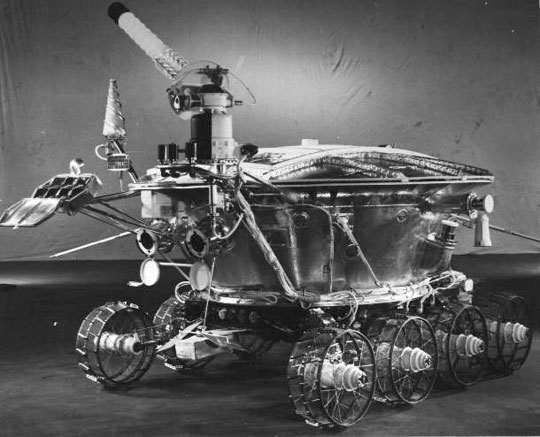
\includegraphics[scale=0.35]{imagenes/Marco Teorico/Lunokhod_1.jpg}
	\caption{Rover sovi�tico Lunokhod 1\cite{Lunokhod1}}
	\label{fig:Lunokhod1}
\end{figure}

Puesto que el principal objetivo de un \textit{rover} es el an�lisis \textit{in situ}, la capacidad de trasladarse, aunque vital, no es suficiente para una misi�n de exploraci�n que obtenga resultados
cient�ficos relevantes. Es por ello que los \textit{rovers} m�s sofisticados como Opportunity y Spirit\cite{RoverMissions}, junto al Curiosity\cite{MissionOverview} y el Perserverance\cite{RoverMars2020} de la NASA, mostradas en la Figura \ref{fig:Rovers}, incorporan un brazo rob�tico que dota al veh�culo con la capacidad de ejecutar diversas tareas, como transportar instrumental de imagen a lugares espec�ficos de inter�s para realizar estudios. Otra aproximaci�n es la de montar un taladro sobre la estructura del \textit{rover} para extraer las muestras, sin embargo esta opci�n limita la versatilidad de la herramienta, dado que depende del posicionamiento del veh�culo en su totalidad, siendo necesario posicionarlo en la ubicaci�n exacta de la muestra, mientras que con el brazo basta con trasladar el efector para que alcance la posici�n deseada.
En el presente documento se desarrolla el dise�o de un manipulador rob�tico, as� como un efector final para identificar mediante visi�n artificial la posici�n de una roca que el usuario le indique para posteriormente obtener informaci�n de ella.

En la Tabla \ref{Tab:Antecedentes} se muestran brazos rob�ticos y efectores finales, que en conjunto pueden formar un sistema rob�tico similar al desarrollado en este documento.

\begin{figure}
	\centering
	\begin{tabular}{cc}
		\subf{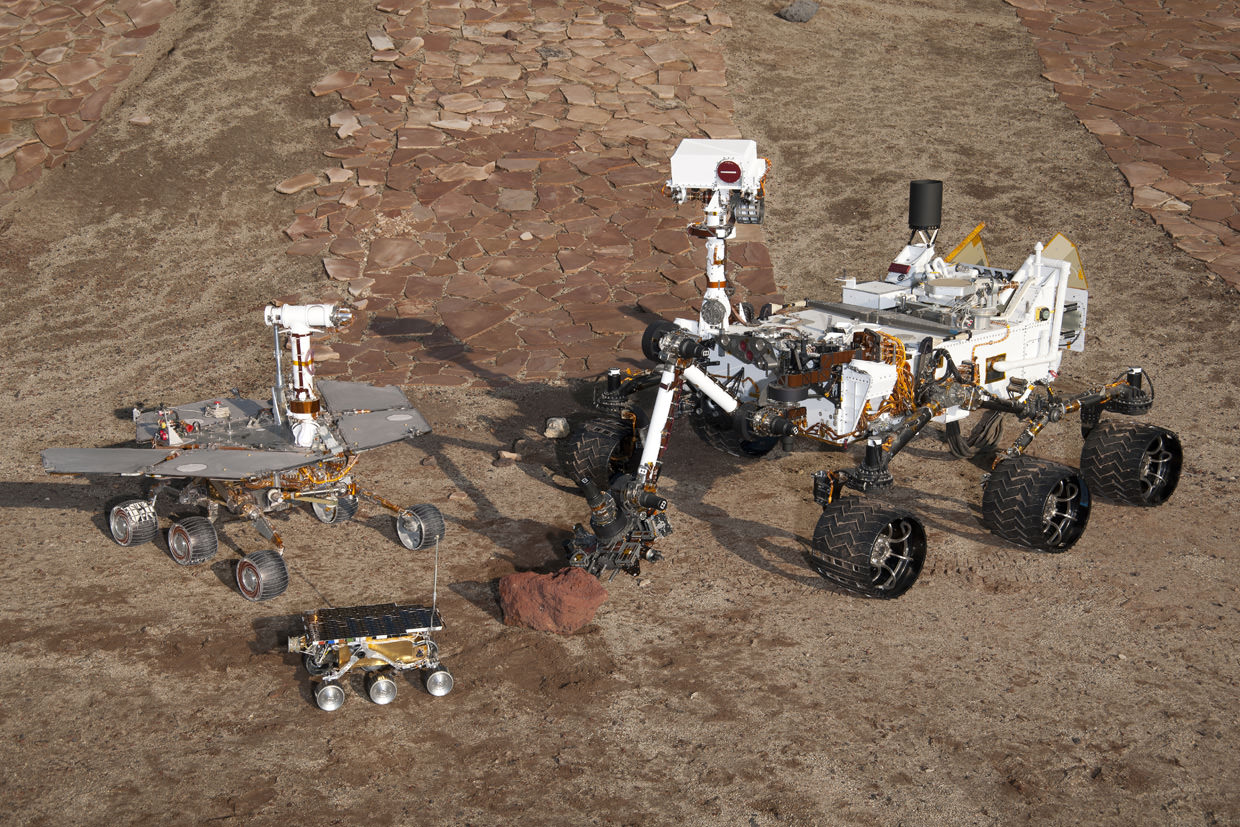
\includegraphics[width=0.45\textwidth, keepaspectratio]{imagenes/Marco Teorico/SpiritOpportunityCuriosity.jpg}}
			{a) Opportunity, Spirit y Curiosity\cite{RoverMissions}}
		&
		\subf{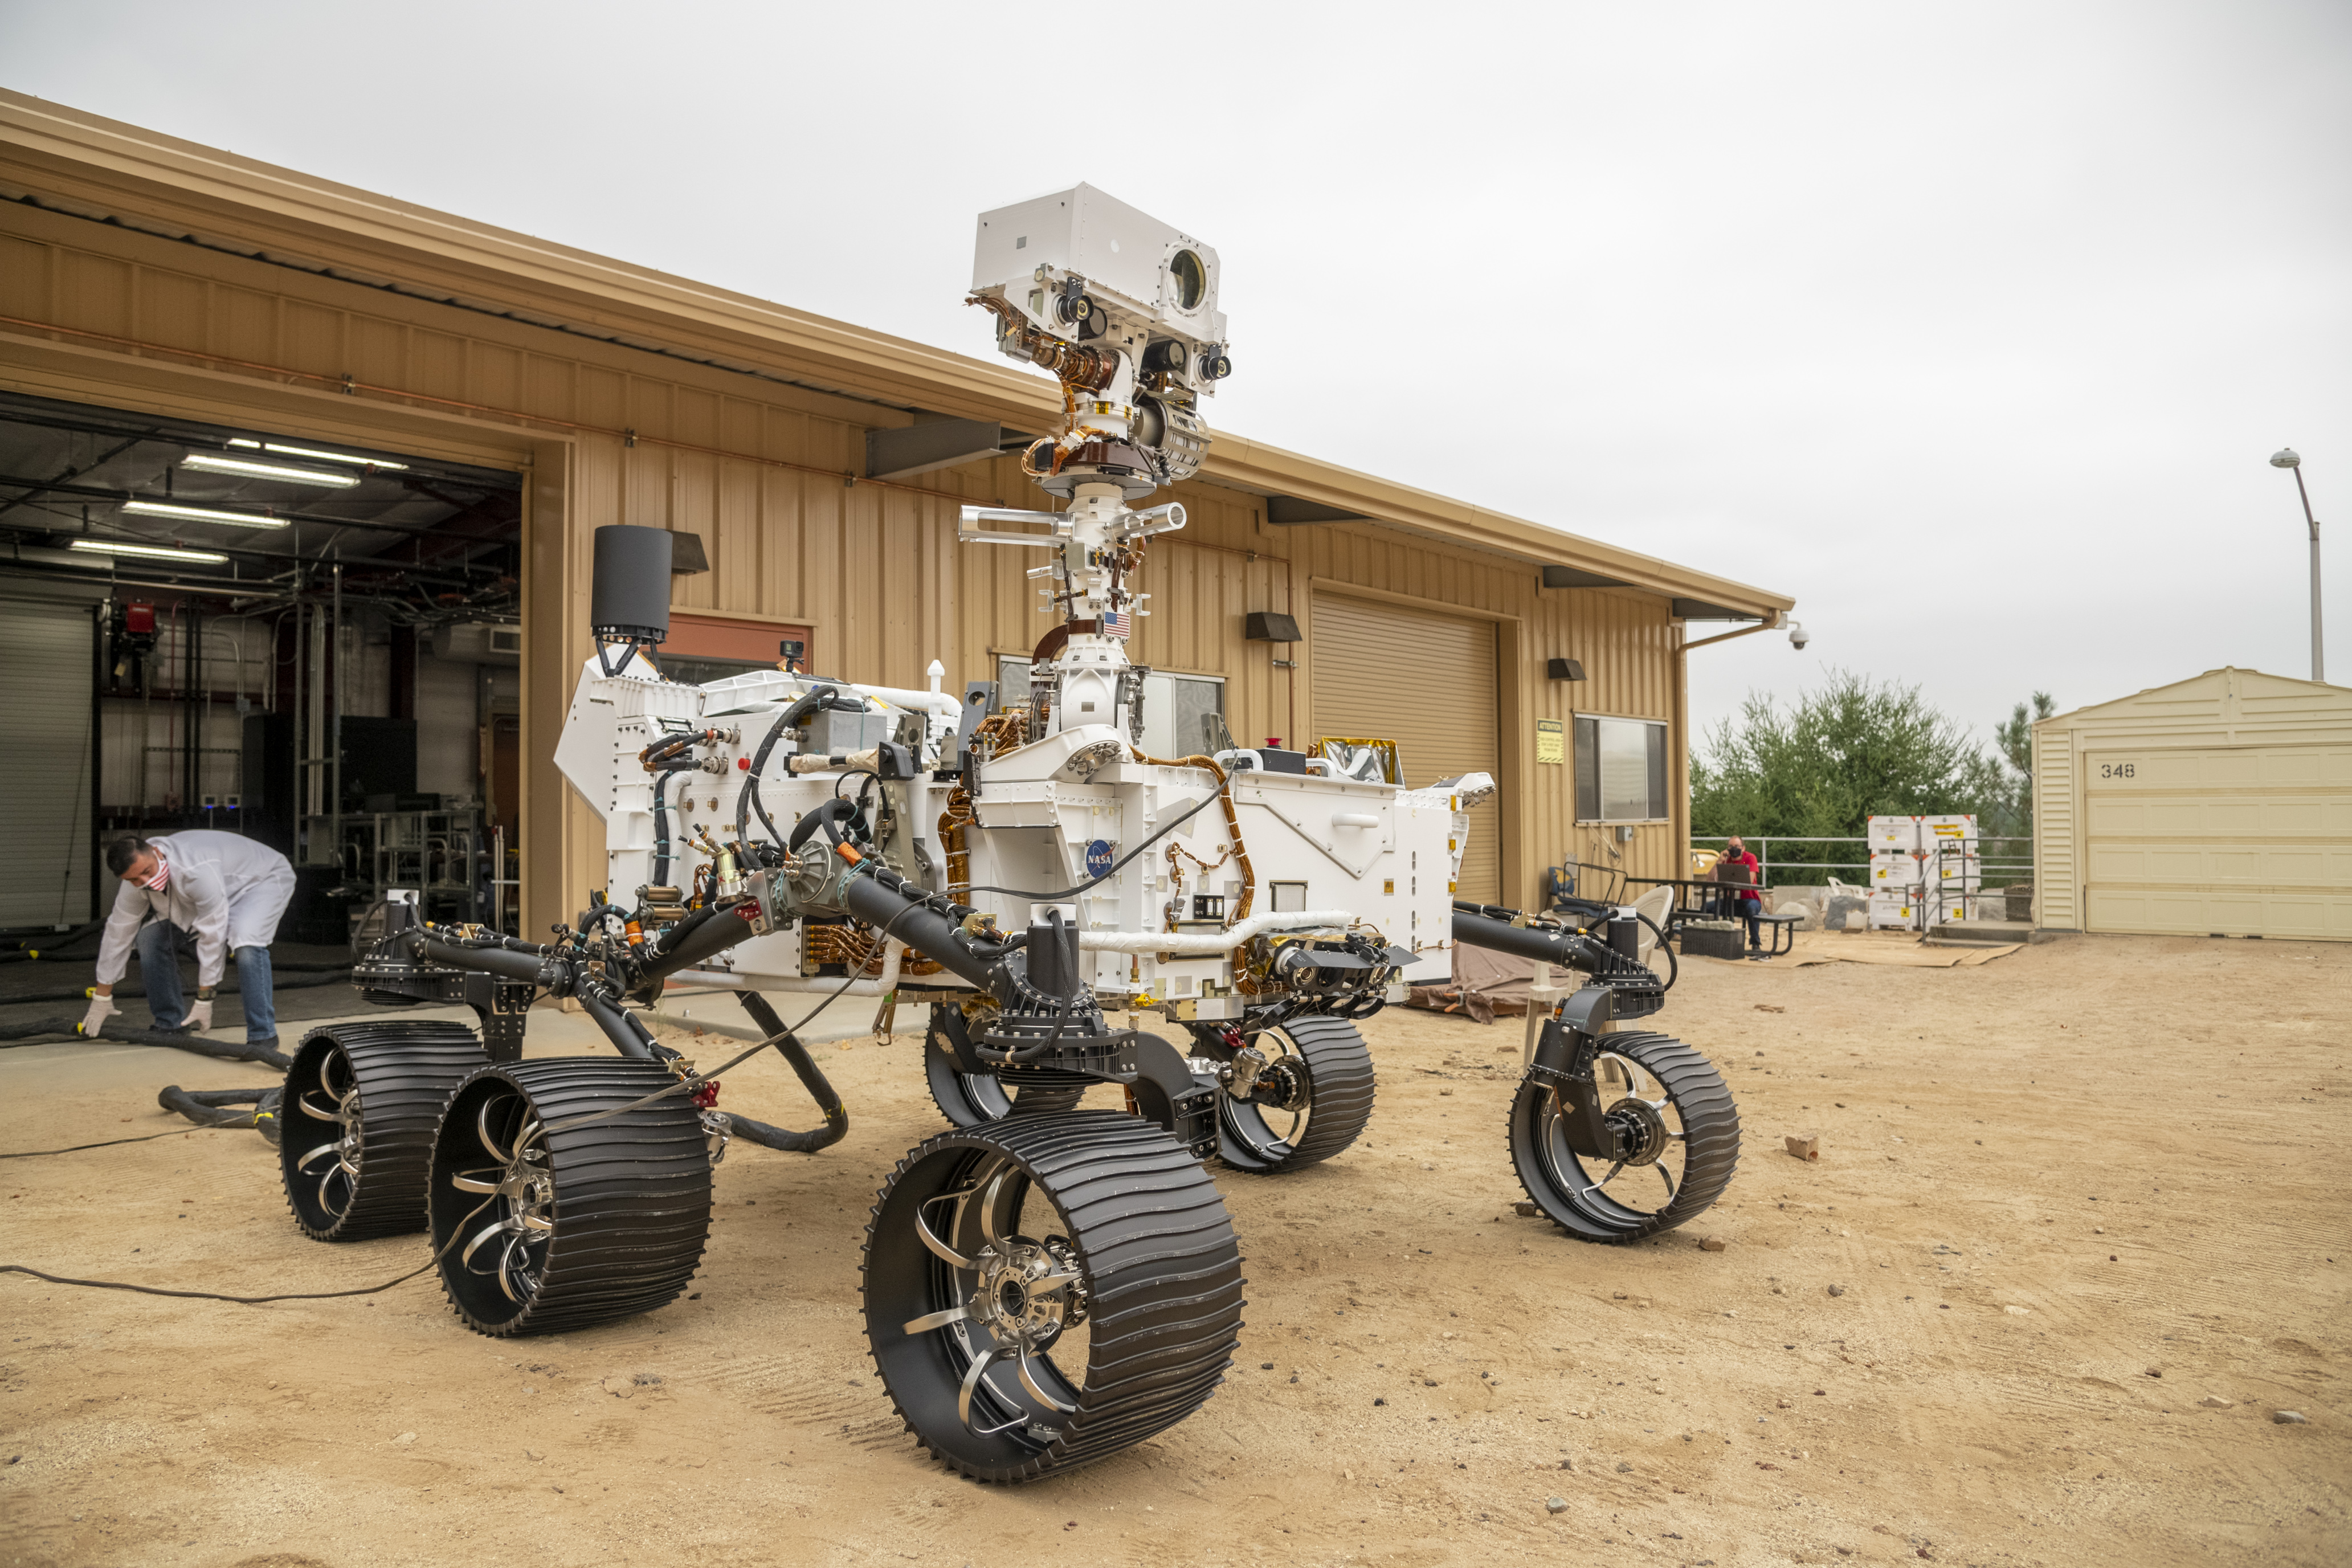
\includegraphics[width=0.45\textwidth, keepaspectratio]{imagenes/Marco Teorico/Perseverance.jpg}}
			{b) Perserverance\cite{RoverMars2020}}
        \\
    \end{tabular}
	\caption{Rovers de la NASA}
	\label{fig:Rovers}
\end{figure}

\section*{Justificaci�n}

La obtenci�n de datos sobre otros cuerpos del sistema solar resulta de vital importancia para
comprender los procesos de formaci�n planetaria y de la evoluci�n de las condiciones
ambientales que han estado presentes a lo largo de su historia. Dichos datos han sido
obtenidos mediante misiones de varios tipos, como los orbitadores que realizan tareas de
cartograf�a, o a trav�s del uso de robots que se colocan en la superficie y son capaces de
obtener muestras \textit{in situ}.
Con el objetivo de probar y validar los dispositivos, las agencias espaciales realizan misiones
an�logas, las cuales son simulaciones del comportamiento del sistema en condiciones
similares a las de operaci�n.
Dado que la obtenci�n de muestras del suelo es una tarea que puede ser realizada mediante
el desarrollo de un sistema rob�tico que posicione un efector adecuado con un error lo
suficientemente peque�o para que tome la muestra deseada, el sistema que efect�e la tarea
debe integrar sistemas el�ctricos, electr�nicos, mec�nicos, de control y de c�mputo. Por lo
tanto, el enfoque mecatr�nico es id�neo para atacar el problema ya que ofrece la capacidad
de integrar todos los sistemas para que trabajen de forma arm�nica, facilitando la
comunicaci�n con otros sistemas, como el \textit{rover} y el analizador, cubriendo las debilidades de
una disciplina con las fortalezas de las otras.

\section*{Definici�n del problema}

Una vez que el robot m�vil ha llegado a la zona de inter�s, el usuario localizar� la muestra en
el espacio de trabajo y el brazo rob�tico deber� llegar a la posici�n y orientaci�n deseada con
el menor error posible, para recoger una muestra y colocarla en un contenedor para su futuro
an�lisis.
Los principales retos de ingenier�a que este proyecto presenta son:

\begin{itemize}[noitemsep,nolistsep]

\item La obtenci�n de una muestra de piedra del suelo, debido a que las rocas no tienen
una geometr�a uniforme.
Aunque el operario identifica la zona donde la muestra est� ubicada, es necesario que
el sistema de reconocimiento del entorno traduzca esa posici�n al espacio de trabajo
del robot.
Para tomar la muestra, hay que conocer la posici�n y orientaci�n, tanto inicial como final
de los actuadores, y generar una trayectoria adecuada tomando en consideraci�n que
la prioridad es el consumo eficiente de energ�a.
Con la finalidad de asegurar la integridad, tanto del actuador como de la muestra, se
requiere conocer la presi�n que el efector ejerce sobre la piedra.

\item El traslado de la muestra obtenida a un sitio concreto, ya que el espacio en el que se
puede manipular es limitado, y se necesita llevar la muestra a un entorno controlado
para poder analizarla.

\item Reducir el consumo energ�tico, pues las celdas incorporadas en los \textit{rover} generan
poco m�s de 100W\cite{RoverPower} para desplazarse y alimentar el resto de m�dulos, por lo que el
sistema debe utilizar una parte de la energ�a disponible.

\item Determinaci�n de la masa de las muestras obtenidas, pues es la informaci�n m�s
esencial que se puede obtener de ellas, por lo cual es necesaria una medida
confiable.

\end{itemize}



\section*{Objetivos}

\subsection*{Objetivo general}
Dise�ar y construir un sistema rob�tico de recolecci�n de muestras geol�gicas para un \textit{rover}
de exploraci�n, que sea capaz de obtener piedras del suelo para su posterior an�lisis y env�o
de datos a una estaci�n.


\subsection*{Objetivos Particulares.}


\begin{enumerate}[noitemsep,nolistsep]
\item Trabajo Terminal I
	\begin{itemize}[noitemsep,nolistsep]
	
	\item Dise�ar un m�dulo a manera de efector final 		que sea capaz de recoger muestras del
	suelo para su manipulaci�n.
	
	\item Dise�ar un sistema rob�tico de 6 grados de 		libertad que posicione y oriente el efector
	para transportar la muestra.

	\item Dise�ar un m�dulo de percepci�n que le 			permita al sistema reconocer el ambiente
	para crear un marco de referencia en el espacio.

	\item Dise�ar un sistema de procesamiento y 			comunicaci�n que permita el an�lisis de las
	muestras para determinar las caracter�sticas del 		entorno, adem�s de permitir la
	transmisi�n y recepci�n de datos. 

	\item Integrar los m�dulos de manera computacional 	para que trabajen en conjunto.

	\item Validar el sistema mecatr�nico mediante 			simulaciones con el objetivo de comprobar
	que los par�metros obtenidos cumplen su funci�n.
	
	\end{itemize}

\item Trabajo Terminal II
	\begin{itemize}[noitemsep,nolistsep]
	
	\item Implementar el m�dulo de efector final que 		sea capaz de recoger muestras del suelo
	para su manipulaci�n.
	
	\item Implementar un sistema rob�tico de 6 grados 		de libertad que posicione y oriente el
	efector para transportar la muestra.

	\item Implementar un m�dulo de percepci�n que le 		permita al sistema reconocer el
	ambiente para crear un marco de referencia en el 		espacio, as� como identificar la
	geometr�a de la muestra.

	\item Implementar un sistema de procesamiento y 		comunicaci�n que permita el an�lisis de
	las muestras para determinar las caracter�sticas 		del entorno, adem�s de permitir la
	transmisi�n y recepci�n de datos.

	\item Realizar pruebas y ajustes necesarios para 		garantizar que cada m�dulo trabaja
	correctamente de manera independiente.

	\item Integrar secuencialmente los m�dulos para 		consolidar el sistema mecatr�nico.

	\item Verificar que todos los m�dulos del sistema 		mecatr�nico trabajen arm�nicamente para
	posteriormente realizar pruebas de recolecci�n de 		muestras en un ambiente an�logo
	que nos permitan comprobar que el sistema cumple 		con la funci�n principal.
	
	\end{itemize}
\end{enumerate} 






\begin{landscape}
\begin{table}
\centering
\tiny
\caption{Antecedentes}
\begin{tabular}{|c|c|c|l|c|c|c|}
\cline{2-7}
\multicolumn{1}{c|}{} & \textbf{Nombre} & \multicolumn{1}{c|}{\textbf{Descripci�n}} & \multicolumn{1}{c|}{\textbf{Caracter�sticas}} & \textbf{Pa�s} & \textbf{Instituto} & \textbf{Tipo} \\
\hline
\textbf{1} & \begin{tabular}[c]{@{}c@{}}Apilador rob�tico\\ aut�nomo de piedras,\\ con planeaci�n de \\posici�n del objeto en \\l�nea.\cite{ANT1}\end{tabular} & \begin{tabular}[c]{@{}l@{}}Sistema rob�tico de brazo con \\efector final capaz de reconocer\\ rocas en el ambiente, orientar el \\efector a fin de asirla, y colocar\\ una encima de otra con un\\ m�ximo de estabilidad.\end{tabular} & \begin{tabular}[c]{@{}l@{}}\begin{tabular}{@{\labelitemi\hspace{\dimexpr\labelsep+0.5\tabcolsep}}l}Manipulador y efector comerciales.~\\Sistema de escaneo �ptico 3D para caracterizar\end{tabular}\\~geom�tricamente las rocas \\(Proceso fuera de l�nea).~\\\begin{tabular}{@{\labelitemi\hspace{\dimexpr\labelsep+0.5\tabcolsep}}l}Algoritmo de b�squeda de la posici�n adecuada\end{tabular}\\~para el apilamiento de la\\piedra (Proceso en l�nea)\\~\end{tabular} & Suiza & ETH Zurich & \begin{tabular}[c]{@{}c@{}}Art�culo de\\ conferencia\end{tabular} \\
\hline
\textbf{2} & Brazo rob�tico UR5\cite{ANT2} & \begin{tabular}[c]{@{}l@{}}M�dulo de brazo rob�tico que se \\adapta al robot Husky para\\ generar una plataforma de \\manipulaci�n m�vil.~\end{tabular} & \begin{tabular}[c]{@{}l@{}}\begin{tabular}{@{\labelitemi\hspace{\dimexpr\labelsep+0.5\tabcolsep}}l}Norma = ISO 10218-1, ISO 13849-1, Cat. 3, PL d.\\Clasificaci�n IP = IP54\\Grados de libertad = 6\\Rango de trabajo de cada eje = 360�\\Carga m�xima = 3 Kg\\Alcance = 500 mm\\Consumo energ�tico = 100 W (T�picamente)\\Rango de temperatura de trabajo = 0�C - 50�C\\Peso total = 11.2 Kg\\Materiales = Aluminio, acero, pl�stico\end{tabular}\end{tabular} & Canad�~ & \begin{tabular}[c]{@{}c@{}}Clearpath\\ Robotics\end{tabular} & Producto \\
\hline
\textbf{3} & \begin{tabular}[c]{@{}c@{}}3-Finger Adaptive\\ Robot Gripper\cite{ANT3}\end{tabular} & \begin{tabular}[c]{@{}l@{}}Gripper de 3 dedos adaptativos\\ para manufactura avanzada e\\ investigaci�n rob�tica~\end{tabular} & \begin{tabular}[c]{@{}l@{}}\begin{tabular}{@{\labelitemi\hspace{\dimexpr\labelsep+0.5\tabcolsep}}l}Apertura de gripper: 0 - 155 mm\\Peso: 2.3 kg\\Carga m�xima recomendada: 10 kg\\Fuerza de agarre: 30 - 70 N\\Modos de agarre\\Puntual\\Ancho\\Tijeras\\B�sico\end{tabular}\end{tabular} & Canad� & Robotiq & Producto~ \\
\hline
\textbf{4} & \begin{tabular}[c]{@{}c@{}}Design of a smart \\gripper for industrial \\applications\cite{ANT4}\end{tabular} & \begin{tabular}[c]{@{}l@{}}Dise�o de un gripper inteligente\\ y flexible para actividades\\ industriales. Adem�s la\\ adaptaci�n de un m�dulo para el \\uso de herramental el�ctrico.\end{tabular} & \begin{tabular}[c]{@{}l@{}}Mediciones en el gripper:\\\begin{tabular}{@{\labelitemi\hspace{\dimexpr\labelsep+0.5\tabcolsep}}l}Fuerza (Galga extensiom�trica)\\Torsi�n en la mu�eca (Sensor de fuerza y~\end{tabular}\\torsi�n de 6 ejes)\\\begin{tabular}{@{\labelitemi\hspace{\dimexpr\labelsep+0.5\tabcolsep}}l}Temperatura~\\Dentro del gripper (LM35)\\Pinzas de sujeci�n (DS18B20)\\Visi�n desde el gripper:\\C�mara (Dragonfly 2 con cabeza extendida)\end{tabular}\\Peso de objetos a manipular:~ 15 kg\\Tipo de agarre del gripper:~\\\begin{tabular}{@{\labelitemi\hspace{\dimexpr\labelsep+0.5\tabcolsep}}l}Dentro del gripper (LM35)\\Pinzas de sujeci�n (DS18B20)\end{tabular}\end{tabular} & Finlandia & \begin{tabular}[c]{@{}c@{}}Tampere \\University of\\ Technology\end{tabular} & \begin{tabular}[c]{@{}c@{}}Tesis de \\maestr�a\end{tabular} \\
\hline
\textbf{5} & \begin{tabular}[c]{@{}c@{}}Mediciones in situ de \\color de suelo, \\composici�n mineral y \\contenido de arcilla por \\espectroscopia VIS-NIR\\ (espectroscopia visible e \\infrarrojo cercano).\cite{ANT5}\end{tabular} & \begin{tabular}[c]{@{}l@{}}An�lisis de propiedades del suelo\\ in situ mediante el uso de\\ espectroscopia infrarroja.\end{tabular} & \begin{tabular}[c]{@{}l@{}}\begin{tabular}{@{\labelitemi\hspace{\dimexpr\labelsep+0.5\tabcolsep}}l}Rango de vis-NIR = 400 - 2500 nm\\Tama�o de grano de la muestra de polvo = 2mm\end{tabular}\end{tabular} & \begin{tabular}[c]{@{}c@{}}Australia \\Francia\end{tabular} & \begin{tabular}[c]{@{}c@{}}-Bruce E. Butler \\Laboratory\\-University of\\ Sydney\\-UMR SAS \\INRA-Agrocam-\\pus Renneser\\ Laboratory\end{tabular} & \begin{tabular}[c]{@{}c@{}}Art�culo de\\ revista\end{tabular} \\
\hline
\end{tabular}
\label{Tab:Antecedentes}
\end{table}


\end{landscape}


\section*{Descripci�n de los cap�tulos}

En el cap�tulo 1, denominado ``Marco de referencia'' se da una breve descripci�n de los fundamentos requeridos para el desarrollo del proyecto, como lo son algunos conceptos de dise�o mec�nico, modelado de robots, visi�n por computador, electr�nica y la metodolog�a de dise�o mecatr�nico.

El cap�tulo 2, ``Dise�o'', toma en cuenta lo siguiente:

2.1: ``Dise�o del sistema'', introduce las necesidades que el sistema debe satisfacer y a partir de ellas desarrollan los requerimiento t�cnicos que sirven como base para generar la arquitectura funcional a trav�s de modelos tales como FBS\cite{FBS}, IDEF0\cite{IDEF0} y eFFBD\cite{eFFBD}. Posteriormente se plantean los m�dulos que conforman al sistema mecatr�nico, y a partir de ellos se proponen soluciones que se someten a una herramienta de selecci�n multi-criterio para encontrar la que mejor satisface los criterios establecidos.

2.2: ``Dise�o de dominio espec�fico'', se realiza un dise�o a profundidad de cada uno de los m�dulos que conforman el concepto soluci�n elegido en el cap�tulo 2.

2.3: ``Integraci�n del sistema mecatr�nico'', se realiza la uni�n de los m�dulos dise�ados para asegurar que cada una de las partes del sistema opera de manera arm�nica con las dem�s. Este proceso se realiza siguiendo una secuencia que inicia con el hardware y concluye con el software.

En el cap�tulo 3, ``Implementaci�n'' se describe detalladamente el proceso de fabricaci�n del sistema, as� como la realizaci�n de una fase de pruebas para detectar y solucionar problemas a trav�s de redise�os con el fin de garantizar el cumplimiento de la funci�n principal.

Finalmente, en el cap�tulo 4 se analizan los resultados de las simulaciones computacionales para determinar si se cumplen los objetivos.

          %%%modificar archivo introduccion.tex
%%%%%Antecedentes
%%%%%Planteamiento del problema
%%%%%Descripci�n de los cap�tulos
%%%%%%%%%%%%%%%%%%%%%%%%%%%%%%%%%%%%%%%%%
%%%%%% Inicia Contenido del trabajo%%%
%\formatodoc%
\mainmatter

%\pagestyle{fancy}
%\renewcommand{\chaptermark}[1]{\markboth{#1}{}}
%\renewcommand{\sectionmark}[1]{\markright{#1}}
%\fancyhf{}
%\fancyhead[RO]{\rightmark}
%\fancyhead[LE]{\leftmark}
%\fancyhead[LO,RE]{}
%\fancyfoot{}
%\fancyfoot[RO,LE]{\thepage}
%\fancyfoot[CO]{UPIITA}
%\fancyfoot[CE]{IPN}
%\fancyfoot[RE,LO]{Ing. Mecatr�nica}
%%%%%%%%%%%%%%%%%%%%%%%%%%%%%%%%%%%%%%%%%%%%%%%%%%%%%%%%%%%%%%%%%%%
%%%%%%%%%%%%%%%%%%%%%%%%%%capitulo1111111111%%%%%%%%%%%%%%%%%%%%%%%

%\layout
%\pagevalues
%\pagedesign
\chapter{Marco de referencia}

\section{Marco te�rico}

\subsection{Descripci�n de forma de part�culas}

Medir dimensiones y caracter�sticas de part�culas individuales es un proceso tardado y costoso, por ellos existen escalas cualitativas que permiten una r�pida evaluaci�n visual de la misma. Dichas tablas eval�an par�metros como la angularidad y esfericidad. De acuerdo a \cite{Esfericidad}, una escala como esta es usada en la norma ASTM F1632 2003, como se muestra en la Figura \ref{fig:Esfericidaddd}.

\begin{figure}
\centering		
	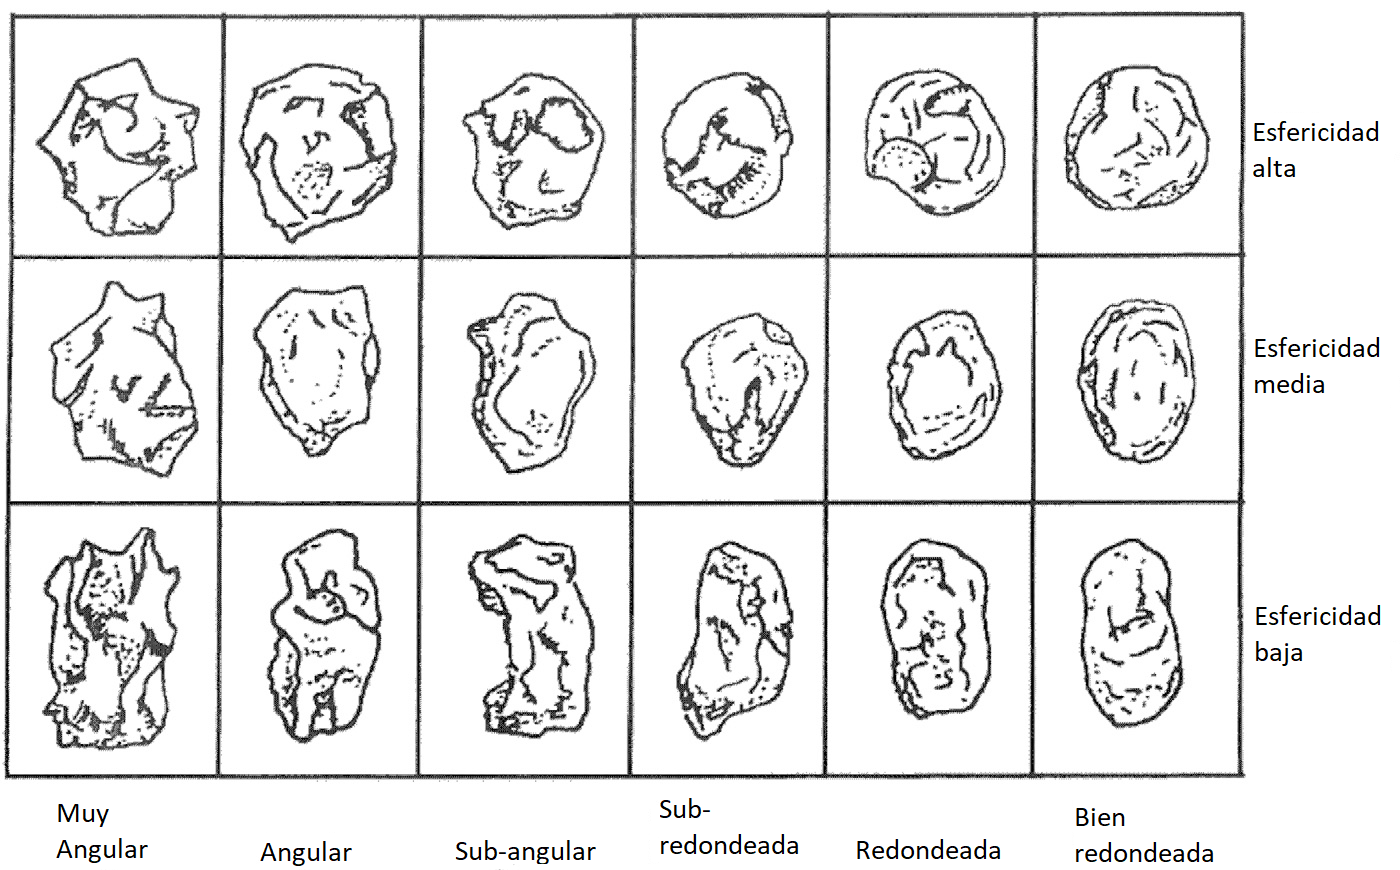
\includegraphics[scale=0.3]{imagenes/Marco Teorico/Esfericidad}
	\caption{Cuadro cualitativo para determinar visualmente la forma de una part�cula}
	\label{fig:Esfericidaddd}
\end{figure}

\subsection{Dise�o de componentes de m�quinas}

\subsubsection{Selecci�n de materiales}

Las propiedades mec�nicas de los materiales influyen en el desempe�o de los componentes f�sicos, por esta raz�n es necesario tomar en cuenta sus l�mites para el dise�o. Adem�s es importante considerar la relaci�n existente entre las propiedades, pues suele tomarse en cuenta la combinaci�n de ellas para realizar la selecci�n.

En este documento, son de particular inter�s las propiedades de rigidez y densidad, por lo que se utiliza la relaci�n entre el m�dulo de Young y la densidad\cite{Ashby}, mostrada gr�ficamente en la Figura \ref{fig:DensidadVSYoung}.

\begin{figure}
\centering		
	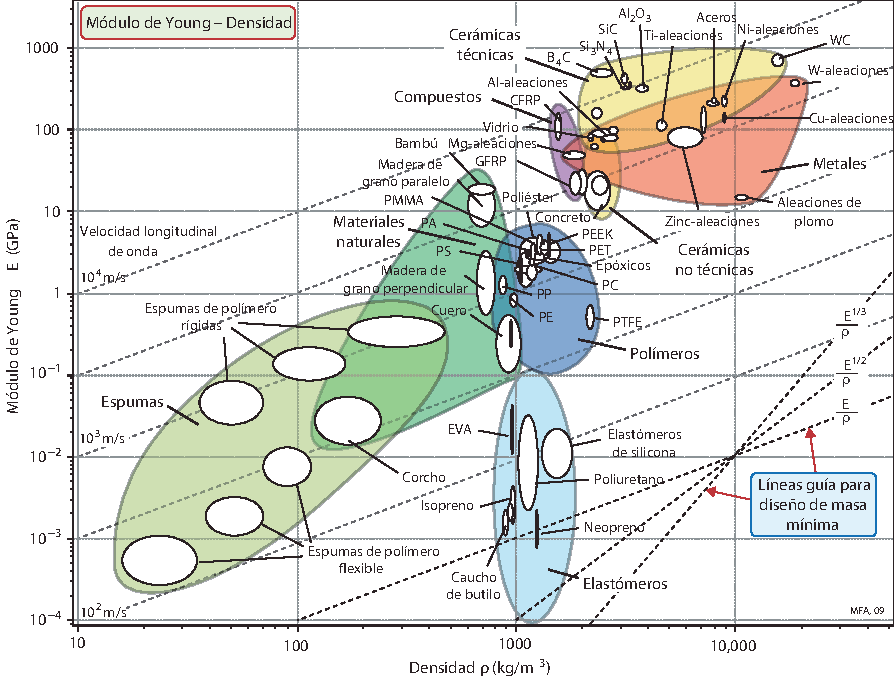
\includegraphics[scale=1]{imagenes/Dominio especifico/DensidadVSYoung_Ashby}
	\caption{Gr�fico que relaciona el m�dulo de elasticidad de los materiales contra su densidad, Ashby.}
	\label{fig:DensidadVSYoung}
\end{figure}

\subsubsection{Dise�o de transmisi�n por bandas}

Para seleccionar las bandas a usar, se debe establecer la relaci�n de velocidades entre la polea conductora y la polea conducida, adem�s del par que el motor suministra.

La velocidad tangencial de un objeto que gira se relaciona con la velocidad angular seg�n la ecuaci�n: 

\begin{align}
\label{eq:VTang}
& v = \omega \times r
\end{align}

Posteriormente, se calcula la potencia necesaria que la banda debe transmitir (ecuaci�n \ref{eq:PotBanda}), as� como el factor de servicio que se obtiene de tablas\cite{Mott}, con base en la aplicaci�n, el tipo de motor y el tiempo de operaci�n, calculando la potencia de dise�o con la ecuaci�n \ref{eq:PotDis}.

\begin{align}
\label{eq:PotBanda}
P &= \tau \omega =
\end{align}

\begin{align}
\label{eq:PotDis}
P_{ajustada} &= P*F_S 
\end{align}

Posteriormente, se determina el paso requerido de la banda utilizando la gu�a de selecci�n de perfil del proveedor\cite{BandasSDPSI}, mostrada en la Figura \ref{fig:PasoBanda}.

\begin{figure}
\centering		
	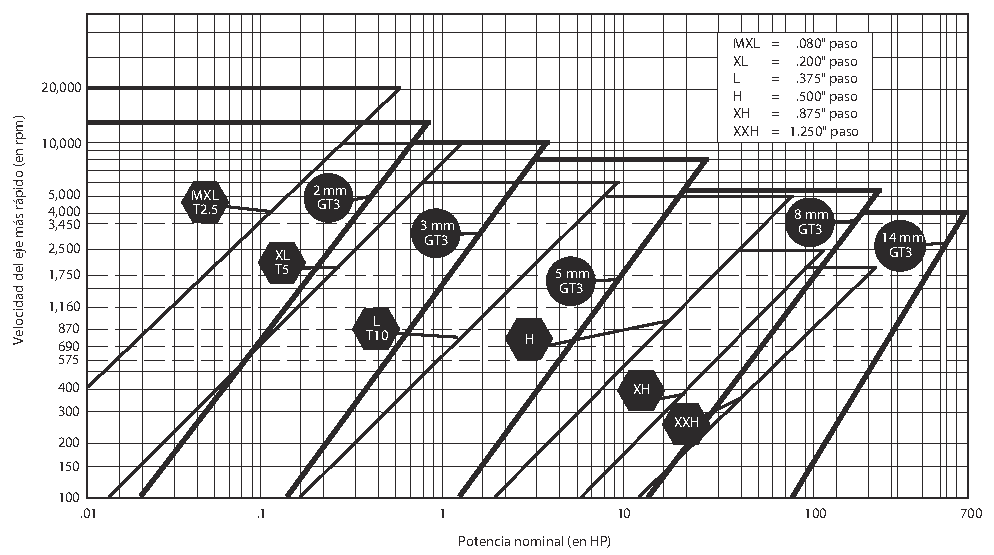
\includegraphics[scale=0.85]{imagenes/Dominio especifico/Validaciones eslabones/Transmision/PerfilesBandas}
	\caption{Gu�a de selecci�n de paso de bandas}
	\label{fig:PasoBanda}
\end{figure}

Seleccionar la combinaci�n de poleas que producen la relaci�n de velocidad especificada, bas�ndose en el cat�logo de proveedores \cite{PoleasSDPSI}, en el cual tambi�n se indica el ancho apropiado de las bandas.

Conociendo el di�metro de las poleas seleccionadas, se calcula la longitud de la banda como sigue:

\begin{align}
\label{eq:LongBanda}
L_{b} &=  2C+N_{polea}*PD
\end{align}

\begin{align*}
\textrm{En donde:}\\
L_{b} &= \textrm{Longitud de la banda.}\\
C &= \textrm{Distancia entre centros.}\\
N_{polea} &= \textrm{N�mero de dientes de la polea.}\\
PD &= \textrm{Paso.}
\end{align*}

Con la longitud de la banda calculada, se ajusta el valor de la potencia con la ecuaci�n \ref{eq:PotBandAjus}.

\begin{align}
\label{eq:PotBandAjus}
& \textrm{Potencia base nominal}_{ajustada} =
\end{align}

\begin{align*}
& \textrm{Potencia base nominal} * \textrm{Factor de correcci�n de longitud}
\end{align*}

Finalmente, se calcula la velocidad lineal de las bandas para comprobar que operan con niveles bajos de ruido, como sigue:

\begin{align}
\label{eq:VelBandRuido}
V_{banda-1}&=\frac{PD_{1}}{2}*\omega_{1}\\
V_{banda-2}&=\frac{PD_{2}}{2}*\omega_{2}
\end{align} 

\subsubsection{Dise�o de ejes}

El dise�o de un eje consiste en determinar el di�metro m�nimo para un estado de esfuerzos est�tico. Primero se obtienen los esfuerzos debidos a momentos flectores, para buscar el momento flector m�ximo para todos los di�metros diferentes del eje\cite{Mott}. Despu�s se consideran los momentos torsionantes a los que est� sometido el eje.

Para calcular el momento flector, deben tomarse en cuenta las tensiones que las bandas ejercen sobre el eje a trav�s de las poleas, utilizando las ecuaciones

\begin{align}
\label{eq:FuerzaBanda}
F_{n} &= \frac{T_{banda}}{r}\\
F_{s} &= 1.5F_{n}
\end{align}

\begin{align*}
\textrm{En donde:}\\
F_{n} &= \textrm{Fuerza neta asociada al torque transmitido}\\
F_{s} &= \textrm{Fuerza flexionante}\\
T_{banda} &= \textrm{Torque transmitido por la banda}\\
r &= \textrm{Radio de la polea}
\end{align*}

Una vez que se obtienen estos valores, se propone un material y se corrigen los valores de resistencia �ltima a fatiga con las ecuaciones \ref{eq:Sn} y \ref{eq:SnC}.

\begin{align}
\label{eq:Sn}
S_{n} &=0.5S_{u}
\end{align}

\begin{align*}
\textrm{En donde:} \\
S_{n} &= \textrm{L�mite de fatiga}\\
S_{u} &= \textrm{Esfuerzo �ltimo a la tensi�n}
\end{align*}

\begin{align}
\label{eq:SnC}
S'_{n} &= S_{n}C_{m}C_{st}C_{R}C_{s} 
\end{align}

\begin{align*}
\textrm{En donde:} \\
S'_{n} &= \textrm{L�mite de fatiga modificado}\\
C_{m} &= \textrm{Factor de material}\\
C_{st} &= \textrm{Factor de tipo de esfuerzo}\\
C_{R} &= \textrm{Factor de confiabilidad}\\
C_{s} &= \textrm{Factor de tama�o}
\end{align*}

Finalmente, se utiliza la f�rmula \ref{eq:DiamEje} para calcular el di�metro m�nimo del eje.

\begin{align}
\label{eq:DiamEje}
D &=\sqrt[3]{\frac{32N}{\pi}\sqrt{\left[ \frac{K_{t}M}{S'_{n}}^{2} \right] + \frac{3}{4} \left[ \frac{T}{S_{y}} \right]^{2} }}
\end{align}

\begin{align*}
\textrm{En donde:} \\
D &= \textrm{Di�metro m�nimo del eje}\\
N &= \textrm{Factor de seguridad}\\
K_{t} &= \textrm{Factor de concentraci�n de esfuerzos}\\
M &= \textrm{Momento flexionante}\\
T &= \textrm{Esfuerzo torsionante}\\
S_{y} &= \textrm{Esfuerzo de cedencia}
\end{align*}

\subsubsection{Selecci�n de rodamientos}

Para seleccionar rodamientos aleados, es necesario conocer las reacciones que tienen ante las fuerzas del eje, utilizando la ecuaci�n \ref{eq:RodamientosAleados} para conocer la carga din�mica, que es el dato que ofrece el fabricante para su selecci�n.

\begin{align}
\label{eq:RodamientosAleados}
C_{din\acute{a}mica} &= P_{d} \left( \frac{L_{d}}{10^{6}}\right)^{1/k_{rod}}
\end{align}

\begin{align*}
\textrm{En donde:} \\
C_{din\acute{a}mica} &= \textrm{Capacidad de carga din�mica m�nima del rodamiento}\\
P_{d} &= \textrm{Carga de dise�o}\\
L_{d} &= \textrm{Vida de dise�o del rodamiento, en n�mero de revoluciones}\\
k_{rod} &= 3.33 \textrm{ para rodamientos de rodillos}
\end{align*}

\subsection{Cinem�tica de robots}

Para conocer la manera en la que el manipulador se mueve, es necesario identificar las relaciones que hay entre los diferentes grados de libertad que lo conforman, en este apartado se desarrolla dicha relaci�n desde un enfoque puramente geom�trico, conocido como cinem�tica del robot, sin tomar en cuenta las fuerzas y torques que generan los movimientos, pues estos se tomar�n en cuenta para desarrollar la din�mica del robot.

\subsubsection{Cinem�tica directa}

Como ya se mencion�, el modelo cinem�tico sirve para describir geom�tricamente el movimiento del manipulador, para lo que se considera en primer lugar el problema de la cinem�tica directa, la cual describe la posici�n y orientaci�n del efector final dados los valores de las variables de las juntas del robot. 

Una matriz de transformaci�n homog�nea representa una traslaci�n y rotaci�n de un marco coordenado $n$ con respecto de un marco base $0$, y est� definida por la ecuaci�n \ref{eq:MTH}.

\begin{align}
\label{eq:MTH}
H&=
\begin{bmatrix}
R_{n}^{0} & o_{n}^{0} \\
0 & 1
\end{bmatrix}
\end{align}

Para calcular esta matriz, se utilizan matrices de la forma

\begin{align*}
A_{i}&=
\begin{bmatrix}
R_{i}^{i-1} & o_{i}^{i-1} \\
0 & 1
\end{bmatrix}
\end{align*}

las cuales relacionan al marco $i$ con respecto al marco $i-1$, el cual se obtiene al acoplar r�gidamente un marco de referencia a cada junta del sistema.

De esta manera, la matriz de la ecuaci�n \ref{eq:MTH} se puede descomponer en una serie de transformaciones, como se ve en la ecuaci�n \ref{eq:HTA}.

\begin{align}
\label{eq:HTA}
H &= T_{n}^{0} = A_{1}( \theta_{1} ) \dots A_{n}\theta_{n}
\end{align}

Para facilitar la asignaci�n de marcos y la obtenci�n de las matrices se utiliza la convenci�n de Denavit-Hartenberg, asumiendo lo siguiente:

\begin{itemize}[noitemsep,nolistsep]
\item El eje $x_{1}$ es perpendicular al eje $z_{0}$
\item El eje $x_{1}$ se interseca con el eje $z_{0}$
\end{itemize}

De esta manera, se puede representar la transformaci�n $H$ de la ecuaci�n \ref{eq:MTH} con matrices de la forma:

\begin{align*}
A_{i} &= 
\begin{bmatrix}
c_{\theta_{i}} & -s_{\theta_{i}}c_{\alpha_{i}} & s_{\theta_{i}}s_{i} & a_{i}c_{\theta_{i}}\\
s_{\theta_{i}} & c_{\theta_{i}}c_{\alpha_{i}} & -c_{\theta_{i}}s_{\alpha_{i}} & a_{i}s_{\theta_{i}}\\
0 & s_{\alpha_{i}} & c_{\alpha_{i}} & d_{i}\\
0 & 0 & 0 & 1\\
\end{bmatrix}
\end{align*}

\begin{align*}
\textrm{En donde:}\\
\theta &= \textrm{�ngulo de la junta, formado entre} \; x_{i-1} \; \textrm{y} x_{i} \; \textrm{sobre el eje} \; z_{i-1}. \\
a &= \textrm{Longitud del eslab�n, definido como la distancia sobre el eje} \; x_{i} \\
& \quad\; \textrm{desde el punto de intersecci�n de} \; z_{i-1} \; \textrm{con} \; x_{i} \; \textrm{hasta el origen} \; O_{i}. \\
d &= \textrm{Desplazamiento del eslab�n, definido como la distancia sobre el eje} \; z_{i-1} \\
& \quad\; \textrm{desde el origen} \; O_{i-1} \; \textrm{hasta la intersecci�n de} \; z_{i-1} \; \textrm{con} \; x_{i}. \\
\alpha &= \textrm{�ngulo de giro del eslab�n, formado entre} \; z_{i-1} \; \textrm{y} \; z_{i} \; \textrm{sobre el eje} \; x_{i}.
\end{align*}

\subsubsection{Cinem�tica inversa}

Una vez que se ha resuelto el problema de cinem�tica directa, se puede realizar el proceso contrario, conocido como cinem�tica inversa, utilizado para conocer los valores de las variables de las juntas dada la posici�n y orientaci�n del efector final.

Esto significa que de la ecuaci�n \ref{eq:MTH}, se conoce el valor de $H$, y el objetivo es encontrar el valor de $R_{n}^{0}(\theta_{1}\dots\theta_{n})$ y $o_{n}^{0}(\theta_{1}\dots\theta_{n})$.

En los sistemas rob�ticos con una mu�eca esf�rica, los ejes de las 3 �ltimas juntas se intersecan en un punto, en el cual se asignan los or�genes de los marcos de referencia 3,4 y 5. Esto se conoce como \textit{desacoplamiento cinem�tico}, y permite separar el problema de cinem�tica inversa en 2 problemas m�s sencillos de resolver, conocidos como \textit{cinem�tica inversa de posici�n} y \textit{cinem�tica inversa de orientaci�n}.

Para realizar este procedimiento, se interpreta que:

\begin{align}
\label{eq:DesCin}
R_{n}^{0}(\theta_{1} \dots \theta_{n}) &= R\\
\label{eq:DesCin2}
o_{n}^{0}(\theta_{1} \dots \theta_{n}) &= o
\end{align}

Siendo

\begin{align}
\label{eq:RTarget}
R=
\left[
\begin{array}{ccc}
r_{11} & r_{12} & r_{13}\\
r_{21} & r_{22} & r_{23}\\
r_{31} & r_{32} & r_{33}
\end{array}
\right]\\
o=
\begin{bmatrix}
ox\\oy\\oz
\end{bmatrix}
\end{align}

\textbf{Cinem�tica inversa de posici�n}

Desplazando una distancia $d_{6}$ el efector final $o$ hacia el origen de la mu�eca $o_{c}$, se puede resolver $R_{3}^{0}$ como sigue:

\begin{align}
o &= o_{c}^{0} + d_{6}R\begin{bmatrix}
0\\0\\1
\end{bmatrix}
\end{align}

\textbf{Cinem�tica inversa de orientaci�n}

Conociendo $R_{3}^{0}$ se puede calcular $\theta_{1}$, $\theta_{2}$ y $\theta_{3}$, permitiendo resolver la ecuaci�n \ref{eq:R06Pieper} para conocer $\theta_{4}$, $\theta_{5}$ y $\theta_{6}$

\begin{align}
\label{eq:R06Pieper}
R_{6}^{3} = \left(R_{3}^{0}\right)^{T}R
\end{align}

\subsubsection{Cinem�tica diferencial - El Jacobiano}

Matem�ticamente la cinem�tica directa define una funci�n entre el espacio de posiciones y orientaciones del efector final y el espacio de posiciones de las juntas. Las relaciones de velocidad est�n determinadas por el jacobiano de esta funci�n. 

La matriz Jacobiana para una junta de tipo revoluta est� dada como sigue:

\begin{align}
J_{i} &= \begin{bmatrix}
 z_{i-1} \times (o_{n}-o_{i-1})\\   z_{i-1} 
\end{bmatrix}
\label{eq:JacRev}
\end{align}

El robot desarrollado en este proyecto tiene solo juntas de tipo revoluta. Todas las variables implicadas en la determinaci�n del Jacobiano est�n disponibles una vez que se ha ejecutado la cinem�tica directa. 

Singularidades.

El rango de la matriz Jacobiana no es constante, pues depende de la configuraci�n de las juntas del robot. Las configuraciones para los cuales el Jacobiano pierde rango se llaman singularidades, y su identificaci�n es importante porque:
\begin{itemize}[noitemsep,nolistsep]
\item[a)]	Pueden representar configuraciones para las cuales ciertas direcciones de movimiento son inalcanzables.
\item[b)]	La velocidad de movimiento de las juntas puede diverger conforme se acercan a una posici�n singular.
\item[c)]	En las singularidades, fuerzas y momentos acotados del efector final pueden requerir fuerzas y momentos divergentes en las juntas.
\item[d)]	Las singularidades usualmente (aunque no siempre) corresponden a puntos en la frontera del espacio de trabajo del manipulador, es decir, los puntos de m�ximo alcance del manipulador.
\item[e)]	Las singularidades corresponden a puntos en el espacio de trabajo del manipulador que pueden ser inalcanzables bajo peque�as perturbaciones en los par�metros de los eslabones, tales como desplazamiento, longitud, etc.
\item[f)]	Cerca de las singularidades, no existir� una �nica soluci�n al problema de cinem�tica inversa. En tales casos puede no haber soluciones o existir infinitas. 
\end{itemize}

El problema de resolver la ecuaci�n no lineal $det J(q)=0$ puede ser complicado, pero es posible utilizar una t�cnica que explota el hecho de tener una mu�eca esf�rica, conocidad como desacoplamiento de singularidades. 
Si el n�mero de grados de libertad es igual a 6, y tres de ellos corresponden al brazo y 3 de ellos a la mu�eca esf�rica, el Jacobiano consistir� en una matriz de 6x6, como es una matriz cuadrada, ser� singular cuando $det(J)=0$.

Si se parte la matriz en segmentos de 3x3, se tiene: 

\begin{align}
J &=\begin{bmatrix}
J_{P}&| & J_{O}
\end{bmatrix} =
\begin{bmatrix} 
	\begin{array}{cc|cc}
	J_{11} &&& J_{12} \\
	\hhline{|-|~|~|-|}
	J_{21} &&& J_{22}
	\end{array}
\end{bmatrix}
\label{eq:JPO}
\end{align}

Como los �ltimos tres GDL son revoluta

\begin{align}
J_{O} &= \begin{bmatrix}
 z_{3} \times (o_{3}-o_{3})& z_{4} \times (o_{3}-o_{3}) & z_{5} \times (o_{3}-o_{3}) \\  z_{3}
 &  z_{4} &  z_{5}
\end{bmatrix}
\label{eq:JO}
\end{align}

Y ya que los ejes se intersectan en el mismo punto, se considera que los or�genes de los marcos de referencia del 3 al 6 est�n en el mismo punto, se vuelve

\begin{align}
J_{O} &= \begin{bmatrix}
 0& 0 & 0 \\  z_{3}
 &  z_{4} &  z_{5}
\end{bmatrix}
\label{eq:JO2}
\end{align}

Este caso, el Jacobiano se convierte en una forma triangular

\begin{align}
J &= \begin{bmatrix}
 J_{11}& 0   \\ 
J_{21} &  J_{22}
\end{bmatrix}
\label{eq:JTriang}
\end{align}

Y cuyo determinante se simplifica

\begin{align}
det (J)=det(J_{11})det(J_{22})
\label{eq:detJ}
\end{align}

De forma que las singularidades del sistema son las singularidades del brazo $det J_{11}=0$ y de las singularidades de la mu�eca $det J_{22}=0$.

Cabe se�alar que esta forma de Jacobiano solo sirve para la determinaci�n de singularidades, pues no se corresponde con la matriz que relaciona la velocidad el efector final con las velocidades de las juntas, ya que usa la suposici�n de que $o_{6}$ est� en el mismo punto que $o_{5}$, lo cual no es cierto, pues est� desplazado por una distancia $d$. 

\subsection{Din�mica de robots}

Mientras que la cinem�tica de robots describe el movimiento de robots sin considerar las fuerzas y torques involucrados, las ecuaciones din�micas relacionan expl�citamente estas fuerzas con el movimiento.

Si el lector desea conocer a detalle la deducci�n anal�tica de los t�rminos tratados tanto en esta secci�n como en la de cinem�tica, en \cite{Spong} se desarrolla ampliamente.

En este documento se aborda el tema de din�mica de robots a trav�s del enfoque de Euler-Lagrange, que calcula la din�mica a trav�s de la diferencia entre la energ�a cin�tica y potencial del sistema con la ecuaci�n \ref{eq:EulerLagrangeGeneral}, aunque se puede encontrar f�cilmente en la literatura el enfoque de Newton-Euler, que realiza este c�lculo a trav�s de las reacciones presentes en los cuerpos\cite{Spong}.

\begin{align}
\label{eq:EulerLagrangeGeneral}
\frac{d}{dt}\left(\frac{\partial \mathcal{L}}
{\partial\dot \theta}\right)
-\frac{\partial \mathcal{L}}{\partial \theta}=\mathcal{Q}
\end{align}

\begin{align*}
\textrm{En donde:}\\
\mathcal{L} &= \textrm{Lagrangiano del sistema}\\
\theta &= \textrm{Conjunto de coordenadas generalizadas}\\
\mathcal{Q} &= \textrm{Conjunto de fuerzas generalizadas}
\end{align*}

Las coordenadas generalizadas $\theta$ son aquellas que describen el movimiento del robot, y tienen las siguientes caracter�sticas \cite{MITDyn}:

\begin{itemize}[noitemsep,nolistsep]
\item No necesitan ser cartesianas
\item No necesitan ser inercialmente sim�tricas, i.e. sus momentos de inercia pueden describirse con matrices no diagonales.
\item Deben ser independientes, i.e. si se fijan todas la coordenadas generalizadas excepto por una, el grado de libertad descrito por esa coordenada a�n tiene un rango continuo de movimiento.
\item Deben ser completas, i.e. siempre son capaces de localizar todas las partes del robot.
\item Deben ser holon�micas, i.e. el n�mero de coordenadas generalizadas es igual al n�mero de grados de libertad del robot.
\end{itemize}

De acuerdo al desarrollo de la cinem�tica directa, es posible comprobar que los par�metros de Denavit-Hartenberg cumplen con estas caracter�sticas y, por lo tanto, sirven como un conjunto de coordenadas generalizadas\cite{Spong}.

Para encontrar las fuerzas generalizadas $\mathcal{Q}_{i}$ ligadas a las coordenadas generalizadas $\theta_{i}$, resulta �til utilizar el \textit{Principio de Trabajo Virtual}, que indica que el trabajo realizado por fuerzas externas (no conservativas) correspondiente a cualquier conjunto de desplazamientos virtuales es igual a cero\cite{Spong}.

\begin{align}
\label{eq:TrabajoVirtual}
\delta W^{NC}_{i} &= \mathcal{Q}_{i} \delta_{\theta_{i}} = 0 
\end{align}

\begin{align*}
\textrm{En donde:}\\
\delta W^{NC}&=\textrm{Trabajo virtual asociado a las fuerzas generalizadas }\mathcal{Q}\\
\delta \theta &= \textrm{Desplazamientos virtuales}
\end{align*}

Para calcular las ecuaciones din�micas que describen el movimiento del robot utilizando el sistema de ecuaciones diferenciales ordinarias de segundo orden presentado en la ecuaci�n \ref{eq:EulerLagrangeGeneral}, es necesario expresar las energ�as cin�tica y potencial en t�rminos de las coordenadas y fuerzas generalizadas $\theta$ y $\mathcal{Q}$ respectivamente. A continuaci�n se desarrollan las f�rmulas necesarias para lograr esto.

\subsubsection{Energ�a cin�tica}
La energ�a cin�tica de un cuerpo r�gido es la suma de la energ�a traslacional obtenida al concentrar la masa del cuerpo en su centro de masa, y la energ�a rotacional alrededor del mismo. Esta suma se presenta en la ecuaci�n \ref{eq:KGeneral}.

\begin{align}
\label{eq:KGeneral}
K &= \frac{1}{2} mv^{T}v+\frac{1}{2}\omega^{T}\mathcal{I}\omega
\end{align}

\begin{align*}
\textrm{En donde:}\\
K &= \textrm{Energ�a cin�tica}\\
m &= \textrm{Masa total}\\
v &= \textrm{Vector de velocidad lineal}\\
\omega &= \textrm{Vector de velocidad angular}\\
\mathcal{I} &= \textrm{Tensor de inercia}
\end{align*}

El tensor de inercia $\mathcal{I}$ es una matriz sim�trica de $3 \times 3$ expresado en el marco inercial del objeto, por lo depende de la configuraci�n del mismo. Es por esto que se utiliza el tensor de inercia $I$ expresado en el marco del cuerpo, ubicado en el centro de masa del mismo, por lo que es constante y no depende de la configuraci�n. La ecuaci�n \ref{eq:RIRT} relaciona $\mathcal{I}$ con $I$ de la forma a trav�s de una matriz de rotaci�n $R$ como sigue

\begin{align}
\label{eq:RIRT}
\mathcal{I} = RIR^{T}
\end{align}

\begin{align}
I = 
\begin{bmatrix}
I_{xx} & I_{xy} & I_{xz}\\
I_{yx} & I_{yy} & I_{yz}\\
I_{zx} & I_{zy} & I_{zz}
\end{bmatrix}
\end{align}

En la literatura existen muchos recursos para calcular el tensor de inercia $I$ sin embargo, para que el lector pueda aprovechar esto al m�ximo, es recomendable dise�ar piezas que tengan geometr�as sencillas, pues la simetr�a de estas ayuda a simplificar el c�lculo, debido a que la distribuci�n uniforme de masa provoca que los elementos fuera de la diagonal principal, conocidos como \textbf{Momentos cruzados de inercia} se hagan cero, quedando solamente por calcular los \textbf{Momentos Principales de Inercia} $I_{xx}$, $I_{yy}$ e $I_{zz}$.

Para conocer los vectores de velocidad $v$ y $\omega$ se puede utilizar el Jacobiano, recordando que este se calcula con base en los par�metros de Denavit-Hartenberg, que son utilizados como coordenadas generalizadas.

En la ecuaci�n \ref{eq:JacRev} los componentes de las filas superiores representan las velocidades lineales, mientras que las inferiores representan velocidades angulares, quedando

\begin{align}
\label{eq:Jvw}
J=
\begin{bmatrix}
J_{v_{i}}\\
J_{\omega_{i}}
\end{bmatrix}
\end{align}

Para un manipulador con $n$ elementos, las velocidades se calculan de la siguiente manera:

\begin{align}
v_{i} = J_{v_{i}}(\theta) \dot{\theta} \, \qquad  \qquad \, \omega_{i} = J_{\omega_{i}}(\theta)\dot{\theta}
\end{align}

Vale la pena destacar que para calular las velocidades $J_{v}$ y $J_{\omega}$ del $i-$�simo eslab�n, solo se toman en cuenta las velocidades que van de los eslabones $1$ hasta $i$, mientras que los elementos del jacobiano relacionados con velocidades de eslabones posteriores toman un valor de 0. Adem�s, se utiliza la distancia al centro de masa $l_{cm}$ en lugar de la longitud total del eslab�n $l$.

Asumiendo que el $i-$�simo eslab�n tiene una masa $m_{i}$ y un tensor de inercia $I_{i}$, la energ�a cin�tica del manipulador es igual a 

\begin{align}
\label{eq:KTotal}
K &= \frac{1}{2} \dot{\theta}^{T} \sum_{i=1}^{n} \left[ 
m_{i}J_{v_{i}}(\theta)^{T}J_{v_{i}}(\theta)+
J_{\omega_{i}}(\theta)^{T}R_{i}( \theta)I_{i}R_{i}^{T}J_{\omega_{i}}(\theta)
\right]\dot{\theta}
\end{align}

Lo que es igual a 

\begin{align}
\label{eq:KTotalMatricial}
K &= \frac{1}{2} \dot{\theta}^{T}D(\theta)\dot{\theta}
\end{align}

En donde $D(\theta)$ es una matriz sim�trica definida positiva llamada \textbf{Matriz de inercia}, lo que indica que depende de la configuraci�n del robot.

\subsubsection{Energ�a potencial}

En la mayor�a de robots, en los que se consideran cuerpos r�gidos, la �nica fuente de energ�a potencial es la gravedad, aunque puede darse el caso de robots con elementos flexibles, tales como resortes, que tambi�n sean una fuente de energ�a potencial. Sin embargo, este no es el caso del manipulador presentado en este documento, por lo que la energ�a potencial se calcula concentrando toda la masa en su centro de masa, quedando lo siguiente

\begin{align}
\label{eq:EnePotGeneral}
P = \sum_{i=1}^{n} P_{i} = \sum_{i=1}^{n} g^{T}r_{ci}m_{i}
\end{align}

\begin{align*}
\textrm{En donde:}\\
g&=\textrm{Vector de direcci�n de la gravedad en el marco inercial}\\
r_{ci} &= \textrm{Coordenadas del centro de masa}
\end{align*}

\subsubsection{Ecuaciones de movimiento}

El desarrollo de las ecuaciones de movimiento con las ecuaciones de Euler-Lagrange orientadas a sistemas mec�nicos requiere que se cumpla lo siguiente:

\begin{enumerate}
\item La energ�a cin�tica es una funci�n cuadr�tica del vector $\dot{\theta}$ de la forma

\begin{align}
\label{eq:KineEspecial}
K = \frac{1}{2} \sum_{i,j}^{n} d_{ij}(\theta)\dot{\theta_{i}}\dot{\theta_{j}} := \frac{1}{2}\dot{\theta}^{T}D(\theta)\dot{\theta}
\end{align}

En donde $d_{ij}$ es el $ij-$�simo elemento de la matriz de inercia de $n \times n$ $D(\theta)$ de la forma

\begin{align*}
D=
\begin{bmatrix}
d_{11} & \cdots & d_{1n}\\
\vdots & \ddots & \vdots\\
d_{n1} & \cdots & d_{nn}
\end{bmatrix}
\end{align*}

\item La energ�a potencial $P=P(\theta)$ es independiente de $\dot{\theta}$, lo cual es f�cilmente demostrable con la ecuaci�n \ref{eq:EnePotGeneral}, en la que el �nico t�rmino est� asociado al centro de masa.

\end{enumerate}

El Lagrangiano se puede calcular como

\begin{align}
\label{eq:LagrangianoGeneral}
\mathcal{L}=K-P=\frac{1}{2}\sum_{ij}d_{ij}(\theta)
\end{align}

Sustituyendo \ref{eq:LagrangianoGeneral} en \ref{eq:EulerLagrangeGeneral} queda

\begin{equation}
\label{eq:LagrangianoExtendido}
\frac{d}{dt}\frac{\partial K}{\partial \dot{\theta}}-\frac{\partial P}{\partial \dot{\theta}} -\frac{\partial K}{\partial \theta}+\frac{\partial P}{\partial \theta}=\mathcal{Q}
\end{equation}

De la condici�n 2 sabemos que

\begin{align*}
\frac{\partial P}{\partial \dot{\theta}} = 0
\end{align*}

Por lo que la ecuaci�n de la din�mica para sistemas mec�nicos queda como se indica en la ecuaci�n \ref{eq:EcDinamica}.

\begin{align}
\label{eq:EcDinamica}
\frac{d}{dt}\frac{\partial K}{\partial \dot{\theta}}-\frac{\partial K}{\partial \theta}+\frac{\partial P}{\partial \theta}=\mathcal{Q}
\end{align}

Para obtener el primer t�rmino de la ecuaci�n \ref{eq:EcDinamica}, se deriva parcialmente respecto a la velocidad del GDL de inter�s $k$

\begin{align}
\label{eq:T1L}
\frac{\partial \mathcal{L}}{\partial \dot{\theta_{k}}} = \sum_{j} d_{kj}\dot{\theta_{j}}
\end{align}

Derivando \ref{eq:T1L} respecto del tiempo, aplicando la regla de la cadena y recordando que

%\frac{d \dot{x}}{dt}=\dot{x}\frac{d \dot{x}}{dx}
\begin{align*}
\frac{dv}{dt}=v\frac{dv}{dx}
\end{align*}

se tiene

\begin{align*}
\frac{d}{dt} \frac{\partial \mathcal{L}}{\partial \dot{\theta_{k}}} 
&= \sum_{j} d_{kj} \ddot{\theta_{j}} + \sum_{j} \frac{d}{dt} d_{kj}\dot{\theta_{j}}
\end{align*}

\begin{align}
\label{eq:EcDin1}
&= \sum_{j} d_{kj} \ddot{\theta_{j}} + \sum_{i,j}\frac{\partial d_{kj}}{\partial \theta_{i}}\dot{\theta_{i}}\dot{\theta_{j}}
\end{align}

Para el segundo t�rmino de la ecuaci�n \ref{eq:EcDinamica}, se tiene

\begin{align}
\label{eq:EqDin2}
\frac{\partial \mathcal{L}}{\partial \theta_{k}} = \frac{1}{2}\sum_{i,j}\frac{\partial d_{ij}}{\partial \theta_{k}}\dot{\theta_{i}}\dot{\theta_{j}}-\frac{\partial P}{\partial \theta_{k}}
\end{align}

Agrupando t�rminos semejantes de  \ref{eq:EcDin1} y \ref{eq:EqDin2}

\begin{align}
\label{eq:EcDin3}
\sum_{j} d_{kj} \ddot{\theta_{j}} + 
\sum_{i,j} \left\lbrace \frac{\partial d_{kj}}{\partial \theta_{i}}-
\frac{1}{2}\frac{\partial d_{ij}}{\partial \theta_{k}} \right\rbrace \dot{\theta_{i}}\dot{\theta_{j}}-\frac{\partial P}{\partial \theta_{k}}=\mathcal{Q}_{k}
\end{align}

Intercambiando el orden de adici�n y aprovechando la simetr�a

\begin{align}
\label{eq:EcDin4}
\sum_{i,j} \left\lbrace \frac{\partial d_{kj}}{\partial \theta_{i}}-
\frac{1}{2}\frac{\partial d_{ij}}{\partial \theta_{k}} \right\rbrace \dot{\theta_{i}}\dot{\theta_{j}} = 
\sum_{i,j} \frac{1}{2} \left\lbrace
\frac{\partial d_{kj}}{\partial \theta_{i}} +
\frac{\partial d_{ki}}{\partial \theta_{j}} -
\frac{\partial d_{ij}}{\partial \theta_{k}}
\right\rbrace \dot{\theta_{i}}\dot{\theta_{j}}
\end{align}

En la ecuaci�n \ref{eq:EcDin4}, los t�rminos que multiplican a $\dot{\theta_{i}}\dot{\theta_{j}}$ son conocidos como \textbf{S�mbolos de Christoffel}, y se identifican por $c_{ijk}$.

Como el sub�ndice indica, los s�mbolos de Christoffel son componentes de una matriz de dimensiones $n \times n \times n$ que se deriva directamente de la matriz de inercia $D(\theta)$ y, por lo tanto, depende solo de la configuraci�n del robot, como se muestra en la ecuaci�n \ref{eq:Cristoffelson}.

\begin{align}
\label{eq:Cristoffelson}
c_{ijk}=
\frac{1}{2} \left\lbrace
\frac{\partial d_{kj}}{\partial \theta_{i}} +
\frac{\partial d_{ki}}{\partial \theta_{j}} -
\frac{\partial d_{ij}}{\partial \theta_{k}}
\right\rbrace
\end{align}

N�tese que en el c�lculo de $c_{ijk}$, los sub�ndices de las derivadas parciales se invierten en los dos primeros t�rminos.

Debido a que se derivan de la matriz de inercia $D$ y, aprovechando la simetr�a de la misma, al fijar $k$ se tiene que

\begin{align*}
c_{ijk} = c_{jik}
\end{align*}

Lo cual significa que es necesario calcular solo la mitad de los s�mbolos de Christoffel para conocerlos todos, reduciendo el esfuerzo requerido para realizar el desarrollo matem�tico.

Finalmente, se define

\begin{align}
\label{eq:EcDinPotencial}
\phi_{k} = \frac{\partial P}{\partial \theta_{k}}
\end{align}

Con todos los t�rminos calculados, las ecuaciones din�micas quedan

\begin{align}
\label{eq:EcDinFin}
\sum_{i} d_{kj}(\theta) \ddot{\theta_{j}} + \sum_{ij} c_{ijk}(\theta)\dot{\theta_{i}}\dot{\theta_{j}}+\phi_{k}(\theta)=\mathcal{Q}_{k}, 
\qquad k=1,\dots,n
\end{align}

De \ref{eq:EcDinFin} se pueden reconocer tres tipos de t�rminos, siendo los primeros los relacionados con la segunda derivada de las coordenadas generalizadas, i.e. \textbf{aceleraciones}.
Los segundos t�rminos son funciones cuadr�ticas de la primera derivada de $\theta$, cuyos coeficientes pueden o no depender de $\theta$. Estos t�rminos se subdividen en dos tipos: los t�rminos \textbf{centr�fugos}, f�cilmente identificables por tener un producto del tipo $\theta_{i}^{2}$, y los t�rminos de \textbf{Coriolis}, los cuales implican el producto de las velocidades de dos eslabones distintos.

Finalmente, el �ltimo tipo de los t�rminos es aquel que se refiere a la energ�a potencial del sistema.

Estos t�rminos son m�s f�ciles de identificar en la forma matricial de la ecuaci�n \ref{eq:EcDinamica}, para lo cual es necesario calcular la matriz $C(\theta,\dot{\theta})$ de $n \times n$ utilizando los t�rminos de Christoffel, sumando todos los $jk-$�simos componentes que coinciden con el sub�ndice $i$ como se muestra en la ecuaci�n \ref{eq:ChristoffelACTTp}.

\begin{align}
\label{eq:ChristoffelACTTp}
C_{kj} = \sum_{i=1}^{n}c_{ijk}(\theta)\dot{\theta}
\end{align}

Una vez que se ha calculado la matriz $C$, es posible construir la forma matricial de las ecuaciones de Euler-Lagrange, mostrada en la ecuaci�n \ref{eq:EcDinMatricial}.

\begin{align}
\label{eq:EcDinMatricial}
D(\theta)\ddot{\theta}+C(\theta,\dot{\theta})\dot{\theta}+g(\theta) = \mathcal{Q}
\end{align}

\begin{align*}
\textrm{En donde:}\\
D(\theta) &= \textrm{Matriz de inercia del sistema}\\
C(\theta,\dot{\theta}) &= \textrm{Vector de fuerzas/pares centr�fugas y de Coriolis}\\
g(\theta) &= \textrm{Vector de fuerzas/pares gravitacionales y potencial}
\end{align*}

\subsection{Din�mica de actuadores}

En un motor de CD, el par generado es proporcional a la corriente de armadura y a la fuerza del campo magn�tico, como se muestra en la ecuaci�n.

\begin{align}
\tau_{m}=K_{1} \phi i_{a}
\end{align}

\begin{align*}
\textrm{En donde:}\\
\tau_{m}&=\textrm{Par generado}\\
K_{1}&=\textrm{Constante f�sica}\\
\phi &=\textrm{Flujo magn�tico debido al estator}\\
i_{a} &= \textrm{Corriente de armadura}
\end{align*}

En un motor de imanes permanentes, se considera que el campo magn�tico $\phi$ es constante, por lo que $K_{1}\phi$ es igual a una constante de par motor $K_{m}$, como lo indica la ecuaci�n 

\begin{align}
\tau_{m}=K_{m} i_{a}
\end{align}

Cuando el rotor se bloquea, el par del rotor a un voltaje determinado $V_{r}$ se calcula como sigue

\begin{align}
K_{m} = \frac{R_{a}\tau_{0}}{V_{r}}
\end{align}

\begin{align*}
\textrm{En donde:}\\
\tau_{0}&=\textrm{Par a rotor bloqueado}\\
R_{a}&=\textrm{Resistencia de armadura}
\end{align*}

Pero

\begin{align*}
V_{r}=Ri_{a}
\end{align*}

Entonces

\begin{align}
\label{eq:KmMotor}
K_{m} = \frac{\tau_{0}}{i_{a}}
\end{align}

\subsection{Convertidores CD-CD}

Los reguladores lineales, cuyo principio de operaci�n est� basado en divisores de corriente o voltaje, son ineficientes, pues su voltaje de salida est� limitado a ser menos que el voltaje de entrada, adem�s de que requieren filtros y transformadores de l�nea de baja frecuencia. Por esta raz�n su principal uso es en aplicaciones de baja potencia, mientras que en aplicaciones de mayor potencia se usan reguladores conmutados.

Mientras que los reguladores lineales trabajan en su regi�n activa, los reguladores conmutados se basan en interruptores semiconductores de electr�nica de potencia que trabajan en los estados de \textit{encendido} y \textit{apagado}. Debido a que dichos estados presentan bajas p�rdidas de potencia (bajo voltaje en el estado \textit{encendido}, y corriente cero en el estado \textit{apagado}), alcanzan eficiencias altas en la conversi�n de energ�a. Entre m�s alta la frecuencia de operaci�n, m�s ligeros y peque�os son sus componentes.\cite{Potencia}

La Tabla \ref{Tab:Reguladores} muestra una comparaci�n entre reguladores.

\begin{table}
\caption{Gu�a de selecci�n de reguladores de tensi�n}
\begin{scriptsize}
\begin{tabular}{c|c|c|}
\cline{2-3}
                                                                                                                	& \textbf{Regulador lineal}                                                                                                                      	& \textbf{Regulador conmutado}                                                                                            	\\ \hline
\multicolumn{1}{|c|}{\textbf{Flexibilidad de dise�o}}                                                           	& Bajada                                                                                                                                         	& Subida, bajada, subida y bajada                                                                                         	\\ \hline
\multicolumn{1}{|c|}{\textbf{Eficiencia}}                                                                       	& \begin{tabular}[c]{@{}c@{}}Generalmente baja, media para una \\ diferencia peque�a entre la tensi�n \\ de entrada y tensi�n de salida\end{tabular} & Alta                                                                                                                    	\\ \hline
\multicolumn{1}{|c|}{\textbf{Complejidad}}                                                                      	& Baja                                                                                                                                           	& Media a alta                                                                                                            	\\ \hline
\multicolumn{1}{|c|}{\textbf{Tama�o}}                                                                           	& \begin{tabular}[c]{@{}c@{}}Peque�o a mediano, crece conforme \\ a la potencia\end{tabular}                                                     	& \begin{tabular}[c]{@{}c@{}}Peque�o a�n a potencias altas\\ (aunque depende de la \\ frecuencia de conmutaci�n)\end{tabular} \\ \hline
\multicolumn{1}{|c|}{\textbf{Costo total}}                                                                      	& Bajo                                                                                                                                           	& \begin{tabular}[c]{@{}c@{}}De medio a alto (Componentes \\ externos)\end{tabular}                                       	\\ \hline
\multicolumn{1}{|c|}{\textbf{\begin{tabular}[c]{@{}c@{}}Rizo/ruido/interferencia \\ electromagn�tica\end{tabular}}} & Bajo                                                                                                                                           	& De medio a alto                                                                                                         	\\ \hline
\multicolumn{1}{|c|}{\textbf{\begin{tabular}[c]{@{}c@{}}Rango de tensi�n \\ de entrada\end{tabular}}}           	& \begin{tabular}[c]{@{}c@{}}Estrecho debido a la \\ disipaci�n de potencia\end{tabular}                                                         	& Amplio                                                                                                                  	\\ \hline
\end{tabular}
\end{scriptsize}
\label{Tab:Reguladores}
\end{table}

\subsection{Selecci�n de cables}

Dependiendo de la intensidad de corriente que un cable debe transportar, y de la longitud del mismo, debe elegirse un calibre de cable siguiendo la Figura \ref{fig:CableCalibre}, desarrollada por Enerdrive\cite{CablEner} bajo el est�ndar AWG (Calibres de Alambre Americanos - American Wire Gauges por sus siglas en ingl�s) con ayuda de estos pasos:

\begin{enumerate}
\item Localizar en la Figura la intensidad de corriente en CD que fluye por el cable.
\item Determinar el tipo de circuito en los siguientes tipos
	\begin{itemize}[noitemsep,nolistsep]
	\item Cr�tico: Aplicaciones como paneles de alimentaci�n, electr�nica, extractores y luces de navegaci�n.
	\item No cr�tico: Aplicaciones como iluminaci�n general, electrodom�sticos. 
	\end{itemize} 
\item Determinar la longitud total de cable, sumando alambres negativos y positivos.
\item Identificar el s�mbolo asociado al valor de intensidad de corriente en CD y la longitud del cable.
\item Relacionar el s�mbolo con el c�digo de color para encontrar las especificaciones del cable.
\end{enumerate}

\begin{figure}
	\centering		
	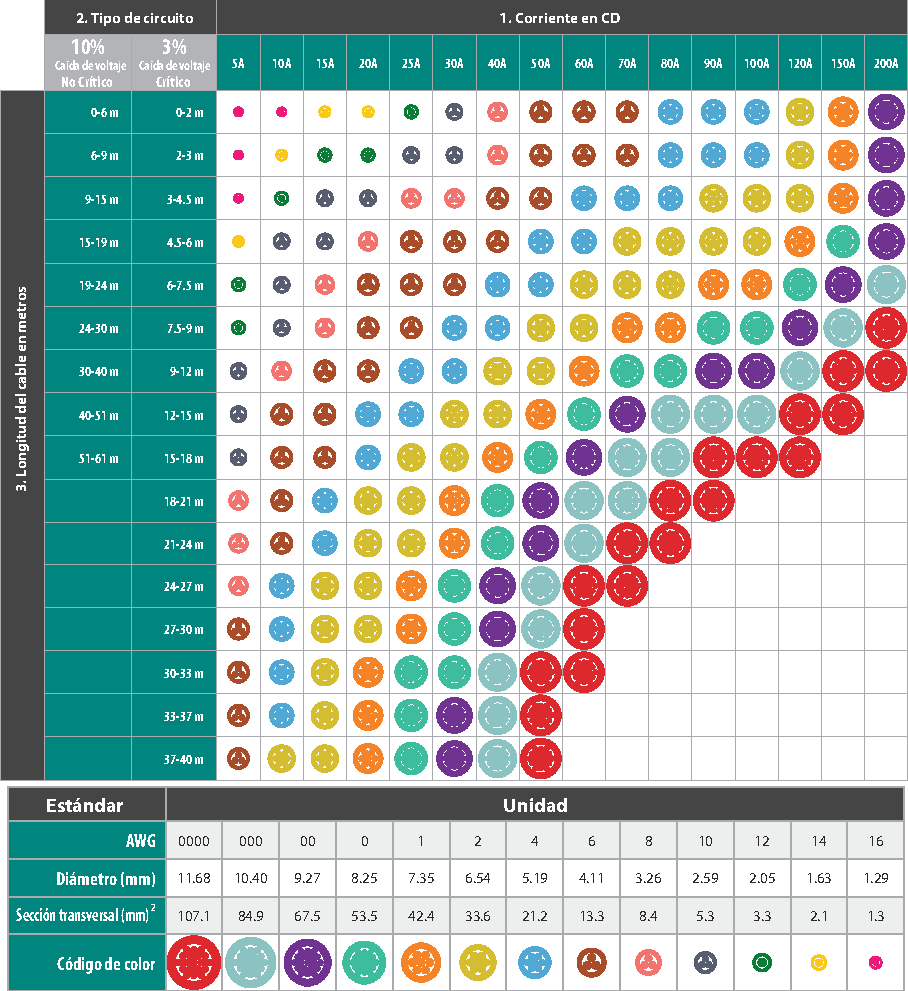
\includegraphics[scale=1]{imagenes/Marco Teorico/CalibreCable}
	\caption{Gu�a de selecci�n para calibre de cables, Blue Sea Systems}
	\label{fig:CableCalibre}
\end{figure}

\subsection{Visi�n artificial}

La visi�n por computadora es una de las herramientas m�s poderosas que existen en la actualidad para permitir a un robot identificar las condiciones del ambiente en el que opera.

Dos t�cnicas �tiles para obtener esto son la visi�n estereosc�pica, conocida como estereopsis, y la correcci�n de perspectiva, conocida como homograf�a.

\subsubsection*{Homograf�a}

Una homograf�a es una matriz que mapea las coordenadas de una imagen tomada en una perspectiva que no es normal a la superficie que se desea observar a una imagen no distorsionada con una perspectiva normal.

\begin{align}
\label{eq:Homografia}
\tilde{P}_{2} &\simeq H_{m}\tilde{P}_{1}
\end{align}

\begin{align*}
\textrm{En donde:}\\
\tilde{P}_{1} &= \textrm{Imagen original}\\
\tilde{P}_{2} &= \textrm{Imagen corregida}\\
H_{m} &= \textrm{Matriz de homograf�a}
\end{align*}

Por ejemplo, suponga que toma una foto de una catedral a nivel del suelo, lo cual resulta en una imagen distorsionada por la perspectiva, mostrada en la Figura \ref{fig:NuestraDonaPersp}.

Para corregirla, se seleccionan cuatro puntos de la imagen, como se muestra en el trapecio morado de coordenadas $X_{i},Y_{i}$ de la imagen. Este trapecio se mapea al rect�ngulo rojo con v�rtices en las coordenadas $x_{i},y_{i}$, resolviendo el sistema de ecuaciones  para obtener la matriz de homograf�a\cite{VISHUIT}.

\begin{align*}
\begin{bmatrix}
X_{1} & Y_{1} & 1 & 0 & 0 & 0 & -x_{1}X_{1} & -x_{1}Y_{1}\\
0 & 0 & 0 & X_{1} & Y_{1} & 1 & -y_{1}X_{1} & -y_{1}Y_{1}\\
X_{2} & Y_{2} & 1 & 0 & 0 & 0 & -x_{2}X_{2} & -x_{2}Y_{2}\\
0 & 0 & 0 & X_{2} & Y_{2} & 1 & -y_{2}X_{2} & -y_{2}Y_{2}\\
X_{3} & Y_{3} & 1 & 0 & 0 & 0 & -x_{3}X_{3} & -x_{3}Y_{3}\\
0 & 0 & 0 & X_{3} & Y_{3} & 1 & -y_{3}X_{3} & -y_{3}Y_{3}\\
X_{4} & Y_{4} & 1 & 0 & 0 & 0 & -x_{4}X_{4} & -x_{4}Y_{4}\\
0 & 0 & 0 & X_{4} & Y_{4} & 1 & -y_{4}X_{4} & -y_{4}Y_{4}\\
\end{bmatrix}
\begin{bmatrix}
h_{11}\\
h_{12}\\
h_{13}\\
h_{21}\\
h_{22}\\
h_{23}\\
h_{31}\\
h_{32}
\end{bmatrix}
=
\begin{bmatrix}
x_{1}\\
y_{1}\\
x_{2}\\
y_{2}\\
x_{3}\\
y_{3}\\
x_{4}\\
y_{4}
\end{bmatrix}
\end{align*}

La matriz $H_{m}$ es de la forma\footnote{El valor de $h_{33}$ se fija igual a 1 para que se pueda resolver el sistema de ecuaciones}

\begin{align*}
H_{m}=
\begin{bmatrix}
h_{11} & h_{12} & h_{13}\\
h_{21} & h_{22} & h_{23}\\
h_{31} & h_{32} & 1\\
\end{bmatrix}
\end{align*}

\begin{figure}
	\centering		
	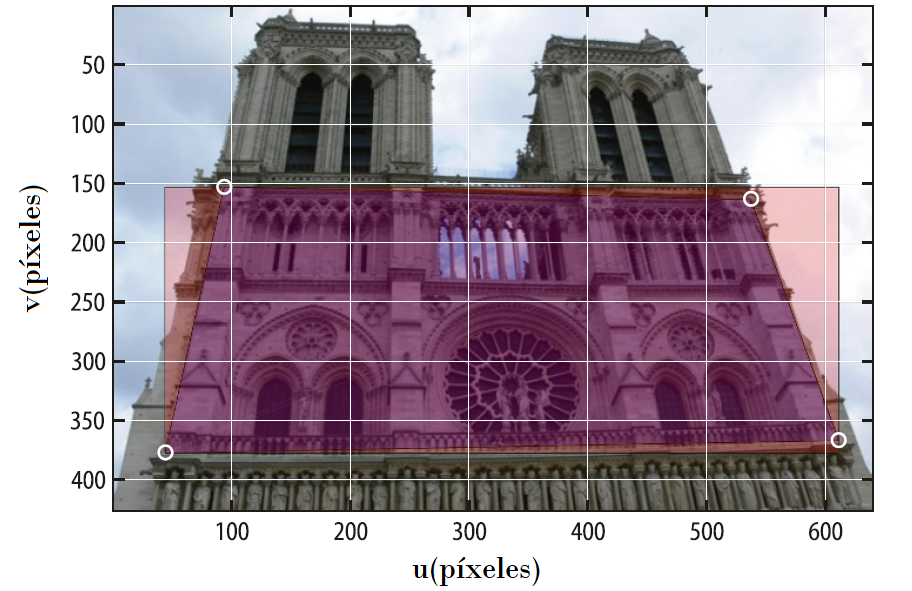
\includegraphics[scale=0.5]{imagenes/Marco Teorico/Robo1}
	\caption{Imagen original tomada en perspectiva}
	\label{fig:NuestraDonaPersp}
\end{figure}

\begin{figure}
	\centering		
	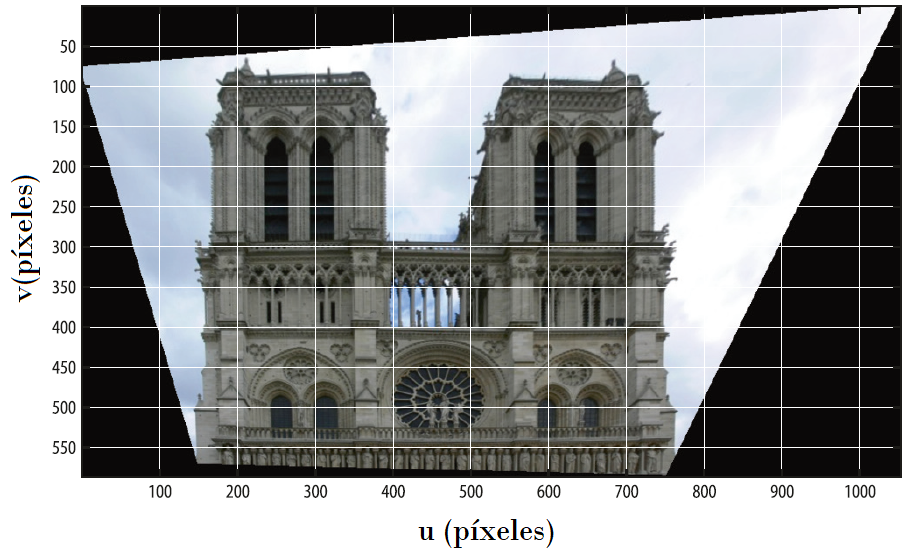
\includegraphics[scale=0.5]{imagenes/Marco Teorico/Robo2}
	\caption{Imagen corregida por la homograf�a}
	\label{fig:NuestraDonaChida}
\end{figure}

\begin{figure}
	\centering		
	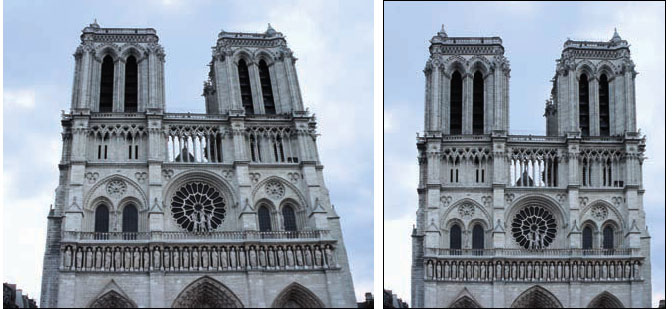
\includegraphics[scale=0.5]{imagenes/Marco Teorico/comparacionNuestraDona}
	\caption{Comparaci�n de la imagen original contra la corregida}
	\label{fig:NuestraDonaComp}
\end{figure}

\subsubsection*{Estereopsis}

La visi�n estereosc�pica implica tomar dos im�genes de un mismo objeto desde 2 puntos de vista distintos para estimar la distancia que hay entre las c�maras y el objeto. Normalmente se colocan dos c�maras iguales con sus ejes �pticos paralelos separados por una distancia conocida referida como l�nea base de las c�maras\cite{RoboCorke}.

\begin{figure}
	\centering		
	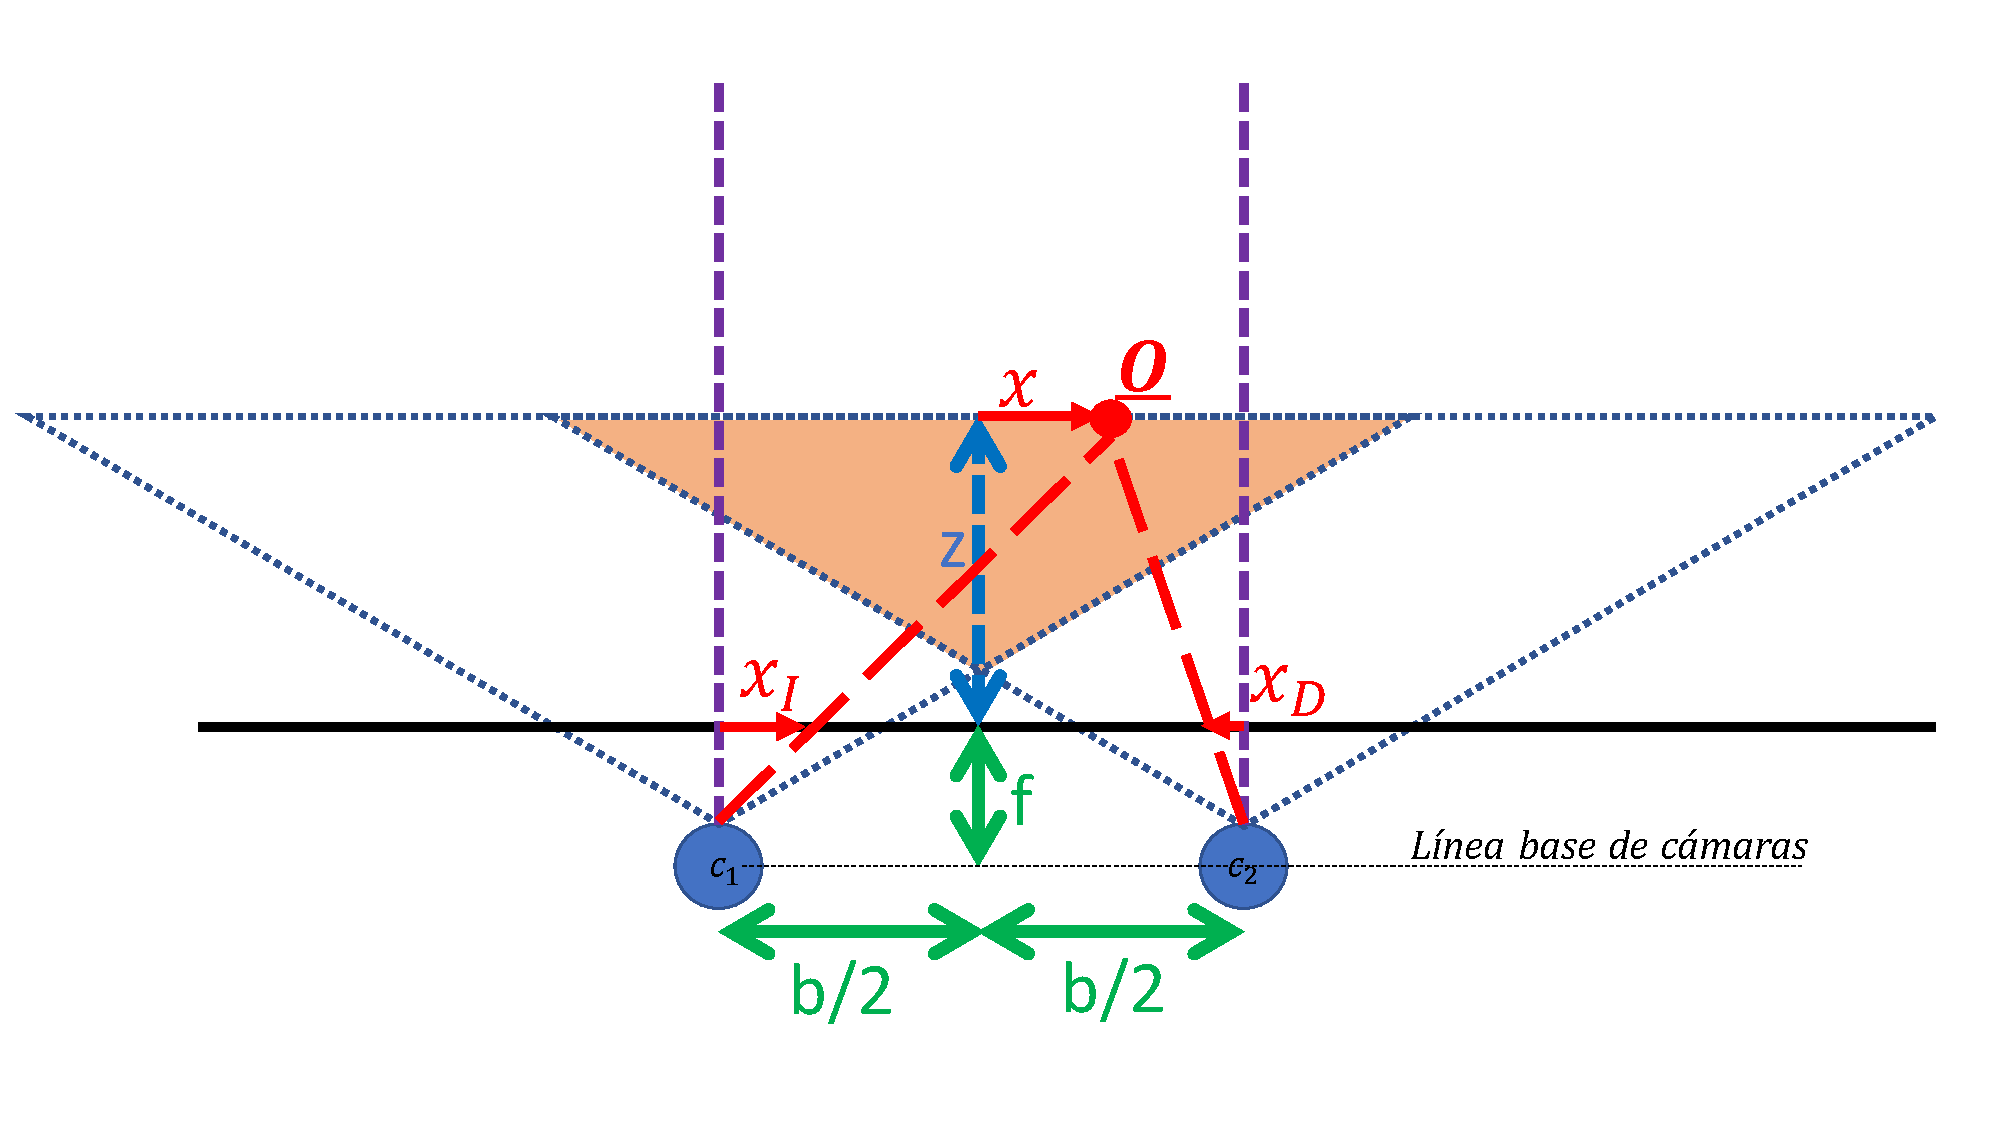
\includegraphics[scale=0.3]{imagenes/Dominio especifico/Informacion/Diagramas vision.pdf}
	\caption{Diagrama de referencia para la estereopsis}
	\label{fig:DiagramaEstereo}
\end{figure}

Con ayuda del diagrama mostrado en la Figura \ref{fig:DiagramaEstereo}, se calcula la profundidad como sigue:

Por tri�ngulos semejantes

\begin{align*}
\frac{x_{I}}{f} &= \frac{\frac{b}{2}+x}{z}\\
x_{I}&=f\left(\frac{\frac{b}{2}+x}{z}\right)\\
\frac{-x_{D}}{f} &= \frac{\frac{b}{2}-x}{z}\\
-x_{D}&=f\left(\frac{\frac{b}{2}-x}{z}\right)
\end{align*}

Luego

\begin{align*}
x_{I}-x_{D}&=\frac{fb}{z}
\end{align*}

\begin{align*}
z&=\frac{fb}{x_{I}-x_{D}}
\end{align*}

\begin{align*}
\textrm{En donde:}\\
x_{I}&=\textrm{\# de pixeles desde el origen hasta el} \\
&\textrm{centro del objeto en la imagen izquierda}\\
x_{D}&=\textrm{\# de pixeles desde el origen hasta el} \\
&\textrm{centro del objeto en la imagen derecha}\\
z&=\textrm{Profundidad}\\
b&=\textrm{Distancia entre c�maras}\\
x&=\textrm{Distancia real}
\end{align*}

\section{Marco procedimental}

\subsection{Metodolog�a mecatr�nica}
La metodolog�a de dise�o mecatr�nico que se utiliza es el modelo V, descrito en el est�ndar VDI 2206\cite{VDI2206}, el cual considera al proceso de dise�o como un
``macro-ciclo'' en el que el grado de madurez se incrementa con cada iteraci�n, y cuyo n�mero
de iteraciones depende del progreso realizado con cada una hasta llegar a un producto final
que cumpla satisfactoriamente con las expectativas de desempe�o esperadas.
Este modelo consta de 3 fases principales, denominadas \textbf{``Dise�o del sistema''}, la cual es la
fase inicial y comienza definiendo los requerimientos que el sistema debe satisfacer, seguido
de la descomposici�n de las funciones que lleva a cabo, para poder dar paso a la fase de
\textbf{``Dise�o de dominio espec�fico''}, en el que se realiza un dise�o a profundidad de cada una
de las disciplinas involucradas, para llegar finalmente a la \textbf{``Integraci�n del sistema''}, en
donde se implementan todos los m�dulos y se unen para trabajar arm�nicamente.
Adem�s de las fases principales, el modelo cuenta con 2 fases que son transversales a todo
el proceso, las cuales son el \textbf{``Modelado y an�lisis del modelo''}, en la cual se realizan
modelos que describen el comportamiento de cada uno de los m�dulos y del sistema en
general, para poder realizar simulaciones que ayudan en la fase de \textbf{``Validaci�n y
verificaci�n''}, la cual se realiza en todo momento para evaluar el desempe�o de cada
m�dulo y determinar el grado de madurez del proyecto.

\begin{figure}
	\centering		
	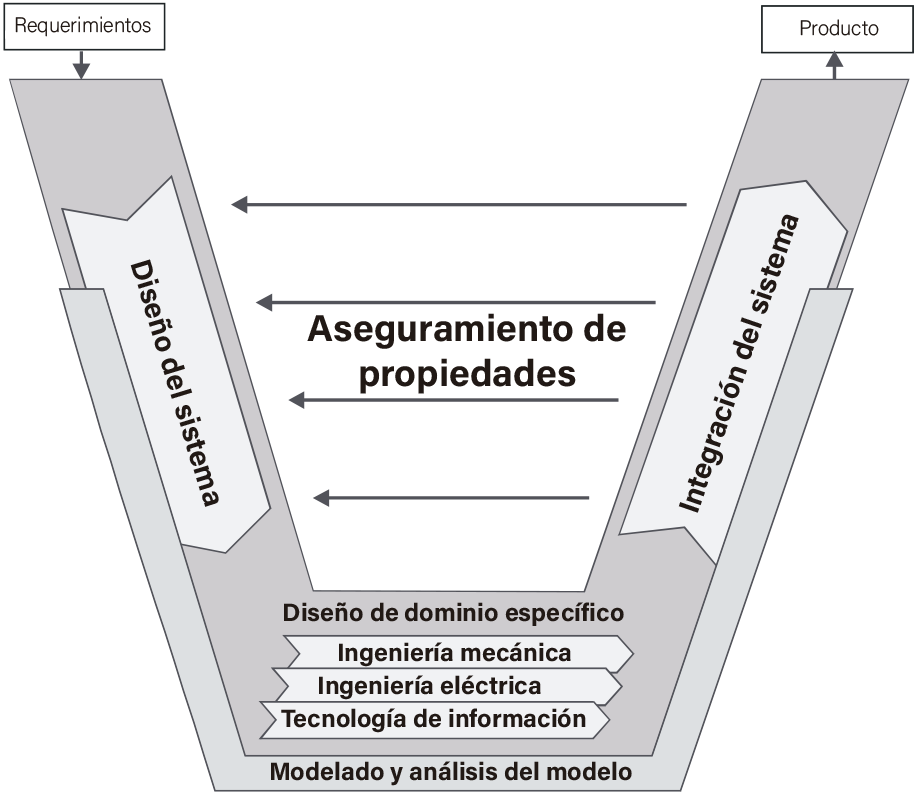
\includegraphics[scale=1.3]{imagenes/VDI2206}
	\caption{Modelo V como metodolog�a para el dise�o mecatr�nico(VDI 2206)}
	\label{fig:VDI2206}
\end{figure}

\pagebreak
%\pagediagram
%%%%%%%%%%%%%%%%%%%%%%%%%%%%%%%%%%%%%%%%%%%%%%%%%%%%%%%%%%%%%%%%%%%
%%%%%%%%%%%%%%%%%%%%%%%%%%%%%%%%%%%%%%%%%%%%%%%%%%%%%%%%%%%%%%%%%%%
% !TeX encoding = ISO-8859-1
\chapter{Dise�o}

\section{Dise�o del sistema}

A lo largo de este cap�tulo se establecen las necesidades que el sistema mecatr�nico debe satisfacer, para posteriormente determinar las funciones a realizar y los m�dulos que forman parte del concepto de soluci�n, el cual se elige a trav�s de la implementaci�n de una herramienta de selecci�n multicriterio.

\subsection{Necesidades y requerimientos}

Para dar comienzo con el dise�o del sistema, es preciso determinar cuales son las \textbf{necesidades}\cite{Trazabilidad} que debe satisfacer, las cuales son el resultado de la \textit{transformaci�n} de uno o m�s conceptos en una \textit{expectativa} para el cumplimiento de una \textit{funci�n} de acuerdo a ciertos indicadores de \textit{rendimiento} que aseguren la \textit{calidad}. La Tabla \ref{Tabla:TabNec} asocia las necesidades establecidas con un identficador, el cual ser� �til para identificarlas r�pidamente a lo largo del proceso de dise�o. 

\begin{table}
\centering
\caption{Necesidades que el sistema debe cumplir}
\begin{scriptsize}
\begin{tabular}{|c|c|}
\hline
\textbf{Identificador} & \textbf{Necesidad}                                                                                                          \\ \hline
N1                     & Tomar la muestra desde su posici�n de origen.                                                                               \\ \hline
N2                     & \begin{tabular}[c]{@{}c@{}}Ser capaz de trabajar en las condiciones ambientales determinadas para la\\ misi�n.\end{tabular} \\ \hline
N3                     & Obtener datos de la muestra.                                                                                                \\ \hline
N4                     & Enviar datos.                                                                                                               \\ \hline
N5                     & Recibir instrucciones.                                                                                                      \\ \hline
N6                     & Ser ligero.                                                                                                                 \\ \hline
N7                     & No desequilibrar al \textit{rover}.                                                                                                  \\ \hline
N8                     & Tener dimensiones reducidas.                                                                                                \\ \hline
N9                     & Trabajar bajo el sol.                                                                                                       \\ \hline
N10                    & Consumir poca energ�a.                                                                                                      \\ \hline
\end{tabular}
\end{scriptsize}
\label{Tabla:TabNec}
\end{table}

Una vez que se han establecido las necesidades que el sistema debe satisfacer, es posible establecer los \textbf{requerimientos}\cite{Trazabilidad} t�cnicos que  componen las espeficaciones del mismo, pues estos son el resultado de transformar las necesidades en una obligaci�n para cumplir cierta funci�n dentro de las cotas establecidas, de manera an�loga a la tabla de necesidades (Tabla \ref{Tabla:TabNec}), la Tabla \ref{Tabla:TabReq} asocia cada requerimiento con un identificador.

\begin{table}
\centering
\caption{Requerimientos t�cnicos del sistema}
\begin{scriptsize}
\begin{tabular}{|c|c|c|}
\hline
\textbf{Identificador} & \textbf{Requerimiento}               & \textbf{Valor}                   \\ \hline
R1                     & Masa m�xima de la muestra            & 100 g                            \\ \hline
R2                     & Di�metro m�ximo de la muestra        & 5 cm                             \\ \hline
R3                     & Esfericidad                          & Media a alta                     \\ \hline
R4                     & Angularidad     & Sub-angular a bien redondeada    \\ \hline
R5                     & Masa m�xima del sistema              & 12 kg                            \\ \hline
R6                     & Envergadura m�xima                   & 1.5 m                            \\ \hline
R7                     & Alimentaci�n m�xima                         & 24 V                        \\ \hline
R8                     & Resoluci�n m�nima de masa de muestra & 1 g                              \\ \hline
R9                     & Rango de comunicaci�n                & Entre 2 y 10 m                   \\ \hline
R10                    & �rea de recolecci�n                  & $1m^{2}$                         \\ \hline
R11                    & Temperatura de trabajo               & $5^{\circ}C<t_{amb}<25^{\circ}C$ \\ \hline
R12                    & Humedad del ambiente                 & $20\%<h_{amb}<70\%)$             \\ \hline
R13                    & Tiempo de ciclos de operaci�n & 10 min                           \\ \hline
\end{tabular}
\end{scriptsize}
\label{Tabla:TabReq}
\end{table}

\subsubsection*{Validaci�n de requerimientos}
Para evaluar si los requerimientos cubren todas las necesidades establecidas, se utiliza la matriz de trazabilidad\cite{Trazabilidad}.

La Tabla \ref{Tabla:TrazaReq} contiene las necesidades en las columnas y las filas representan los requerimientos derivados. Con el fin de comprobar que todas las necesidades se satisface, es importante que cada una est� asociada al menos a un requerimiento.

Para llevar la muestra de su lugar de origen al lugar de an�lisis (N1), es necesario tomar en cuenta las caracter�sticas f�sicas de la misma, como son, masa(R1), di�metro (R2), esfericidad\cite{Esfericidad}(R3), angularidad\cite{Esfericidad}(R4), adem�s de la destreza del sistema (R6 y R10).

Para asegurar que el sistema es capaz de trabajar en el ambiente determinado (N2), se deben conocer la temperatura y humedad del mismo (R11 y R12), as� como el tiempo de operaci�n (R13).

Debido a que el sistema est� dise�ado para analizar piedras peque�as (N3), es necesario que sea capaz de medir la masa de manera precisa (R8).

Para que el sistema sea capaz de trabajar de manera remota (N4 y N5), es necesario establecer cotas de distancia (R9).

La necesidad 6 se asocia directamente con un l�mite de masa (R5).

Los l�mites de masa y dimensiones (R5 y R6) garantizan que las reacciones generadas no vuelquen al ``\textit{rover}''(N7).

La necesidad 8 se asocia directamente con un l�mite de longitud (R6).

El sistema debe ser capaz de trabajar en las condiciones t�picas (R11 y R12) de un ambiente a la intemperie (N9).

Para asegurar un bajo consumo de energ�a, se deben establecer l�mites a la masa de la muestra a tomar (R1), el peso propio del sistema (R5), las dimensiones del manipulador (R6), la energ�a disponible (R7), y el tiempo en que se puede operar(R13).

\begin{table}
\centering
\caption{Matriz de trazabilidad para la validaci�n de requerimientos respecto a necesidades}
\begin{scriptsize}
\begin{tabular}{c|c|c|c|c|c|c|c|c|c|c|}
\cline{2-11}
                          & N1                    & N2                              & N3                    & N4                    & N5                    & N6                    & N7                    & N8                    & N9                    & N10        \\ \hline
\multicolumn{1}{|c|}{R1}  &\Checkmark            &                                 &                       &                       &                       &                       &                       &                       &                       & \Checkmark \\ \hline
\multicolumn{1}{|c|}{R2}  & \Checkmark            &                                 &                       &                       &                       &                       &                       &                       &                       &            \\ \hline
\multicolumn{1}{|c|}{R3}  & \Checkmark            &                                 &                       &                       &                       &                       &                       &                       &                       &            \\ \hline
\multicolumn{1}{|c|}{R4}  & \Checkmark            &                                 &                       &                       &                       &                       &                       &                       &                       &            \\ \hline
\multicolumn{1}{|c|}{R5}  &                       &                                 &                       &                       &                       & \Checkmark            & \Checkmark            &                       &                       & \Checkmark \\ \hline
\multicolumn{1}{|c|}{R6}  & \Checkmark            &                                 &                       &                       &                       &                       & \Checkmark            & \Checkmark            &                       & \Checkmark \\ \hline
\multicolumn{1}{|c|}{R7}  &                       &                                 &                       &                       &                       &                       &                       &                       &                       & \Checkmark \\ \hline
\multicolumn{1}{|c|}{R8}  &                       &                                 & \Checkmark            &                       &                       &                       &                       &                       &                       &            \\ \hline
\multicolumn{1}{|c|}{R9}  &                       &                                 &                       & \Checkmark            & \Checkmark            &                       &                       &                       &                       &            \\ \hline
\multicolumn{1}{|c|}{R10} & \Checkmark            &                                 &                       &                       &                       &                       &                       &                       &                       &            \\ \hline
\multicolumn{1}{|c|}{R11} &                       & \Checkmark                      &                       &                       &                       &                       &                       &                       & \Checkmark            &            \\ \hline
\multicolumn{1}{|c|}{R12} &                       & \Checkmark                      &                       &                       &                       &                       &                       &                       &                       &            \\ \hline
\multicolumn{1}{|c|}{R13} & \multicolumn{1}{c|}{} & \multicolumn{1}{c|}{\Checkmark} & \multicolumn{1}{c|}{} & \multicolumn{1}{c|}{} & \multicolumn{1}{c|}{} & \multicolumn{1}{c|}{} & \multicolumn{1}{c|}{} & \multicolumn{1}{c|}{} & \multicolumn{1}{c|}{} & \Checkmark \\ \hline
\end{tabular}
\end{scriptsize}
\label{Tabla:TrazaReq}
\end{table}

\subsection{Arquitectura funcional}

En esta secci�n se lleva a cabo la descomposici�n de \textbf{funciones}, dividiendo la funci�n general, la cual describe el comportamiento del sistema, en funciones secundarias inherentes al mismo, as� como las funciones gen�ricas, que pueden asociarse a la mayor�a de sistemas.

Una vez que se han determinado los requerimientos principales, es posible establecer la funci�n general, cuyo objetivo es describir el funcionamiento que tiene
el sistema; posteriormente, se debe realizar una descomposici�n de la funci�n principal en subfunciones que realicen una tarea en espec�fico
a modo de que sea m�s sencillo comprender los problemas a los que el dise�ador debe
enfrentarse.
Una forma de realizar esta descomposici�n es utilizar una herramienta denominada FBS\cite{FBS}
(\textit{Functional Breakdown Structure} por sus siglas en ingl�s), mostrada en la Figura \ref{fig:FBS}, la cual permite ver las funciones que desempe�a el sistema de una manera organizada y jer�rquica, las cuales se enlistan a continuaci�n.

\begin{figure}
	\centering		
	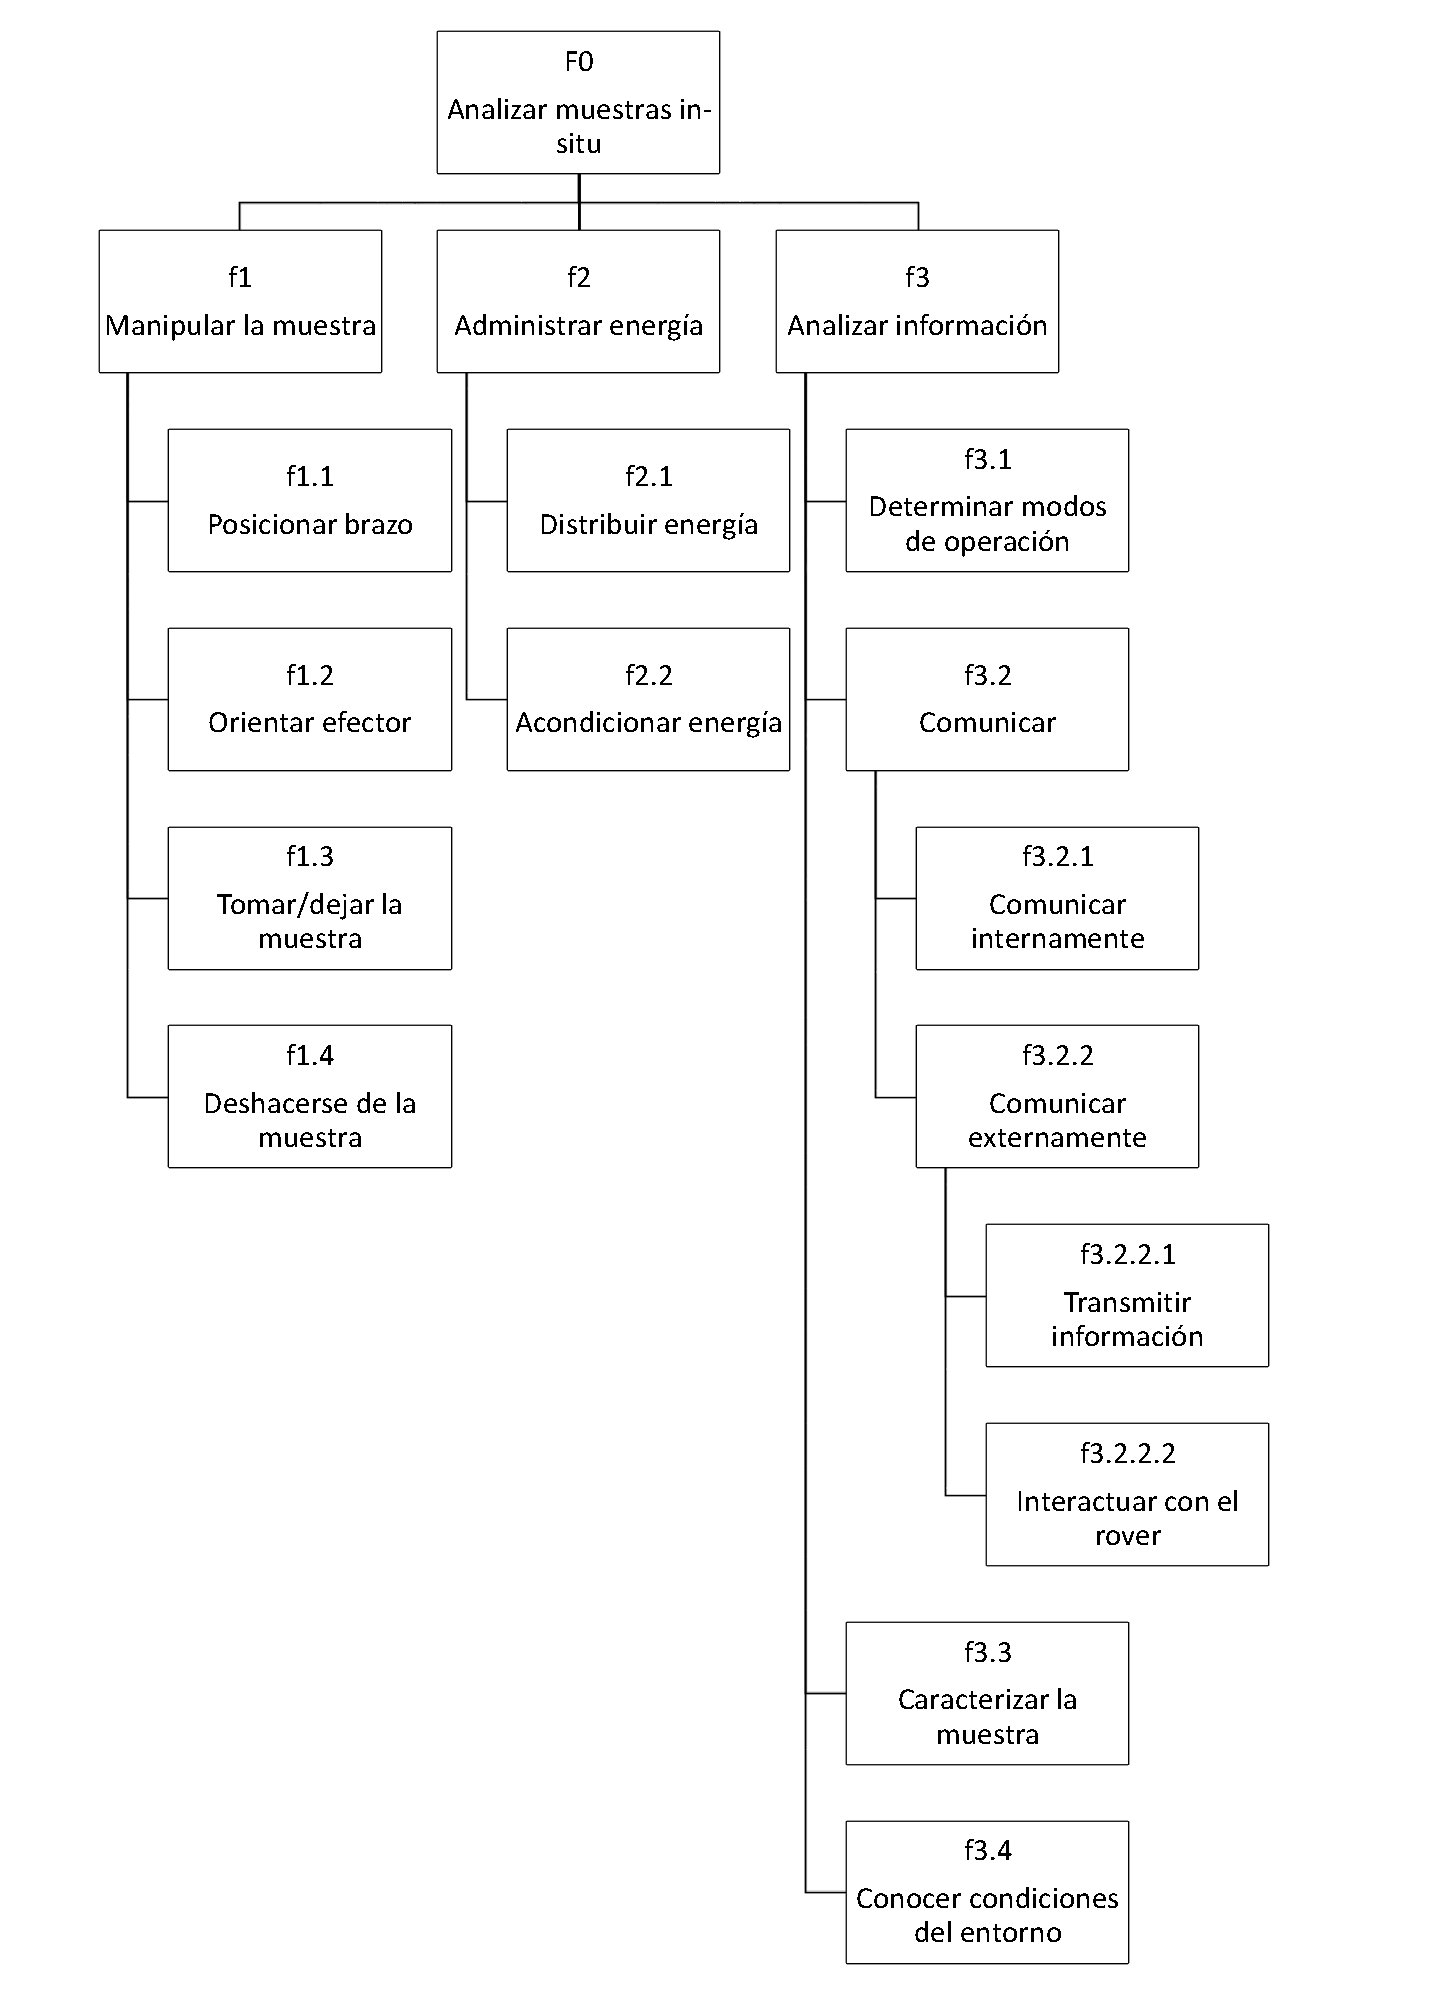
\includegraphics[scale=0.55]{imagenes/Modelos/FBS.pdf}
	\caption{Desglose gr�fico de funciones a trav�s de un modelo FBS}
	\label{fig:FBS}
\end{figure}


\subsubsection*{Validaci�n de funciones}
La Tabla \ref{Tabla:TrazaFun} muestra las relaciones existentes entre las funciones y los requerimientos.

Para el traslado de una muestra con las caracter�sticas especificadas en los requerimientos R1, R2, R3 y R4, es necesario que el sistema se posicione y oriente de manera que pueda tomar la muestra de su origen (f1.1 y f1.2), y posteriormente depositarla en el �rea de an�lisis (f1.3). Una vez que hayan obtenido los datos de la misma (f3.3), sea devuelta al entorno (f1.4).

En general, es deseable que un sistema gaste la menor cantidad de energ�a posible (f2.1), siendo la reducci�n del peso una forma de conseguirlo (R5).

Las funciones de posicionamiento y orientaci�n (f1.1 y f1.2) son realizadas dentro de las cotas establecidas en los requerimientos R6 y R10, que hablan sobre el alcance m�ximo del brazo y el �rea de recolecci�n respectivamente,  el cual recibe las coordenadas del objetivo mediante el sistema de percepci�n (f3.4).

Para cumplir con la funci�n general, utilizando la energ�a disponible descrita en el requerimiento R7, son implementadas las funciones de gesti�n energ�tica (f2.1 y f2.2), as� como la toma de decisiones basada en el nivel de energ�a disponible (f3.1), el cual se toma del sistema energ�tico general que incluye al rover (f3.2.2.2).

Para obtener una medici�n confiable de la muestra (R8), es necesario contar con un sistema de medici�n adecuado (f3.3).

Una comunicaci�n remota(R9) se consigue al transmitir datos de manera bidireccional entre el usuario y el sistema (f3.2.2.1), los cuales se encuentran alejados uno del otro.

El �rea de recolecci�n (R10) es aquella definida por los puntos en el espacio que el sistema puede alcanzar mediante las operaciones de posici�n y orientaci�n del manipulador (f1.1 y f1.2).

Para determinar los modos de operaci�n (f3.1), es necesario que el sistema obtenga los par�metros del entorno (R11 y R12) mediante un sistema de percepci�n (f3.4), el cual comunicar� los datos obtenidos (f3.2.1).

Conocer el nivel de energ�a disponible (f3.2.1), permite saber si es posible realizar la funci�n general (f2.1 y f3.1) para que, en caso negativo, se notifique al usuario (f3.2.2.1).

\begin{table}
\centering
\caption{Matriz de trazabilidad para la validaci�n de funciones respecto a requerimientos}
\begin{scriptsize}
\begin{tabular}{c|c|c|c|c|c|c|c|c|c|c|c|c|c|}
\cline{2-14}
                           	& \multicolumn{1}{c|}{R1} & \multicolumn{1}{c|}{R2} & \multicolumn{1}{c|}{R3} & \multicolumn{1}{c|}{R4} & \multicolumn{1}{c|}{R5} & \multicolumn{1}{c|}{R6} & \multicolumn{1}{c|}{R7} & \multicolumn{1}{c|}{R8} & \multicolumn{1}{c|}{R9} & \multicolumn{1}{c|}{R10} & \multicolumn{1}{c|}{R11} & \multicolumn{1}{c|}{R12} & R13 \\ \hline
\multicolumn{1}{|c|}{f1.1} 	& \Checkmark                  	&                     	&                     	&                     	&                     	& \Checkmark                   	&                     	&                     	&                     	& \Checkmark                    	&                      	&                      	& 	\\ \hline
\multicolumn{1}{|c|}{f1.2} 	& \Checkmark                    	&                     	&                     	&                     	&                     	& \Checkmark                   	&                     	&                     	&                     	& \Checkmark                   	&                      	&                      	& 	\\ \hline
\multicolumn{1}{|c|}{f1.3} 	& \Checkmark                   	& \Checkmark                   	& \Checkmark                   	& \Checkmark                   	&                     	&                     	&                     	&                     	&                     	&                      	&                      	&                      	& 	\\ \hline
\multicolumn{1}{|c|}{f1.4} 	& \Checkmark                   	& \Checkmark                   	& \Checkmark                   	& \Checkmark                   	&                     	&                     	&                     	&                     	&                     	&                      	&                      	&                      	& 	\\ \hline
\multicolumn{1}{|c|}{f2.1} 	&                     	&                     	&                     	&                     	&        \Checkmark             	&                     	& \Checkmark                  	&                     	&                     	&                      	&                      	&                      	& \Checkmark   \\ \hline
\multicolumn{1}{|c|}{f2.2} 	&                     	&                     	&                     	&                     	&                     	&                     	& \Checkmark                   	&                     	&                     	&                      	&                      	&                      	& 	\\ \hline
\multicolumn{1}{|c|}{f3.1} 	&                     	&                    	&                     	&                     	&                     	&                     	& \Checkmark                   	&                     	&                     	&                      	& \Checkmark                    	& \Checkmark                    	& \Checkmark   \\ \hline
\multicolumn{1}{|c|}{f3.2.1}   &                     	&                     	&                     	&                     	&                     	&                     	&                     	&                     	&                     	&                      	& \Checkmark                    	& \Checkmark                    	& \Checkmark   \\ \hline
\multicolumn{1}{|c|}{f3.2.2.1} &                     	&                     	&                     	&                     	&                     	&                     	&                     	&                     	& \Checkmark                   	&                      	&                      	&                      	&\Checkmark   \\ \hline
\multicolumn{1}{|c|}{f3.2.2.2} &                     	&                     	&                     	&                     	&                     	&                     	& \Checkmark                   	&                     	&                     	&                      	&                      	&                      	& 	\\ \hline
\multicolumn{1}{|c|}{f3.3} 	&   \Checkmark                  	& \Checkmark                   	& \Checkmark                   	& \Checkmark                   	&  	&                     	&                     	& \Checkmark                   	&                     	&                      	&                      	&                      	& 	\\ \hline
\multicolumn{1}{|c|}{f3.4} 	& \multicolumn{1}{c|}{}   & \multicolumn{1}{c|}{}   & \multicolumn{1}{c|}{}   & \multicolumn{1}{c|}{}   & \multicolumn{1}{c|}{}   & \multicolumn{1}{c|}{}   & \multicolumn{1}{c|}{}   & \multicolumn{1}{c|}{}   & \multicolumn{1}{c|}{}   & \multicolumn{1}{c|}{\Checkmark}   & \multicolumn{1}{c|}{\Checkmark}   & \multicolumn{1}{c|}{\Checkmark}   & 	\\ \hline
\end{tabular}
\end{scriptsize}
\label{Tabla:TrazaFun}
\end{table}

Una vez que se han determinado las funciones que desempe�a el sistema, es posible
definir los \textbf{m�dulos} que lo componen, con el objetivo de dar soluci�n a problemas
espec�ficos. Para ello resulta �til determinar la relaci�n existente entre las mismas a trav�s del modelo IDEF-0\cite{IDEF0}. El modelo del nodo A0 expandido, mostrado en la Figura \ref{fig:IDEF0A0E} permite dimensionar la complejidad del proyecto, facilitando la comprensi�n del comportamiento del sistema y por ende, la b�squeda de posibles soluciones. 


\begin{landscape}
	\begin{figure}[p]
		\centering		
		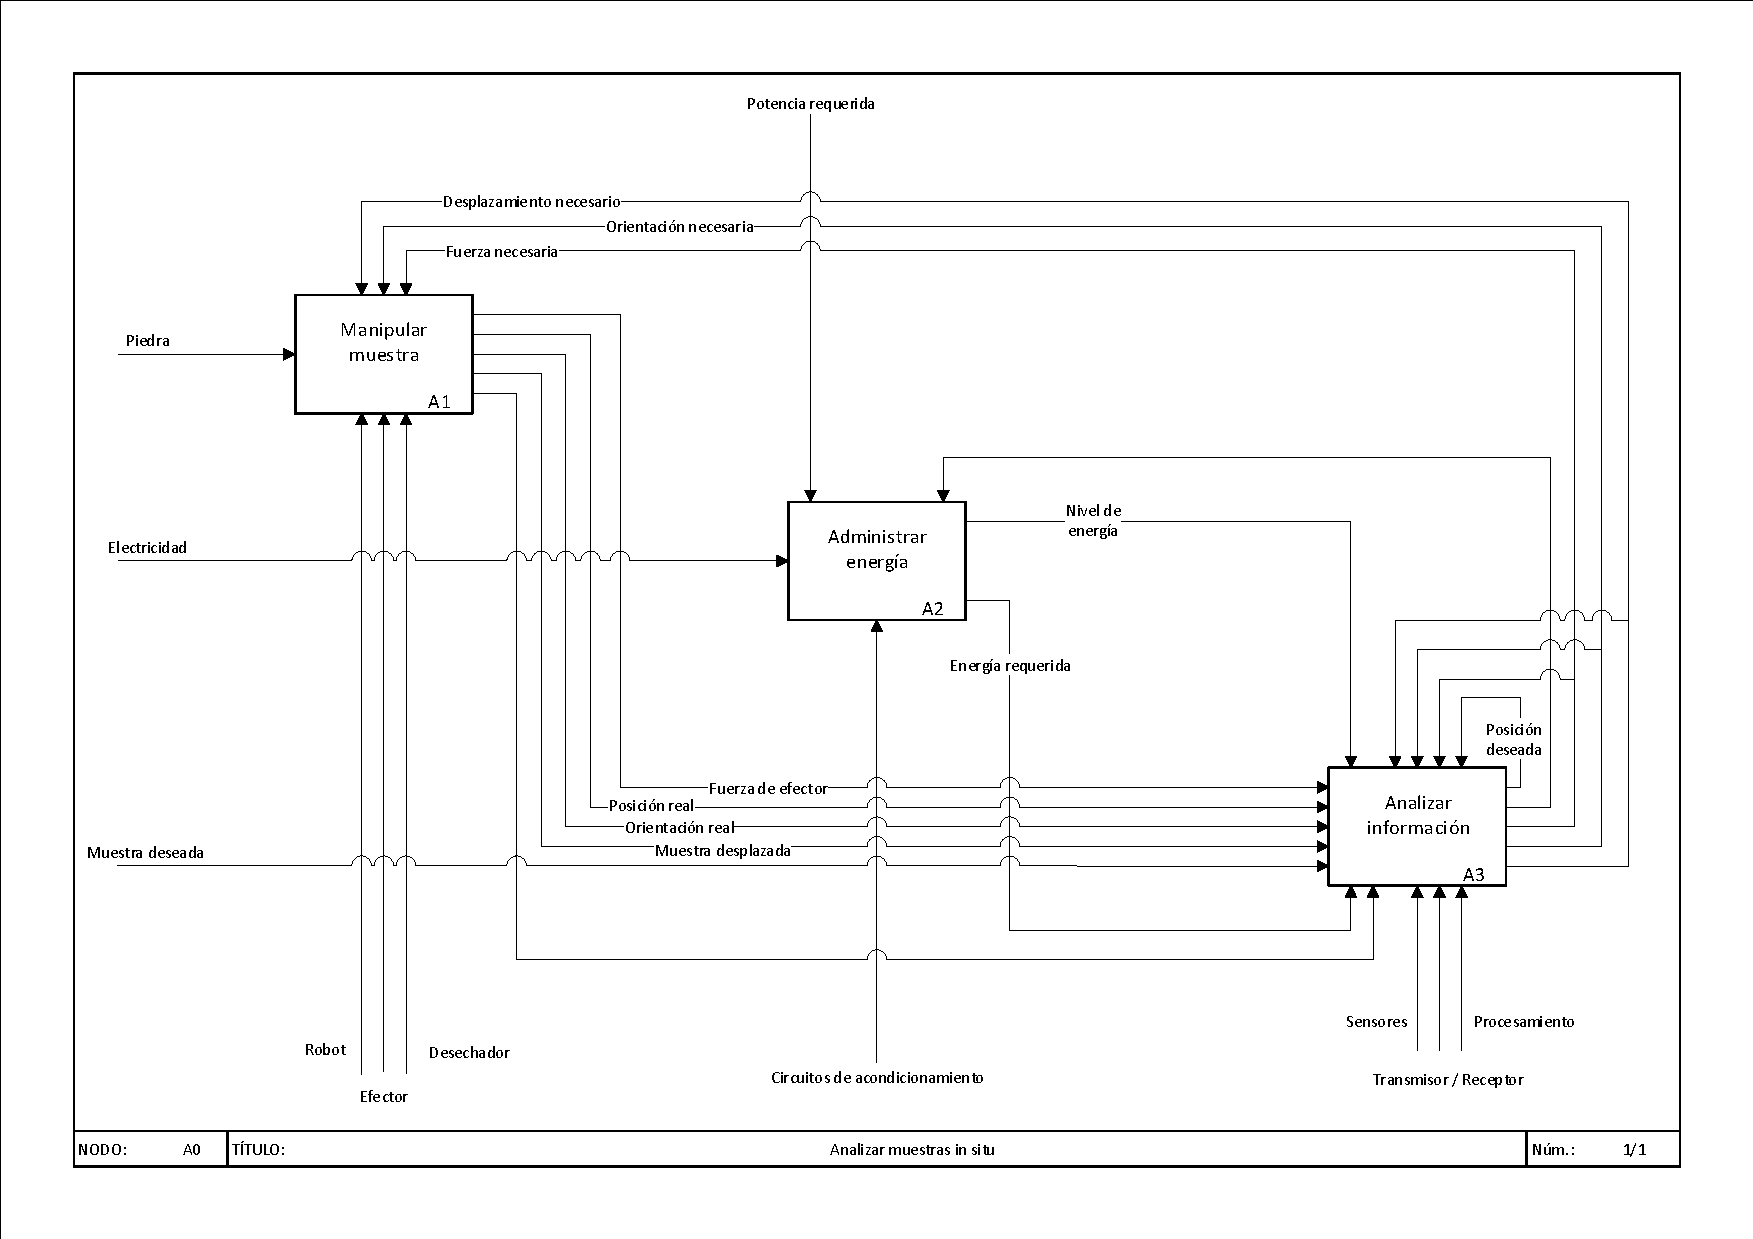
\includegraphics[width=1.5\textwidth ,height=\textheight, trim=4 4 4 4,clip]{imagenes/Modelos/IDEF0.pdf}
		\caption{Modelo IDEF0 del sistema}
		\label{fig:IDEF0A0E}
	\end{figure}
\end{landscape}


As� mismo, resulta de gran utilidad analizar el comportamiento del sistema mediante la ejecuci�n de las funciones. Esto permite observar como cada funci�n contribuye al cumplimiento de la funci�n principal del sistema y como se relacionan entre si, identificando las condiciones que cada una necesita para ejecutarse, mostrando la interacci�n entre las entradas y salidas a lo largo de las transformaciones realizadas. 
Para ello se utiliza el modelo mostrado en la Figura \ref{fig:eFFBD}, el cual es un diagrama a bloques mejorado del flujo de funciones (\textit{eFFBD - enhanced Function Flow Block Diagram} por sus siglas en ingl�s)\cite{eFFBD}. Este modelo permite observar que la comunicaci�n y la administraci�n energ�tica permanecen activas hasta que el sistema sea desactivado, mientras que para que se realice la funci�n general, es necesario que el usuario lo ordene, pues de lo contrario el proceso nunca dar� inicio. Por otro lado, el sistema eval�a las condiciones de trabajo actuales, tanto externas como internas, y con base en ellas decide la acci�n a realizar, ya sea quedarse en la posici�n de reposo o la toma de la muestra, cuyo proceso se realiza a trav�s del posicionamiento y orientaci�n del sistema rob�tico hacia la ubicaci�n de la muestra en el entorno, seguido del traslado al laboratorio, el cual, tras obtener informaci�n de ella la devuelve al ambiente.


\begin{landscape}
	\begin{figure}[p]
		\centering		
		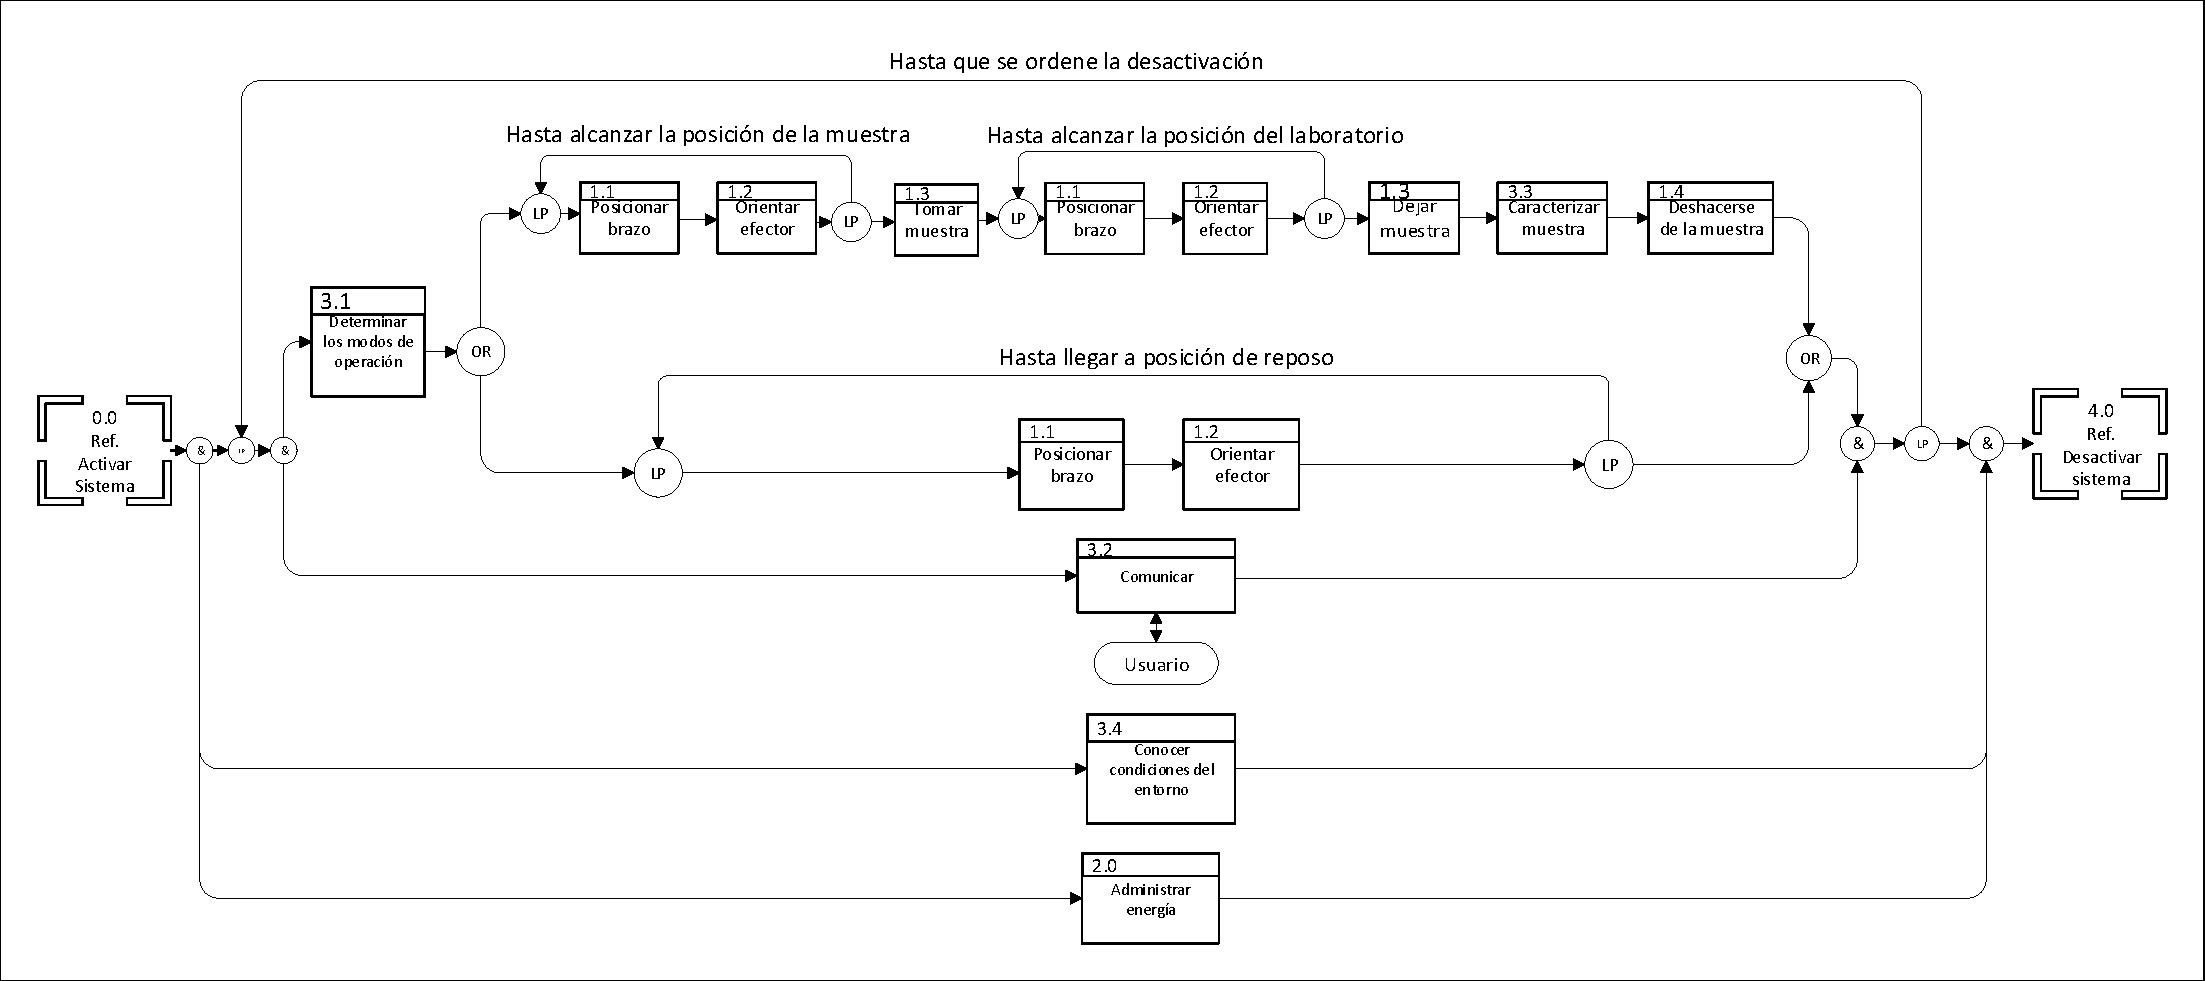
\includegraphics[width=1.55\textwidth ,height=0.85\textheight, trim=4 4 4 4,clip]{imagenes/Modelos/eFFBD.pdf}
		\caption{Modelo mejorado del diagrama a bloques de flujo funcional}
		\label{fig:eFFBD}
	\end{figure}
\end{landscape}


\subsection{Arquitectura f�sica}

Una vez que se ha analizado el comportamiento del sistema mediante las funciones y la relaci�n existente entre ellas, es posible deducir los elementos f�sicos que las lleven a cabo, los cuales pueden agruparse en los siguientes sistemas con sus correspondientes m�dulos.

\begin{itemize}
\item[S1] Rob�tico.
	\begin{itemize}[noitemsep,nolistsep]
	\item[M1] Manipulador: Un brazo de 3 grados de libertad (GDL) m�s una mu�eca esf�rica de 3 GDL que realizar� la funci�n de posicionar y orientar al efector final, con el objetivo de trasladar la muestra.
	\item[M2] Efector final: Herramienta colocada en el extremo del manipulador capaz de sujetar la muestra.
	\end{itemize}

\item[S2] Informaci�n
	\begin{itemize}[noitemsep,nolistsep]
	\item[M3] Percepci�n: Sensores que le permitir�n al sistema obtener informaci�n de s� mismo y de su entorno con el fin de conocer los par�metros necesarios para tomar decisiones.
	\item[M4] Comunicaci�n: Elementos que permitan realizar la transmisi�n y recepci�n de informaci�n.
	\item[M5] Procesamiento: Componentes electr�nicos que permitan analizar la informaci�n, tomar decisiones y enviar �rdenes.
	\end{itemize}
\item[S3] Administraci�n energ�tica: Fuente de alimentaci�n y circuitos que adapten la energ�a de acuerdo a las necesidades de cada componente.
\item[S4] Laboratorio
	\begin{itemize}[noitemsep,nolistsep]
	\item[M6] Obtenci�n de datos de la muestra: Sensores que le permitir�n al sistema obtener informaci�n de la muestra de inter�s.
	\item[M7] Desechador: Mecanismo encargado de expulsar la muestra del sistema.
	\end{itemize}
\item[S5] Estructural: Soporte y protecci�n para los componentes que conforman el sistema.
\end{itemize}

\subsubsection*{Validaci�n de m�dulos}

La Tabla \ref{Tabla:TrazaMod} muestra la matriz de trazabilidad utilizada para validar los m�dulos propuestos al comprobar que cada una de las funciones es realizada por alg�n m�dulo, y que cada m�dulo cumple al menos una funci�n.

En primer lugar, se puede apreciar f�cilmente que S3 y S5 est�n presentes en todas las funciones, pues para que sean realizadas, es fundamental que cuenten con la energ�a necesaria, adem�s de que el sistema debe ensamblarse de manera integral.

Las funciones de posicionamiento y orientaci�n(f1.1 y f1.2) se llevan a cabo a trav�s del manipulador M1, el cual recibe las coordenadas del objetivo en el espacio tridimensional mediante M3, el cual env�a los datos a M5 para que haga los c�lculos necesarios de cinem�tica inversa y control.

El efector final M2 toma la muestra de su posici�n original y la deposita en el �rea de an�lisis (f1.3), mediante las funciones de posicionamiento y orientaci�n (f1.1 y f1.2).

La muestra se devuelve al entorno (f1.4) mediante M7, el cual es controlado por M5.

Para seleccionar el modo de operaci�n (f3.1), se utiliza la informaci�n provista por M3 sobre la condiciones del ambiente, y M5 sobre la energ�a disponible.

Para que el sistema pueda realizar la funci�n general, es necesario que haya comunicaci�n (M4) entre todos sus sistemas y m�dulos (f3.2.1), para que se puedan realizar las tomas de decisiones, y adem�s, informar al usuario(f3.2.2.1) sobre los datos obtenidos (M6) y los problemas que se presenten (M3).	

La interacci�n con el rover (f3.2.2.2) se realiza mediante M4, para recibir de �ste el nivel de energ�a disponible.

Los datos f�sicos de la muestra se obtienen (f3.3) a trav�s de M6, y su posici�n a trav�s de M3. 

Las condiciones del entorno se obtienen a trav�s de M3.

\begin{table}
\centering
\caption{Matriz de trazabilidad para la validaci�n de m�dulos respecto a funciones}
\begin{scriptsize}
\begin{tabular}{c|c|c|c|c|c|c|c|c|c|c|c|c|}
\cline{2-13}
                     	& f1.1                                       	& f1.2                                       	& f1.3                                       	& f1.4                                       	& f2.1                                       	& f2.2                                       	& f3.1                                       	& f3.2.1                                     	& f3.2.2.1                                   	& f.3.2.2                                    	& f3.3                                       	& f3.4                                       	\\ \hline
\multicolumn{1}{|c|}{M1} & \Checkmark                  	&                                            	& \Checkmark                  	&                                            	&                                            	&                                            	&                   	&                                            	&                                            	&                                            	&                                            	&                                            	\\ \hline
\multicolumn{1}{|c|}{M2} &                                            	& \Checkmark                  	& \Checkmark                  	&                                            	&                                            	&                                            	&                 	&                                            	&                                            	&                                            	&                                            	&                                            	\\ \hline
\multicolumn{1}{|c|}{M3} & \Checkmark                  	& \Checkmark                  	& \Checkmark                  	&                                            	&                                            	&                                            	&   \Checkmark                                         	&   \Checkmark                                         	&   \Checkmark                                        	&                                            	& \Checkmark                  	& \Checkmark                  	\\ \hline
\multicolumn{1}{|c|}{M4} &                                            	&                                            	&                                            	&                                            	&                                            	&                                            	&                                            	& \Checkmark                  	& \Checkmark                  	& \Checkmark                  	& \Checkmark                                           	&                                            	\\ \hline
\multicolumn{1}{|c|}{M5} & \Checkmark                  	& \Checkmark                  	& \Checkmark                  	& \Checkmark                  	&                                            	&                                            	& \Checkmark                  	&                                            	&                                            	&                                            	&                                            	&                                            	\\ \hline
\multicolumn{1}{|c|}{S3} & \Checkmark                  	& \Checkmark                  	& \Checkmark                  	& \Checkmark                  	& \Checkmark                  	& \Checkmark                  	& \Checkmark                  	& \Checkmark                  	& \Checkmark                  	& \Checkmark                  	& \Checkmark                  	& \Checkmark                  	\\ \hline
\multicolumn{1}{|c|}{M6} & \multicolumn{1}{c|}{}                      	& \multicolumn{1}{c|}{}                      	& \multicolumn{1}{c|}{}                      	& \multicolumn{1}{c|}{}                      	& \multicolumn{1}{c|}{}                      	& \multicolumn{1}{c|}{}                      	& \multicolumn{1}{c|}{}                      	& \multicolumn{1}{c|}{\Checkmark} & \multicolumn{1}{c|}{}                      	& \multicolumn{1}{c|}{}                      	& \multicolumn{1}{c|}{\Checkmark} & \multicolumn{1}{c|}{}                      	\\ \hline
\multicolumn{1}{|c|}{M7} & \multicolumn{1}{c|}{}                      	& \multicolumn{1}{c|}{}                      	& \multicolumn{1}{c|}{}                      	& \multicolumn{1}{c|}{\Checkmark} & \multicolumn{1}{c|}{}                      	& \multicolumn{1}{c|}{}                      	& \multicolumn{1}{c|}{}                      	& \multicolumn{1}{c|}{}                      	& \multicolumn{1}{c|}{}                      	& \multicolumn{1}{c|}{}                      	& \multicolumn{1}{c|}{}                      	& \multicolumn{1}{c|}{}                      	\\ \hline
\multicolumn{1}{|c|}{S5} & \multicolumn{1}{c|}{\Checkmark} & \multicolumn{1}{c|}{\Checkmark} & \multicolumn{1}{c|}{\Checkmark} & \multicolumn{1}{c|}{\Checkmark} & \multicolumn{1}{c|}{\Checkmark} & \multicolumn{1}{c|}{\Checkmark} & \multicolumn{1}{c|}{\Checkmark} & \multicolumn{1}{c|}{\Checkmark} & \multicolumn{1}{c|}{\Checkmark} & \multicolumn{1}{c|}{\Checkmark} & \multicolumn{1}{c|}{\Checkmark} & \multicolumn{1}{c|}{\Checkmark} \\ \hline
\end{tabular}
\end{scriptsize}
\label{Tabla:TrazaMod}
\end{table}

Una vez que se han validado los m�dulos es �til comenzar a agruparlos en sistemas, para la cual se utiliza un diagrama de bloques que describe gr�ficamente a la \textit{Arquitectura f�sica}\cite{Buede}, de manera que resulte m�s sencillo analizar la interacci�n entre estos para dar paso a la b�squeda de soluciones.

La Figura \ref{fig:ArqFis}, correspondiente a la Arquitectura F�sica, muestra como el sistema estructural se encarga de integrar el resto de sistema y m�dulos para que trabajen en conjunto.El sistema de informaci�n se conforma del m�dulo de percepci�n, el cual obtiene datos de las condiciones internas y externas al sistema; el m�dulo de comunicaci�n, controlando el tr�fico de datos; y por �ltimo el m�dulo de procesamiento, el cual se encarga de recibir los datos, interpretarlos, tomar decisiones con base en ellos y, finalmente, emitir �rdenes al resto de m�dulos. El sistema rob�tico se compone del efector, que es la herramienta que permite sujetar y soltar la muestra, y del manipulador, que consta de un brazo articulado de 3 GDL para posicionar el efector, y de una mu�eca esf�rica para orientarlo. El sistema energ�tico suministra de energ�a a todo el sistema, adapt�ndola a las espec�ficas de cada uno. Finalmente el laboratorio se compone del m�dulo de obtenci�n de datos, y del desechador, que devuelve la muestra al ambiente una vez que ha sido analizada.


\begin{landscape}
	\begin{figure}[p]
		\centering		
		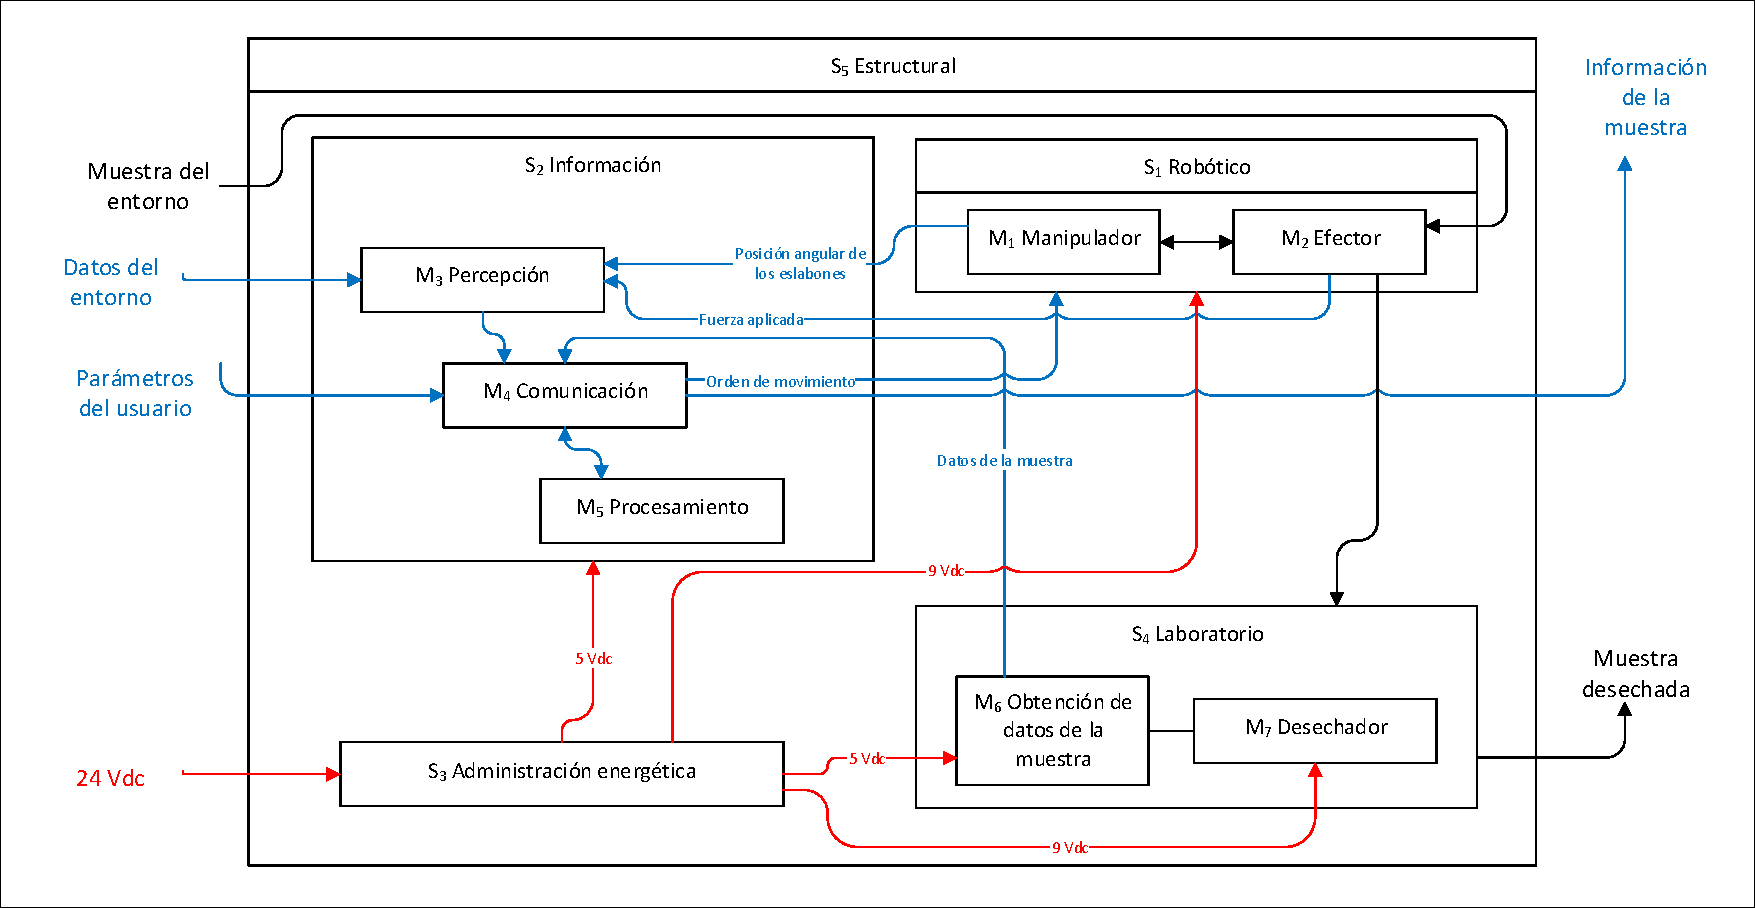
\includegraphics[width=1.5\textwidth ,height=0.8\textheight, trim=4 4 4 4,clip]{imagenes/Modelos/Arquitectura fisica.pdf}
		\caption{Arquitectura f�sica que muestra la interacci�n de los sistemas y m�dulos}
		\label{fig:ArqFis}
	\end{figure}
\end{landscape}


\subsection{Concepto soluci�n}

Una vez que se han determinado los m�dulos que compondr�n el sistema completo, es posible comenzar a proponer soluciones espec�ficas para cada uno, las cuales ser�n sometidas a un proceso de selecci�n utlizando una herramienta de selecci�n multicriterio. 

La Figura \ref{fig:ConceptoS} muestra los modelos tridimensionales de las soluciones propuestas. Estas soluciones comparten diversos aspectos, como son: 1) Una estructura similar a la de un rover, 2) Un brazo de 6 GDL, 3) Bater�a como fuente de alimentaci�n, 4) Sensores de temperatura y 5) C�maras en la parte frontal de la estructura.

El concepto 1 (Figura \ref{fig:ConceptoS}a) tiene un brazo construido de placas paralelas, un gripper con forma de pinza de 2 dedos como efector final, un laboratorio con un cono en la parte superior para guiar la ca�da de la muestra, y circuitos electr�nicos apilados y colocados en el centro de la estructura.

El concepto 2 (Figura \ref{fig:ConceptoS}b) tiene eslabones tubulares, y un efector final similar a los presentes en las excavadoras. Los circuitos tambi�n se encuentran apilados y se ubican en la esquina superior derecha (desde la vista frontal), mientras que el laboratorio est� en la esquina superior izquierda.

El concepto 3 (Figura \ref{fig:ConceptoS}c) cambia en el laboratorio, el cual es un tubo que desliza la muestra hacia la zona de an�lisis y despu�s a un agujero que la deja caer. El efector final es un gripper de 3 dedos.

El concepto 4 (Figura \ref{fig:ConceptoS}d) ubica el laboratorio en el centro del lado izquiedo de la estructura. Los circuitos est�n ubicados lado a lado. El brazo se conforma de eslabones de placas paralelas ranuradas y los actuadores se colocan en una sola base ubicada en la parte frontal.

El concepto 5 (Figura \ref{fig:ConceptoS}e) contiene los mismos elementos que el concepto 1 a excepci�n del efector final, adem�s de que cambian las ubicaciones de los mismos.

El concepto 6 (Figura \ref{fig:ConceptoS}f) contempla los eslabones ranurados y la base se ubica en una esquina, adem�s el laboratorio est� conformado por una placa que tiene la zona de an�lisis, la cual se inclina para que la muestra se deslice hacia un agujero que la deja caer.


% \textbf{Nota: } Los modelos mostrados en la Figura \ref{fig:Concepto1}, \ref{fig:Concepto3}, \ref{fig:Concepto4}, \ref{fig:Concepto5} y \ref{fig:Concepto6} contemplan un recubrimiento protector a los componentes internos (tales como actuadores y transmisiones, entre otros), con el fin de que los a�sle de las condiciones hostiles del ambiente, sin reducir su movilidad.

\begin{figure}
	\centering
	\begin{tabular}{cc}
		\subf{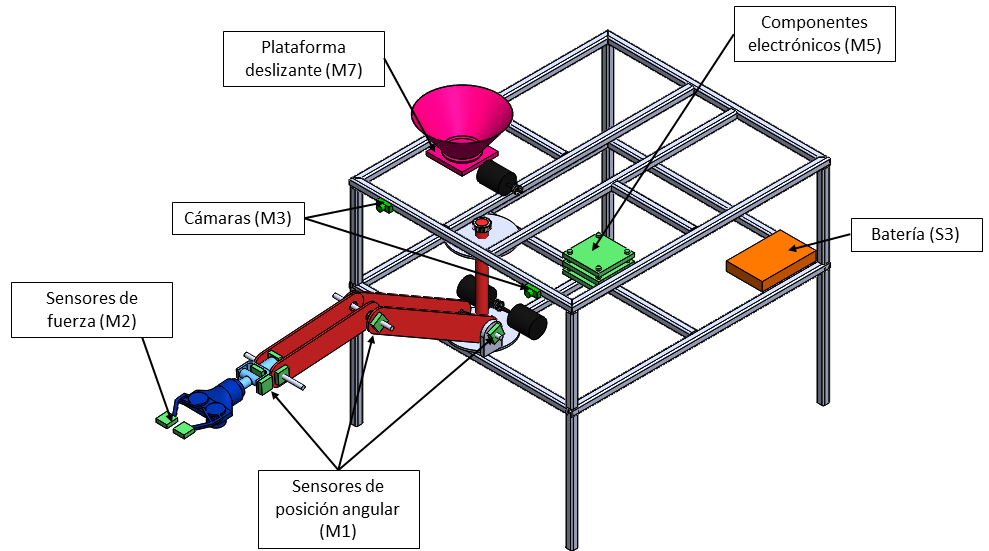
\includegraphics[width=0.45\textwidth, keepaspectratio]{imagenes/Conceptos/Concepto 1 con etiquetas.png}}
			{a}
		&
		\subf{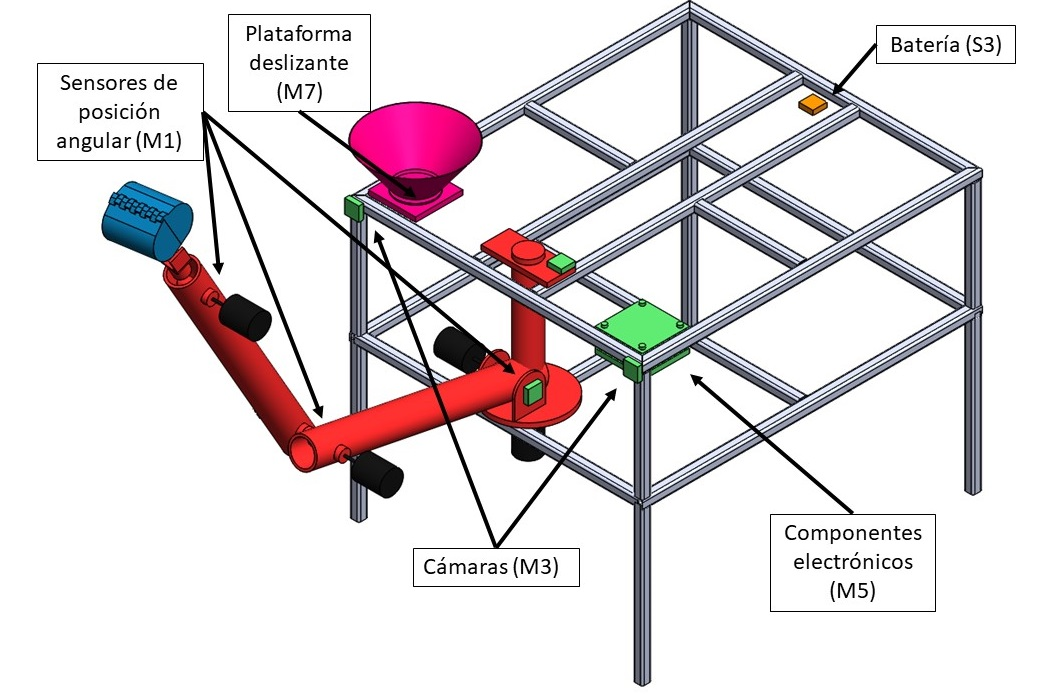
\includegraphics[width=0.4\textwidth, keepaspectratio]{imagenes/Conceptos/Concepto 2 con etiquetas.jpg}}
			{b}
		\\
		\subf{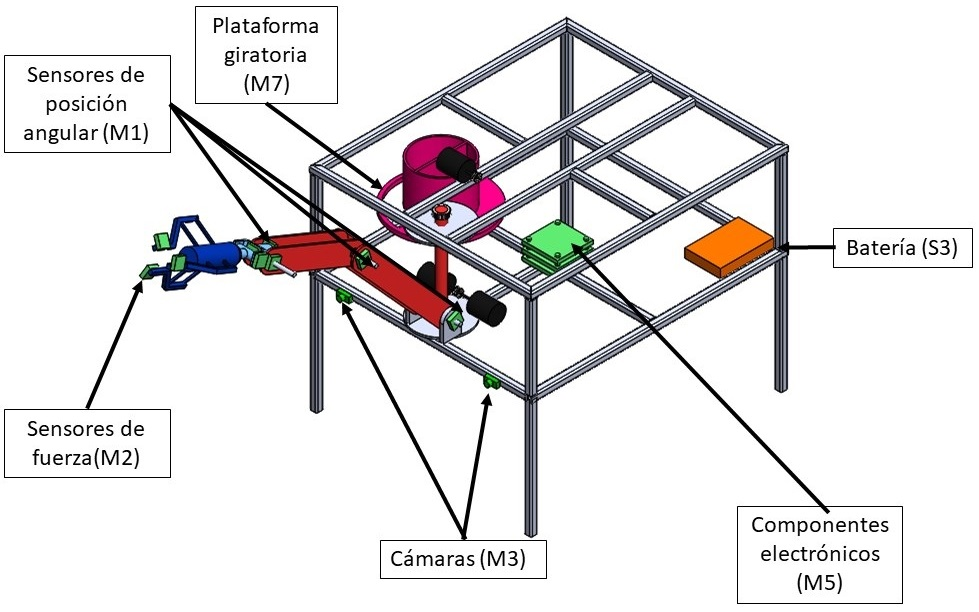
\includegraphics[width=0.45\textwidth, keepaspectratio]{imagenes/Conceptos/Concepto 3 con etiquetas.jpg}}
			{c}
		&
		\subf{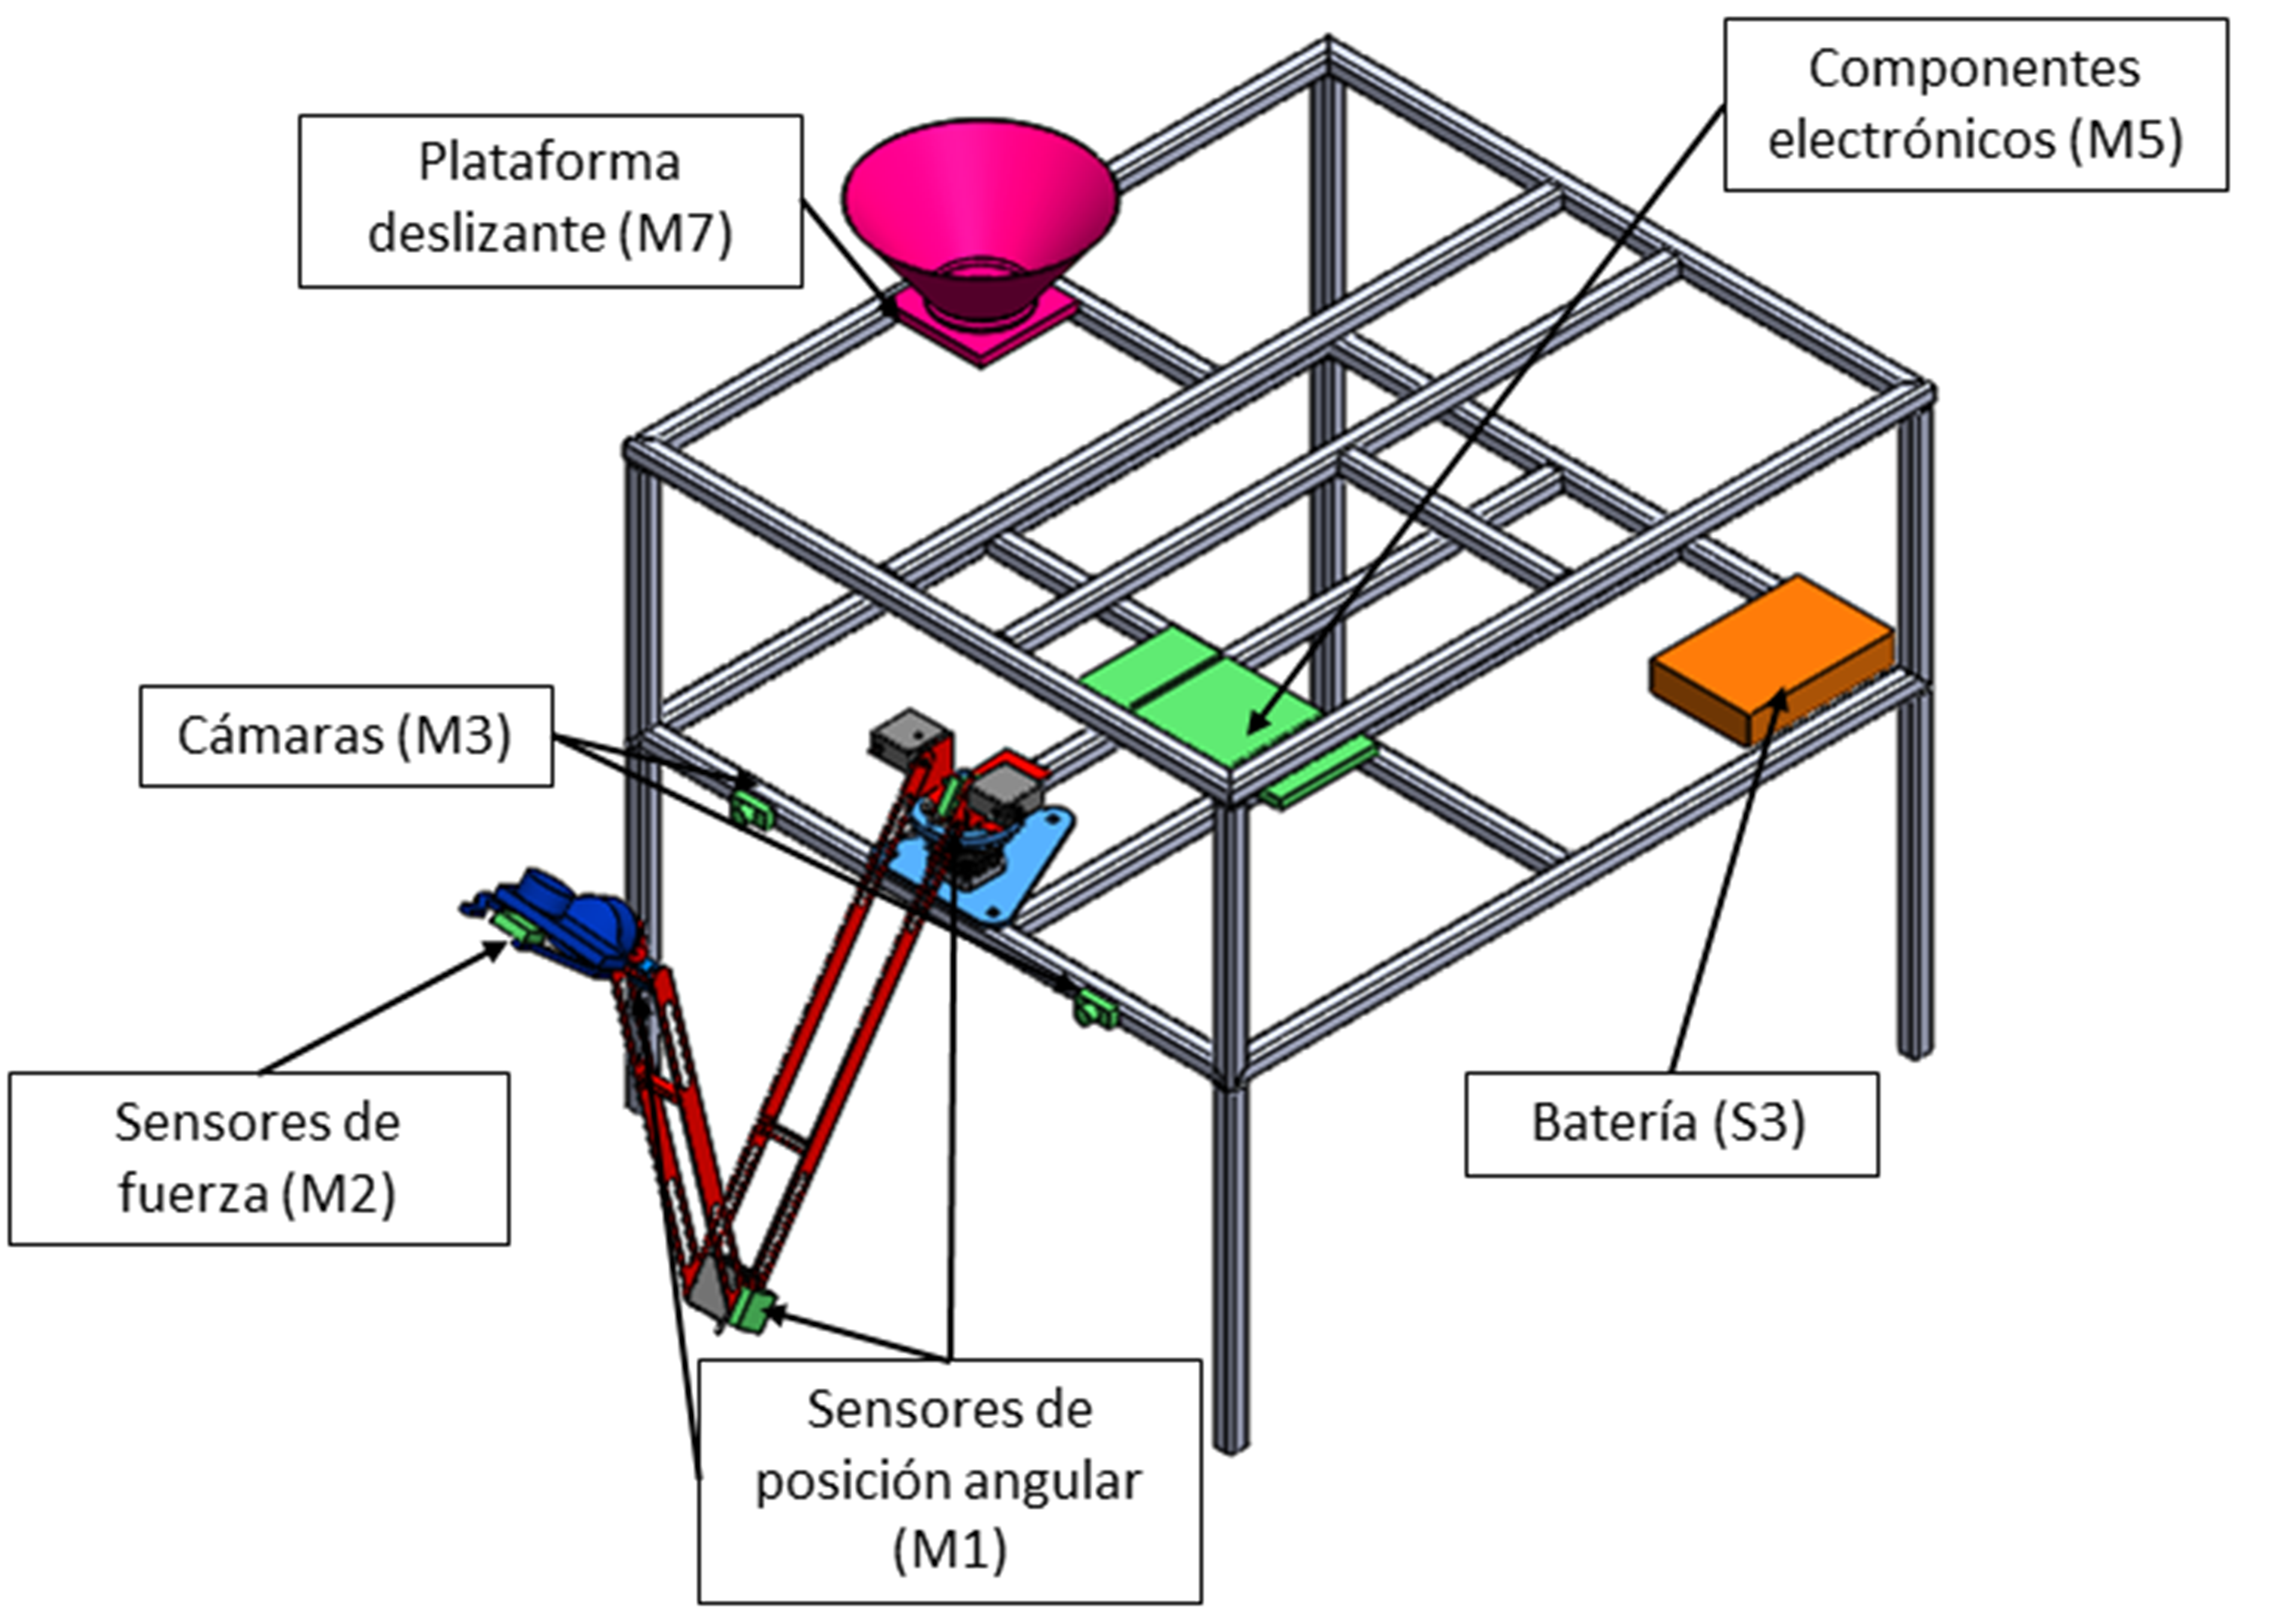
\includegraphics[width=0.45\textwidth, keepaspectratio]{imagenes/Conceptos/Concepto 4 con etiquetas.png}}
			{d}
		\\
		\subf{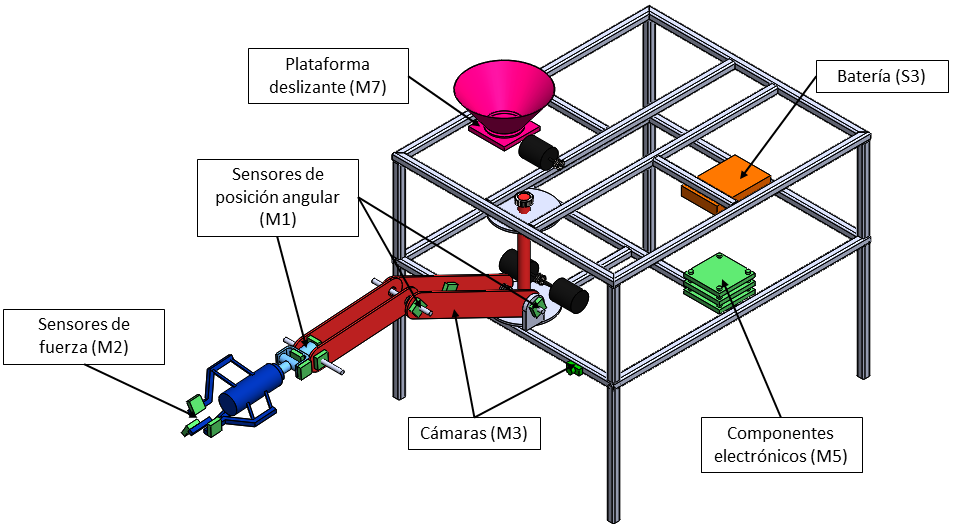
\includegraphics[width=0.45\textwidth, keepaspectratio]{imagenes/Conceptos/Concepto 5 con etiquetas.png}}
			{e}
		&
		\subf{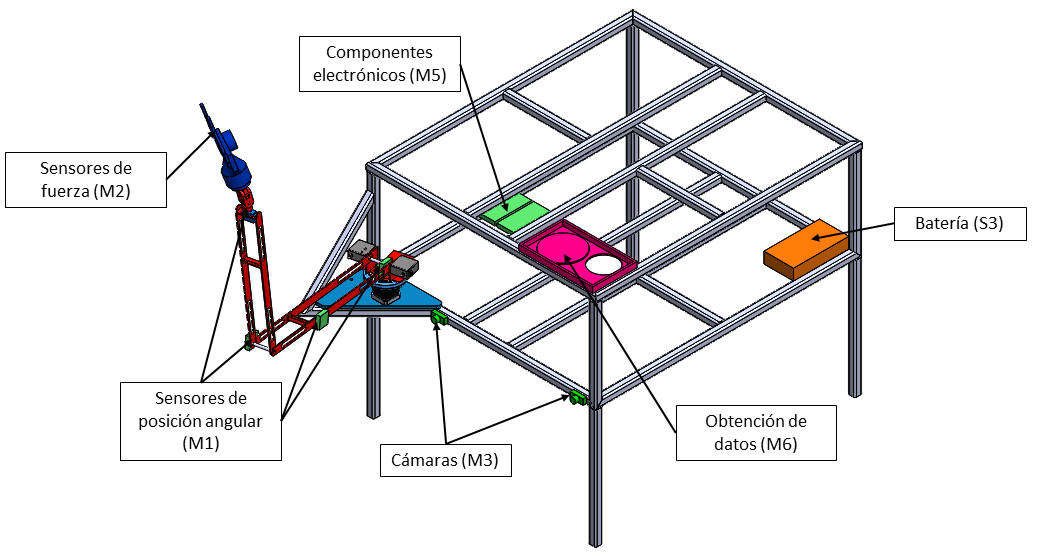
\includegraphics[width=0.45\textwidth, keepaspectratio]{imagenes/Conceptos/Concepto 6 con etiquetas.png}}
			{f}
		\\
	\end{tabular}
	\caption{Conceptos soluci�n}
	\label{fig:ConceptoS}
\end{figure}

Con el objetivo de determinar cu�l es la propuesta que mejor se desempe�a en la realizaci�n de las funciones, se utiliza una herramienta de selecci�n multicriterio denominada \textit{Proceso anal�tico de jerarqu�a}, (\textit{Analytic Hierarchy Process} - AHP por sus siglas en ingl�s)\cite{AHP}; la cual se ayuda de criterios originados a partir del an�lisis de las diferencias que hay entre ellas, los cuales se muestran en el Ap�ndice \ref{Ap:AHP}.

El proceso de selecci�n comienza con una tabla en la que se compara la importancia de cada criterio contra el resto en una relaci�n de 1:1, obteniendo el llamado ``vector de prioridad'', en el cu�l se establece la jerarqu�a de los criterios, como se muestra en el gr�fico de la Figura \ref{fig:AHPJerDes}a, en la cual se puede apreciar que el criterio 13 (Riesgo de da�os a la muestra) es el m�s importante, seguido por el criterio 4 (Riesgo de da�os a la estructura).

Para determinar cual es el concepto que mejor satisface las necesidades, se compara uno a uno el nivel en el que se desmpe�a en cada criterio.

De esta manera, para cada criterio se obtiene un concepto que destaca, y posteriormente se relaciona el desempe�o en cada criterio con la importancia de este, encontrando el valor de desempe�o general de cada concepto, como muestra la Figura \ref{fig:AHPJerDes}b, donde se observa que el mayor valor pertenece al concepto n�mero 5, presentado en la Figura \ref{fig:ConceptoS}e.

\begin{figure}
	\centering
	\begin{tabular}{cc}
		\subf{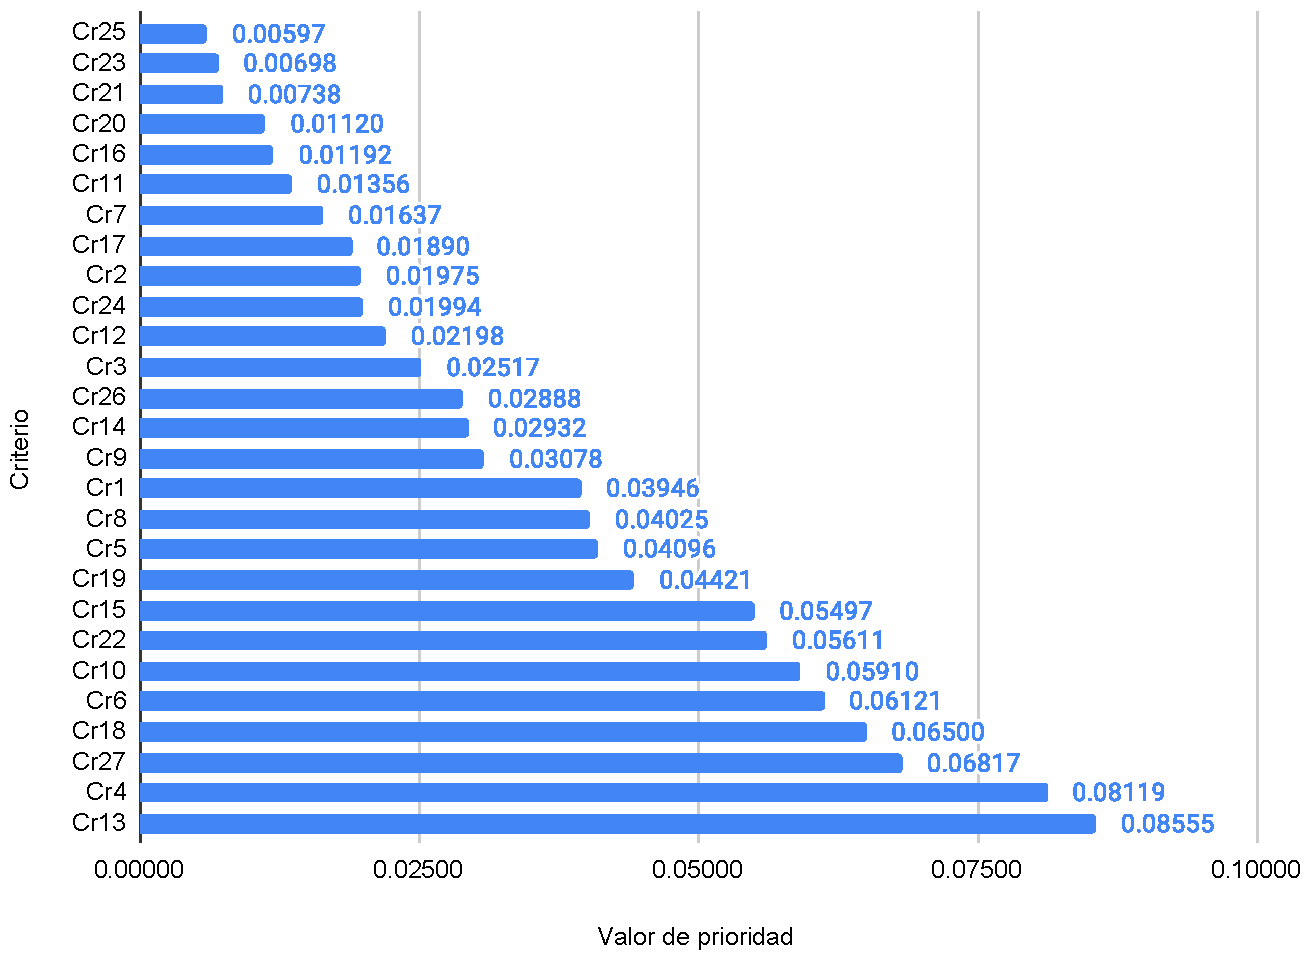
\includegraphics[width=0.45\textwidth, keepaspectratio]{imagenes/Seleccion de concepto/VPCriterios.pdf}}
			{a}
		&
		\subf{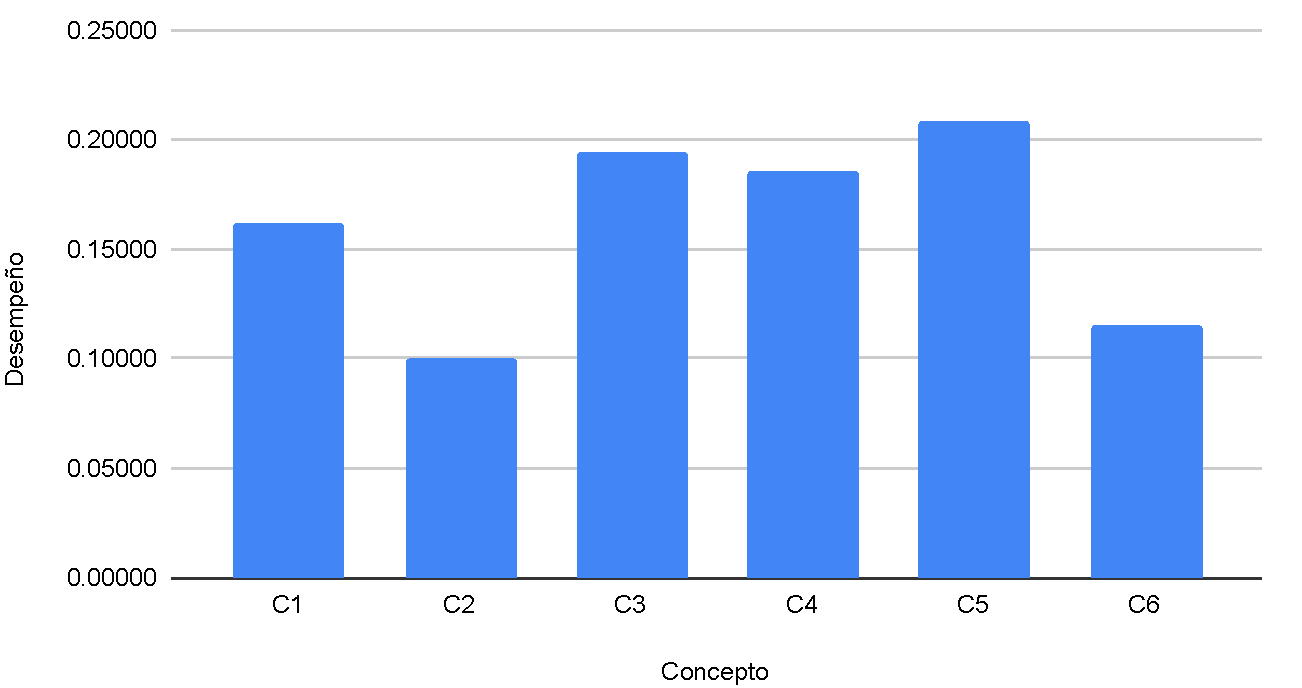
\includegraphics[width=0.45\textwidth, keepaspectratio]{imagenes/Seleccion de concepto/Ganador.pdf}}
			{b}
		\\
	\end{tabular}
	\caption{AHP a) Jerarqu�a de criterios; b) Desempe�o general de los conceptos }
	\label{fig:AHPJerDes}
\end{figure}

El proceso completo se encuentra en el Ap�ndice \ref{Ap:AHP}.

\subsection{Concepto Final}

A pesar de que el concepto n�mero 5 es el concepto elegido (\textbf{Ce}), se puede proponer una nueva configuraci�n, donde se revisa el desempe�o de cada concepto con respecto a los criterios, analiz�ndolos para extraer las caracter�sticas que lo hicieron superior en ese criterio en espec�fico.

Una vez que se han identificado las caracter�sticas a mejorar del \textbf{Ce}, se pueden realizar modificaciones a estas, sin embargo, hay algunas caracter�sticas que est�n contrapuestas. Para determinar el cambio a realizar, se utiliza la Tabla \ref{Tab:ConflictosMejoramiento}, en la cual se comparan las caracter�sticas con sus criterios asociados y sus valores, realizando una suma directa de estos para elegir el que tenga un resultado mayor.

\begin{table}
\centering
\caption{Tabla de comparaci�n de caracater�sticas contrarias para el mejoramiento del concepto elegido}
\begin{scriptsize}
\begin{tabular}{|cccc|}
\hline
\multicolumn{1}{|c|}{Caracter�stica}          	& \multicolumn{1}{c|}{Criterios favorecidos} & \multicolumn{1}{c|}{Valor de los cirterios} & Suma  \\ \hline
\multicolumn{1}{|c|}{Motor acoplado directamente} & \multicolumn{1}{c|}{Cr2}               	& \multicolumn{1}{c|}{0.019}              	& 0.019 \\ \hline
\multicolumn{1}{|c|}{Transmisi�n mec�nica}    	& \multicolumn{1}{c|}{Cr1,Cr4,Cr6}       	& \multicolumn{1}{c|}{0.039,0.081,0.061}  	& 0.181 \\ \hline
                                              	&                                        	&                                         	&   	\\ \hline
\multicolumn{1}{|c|}{Brazo en el centro}      	& \multicolumn{1}{c|}{Cr3,Cr5,Cr6}       	& \multicolumn{1}{c|}{0.025,0.04,0.061}   	& 0.126 \\ \hline
\multicolumn{1}{|c|}{Brazo en un extremo}     	& \multicolumn{1}{c|}{Cr4}               	& \multicolumn{1}{c|}{0.081}              	& 0.081 \\ \hline
                                              	&                                        	&                                         	&   	\\ \hline
\multicolumn{1}{|c|}{Efector de 2 dedos}      	& \multicolumn{1}{c|}{Cr8,Cr11,Cr12}     	& \multicolumn{1}{c|}{0.04,0.013,0.021}   	& 0.074 \\ \hline
\multicolumn{1}{|c|}{Efector de 3 dedos}      	& \multicolumn{1}{c|}{Cr9,Cr10,Cr13}     	& \multicolumn{1}{c|}{0.03,0.059,0.085}   	& 0.174 \\ \hline
\end{tabular}
\end{scriptsize}
\label{Tab:ConflictosMejoramiento}
\end{table}

Por lo tanto, las modificaciones a realizar son: 

\begin{itemize}[noitemsep,nolistsep]
\item Para reducir la potencia, se usa el brazo ranurado con actuadores en la base.
\item Se sustituye el eje largo de acoplamiento a la estructura por una placa similar a la del concepto 4.
\item Se elimina la plataforma deslizable del laboratorio c�nico para recuperar la forma cil�ndrica del concepto 3, lo cual mejora el aprovechamiento del espacio tanto del m�dulo desechador como del de medici�n de peso.
\item Las tarjetas se colocan al centro de la estructura.
\item Se utilizan m�s sensores, ubicados en los componentes de mayor inter�s.
\end{itemize}

\begin{figure}
\centering
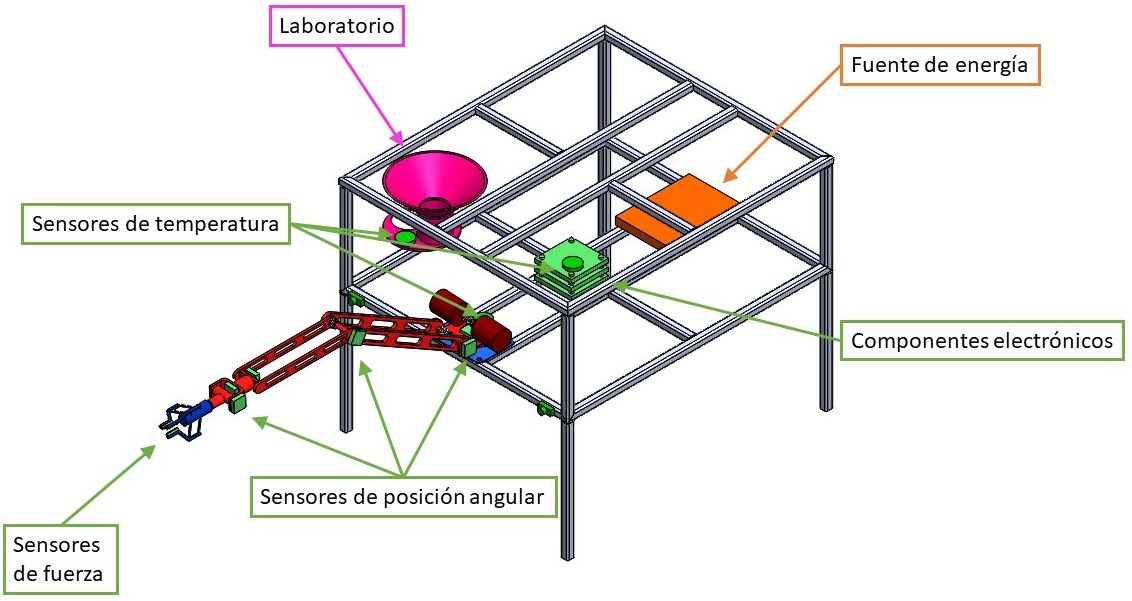
\includegraphics[scale=0.5]{imagenes/Conceptos/Concepto final.jpg}
\caption{Modelo tridimensional del concepto mejorado}
\label{fig:ConceptoMejorado}
\end{figure}

\subsubsection*{Validaci�n de concepto mejorado}

Es necesario someter el \textbf{Cm} a la misma evaluaci�n aplicada a los otros conceptos, comparando �nicamente el \textbf{Ce} con el \textbf{Cm}, de manera que si este �ltimo obtiene un mejor puntaje, significa que las modificaciones realizadas incrementan el desempe�o del sistema.

Tras realizar la evaluaci�n de conceptos, el concepto 5 obtuvo \textit{0.375}, mientras que el \textbf{Cm} obtuvo \textit{0.588}.

La Figura \ref{fig:ConceptoMejorado} muestra el modelo tridimensional del concepto final mejorado (\textbf{Cm}), en el que se han realizado los cambios mencionados previamente.
%%%%%%%%%%%%%%%%%%%%%%%%%%%%%%%%%%%%%%%%%%%%%%%%%%%%%%%%%%%%%%%%%%%
%%%%%%%%%%%%%%%%%%%%%%%%%%%%%%%%%%%%%%%%%%%%%%%%%%%%%%%%%%%%%%%%%%%
\chapter{Dise�o de dominio espec�fico}

A lo largo de este cap�tulo se realiza el dise�o a detalle del sistema, para posteriormente seleccionar los m�todos de manufactura, materiales y componentes f�sicos que conforman los m�dulos pertenecientes al mismo.

\section{Sistema rob�tico (S1)}
\subsection{M�dulo de manipulador (M1)}
\subsubsection*{Brazo antropom�rfico}
Para comenzar el dise�o del manipulador, resulta necesario establecer la distancia horizontal m�xima que debe alcanzar el mismo, la cual se calcula utilizando la ecuaci�n \ref{eq:Pitagorazo}, que corresponde a la ecuaci�n de tri�ngulos rect�ngulos propuesta por Pit�goras, y despejando para obtener el cateto horizontal a partir de la cateto vertical y la hipotenusa mostrados en la figura \ref{fig:AlcancePitagoras}.

\begin{figure}
\centering		
	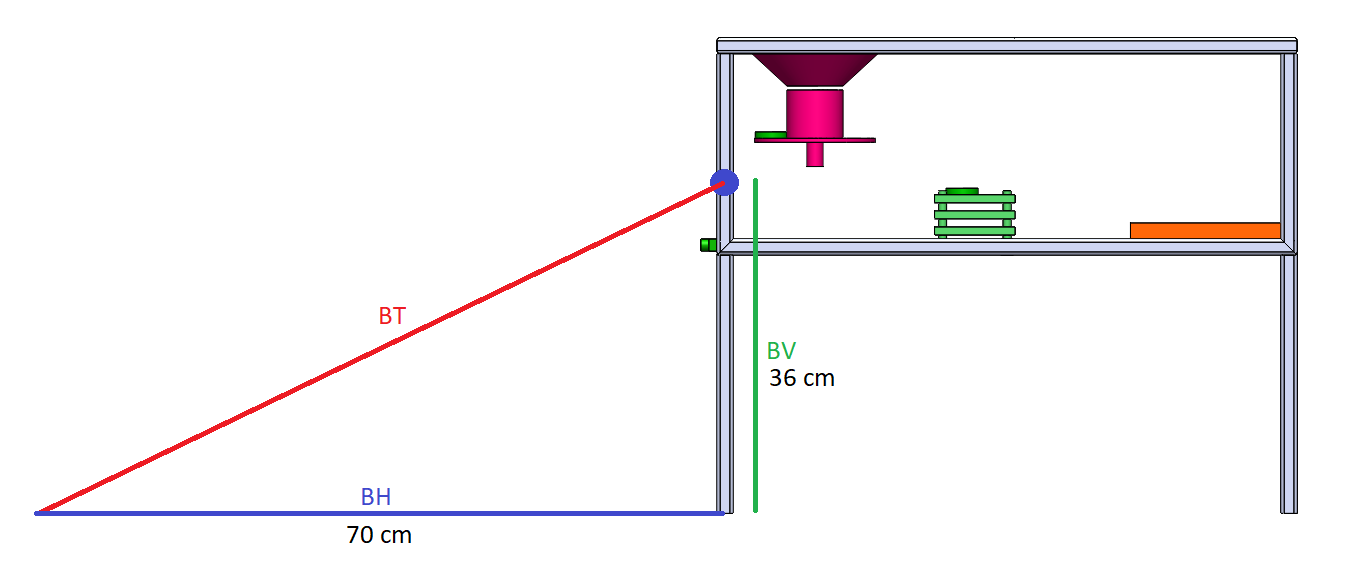
\includegraphics[scale=0.3]{imagenes/Dominio especifico/Vista lateral con brazo}
	\caption{Alcance m�ximo del sistema}
	\label{fig:AlcancePitagoras}
\end{figure}

\begin{equation}
\label{eq:Pitagorazo}
BH = \sqrt{BT^2-BV^2}
\end{equation}
\\ \\
\begin{flushleft}
En donde: $ \; BH =$ Distancia horizontal al punto m�s lejano.
\\
$\qquad \quad \qquad BT =$ Longitud del brazo totalmente estirado.
\\
$\qquad \quad \qquad BV =$ Distancia de la base del robot hasta el suelo.
\end{flushleft}

El objetivo propuesto es que el alcance horizontal del brazo sea de aproximadamente 70cm ($BH 	\approx 70cm$), y tomando en cuenta que la distancia del suelo a la base del robot $BV$ es de 37cm, se requiere una longitud de brazo $BT$ de 79.17 cm, de los cuales 20cm se consideran ocupados por la mu�eca esf�rica y el efector final, quedando 59.17cm libres para los dos eslabones del manipulador.

Adem�s de esto, se establece que la longitud del segundo eslab�n $l_{2}$ sea igual a $3/4$ de la longitud del primero $l_{1}$, resultando en $l_{1}=33.81cm$ y $l_{2}=25.35cm$. Los n�meros enteros m�s cercanos que cumplen esta relaci�n son $l_{1}=32cm$ y $l_{2}=24cm$, los cuales son seleccionados con fines de simplicidad en la manufactura.

De esta manera, las longitudes quedan como se muestra a continuaci�n:

\begin{flushleft}
$\qquad \quad \qquad BT = 76cm$
$\qquad \quad \qquad BH = 66.38cm$
$\qquad \quad \qquad BV = 37cm$
\end{flushleft}

\subsubsection*{Selecci�n de material para eslabones}

Con el fin de determinar el material para construir el sistema rob�tico, se debe considerar su geometr�a, tomando en consideraci�n la restricci�n de masa (R5). Se considera de forma preliminar que la base fija al rover tenga una masa de 2 Kg, lo cual deja 10 Kg disponibles para el manipulador, adem�s de que se determina un factor de seguridad para la masa de la muestra igual a 2, y el efector final tiene una masa de 2Kg\cite{GripperOS}, el cual se discute en la secci�n Efector Final (M2)(Vinculo), quedando 7.5 Kg para el manipulador.

Con el objetivo de generar reacciones peque�as, se establece que el primer eslab�n ocupe la mayor parte de la masa, ya que es el que soporta al resto del manipulador, mientras que el eslab�n 2 y la mu�eca deben ser m�s ligeros que el primer eslab�n al estar m�s lejos de los ejes de giro de los primeros 2 GDL, por lo que se reduce la masa asignada en un Kg para cada elemento, quedando de la siguiente manera:

\begin{itemize}[noitemsep,nolistsep]
\item Eslab�n 1: \unit[3.5]{Kg}.
\item Eslab�n 2: 2.5 Kg.
\item Mu�eca: 1.5 Kg.
\item Efector final: 2 Kg.
\item Muestra: 500 g.
\end{itemize}

Contando con estos datos, es posible calcular la densidad m�xima que debe poseer el material a utilizar, consultando el gr�fico que relaciona la densidad de los materiales con su respectivo m�dulo de elasticidad propuesto por Michael Ashby\cite{Ashby}, el cual puede ser observado en la Figura \ref{fig:DensidadVSYoung}.

\subsubsection*{Dise�o de geometr�a de los eslabones}

La geometr�a del primer eslab�n est� determinada por las siguientes dimensiones:

\begin{itemize}[noitemsep,nolistsep]
\item Longitud: 32 cm.
\item Espesor: 8 mm.
\item Alto: 3 cm.
\item Radio de chafl�n: 1.5 cm.
\end{itemize}

Con estos datos es posible calcular el volumen ocupado por el mismo, separ�ndolo en sus geometr�as b�sicas, que son un cilindro y un prisma rectangular, adem�s de considerar el volumen de los ejes utilizados para unir ambos perfiles de cada eslab�n, por lo que se debe sumar el volumen de �stos, y restar el volumen del barreno requerido para acoplarlos, sustituyendo las dimensiones en la ecuaci�n \ref{eq:VolumenE1} 

\begin{equation}
\label{eq:VolumenE1}
V_{e} = 2t_{e}(h_{e}l_{e} + \pi r^2_{e}-50 \pi)+400 \pi  
\end{equation}

\begin{flushleft}
En donde: $ \; V_{e} =$ Volumen ocupado por el eslab�n.
\\
$\qquad \quad \qquad t_{e} =$ Espesor del perfil del eslab�n.
\\
$\qquad \quad \qquad h_{e} =$ Altura del perfil del eslab�n.
\\
$\qquad \quad \qquad l_{e} =$ Longitud del perfil del eslab�n.
\\
$\qquad \quad \qquad r_{e} =$ Radio del chafl�n del eslab�n.
\end{flushleft}

Sustituyendo $t_{e_{1}}$,$h_{e_{1}}$,$l_{1}$ y $r_{e_{1}}$ en la ecuaci�n \ref{eq:VolumenE1}, queda lo siguiente:


\begin{center}
$V_{e_{1}} = \unit[174.962e-6]{m^3}$
\end{center}


Una vez que se ha calculado el volumen que ocupa el eslab�n con las dimensiones especificadas, y utilizando el valor de su masa determinada, es posible calcular la densidad m�xima que debe tener el material, cuyo valor est� dado por la ecuaci�n \ref{eq:DensidadE1}, recordando que el concepto soluci�n contempla dos placas paralelas, por lo que el peso determinado debe distribuirse equitativamente.

\begin{equation}
\label{eq:DensidadE1}
\rho_{e} = \frac{m_{e}}{2V_{e}}
\end{equation}

\begin{flushleft}
En donde: $ \; m_{e} =$ Masa del eslab�n.
\\
$\qquad \quad \qquad \rho_{e} \: \; =$ Densidad del eslab�n.
\end{flushleft}


Sustituyendo $m_{e_{1}}$ y $V_{e_{1}}$ en la ecuaci�n \ref{eq:DensidadE1}, queda lo siguiente:

\begin{center}
 $\rho_{e_{1}} = \unitfrac[10002.17]{Kg}{m^3}$ 
 \end{center} 
 
Una vez que se conoce la densidad m�xima $\rho_{e_{1}}$ del material a seleccionar, se analiza la relaci�n entre la densidad y el m�dulo de elasticidad de los materiales mostrada en el gr�fico de la Figura \ref{fig:DensidadVSYoung_Seleccion}, que indica aquellos materiales que no se pueden elegir con un �rea sombreada, debido a que su densidad es mayor a la m�xima establecida en el c�lculo anterior, mostrando que la variedad de materiales entre los que se puede elegir es amplia. Esto incluye a los metales, los cuales son una buena elecci�n debido a su m�dulo de elasticidad elevado, sobresaliendo entre �stos el aluminio, muy utilizado en aplicaciones aeroespaciales debido a su alta maquinabilidad sin comprometer el peso. En la Tabla \ref{tab:PropiedadesAluminio} se muestran las principales propiedades mec�nicas del mismo\cite{SolidWorks}.

\begin{figure}
\centering		
	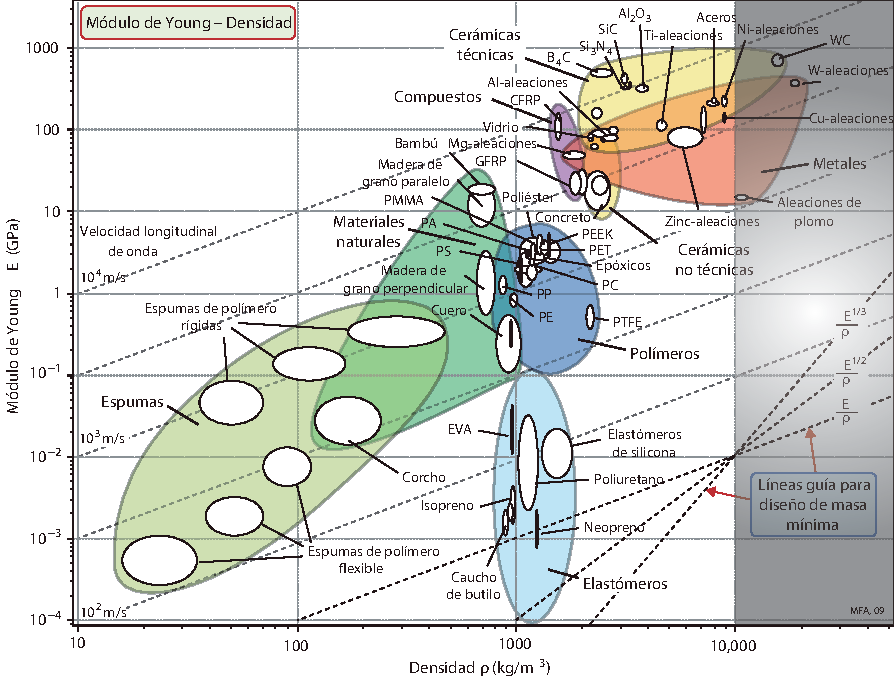
\includegraphics[scale=1]{imagenes/Dominio especifico/DensidadVSYoung_Seleccion}
	\caption{Rango de materiales elegibles para el eslab�n}
	\label{fig:DensidadVSYoung_Seleccion}
\end{figure}

\begin{table}
\caption{Propiedades mec�nicas del Aluminio 6061 T6}
\centering
\begin{scriptsize}
\begin{tabular}{|c|c|c|}
\hline
Propiedad              & Valor & Unidades \\ \hline
Densidad               & 2700  & $\unitfrac{Kg}{m^3} $   \\ \hline
M�dulo el�stico        & 69    & GPa      \\ \hline
Coeficiente de Poisson & 0.33  & adimensional         \\ \hline
\end{tabular}
\end{scriptsize}
\label{tab:PropiedadesAluminio}
\end{table}

Para seleccionar el material del segundo eslab�n se sigue el mismo procedimiento, utilizando las dimensiones determinadas, las cuales son:

\begin{itemize}[noitemsep,nolistsep]
\item Longitud: 24 cm.
\item Espesor: 6 mm.
\item Alto: 2.25 cm.
\item Radio de chafl�n: 1.125 cm.
\end{itemize}

Con estos datos se calcula el volumen y la densidad sustituy�ndolos en las ecuaciones \ref{eq:VolumenE1} y \ref{eq:DensidadE1} como sigue:

\begin{center}
$V_{e_{2}}   = \unit[80.252e-6]{m^3}$
\\
$\rho_{e_{2}} = \unitfrac[15575.93]{Kg}{m^3}$
\end{center}

Como en el caso anterior, el c�lculo demuestra que hay muchos materiales entre los cuales elegir, por lo que se selecciona nuevamente el aluminio, ya que presenta la ventaja a�adida de que es m�s barato comprar el mismo material en mayor cantidad que una cantidad menor de distintos materiales.

Considerando que unos eslabones s�lidos tienen factores de seguridad grandes, y dado que uno de los objetivos del proyecto es reducir el consumo energ�tico del sistema, se realizaron varios redise�os en las cuales se reduce la cantidad de material ranurando los eslabones y modificando la secci�n transversal, resultando en las siguientes dimensiones:

\begin{itemize}[noitemsep,nolistsep]
\item $t_{e{1}} =$ 6.35 mm
\item $t_{e{2}} =$ 6 mm
\end{itemize}

Los eslabones redise�ados pueden observarse en las Figuras \ref{fig:CADE1Ran} y \ref{fig:CADE2Ran}.

\begin{figure}
	\centering		
		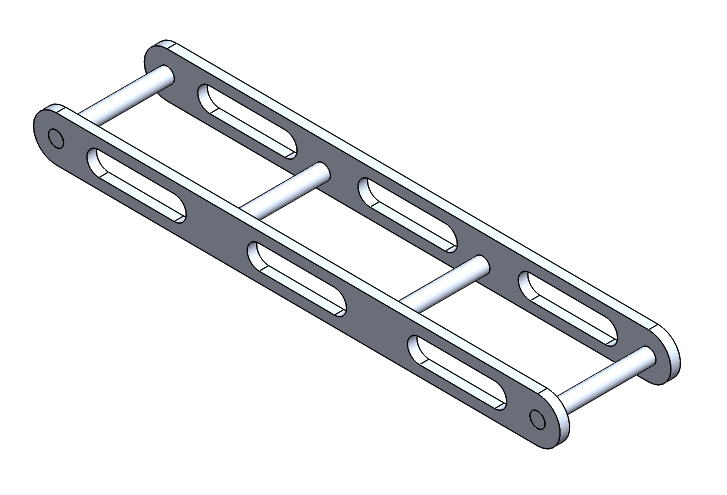
\includegraphics[scale=0.5]{imagenes/Dominio especifico/Validaciones eslabones/Primeros eslabones ranurados}
		\caption{Modelo CAD del primer eslab�n ranurado.}
		\label{fig:CADE1Ran}
\end{figure}

\begin{figure}
	\centering		
		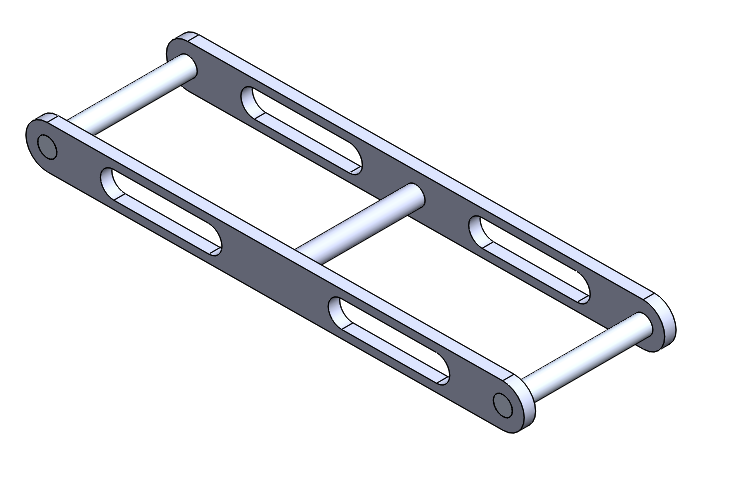
\includegraphics[scale=0.5]{imagenes/Dominio especifico/Validaciones eslabones/Segundos eslabones ranurados}
		\caption{Modelo CAD del segundo eslab�n ranurado.}
		\label{fig:CADE2Ran}
\end{figure}

El volumen ocupado por los eslabones y la masa de los mismos son los siguientes:

\begin{itemize}[noitemsep,nolistsep]
	\item $V_{e{1}} =113.899e-6 m^{3}$
	\item $V_{e{2}} =65.098e-6 m^{3}$
	\item $m_{e{1}} =307.53g$ 
	\item $m_{e{2}} =175.77g$ 
\end{itemize}

\subsubsection*{Validaci�n de la selecci�n}

Para comprobar el rendimiento del material frente a las cargas aplicadas se ejecuta un an�lisis de elemento finito est�tico\cite{FEASolid} realizando un estudio de resistencia a cada elemento en el software SolidWorks 2018\textregistered \cite{SolidWorks}.

Para poder ejecutar este an�lisis, el software requiere que el usuario indique el valor de las cargas a las que el elemento est� sometido, por lo tanto, se calculan las cargas equivalentes mediante las ecuaciones est�ticas de equilibrio, siendo la ecuaci�n \ref{eq:SumaFuerzas} la correspondiente a la suma de fuerzas y la ecuaci�n \ref{eq:SumaMomentos} a la suma de momentos.

\begin{equation}
\label{eq:SumaFuerzas}
\uparrow \sum F_{y} = 0 
\end{equation}

\begin{flushleft}
En donde: $ \; F_{y} =$ Fuerzas existentes en el eje Y.
\end{flushleft}

\begin{equation}
\label{eq:SumaMomentos}
\circlearrowleft \sum M_{o} = 0
\end{equation}

\begin{flushleft}
En donde: $ \; M_{o} =$ Momentos generados por las fuerzas normales al punto O.
\end{flushleft}



\begin{figure}
\centering		
	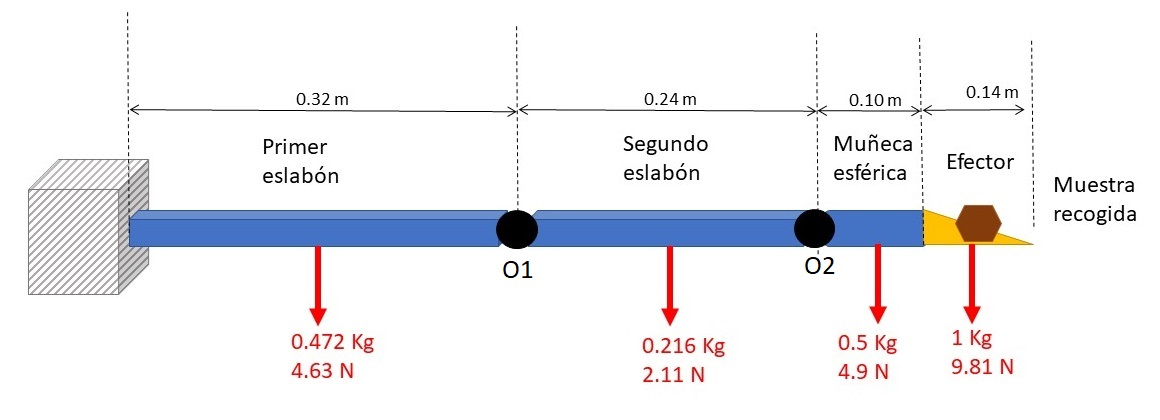
\includegraphics[scale=0.5]{imagenes/Dominio especifico/Validaciones eslabones/DP1}
	\caption{Cargas aplicadas al sistema con eslabones ranurados}
	\label{fig:CargasSRan}
\end{figure}

En la Figura \ref{fig:CargasSRan} se pueden apreciar las cargas a las que est� sometido el sistema, analizando las cargas aplicadas en el eslab�n 1 en la Figura \ref{fig:CargasE1Ran}, mientras que las cargas aplicadas al eslab�n 2 son mostradas en la Figura \ref{fig:CargasE2Ran}. Estos datos proporcionan la informaci�n necesaria para hacer las simulaciones.

\begin{figure}
\centering		
	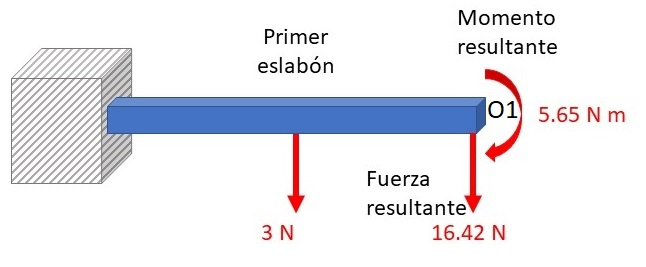
\includegraphics[scale=0.5]{imagenes/Dominio especifico/Validaciones eslabones/E12}
	\caption{Cargas aplicadas al eslab�n 1 ranurado.}
	\label{fig:CargasE1Ran}
\end{figure}

\begin{figure}
\centering		
	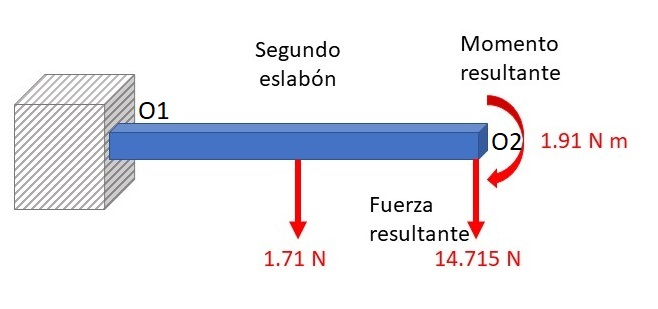
\includegraphics[scale=0.5]{imagenes/Dominio especifico/Validaciones eslabones/E22}
	\caption{Cargas aplicadas al eslab�n 2 ranurado.}
	\label{fig:CargasE2Ran}
\end{figure}

Los estudios de los eslabones se muestran en las Figuras \ref{fig:AnE1Ran} y \ref{fig:AnE2Ran} respectivamente, mostrando en color rojo las �reas en las que el esfuerzo von Mises es mayor, reduciendo la magnitud as� como cambiando el color a azul en las �reas en las que es menor.

\begin{figure}
\centering		
	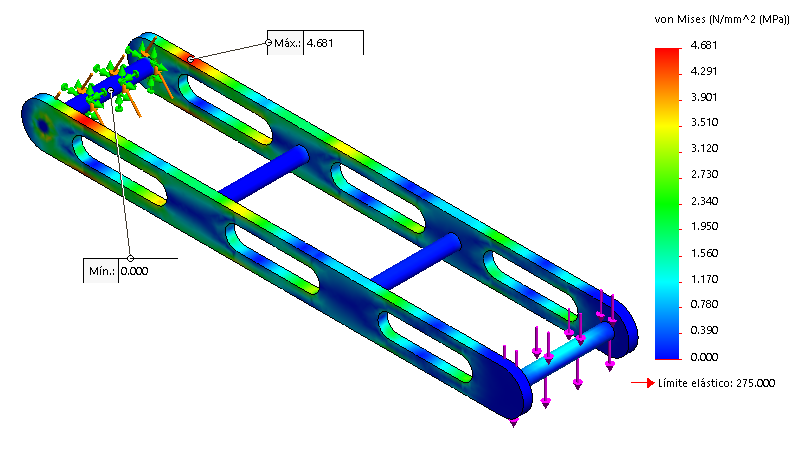
\includegraphics[scale=0.5]{imagenes/Dominio especifico/Validaciones eslabones/Eslabon_1_ranurado}
	\caption{Estudio de resistencia del eslab�n 1 ranurado}
	\label{fig:AnE1Ran}
\end{figure}

\begin{figure}
\centering		
	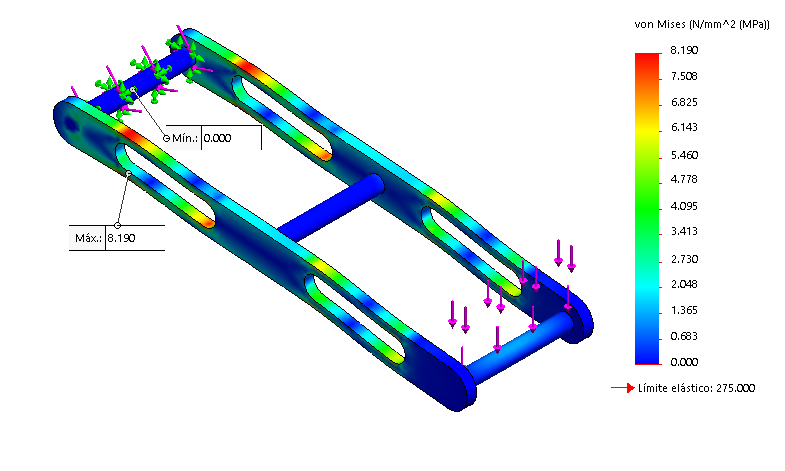
\includegraphics[scale=0.5]{imagenes/Dominio especifico/Validaciones eslabones/Eslabon_2_ranurado}
	\caption{Estudio de resistencia del eslab�n 2 ranurado}
	\label{fig:AnE2Ran}
\end{figure}

El esfuerzo von Mises m�ximo de 4.681 MPa en el primer eslab�n y 8.19 MPa en el segundo arrojan un factor de seguridad de 58.74 y 33.57 respectivamente, por lo que es posible concluir que se logr� reducir la masa en un 30\% en comparaci�n a eslabones s�lidos sin que el material falle.

\subsubsection*{Selecci�n de actuadores para los eslabones}

Para seleccionar los motores, es necesario determinar el torque que el motor debe aplicar para poder mover al sistema y la muestra, indicada en la Figura \ref{fig:CarMot1} para el segundo GDL, y la Figura \ref{fig:CarMot2} para el tercer GDL.

\begin{figure}
\centering		
	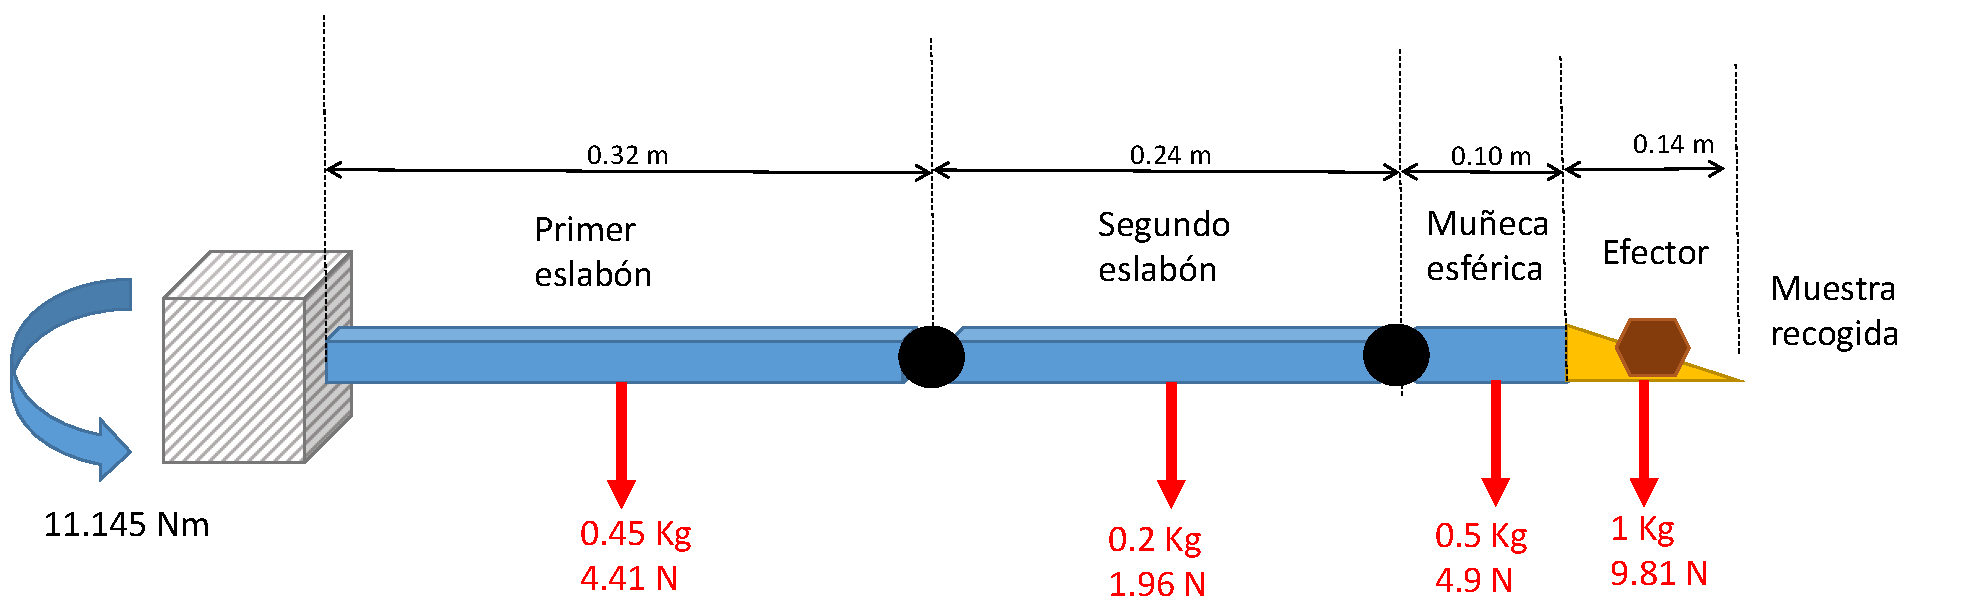
\includegraphics[scale=0.5]{imagenes/Dominio especifico/Validaciones eslabones/TorMot1}
	\caption{Diagrama de cargas aplicadas al motor del primer eslab�n}
	\label{fig:CarMot1}
\end{figure}

\begin{figure}
\centering		
	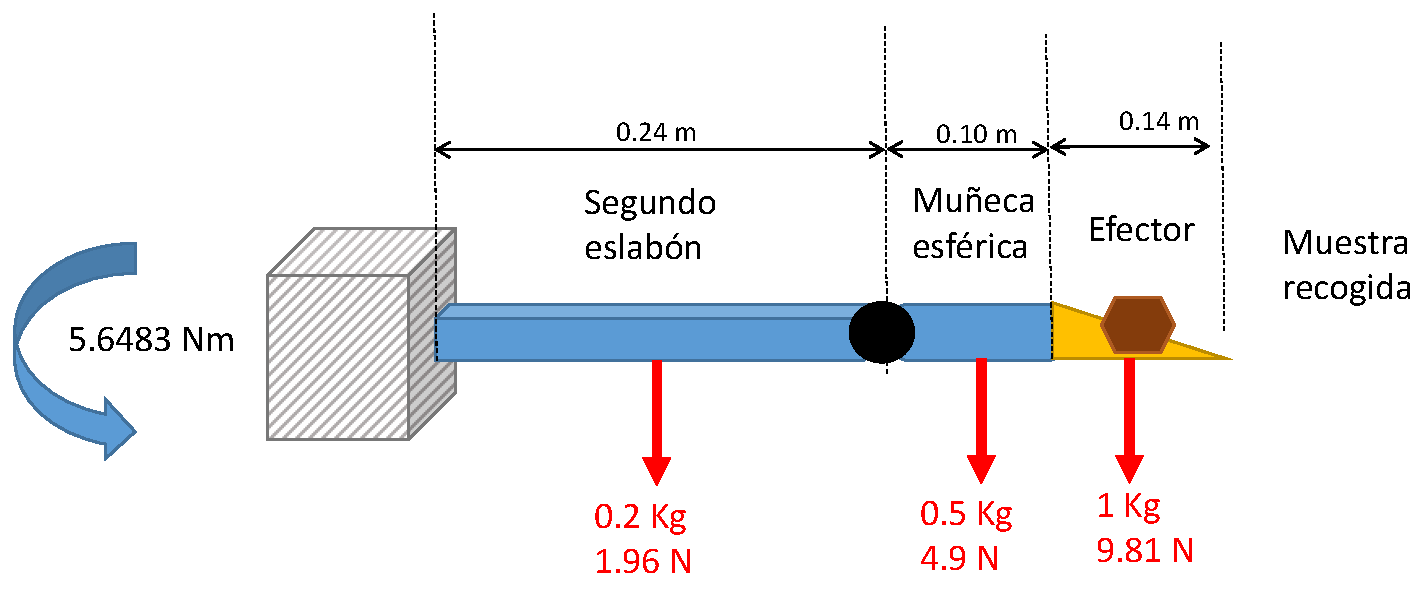
\includegraphics[scale=0.5]{imagenes/Dominio especifico/Validaciones eslabones/TorMot2}
	\caption{Diagrama de cargas aplicadas al motor del segundo eslab�n}
	\label{fig:CarMot2}
\end{figure}

Conociendo este valor, se comparan diversos motores en el mercado utilizando el �rbol de decisiones mostrado en el Ap�ndice \ref{ApA1:MotCD}, y se selecciona el motorreductor Planetario Premium HD 12V, 23RPM 4166.2oz-in con codificador, fabricado por Servo City, que de acuerdo a la hoja de especificaciones (Anexo \ref{An:Mot}), cuenta con las siguientes caracter�sticas.

\begin{itemize}[noitemsep,nolistsep]
\item Par m�ximo = 4166.2 oz-in = 29.4198 Nm
\item Velocidad nominal = 23 rpm
\item Corriente sin carga = 0.54 A
\item Corriente de motor bloqueado = 20[A]
\item Voltaje de alimentaci�n = 12 V
\item Relaci�n de transmisi�n = 369:1
\end{itemize}

Conociendo la corriente del motor bloqueado, y el par m�ximo se calcula la constante de par $K_{m}$ de acuerdo a la ecuaci�n \ref{eq:KmMotor}.

\begin{align*}
K_{m} = \frac{29.5[N-m]}{20[A]}=1.475\unitfrac{N-m}{A}
\end{align*}

\textbf{Validaci�n de actuadores}

Para comprobar que los motores seleccionados son capaces de mover la carga determinada, se calcula el factor de seguridad.

\textit{Par necesario para el segundo GDL = 11.145 Nm ; FS = 2.639}\\
\textit{Par necesario para el tercer GDL = 5.6483 Nm ; FS = 5.208}

Con estos pares calculados, y dspejando para $i_{a}$ de la ecuaci�n \ref{eq:KmMotor}, se puede calcular la corriente esperada.

\begin{align}
i_{a} = \frac{\tau_{0}}{K_{m}}=\frac{11.145N-m}{1.475\unitfrac{N-m}{A}} = 7.55[A]
\end{align}

\subsubsection*{Transmisi�n mec�nica}

Las bandas s�ncronas son cada vez m�s utilizadas en aplicaciones donde antes se consideraba utilizar engranes o cadenas\cite{Mott}, pues tienen la ventaja de presentar bajas vibraciones de operaci�n, poco ruido, facilidad de determinar la posici�n actual entre otras, sin sacrificar la capacidad de carga que pueden mover. Por esta raz�n, se utilizan bandas para transmitir la potencia generada por los actuadores.
Los par�metros que debe cumplir la banda de transmisi�n son los siguientes:

\begin{itemize}[noitemsep,nolistsep]
\item Velocidad de movimiento del efector: $0.05 \unitfrac{m}{s}$
\item Relacion de velocidad: \textit{1:1}
\end{itemize}

Para calcular la potencia que debe transmitir la banda de cada eslab�n (ecuaci�n \ref{eq:PotBanda}), se toman en cuenta los pares necesarios (mostrados en las Figuras \ref{fig:CarMot1} y \ref{fig:CarMot2} respectivamente), y la velocidad angular a la que gira el eje del motor, recordando que es la misma de la banda y utilizando la ecuaci�n \ref{eq:VTang} como sigue.

\begin{align*}
\omega_{1} &= v/r= \frac{.05\unitfrac{m}{s}}{0.73m} = 0.068 \unitfrac{rad}{s} = 0.64 rpm\\
\omega_{2} &= \frac{.05\unitfrac{m}{s}}{0.41m} = 0.121 \unitfrac{rad}{s} = 1.15 rpm\\
P_{1} &= \tau_{1} \omega_{1} = 11.145Nm*0.068\unitfrac{rad}{s} = 0.757 W = 0.0010 HP\\
P_{2} &= \tau_{2} \omega_{2} = 5.6483Nm*0.121\unitfrac{rad}{s} = 0.683 W = 0.0009 HP
\end{align*}

El ajuste de potencia se determina con la ecuaci�n \ref{eq:PotDis}, utilizando un factor de servicio de 1.1, asociado con aplicaciones de carga ligera en periodos de 8 horas diarias (servicio intermitente)\cite{Mott}, y queda como sigue:

\begin{align*}
P_{1-ajustada} &= 0.757W*1.1=0.8327 W = 0.0014 HP\\
P_{2-ajustada} &= 0.683W*1.1=0.7513 W = 0.0012 HP
\end{align*}

Para determinar el paso m�nimo de la transmisi�n se utiliza la tabla del fabricante SDP/SI\cite{BandasSDP}, con el valor de potencia y la velocidad de operaci�n, lo que indica que una banda de perfil XL es adecuada para esta aplicaci�n en ambos eslabones.
La longitud de la banda est� determinada por dos factores, la distancia entre centros y el di�metro de las poleas, por lo que se procede a realizar su selecci�n.

Dado que el di�metro de la polea es directamente proporcional a su n�mero de dientes para mantener el paso, se busca para la polea conducida el n�mero m�nimo est�ndar de dientes para poleas con di�metro interno de 12mm (de acuerdo al dise�o del eje, tratado en la p�gina), el cual es de 15 dientes, por lo que se selecciona la polea A 6A 3-15DF03716 de SDP/SI (Anexo \ref{An:PolSDP}). Por lo tanto, para la polea conductora se requiere una polea de di�metro interno de 6mm (di�metro del eje del motor), con 15 dientes para mantener la relaci�n de velocidad especificada, siendo elegida la polea Actobotics 15D (Anexo \ref{An:Pol15}).

Con el valor del di�metro de la polea, se calcula la longitud de cada banda con la ecuaci�n \ref{eq:LongBanda}.

\begin{align*}
L_{entre \: ejes} &=  2*320[mm]+15*5.080[mm] = 716.2[mm] = 28.19[in] = 145\: ranuras\\
L_{motor \: a \: eje} &=  2*44.6[mm]+15*5.080[mm] = 165.4[mm] = 6.511[in] = 35\: ranuras
\end{align*}

Las bandas XL se encuentran en el mercado con anchos entre 0.25[in] y 0.375[in].
Una vez que se conocen los datos necesarios para las bandas, se seleccionan los modelos de ServoCity B375-290XL con 145  ranuras y B375-70XL  con 35 ranuras.

Conociendo estos datos, se calcula la potencia base nominal ajustada\cite{Mott} utilizando la ecuaci�n \ref{eq:PotBandAjus} como sigue:

\begin{align*}
& P_{1-ajustada} = 0.0014 HP * 1 = 0.0014 HP\\
& P_{2-ajustada} = 0.0012 HP * 0.7 = 0.0008 HP
\end{align*}

Para comprobar que la banda opera con niveles bajos de ruido, se calcula la velocidad lineal de la banda, y para ello se utiliza la ecuaci�n \ref{eq:VelBandRuido}.

\begin{align*}
V_{banda-1}&=\frac{12.7[mm]*0.068\left[\unitfrac{m}{s}\right]}{2}=0.431 m/s\\
V_{banda-2}&=\frac{12.7[mm]*0.121\left[\unitfrac{m}{s}\right]}{2}=0.768 m/s
\end{align*} 

Ya que la velocidad en ambas bandas es menor a 17.78 m/s, que es la velocidad m�xima a la que puede operar la banda sin perturbaciones\cite{Mott}, se comprueba que las bandas no operan con ruido.

Las caracter�sticas de las bandas seleccionadas se muestran en la tabla \ref{tab:BandasModelos}.

\begin{table}
	\centering
	\caption{Caracter�sticas de las bandas seleccionadas}
	\label{tab:BandasModelos}
	\scriptsize
	\begin{tabular}{|c|c|c|} 
	\cline{2-3}
	\multicolumn{1}{c|}{} & Primer eslab�n & Segundo eslab�n      \\ 
	\hline
	Modelo                & B375-70XL      & B375-290XL           \\ 
	\hline
	Paso                  & \multicolumn{2}{c|}{0.200 (XL)}       \\ 
	\hline
	Material              & \multicolumn{2}{c|}{Neopreno}         \\ 
	\hline
	N�mero de ranuras     & 35             & 145                  \\ 
	\hline
	Material tensor       & \multicolumn{2}{c|}{Fibra~de~vidrio}  \\ 
	\hline
	Ancho [in]            & \multicolumn{2}{c|}{3.75}             \\ 
	\hline
	Largo [in]            & 7              & 29                   \\
	\hline
	\end{tabular}
\end{table}

\begin{table}
	\centering
	\caption{Caracter�sticas de las poleas seleccionadas}
	\label{tab:PoleasModelos}
	\scriptsize
	\begin{tabular}{|c|c|c|} 
	\cline{2-3}
	\multicolumn{1}{c|}{}      & Conductora & Conducida                         \\ 
	\hline
	Material                   & \multicolumn{2}{c|}{Aluminio 6061 T6}          \\ 
	\hline
	Ancho m�ximo de banda [in] & \multicolumn{2}{c|}{0.375}                     \\ 
	\hline
	Di�metro de barreno [mm]   & 6          & 12                                \\ 
	\hline
	Modo de sujeci�n           & \multicolumn{2}{c|}{Retenedor 10-32*1/8 [in]}  \\ 
	\hline
	Di�metro de paso [in]      & \multicolumn{2}{c|}{0.637}                     \\
	\hline
	\end{tabular}
\end{table}

Las poleas mostradas en la Tabla \ref{tab:PoleasModelos} sirven para la transmisi�n de movimiento de todos los ejes de movimiento del brazo, sin embargo es importante tomar en cuenta que la banda necesita estar en tensi�n, por lo que es necesario dise�ar un mecanismo que mantenga la tensi�n en la banda perteneciente al segundo eslab�n, para lo cual se dise�a un ``ocioso'' que puede colocarse en el eje del primer eslab�n sin afectar su comportamiento, pues tiene rodamientos en la parte interna (Anexo \ref{An:RodChi}), como se muestra en la Figura \ref{fig:PoleaLoca}, con los cuales se ajusta al eje del primer eslab�n, girando libremente sin aplicar torsi�n al mismo.
La necesidad de dise�ar la polea surge del hecho de que los fabricantes solo ofrecen ociosos para tensar una banda, mientras que esta aplicaci�n requiere que dos bandas diferentes se muevan a la par, por lo que utilizar las poleas ociosas comerciales requiere unirlas mec�nicamente, lo que puede representar riesgo de deformaciones o desalineamiento entre ejes de giro, por lo cual se opta por manufactura aditiva en un pl�stico de ingenier�a \cite{Mat3D}, como es el Nylon12, PC, Ultem y Antero.

\begin{figure}
\centering		
	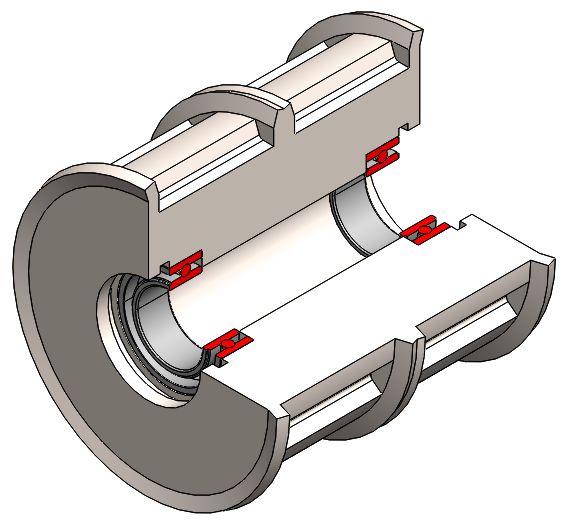
\includegraphics[scale=0.5]{imagenes/Dominio especifico/Validaciones eslabones/PoleaLoca}
	\caption{Vista de secci�n del ocioso con dientes}
	\label{fig:PoleaLoca}
\end{figure}

\textbf{Dise�o de ejes para los eslabones}

\textit{Eje del primer eslab�n}

El primer eje tiene est� configurado por dos apoyos de rodamiento, una polea ociosa doble, una polea s�ncrona com�n y dos sujetadores, como se muestra en la Figura \ref{fig:DEje1}.

\begin{figure}
\centering		
	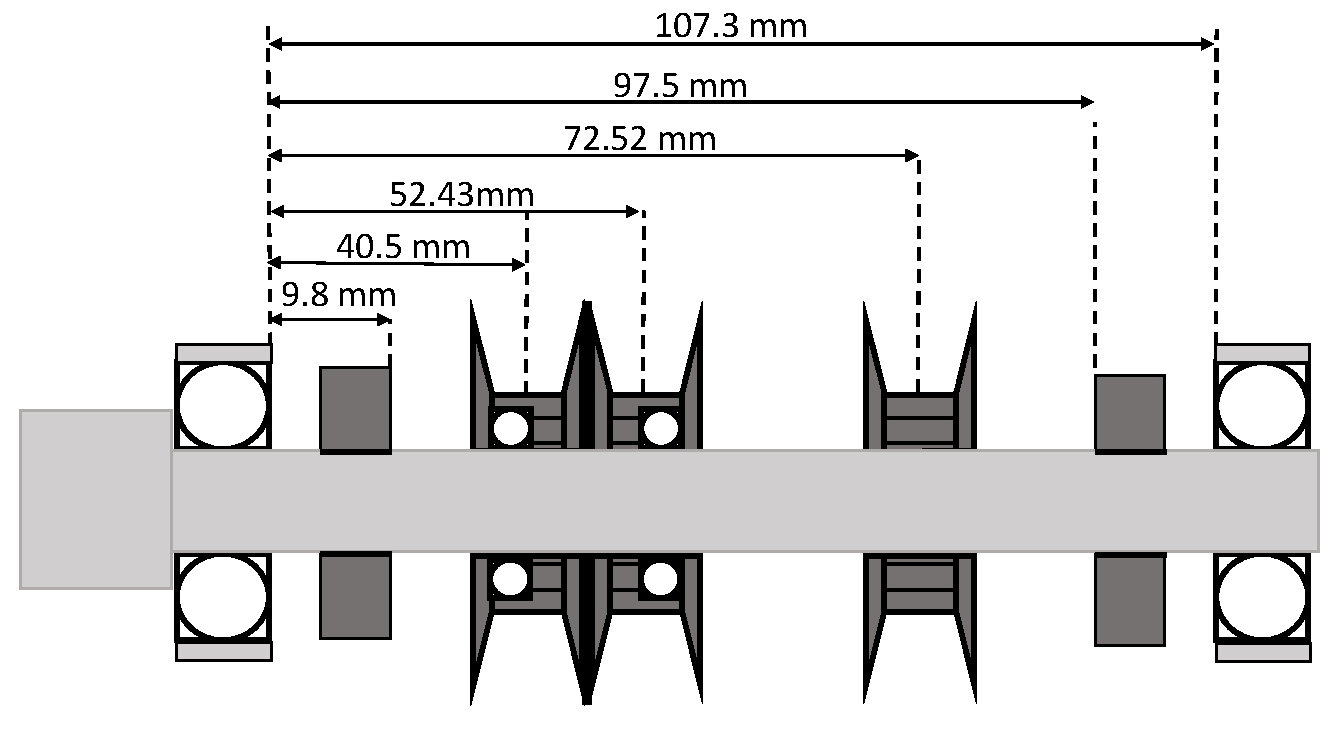
\includegraphics[scale=0.5]{imagenes/Dominio especifico/Validaciones eslabones/Transmision/DiagramaEJE1}
	\caption{Diagramas de cargas del eje 1}
	\label{fig:DEje1}
\end{figure}

Para conocer la magnitud del momento flector y el momento torsionante, se analiza el eje como viga en dos planos, mostrados en las Figuras \ref{fig:CEje1} y \ref{fig:CEje1a}.

\begin{figure}
\centering		
	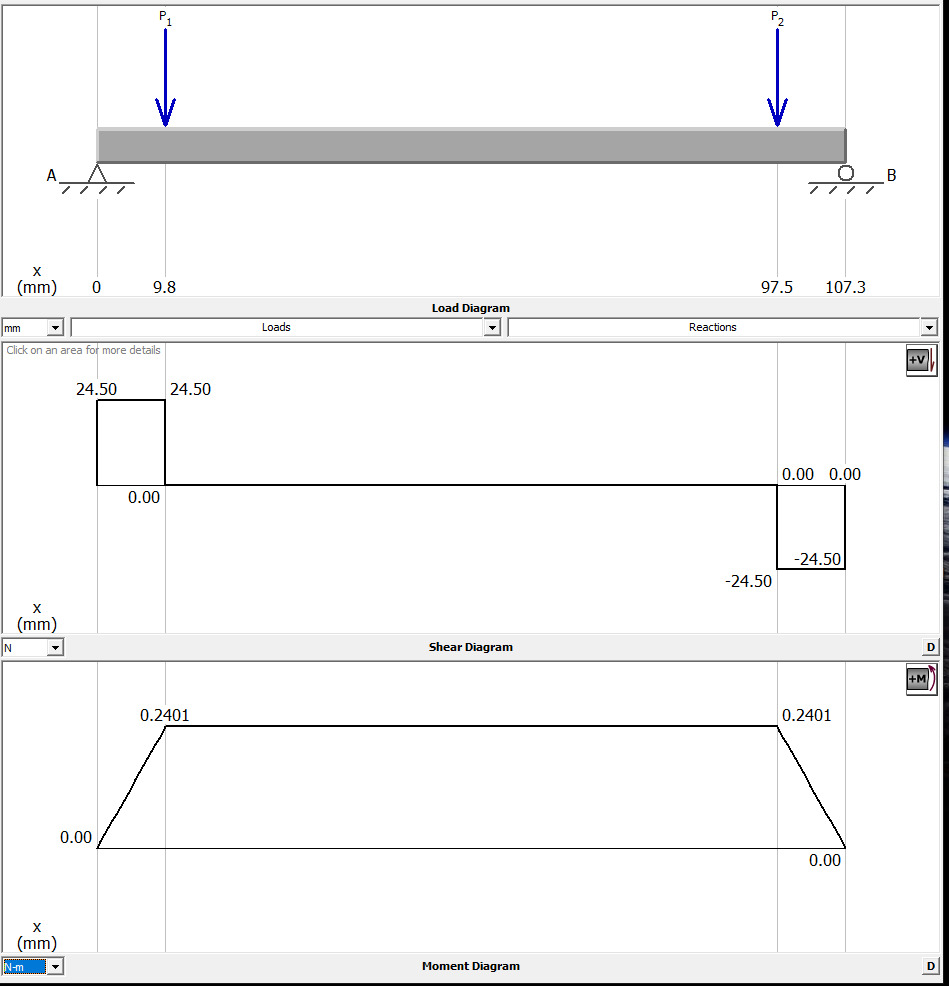
\includegraphics[scale=0.4]{imagenes/Dominio especifico/Validaciones eslabones/Transmision/Eje1f}
	\caption{Plano frontal de cargas del eje 1}
	\label{fig:CEje1}
\end{figure}

\begin{figure}
\centering		
	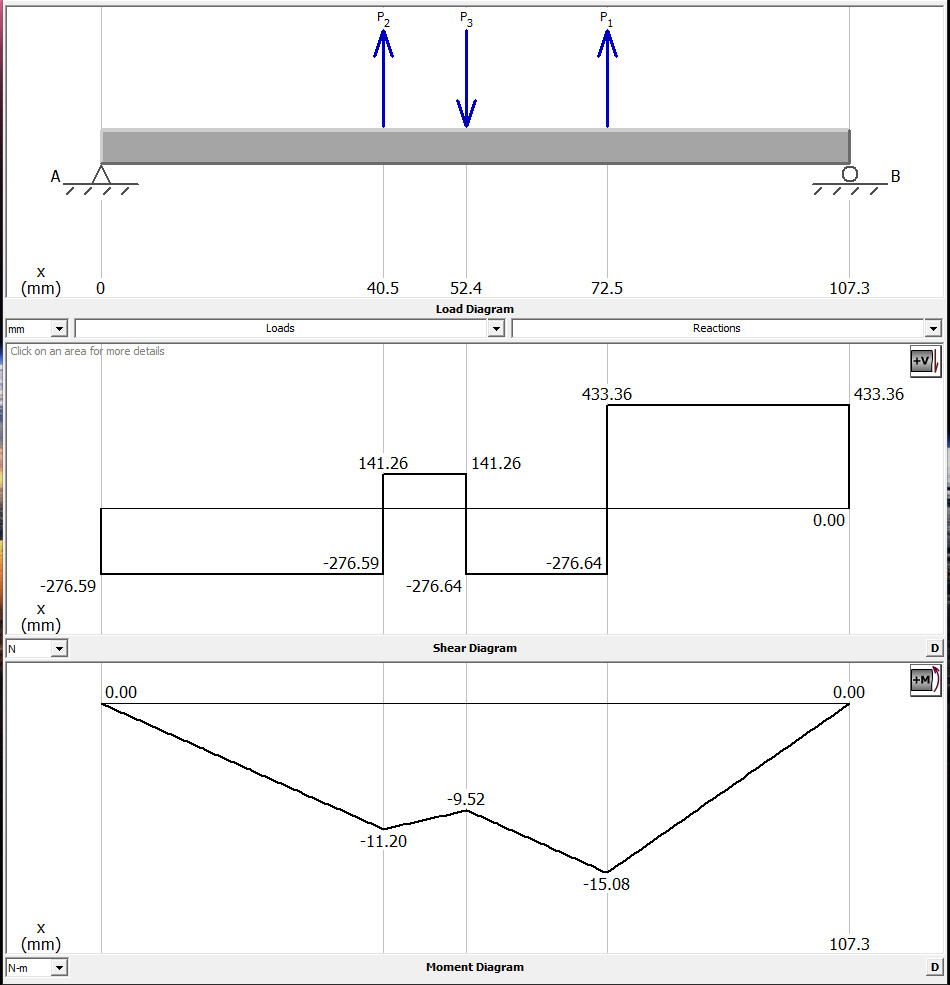
\includegraphics[scale=0.4]{imagenes/Dominio especifico/Validaciones eslabones/Transmision/Eje1s}
	\caption{Plano superior de cargas del eje 1}
	\label{fig:CEje1a}
\end{figure}

De estos diagramas se obtienen adem�s las reacciones generadas en los rodamientos, las cuales se utilizan m�s adelante para realizar la selecci�n de estos.

Para calcular la fuerza que la banda aplica sobre el eje, se utilizan las ecuaciones \ref{eq:FuerzaBanda}.

\begin{align*}
F_{n} &= \frac{11.244Nm}{0.023749m}=473.45N\\
F_{s} &= 1.5*473.45=710.177N
\end{align*}

\begin{align*}
F_{n} &= \frac{6.616Nm}{0.02375m}=278.568N\\
F_{s} &= 1.5*278.568=417.852N
\end{align*}

Con los valores obtenidos, enlistados a continuaci�n, se propone utilizar acero 1060 rolado, cuyas caracter�sticas son:

\begin{itemize}[noitemsep,nolistsep]
\item Densidad: $7850 \unitfrac{Kg}{m^{3}}$
\item M�dulo de elasticidad: $205 GPa$
\item L�mite el�stico: $814 MPa$
\item Esfuerzo de cedencia: $485 MPa$
\end{itemize}

Se ajusta el valor del l�mite el�stico con las ecuaciones \ref{eq:Sn} y \ref{eq:SnC} con los siguientes factores de correcci�n\cite{Mott}

\begin{itemize}[noitemsep,nolistsep]
\item Factor de material: $C_{m} = 0.8$
\item Factor de tipo de esfuerzo (flexionante): $C_{st} = 1$
\item Factor de confiabilidad al 90\%: $C_{R} = 0.9$
\item Factor de tama�o: $C_{s} = 0.95$
\end{itemize}

\begin{align*}
S_{n} &=0.5*814 MPa = 407 MPa\\
S'_{n} &= 407 MPa * 0.8 * 1 *0.9*0.95 = 278 MPa
\end{align*}

Finalmente, con los valores obtenidos, se puede calcular el di�metro m�nimo del primer eje con la ecuaci�n \ref{eq:DiamEje}.

\begin{align*}
D_{1} &= 0.0113 m
\end{align*}

Las reacciones en los apoyos representan las cargas radiales a las que est�n sometidos los rodamientos, por lo que es necesario calcular la carga din�mica m�nima que deben soportar utilizando la ecuaci�n \ref{eq:RodamientosAleados}, tomando como base una vida de un a�o con el servicio intermitente, es decir, 2900 horas o 4.002 millones de revoluciones.

\begin{align*}
C_{eje-1} &= 166.823 N \\
C_{eje-2} &= 160.377 N 
\end{align*}

\textit{Eje del segundo eslab�n}

De manera an�loga al dise�o del primer eje, se analizan las cargas a las que est� sometido el segundo eje, como se muestra en la Figura \ref{fig:DEje2}.

\begin{figure}
\centering		
	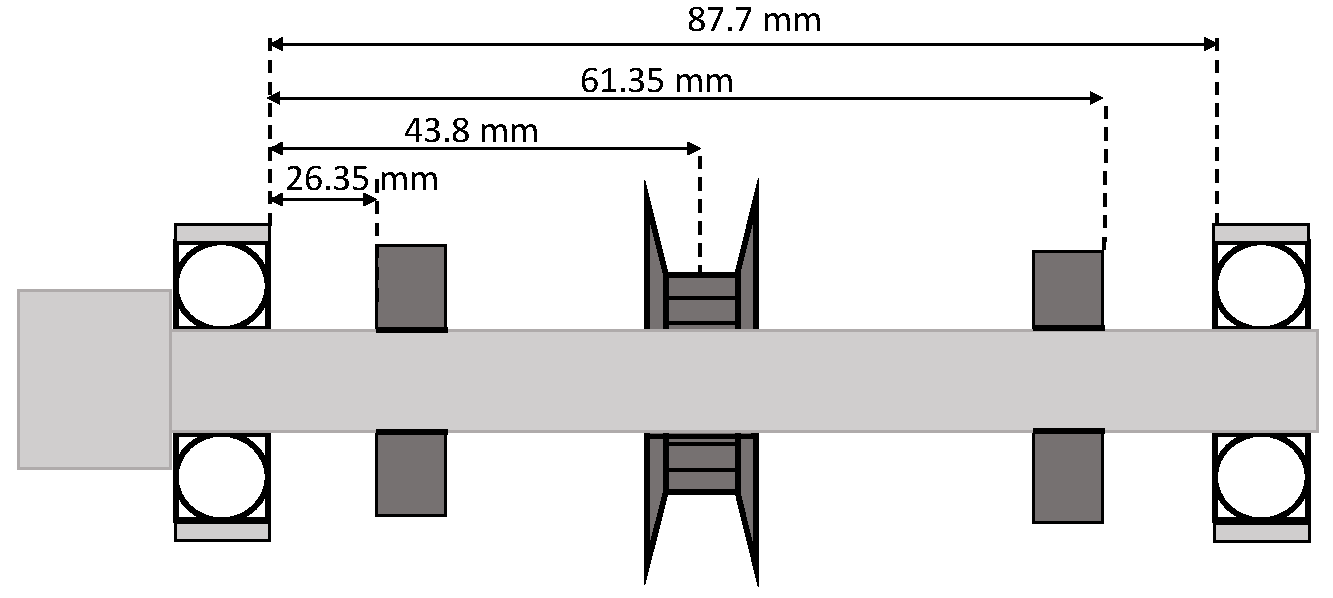
\includegraphics[scale=0.5]{imagenes/Dominio especifico/Validaciones eslabones/Transmision/DiagramaEJE2}
	\caption{Diagramas de cargas del eje 2}
	\label{fig:DEje2}
\end{figure}

Como se puede ver en las Figuras \ref{fig:CEje2}  y \ref{fig:CEje2a}., solo la polea y los eslabones producen fuerzas sobre el eje, el cual tambi�n est� apoyado en dos rodamientos.

\begin{figure}
\centering		
	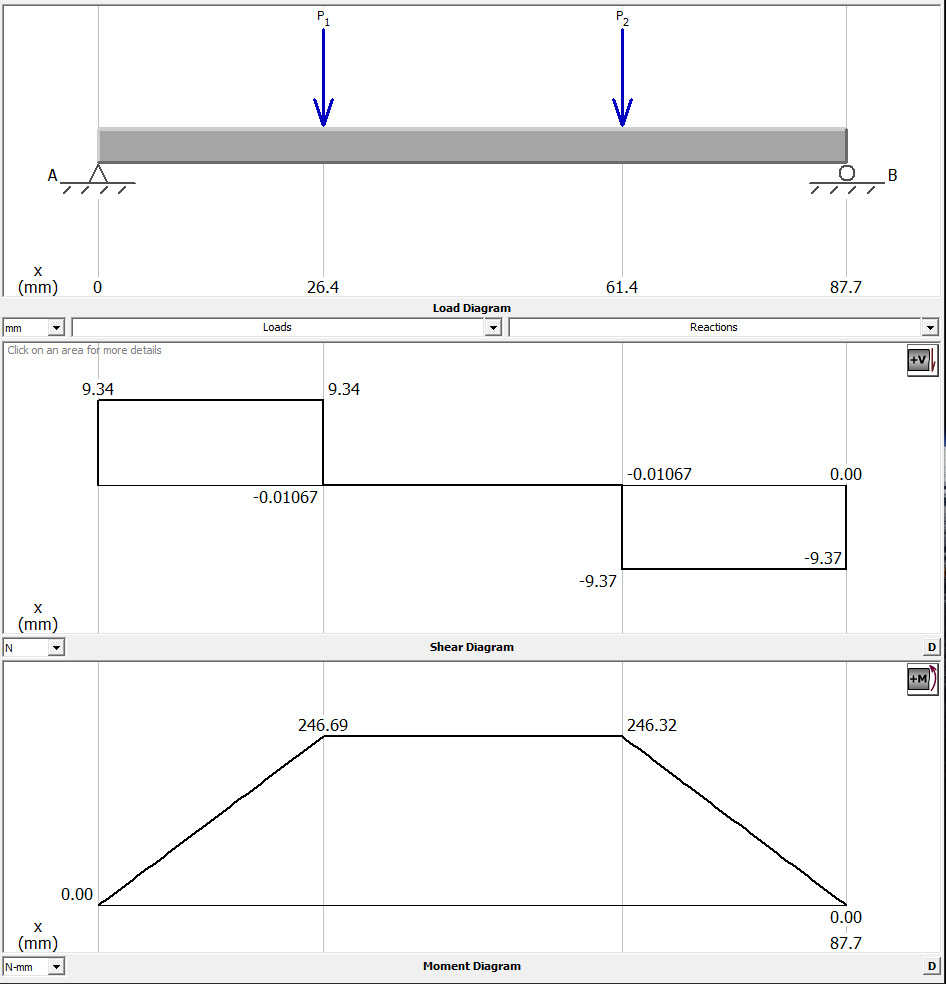
\includegraphics[scale=0.4]{imagenes/Dominio especifico/Validaciones eslabones/Transmision/Eje2f}
	\caption{Plano frontal de cargas del eje 2}
	\label{fig:CEje2}
\end{figure}

\begin{figure}
\centering		
	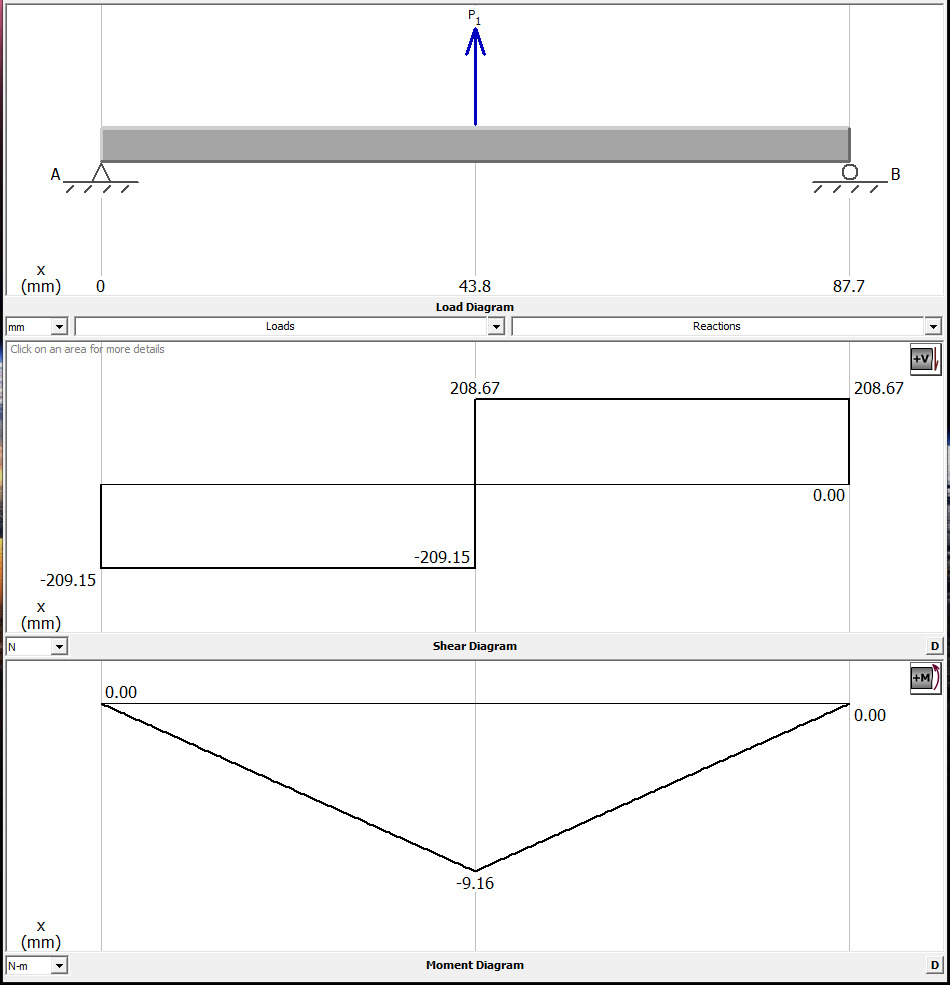
\includegraphics[scale=0.4]{imagenes/Dominio especifico/Validaciones eslabones/Transmision/Eje2s}
	\caption{Plano superior de cargas del eje 2}
	\label{fig:CEje2a}
\end{figure}

La fuerza ejercida por la banda, es la misma que la calculada anteriormente para la polea ociosa.

Para este eje, se propone el mismo material, y se utilizan los mismos factores de correci�n.

Entonces, el di�metro m�nimo queda como sigue:

\begin{align*}
D_{2} &= 0.0096 m
\end{align*}

Finalmente, las reacciones obtenidas se utilizan en la ecuaci�n \ref{eq:RodamientosAleados}

\begin{align*}
C_{1} &= 95.013 N \\
C_{2} &= 95.240 N 
\end{align*}

Las piezas comerciales adquiridas para ensamblar el manipulador, las cuales pueden verse en el Anexo \ref{An:PiezasExtra}, son:

\begin{itemize}[noitemsep,nolistsep]
\item Chumacera de piso: Soporte para el eje del eslab�n perteneciente al segundo GDL.
\item Abrazadera para motor: Sujeci�n de los motores a la base giratoria.
\item Chumacera de pared: Soporte para el eje del eslab�n perteneciente al tercer GDL.
\item Sujetador: Para acoplar r�gidamente el eje al eslab�n.
\end{itemize}

\subsubsection*{Base del manipulador}

En el dise�o de la cadera (GDL 1) se considera extender el eje de giro del motor a una plataforma giratoria que sostenga a los dem�s elementos del manipulador rob�tico. Dicha extensi�n consiste en un acoplador sujeto al eje del motor en un extremo y al eje de la plataforma giratoria en el otro. 

Considerando que el eje de giro se encuentra sometido a cargas y esfuerzos debido a la distribuci�n de los elementos del manipulador rob�tico, se colocan rodamientos en el eje de giro de la plataforma giratoria para resistir las fuerzas axiales y radiales generadas.

Estas cargas se conocen al trasladar las reacciones generadas por el brazo rob�tico y la muestra que transporta hacia las direcciones radial y axial, como se muestra en la Figura \ref{fig:DCBase}, las cuales se distribuyen a rodamientos espec�ficos para cada tipo de carga.

\begin{figure}
\centering		
	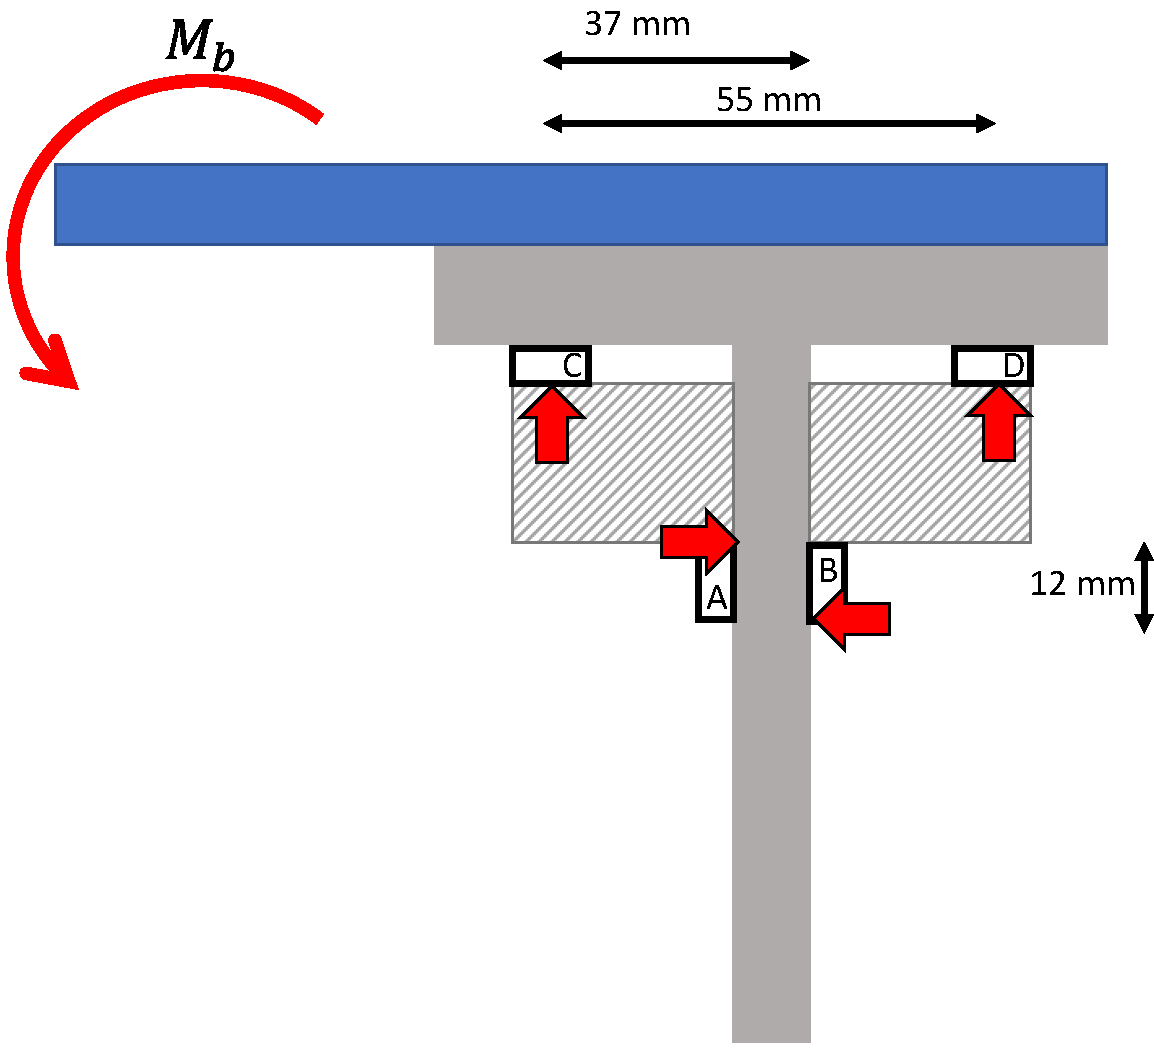
\includegraphics[scale=0.5]{imagenes/Dominio especifico/Validaciones eslabones/Transmision/Diagrama reacciones baleros 2}
	\caption{Diagrama de cargas para el eje}
	\label{fig:DCBase}
\end{figure}

La Tabla \ref{tab:MasasBrazo} muestra las masas de los elementos del brazo, as� como la distancia a la que se encuentran del punto D, que es en el que se realiza la suma de momentos.

\begin{table}
\centering
\caption{Masas de los elementos del brazo rob�tico}
\begin{scriptsize}
\begin{tabular}{|c|c|c|c|}
\hline
                  & \textbf{S�mbolo} & \textbf{Masa {[}kg{]}} & \textbf{Distancia {[}m{]}} \\ \hline
Muestra           & $m_{piedra}$          & 0.5                    & 0.96                       \\ \hline
Efector final     & $m_{ef}$              & 0.5                    & 0.885                      \\ \hline
Mu�eca            & $m_{mu\tilde{n}eca}$          & 0.627                  & 0.775                      \\ \hline
Eslab�n 2         & $m_{2}$               & 0.28                   & 0.535                      \\ \hline
Eslab�n 1         & $m_{1}$               & 0.627                  & 0.255                      \\ \hline
Soporte del brazo & $m_{soporte}$         & 0.5                    & 0.095                      \\ \hline
Base giratoria    & $m_{base}$            & 2.375                  & 0.0275                     \\ \hline
\end{tabular}
\label{tab:MasasBrazo}
\end{scriptsize}
\end{table}

\begin{align*}
R_{A} &= 488.6 N\\
R_{B} &= 488.6 N\\
R_{C} &= 326.58 N\\
R_{D} &= -273.51 N
\end{align*}

Con las reacciones $R_{A}$ y $R_{B}$, es posible dise�ar el eje, pues son las �nicas que provocan flexi�n, mientras que el momento torsionante es proporcionado por el motor.

El material disponible para acoplar el eje del motor, y sobre el cual se aplican las reacciones, es acero inoxidable 303, cuyas caracter�sticas se enlistan a continuaci�n. 

\begin{itemize}[noitemsep,nolistsep]
\item Densidad: $8000 \unitfrac{Kg}{m^{3}}$
\item M�dulo de elasticidad: $193 GPa$
\item L�mite el�stico: $620 MPa$
\item Esfuerzo de cedencia: $240 MPa$
\end{itemize}

El proceso de dise�o del eje es similar al de los ejes de los eslabones, como se muestra:

\begin{align*}
S_{n} &=0.5*620 MPa = 310 MPa \\
S'_{n} &= 310 MPa * 0.8 * 1 *0.9*0.95 = 212 MPa \\
D &= 0.0178 m \\
C_{axial} &= 496 N \\
C_{radial} &= 742 N 
\end{align*}

Las cargas din�micas que son capaces de soportar los rodamientos se calculan con la ecuaci�n \ref{eq:RodamientosAleados}, sustituyendo $P_{d}$ con el valor de las reacciones axial y radial seg�n sea el caso.

De acuerdo al cat�logo en l�nea del fabricante SKF\cite{SKF}, se seleccionan los rodamientos m�s peque�os que cumplen con las caracter�sticas necesarias, siendo un rodamiento axial de agujas con designaci�n AXK-4565 (Anexo \ref{An:RodAx}) para las cargas axiales, y un rodamiento de rodillos con designaci�n NU-303 (Anexo \ref{An:RodRad}) para las cargas radiales.

La plataforma giratoria debe ser capaz de sostener a los dos motores que mueven los eslabones, as� como el soporte del brazo. Por ello se utiliza una geometr�a de medio c�rculo en la parte posterior, mientras que en la parte frontal se colocan dos salientes, como se muestra en la Figura \ref{fig:PlataGiratoria}, sobre los que se montan las chumaceras que soportan al eje del primer grado de libertad, dejando un espacio libre entre estas para permitir que el eslab�n gire por debajo del plano horizontal evitando la colisi�n con la plataforma. Para facilitar la comprensi�n de la geometr�a, se recurre a una perspectiva isom�trica y a la vista superior, mostradas en la Figura \ref{fig:PlataformaVistas}.

\begin{figure}
\centering		
	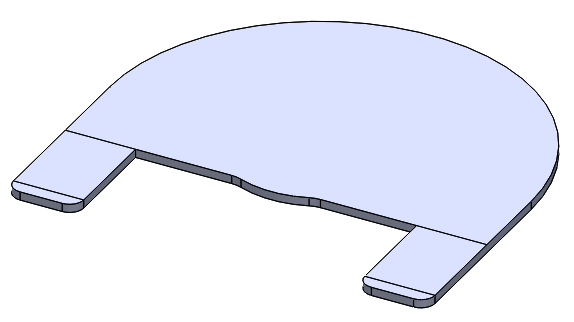
\includegraphics[scale=0.5]{imagenes/Dominio especifico/Validaciones eslabones/Mesa/Plataforma}
	\caption{Modelo CAD de la plataforma giratoria}
	\label{fig:PlataGiratoria}
\end{figure}

\begin{figure}
\centering		
	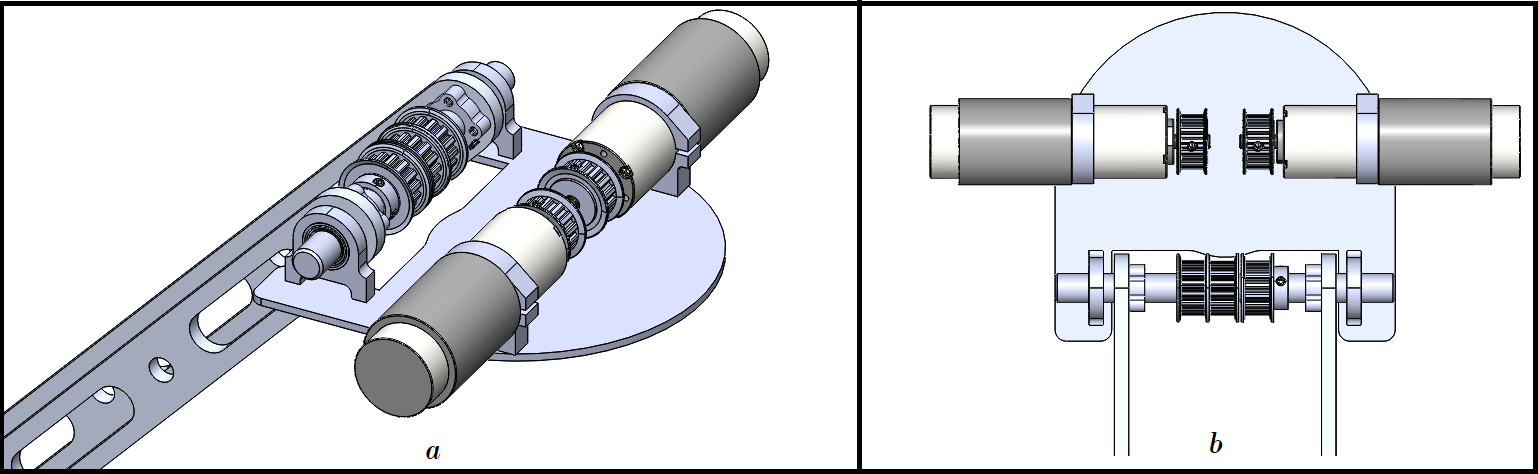
\includegraphics[scale=0.4]{imagenes/Dominio especifico/Validaciones eslabones/Mesa/Plataforma_Vistas}
	\caption{Vistas de referencia para la plataforma giratoria}
	\label{fig:PlataformaVistas}
\end{figure}

El cilindro est� dise�ado de acuerdo a las dimensiones del eje del motor acoplado y los rodamientos seleccionados previamente, adem�s de a�adir barrenos para atornillarlo a la base fija, 
cuyo resultado se muestra en la Figura \ref{fig:CilindroFijo}.

\begin{figure}
\centering		
	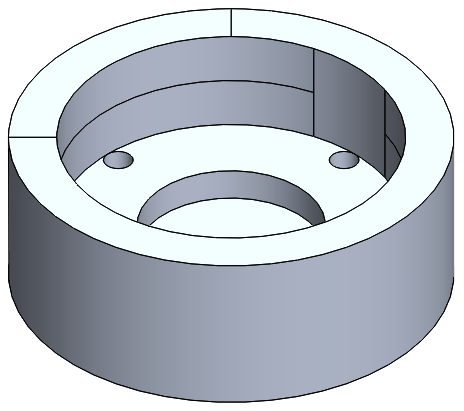
\includegraphics[scale=0.5]{imagenes/Dominio especifico/Validaciones eslabones/Mesa/CilindroFijo}
	\caption{Modelo CAD del cilindro base}
	\label{fig:CilindroFijo}
\end{figure}

Finalmente, la base fija, mostrada en la Figura \ref{fig:BaseFija}, es aquella que debe soportar los esfuerzos generados por todo el manipulador, en la que se acopla el cilindro base de la Figura \ref{fig:CilindroFijo} a la placa, como se muestra en la Figura \ref{fig:CilindroBase}.

\begin{figure}
\centering		
	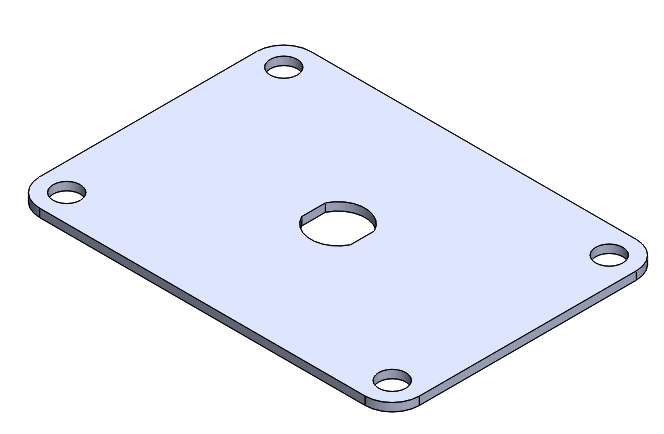
\includegraphics[scale=0.5]{imagenes/Dominio especifico/Validaciones eslabones/Mesa/BaseFija}
	\caption{Modelo CAD de la base fija del manipulador}
	\label{fig:BaseFija}
\end{figure}

\begin{figure}
\centering		
	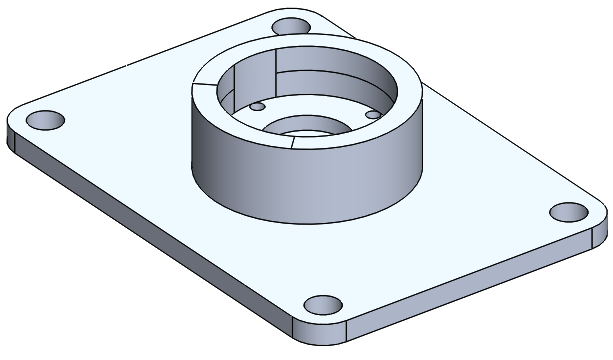
\includegraphics[scale=0.5]{imagenes/Dominio especifico/Validaciones eslabones/Mesa/Cilindro-Base}
	\caption{Cilindro base acoplado a la base fija}
	\label{fig:CilindroBase}
\end{figure}

\subsubsection*{Validaci�n de la base}

Para comprobar la integridad mec�nica de las piezas que conforman la base, se realiza un an�lisis de elemento finito\cite{FEASolid} en SolidWorks\textregistered, utilizando como material el aluminio 6061 (propiedades disponibles en la Tabla \ref{tab:PropiedadesAluminio}).

\textit{Plataforma giratoria}

Para la plataforma giratoria, que tiene una masa de 0.128[Kg], el an�lisis queda como sigue:

La Figura \ref{fig:PlatGirEsfuerzos} muestra que el esfuerzo von Mises m�ximo es 53.73[MPa], por lo que tiene un factor de seguridad de 5.11. Mientras que la Figura \ref{fig:PlatGirDef} muestra que la deformaci�n m�xima es 0.8[mm].

\begin{figure}
\centering		
	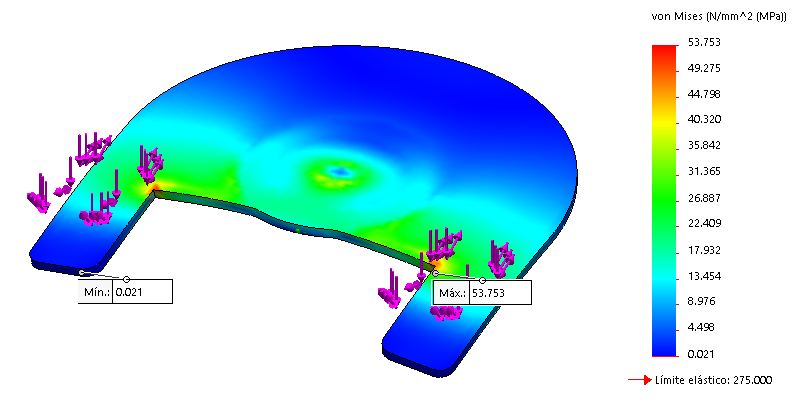
\includegraphics[scale=0.7]{imagenes/Dominio especifico/Validaciones eslabones/Mesa/Plataforma_Analisis}
	\caption{An�lisis est�tico de resistencia de la plataforma giratoria}
	\label{fig:PlatGirEsfuerzos}
\end{figure}

\begin{figure}
\centering		
	\includegraphics[scale=0.7]{imagenes/Dominio especifico/Validaciones eslabones/Mesa/Plataforma_Deformacion}
	\caption{An�lisis est�tico de rigidez de la plataforma giratoria}
	\label{fig:PlatGirDef}
\end{figure}

\textit{Cilindro base}

Para el cilindro base, que tiene una masa de 0.096[Kg], el an�lisis es el siguiente:

La Figura \ref{fig:CilBaseEsfuerzos} muestra que el esfuerzo von Mises m�ximo es 52[MPa], por lo que tiene un factor de seguridad de 5.28. Mientras que la Figura \ref{fig:CilBaseDef} muestra que la deformaci�n m�xima es 0.004[mm].

\begin{figure}
\centering		
	\includegraphics[scale=0.7]{imagenes/Dominio especifico/Validaciones eslabones/Mesa/CilindroFijo_Analisis}
	\caption{An�lisis est�tico de resistencia del cilindro base}
	\label{fig:CilBaseEsfuerzos}
\end{figure}

\begin{figure}
\centering		
	\includegraphics[scale=0.7]{imagenes/Dominio especifico/Validaciones eslabones/Mesa/CilindroFijo_Deformacion}
	\caption{An�lisis est�tico de rigidez del cilindro base}
	\label{fig:CilBaseDef}
\end{figure}

\textit{Base fija}

Para la base fija, que tiene una masa de .230[Kg], el an�lisis queda como sigue:

La Figura \ref{fig:CilindroBaseEsfuerzos} muestra que el esfuerzo von Mises m�ximo es 19.9[MPa], por lo que tiene un factor de seguridad de 13.18. Mientras que la Figura \ref{fig:CilindroBaseDef} muestra que la deformaci�n m�xima es 0.028[mm].

\begin{figure}
\centering		
	\includegraphics[scale=0.7]{imagenes/Dominio especifico/Validaciones eslabones/Mesa/Cilindro-Base_Analisis}
	\caption{An�lisis est�tico de resistencia de la base fija}
	\label{fig:CilindroBaseEsfuerzos}
\end{figure}

\begin{figure}
\centering		
	\includegraphics[scale=0.7]{imagenes/Dominio especifico/Validaciones eslabones/Mesa/Cilindro-Base_Deformacion}
	\caption{An�lisis est�tico de rigidez de la base fija}
	\label{fig:CilindroBaseDef}
\end{figure}

\subsubsection*{Dise�o final de la base fija}

La Figura \ref{fig:MesaCAD} muestra la configuraci�n final de la mesa ensamblada, mientras que la Figura \ref{fig:MesaExplosionada} muestra una vista explosionada que permite apreciar los elementos que la conforman.

\begin{figure}
\centering		
	\includegraphics[scale=0.5]{imagenes/Dominio especifico/Validaciones eslabones/Mesa/VistaIso}
	\caption{Modelo CAD de la base del manipulador}
	\label{fig:MesaCAD}
\end{figure}

\begin{figure}
\centering		
	\includegraphics[scale=0.5]{imagenes/Dominio especifico/Validaciones eslabones/Mesa/Mesa explosionada}
	\caption{Vista explosionada del modelo CAD de la base del manipulador}
	\label{fig:MesaExplosionada}
\end{figure}

\subsubsection*{Mu�eca esf�rica}

De acuerdo a las ecuaciones \ref{eq:DesCin} y \ref{eq:DesCin2}, para poder realizar el desacoplamiento cinem�tico los 3 ejes de giro de la mu�eca deben intersecarse en un punto, por lo que se dise�a una mu�eca esf�rica.

Debido a que se cuenta con poco espacio y son f�ciles de utilizar, se propone utilizar servomotores de tama�o est�ndar.

Con la finalidad de acoplar el servomotor al segundo eslab�n, y para soportar los esfuerzos radiales, se utiliza una estructura de carga comercial que, como puede apreciarse en la vista explosionada de la Figura \ref{fig:MuneMot1Exp}, consta de dos soportes laterales, un marco para el servomotor, una chumacera y un adaptador para el eje del mismo. La estructura armada se muestra en la Figura \ref{fig:PrimerMotor}.

\begin{figure}
  \centering
  \begin{minipage}[b]{0.4\textwidth}
\begin{figure}[H]
\centering		
	\includegraphics[scale=0.5]{imagenes/Dominio especifico/Muneca/Primer motor Exp}
	\caption{Vista explosionada de la estructura de carga del primer grado de libertad de la mu�eca}
	\label{fig:MuneMot1Exp}
\end{figure}
\end{minipage}
  \hfill
  \begin{minipage}[b]{0.4\textwidth}
\begin{figure}[H]
\centering		
	\includegraphics[width=\textwidth]{imagenes/Dominio especifico/Muneca/Primer motor}
	\caption{Estructura de carga ensamblada}
	\label{fig:PrimerMotor}
\end{figure}    
  \end{minipage}
\end{figure}

Para soportar los motores restantes, manteniendo la intersecci�n de sus ejes, se dise�an varias piezas como sigue:

\begin{itemize}[noitemsep,nolistsep]
\item Un conector tipo C que transmite la rotaci�n del primer GDL.
\item Una pieza a modo de cubierta que sostiene a los servomotores manteniendo la ortogonalidad entre sus ejes de giro, a la vez que absorbe las cargas radiales aplicadas al eje a trav�s de rodamientos.
\item Una tapa para la cubierta con espacio para rodamiento radial, adem�s de un cople para unir el eje del tercer servomotor con la base del efector final.
\end{itemize}

Adem�s, se adquieren dos acopladores el eje de de los servomotores de los �ltimos 2 GDL de la mu�eca. Aunado a ello, se adquieren dos rodamientos con di�metro intero igual al di�metro del acoplador de 1/2 [in] y un rodamiento con brida para acoplar la pieza con forma de ``C''. 

Estas piezas pueden observarse a detalle en la Figura \ref{fig:Motor23Exp}, mientras que el ensamble se muestra en la Figura \ref{fig:Motor23}. Las piezas adquiridas se encuentran en el Anexo \ref{An:PiezasMueca}, mientras que los rodamientos aparecen en el Anexo \ref{An:RodChi}.

\begin{figure}
\centering
\begin{minipage}[b]{0.4\textwidth}
\begin{figure}[H]
\centering		
	\includegraphics[width=\textwidth]{imagenes/Dominio especifico/Muneca/Segundo y tercer motor EXP}
	\caption{Vista explosionada de la estructura del segundo y tercer GDL}
	\label{fig:Motor23Exp}
\end{figure}
\end{minipage}
\hfill
\begin{minipage}[b]{0.4\textwidth}
\begin{figure}[H]
\centering		
	\includegraphics[width=\textwidth]{imagenes/Dominio especifico/Muneca/Segundo y tercer motor}
	\caption{Estructura del segundo y tercer GDL ensamblada}
	\label{fig:Motor23}
\end{figure}
\end{minipage}
\end{figure}

La mu�eca esf�rica completa con los servomotores se puede apreciar en la Figura \ref{fig:MuneCAD}.

\begin{figure}
\centering		
	\includegraphics[scale=0.5]{imagenes/Dominio especifico/Muneca/MunecaCompleta}
	\caption{Modelo CAD de la mu�eca esf�rica}
	\label{fig:MuneCAD}
\end{figure}

Debido a que estas piezas presentan geometr�as complejas, y que no se someten a esfuerzos tan grandes como el brazo, se opta por utilizar manufactura aditiva con materiales t�picos de la misma. En este sentido, los m�s populares son el PLA y el ABS, sin embargo, el PLA es conocido por su fragilidad, por lo que el material seleccionado es ABS.

Finalmente, resta seleccionar los servomotores a usar, para lo cual se calcula el par m�ximo que deben de soportar, utilizando los diagramas mostrados en las Figuras \ref{fig:ParMuneca1} y \ref{fig:ParMuneca1}, destacando que, dado que las cargas se encuentran muy cerca del eje de giro del tercer GDL, el momento que generan es muy peque�o, por lo que se omite su c�lculo.

\begin{figure}
  \centering
  \begin{minipage}[b]{0.4\textwidth}
\begin{figure}[H]
\centering		
	\includegraphics[width=\textwidth]{imagenes/Dominio especifico/Muneca/Muneca1}
	\caption{Reacci�n m�xima para el primer grado de libertad de la mu�eca}
	\label{fig:ParMuneca1}
\end{figure}
\end{minipage}
  \hfill
  \begin{minipage}[b]{0.4\textwidth}
\begin{figure}[H]
\centering		
	\includegraphics[width=\textwidth]{imagenes/Dominio especifico/Muneca/Muneca2}
	\caption{Reacci�n m�xima para el segundo grado de libertad de la mu�eca}
	\label{fig:ParMuneca2}
\end{figure}    
  \end{minipage}
\end{figure}

Conociendo este valor, se comparan los distintos motores disponibles en el mercado, utilizando un �rbol de decisiones (Ap�ndice \ref{ApA2:Servo}) y, con base en este, se selecciona el servo de alto rendimiento de EzRobot, con las siguientes caracter�sticas:

\begin{itemize}[noitemsep,nolistsep]
\item Par m�ximo a 7.4[V] = 19 [Kg cm]
\item Corriente a motor bloqueado = 3[A]
\item Voltaje de operaci�n = 4.8[V] a 8.4[V]
\end{itemize}

\subsection{M�dulo de efector (M2)}

La funci�n f1.3 (``Tomar/dejar muestra''), requiere que exista una herramienta en el extremo del manipulador rob�tico, capaz de sujetar una piedra con las caractaer�sticas determinadas en los requerimientos R1, R2, R3 y R4. 
De acuerdo al concepto soluci�n seleccionado, el efector final a desarrollar es de tipo ``Gripper'' de tres dedos. 

Existe un modelo de efector con esas caracter�sticas, desarrollado por Kuat Telegenov, Yedige Tlegenov y Almas Shintemirov, titulado y publicado en IEEE Access con el nombre ``A Low-Cost Open-Source 3-D-Printed
Three-Finger Gripper Platform for Research
and Educational Purposes''\cite{GripperOS}, el cual, como se presenta en el abstract del art�culo: ``Presentamos un modelo de plataforma de gripper rob�tico de tres dedos de fuente abierta (Open source) para prop�sitos de educaci�n e investigaci�n'', resulta una opci�n viable para utilizar en este proyecto.

La acci�n de agarre de las falanges se basa en un mecanismo subactuado de dos grados de libertad. En la Figura \ref{fig:MecGrip} se muestra un diagrama esquem�tico de los elementos del mecanismo. 

\begin{figure}
\centering		
	\includegraphics[scale=0.3]{imagenes/MecanismoGripper}
	\caption{Elementos del mecanismo del gripper, IEEE}
	\label{fig:MecGrip}
\end{figure}

El torque de un actuador se aplica en $O_{1}$, donde el torque $T_{a}$ genera un desplazamiento angular $\theta_{1}$. El resorte con m�dulo el�stico $K$, ejerce una fuerza que mantiene el �ngulo $\theta_{2}$ fijo. Cuando el eslab�n $O_{1}-O_{2}$ se ve detenido en su movimiento, el torque $T_{a}$ provoca una elongaci�n en el resorte, lo que provoca un movimiento angular en $\theta_{2}$. Dicha secuencia es mostrada en la Figura \ref{fig:SecGrip}.

\begin{figure}
\centering		
	\includegraphics[scale=0.3]{imagenes/SecuenciaGripper}
	\caption{Secuencia de movimientos del mecanismo del gripper, IEEE}
	\label{fig:SecGrip}
\end{figure}

En la Figura \ref{fig:Grip1D} se muestra el ensamblaje de una falange con el mecanismo de actuaci�n, que consiste en un tornillo sin fin m�s un engrane que transmite el movimiento al pi��n que, unido al eslab�n, transmite el torque al mecanismo.

\begin{figure}
\centering		
	\includegraphics[scale=0.3]{imagenes/DedoYEngranes}
	\caption{Ensamblaje de una falange del gripper, IEEE}
	\label{fig:Grip1D}
\end{figure}

Seg�n los resultados de las pruebas mostradas en la fuente\cite{GripperOS}, el efector es capaz de sujetar objetos con diversas geometr�as. En la Figura \ref{fig:Balonxd}, el lector puede observar que el objeto agarrado es una pelota de geometr�a esf�rica. Se busca que el agarre para la muestra de roca sea similar, sin embargo, la pelota tiene dimensiones mayores al tama�o propuesto en el requerimiento R2, como se puede apreciar en el diagrama simplificado mostrado en la Figura \ref{fig:EFDSOri}, por lo que se propone un cambio de dimensiones en los ``dedos'' y la plataforma que funciona como ``palma''.

\begin{figure}
\centering		
	\includegraphics[scale=0.5]{imagenes/Balonxd}
	\caption{Agarre del gripper con una pelota esf�rica, IEEE}
	\label{fig:Balonxd}
\end{figure}

\begin{figure}
\centering		
	\includegraphics[scale=0.25]{imagenes/Dominio especifico/Efector/Original1}
	\caption{Diagrama simplificado de un dedo y la muestra objetivo}
	\label{fig:EFDSOri}
\end{figure}

Despu�s de realizar un an�lisis geom�trico con el software Geogebra\textregistered , y comprobar varias opciones, se determinan las siguientes dimensiones:

\begin{itemize}[noitemsep,nolistsep]
\item Distancia del eje central de la palma al inicio de la falange: 2.5[cm]
\item Longitud de la primer falange: 6[cm]
\item Longitud de la segunda falange: 2.5[cm]
\end{itemize}

Con las dimensiones modificadas se aprecia que, aunque la palma no tenga contacto con la muestra, existe una mejora en el agarre de la misma, a la vez que se disminuye la probabilidad de golpear el suelo al disminuir la distancia necesaria para asegurar la sujeci�n. Esto se puede apreciar en la Figura \ref{fig:EFDSMod}.

\begin{figure}
\centering		
	\includegraphics[scale=0.25]{imagenes/Dominio especifico/Efector/Modificado1}
	\caption{Diagrama simplificado de un dedo y la muestra objetivo}
	\label{fig:EFDSMod}
\end{figure}

La distribuci�n de los dedos del efector se pueden apreciar claramente en la vista superior del efector, mostrada en la Figura \ref{fig:EFDistDedos}, mientras que el mecanismo subactuado se aprecia en la Figura \ref{fig:EFDistMec}.

\begin{figure}[H]
\begin{minipage}[b]{0.4\textwidth}
\begin{figure}[H]
\centering		
	\includegraphics[width=\textwidth]{imagenes/Dominio especifico/Efector/Efector superior}
	\caption{Distribuci�n de los dedos del efector}
	\label{fig:EFDistDedos}
\end{figure}
\end{minipage}
\hfill
\begin{minipage}[b]{0.4\textwidth}
\begin{figure}[H]
\centering		
	\includegraphics[width=\textwidth]{imagenes/Dominio especifico/Efector/Efector lateral}
	\caption{Mecanismo subactuado del efector}
	\label{fig:EFDistMec}
\end{figure}
\end{minipage}
\end{figure}

Adem�s de la modificaci�n a las dimensiones, se agrega una placa deslizante que permite introducir un sensor de fuerza para determinar cuando la muestra es asegurada, de manera que no se ejerza una fuerza excesiva que resulte en un da�o a la muestra o al efector, como se muestra en la Figura \ref{fig:EfectorSensores}.

\begin{figure}
\centering		
	\includegraphics[scale=0.4]{imagenes/Dominio especifico/Efector/Acoplamiento sensores}
	\caption{Ensamble de sensor de presi�n en la falange del efector}
	\label{fig:EfectorSensores}
\end{figure}

Para medir la fuerza ejercida por el efector a la muestra se opta por utilizar sensores de fuerza resistivos, ya que el espacio disponible para colocar el sensor es limitado y la delgadez de estos sensores los convierte en una opci�n adecuada.

El espacio est� pensado para adaptarse a sensores de aproximadamente media pulgada de di�metro, por lo que el sensor FSR 402 (Anexo \ref{An:SFuerza}) es apropiado para los objetivos del proyecto.

Para transmitir la potencia al tornillo sin fin que act�a las falanges, se utiliza un buje de servo, mostrado en el Anexo \ref{An:BujeEfector}.

El efector ensamblado se puede apreciar en la Figura \ref{fig:EFEnsamble}, y las piezas que lo componen en la vista explosionada de la Figura \ref{fig:EFExp}.

\begin{figure}[H]
\begin{minipage}[b]{0.4\textwidth}
\begin{figure}[H]
\centering		
	\includegraphics[width=1.2\textwidth]{imagenes/Dominio especifico/Efector/EfectorConActuador}
	\caption{Ensamble final del efector}
	\label{fig:EFEnsamble}
\end{figure}
\end{minipage}
\hfill
\begin{minipage}[b]{0.4\textwidth}
\begin{figure}[H]
\centering		
	\includegraphics[width=\textwidth]{imagenes/Dominio especifico/Efector/EfectorConActuadorEXP}
	\caption{Vista explosionada del efector}
	\label{fig:EFExp}
\end{figure}
\end{minipage}
\end{figure}

\subsubsection*{Validaci�n del efector redise�ado}

Para comprobar que el efector tiene un rango de agarre por encima y debajo de la muestra ideal de [5cm] de di�metro, se realiza un an�lisis geom�trico con piezas de 3[cm] y 7[cm], como se puede observar en la Figuras \ref{fig:EFV1} y \ref{fig:EFV2}.

\begin{figure}[H]
\begin{minipage}[b]{0.4\textwidth}
\begin{figure}[H]
\centering		
	\includegraphics[width=1.5\textwidth]{imagenes/Dominio especifico/Efector/Modificado2}
	\caption{An�lisis geom�trico del agarre del efector con muestra de 3[mm] de di�metro}
	\label{fig:EFV1}
\end{figure}
\end{minipage}
\hfill
\begin{minipage}[b]{0.4\textwidth}
\begin{figure}[H]
\centering		
	\includegraphics[width=1.5\textwidth]{imagenes/Dominio especifico/Efector/Modificado3}
	\caption{An�lisis geom�trico del agarre del efector con muestra de 7[mm] de di�metro}
	\label{fig:EFV2}
\end{figure}
\end{minipage}
\end{figure}

\subsection{Modelo matem�tico del sistema rob�tico}

\subsubsection*{Modelo cinem�tico}

\subsubsection*{Cinem�tica directa}

Para abordar el problema de cinem�tica directa, primeramente se establecen marcos coordenados, que sirven como referencia para la posici�n y orientaci�n de cada eslab�n, de acuerdo a la convenci�n de Denavit-Hartenberg \cite{Spong}, como se ve en la Figura \ref{fig:AsigMarcos}.

\begin{figure}
\centering		
	\includegraphics[scale=0.35]{imagenes/Dominio especifico/AsignacionMarcos}
	\caption{Asignaci�n de los marcos de referencia a las articulaciones del robot}
	\label{fig:AsigMarcos}
\end{figure}

Para determinar la relaci�n de posici�n y orientaci�n del marco de referencia del efector final respecto al marco fijo $T_{0}^{6}$, se utilizan las matrices de transformaci�n homog�nea $A_{i}$, que relacionan la posici�n y orientaci�n del marco de referencia $i$ respecto al marco $i-1$, construidas con la ecuaci�n \ref{eq:MTH}.

\begin{table}
\centering
\caption{Par�metros de Denavit-Hartenberg}
\begin{scriptsize}
\begin{tabular}{|c|c|c|c|c|c|}
\hline
$i$  & $\theta$ & $d$  & $a$  & $\alpha$ & Offset \\ \hline
1  & $\theta_{1}$    & $o_{ff_{1}}$ & $o_{ff_{2}}$ & $\frac{\pi}{2}$  & 0      \\ \hline
2  & $\theta_{2}$    & 0  & $l_{1}$ & 0     & 0      \\ \hline
2' & $\theta_{3}$    & 0  & $l_{2}$ & $\frac{\pi}{2}$  & 0      \\ \hline
3  & $-\frac{\pi}{2}$ & 0  & 0  & $-\frac{\pi}{2}$ & 0      \\ \hline
4  & $\theta_{4}$    & 0  & 0  & $\frac{\pi}{2}$  & $\pi$     \\ \hline
5  & $\theta_{5}$    & 0  & 0  & $\frac{\pi}{2}$  & $\pi$     \\ \hline
6  & $\theta_{6}$    & $l_{3}$ & 0  & 0     & 0      \\ \hline
\end{tabular}
\end{scriptsize}
\label{tab:PDH}
\end{table}


Al sustituir los valores de los par�metros de Denavit-Hartenberg, indicados en la Tabla \ref{tab:PDH}, es posible calcular las matrices de transformaci�n homog�nea $A_{1}$ hasta $A_{6}$, las cuales, al posmultiplicarse, resultan en la matriz $T_{0}^{6}$:

\begin{figure}
\centering
	\begin{minipage}[b]{0.3\textwidth}
		$$
		A_{1} = 
		\begin{bmatrix}
		c_{1} & 0 & s_{1} & O_{2}c_{1}\\
		s_{1} & 0 & -c_{1} & O_{2}s_{1}\\
		0 & 1 & 0 & O_{1}\\
		0 & 0 & 0 & 1
		\end{bmatrix}
		$$
	\end{minipage}
	\hfill
	\begin{minipage}[b]{0.3\textwidth}
		$$
		A_{2} = 
		\begin{bmatrix}
		c_{2} & -s_{2} & 0 & l_{1}c_{2}\\
		s_{2} & c_{2} & 0 & l_{1}s_{2}\\
		0 & 0 & 1 & 0\\
		0 & 0 & 0 & 1
		\end{bmatrix}
		$$
	\end{minipage}
	\hfill
	\begin{minipage}[b]{0.3\textwidth}
		$$ 
		A_{2}' = 
		\begin{bmatrix} 
		c_{3} & 0 & s_{3} & l_{2}c_{3} \\
		s_{3} & 0 & -c_{3} & l_{2}s_{3} \\ 
		0 & 1 & 0 & 0 \\ 
		0 & 0 & 0 & 1 
		\end{bmatrix} 
		$$
	\end{minipage}
\end{figure}

\begin{figure}
	\small
	\centering
	\begin{minipage}[b]{0.2\textwidth}
		$$
		A_{3}  = 
		\begin{bmatrix} 
		0 & 0 & 1 & 0 \\ 
		-1 & 0 & 0 & 0 \\ 
		0 & -1 & 0 & 0 \\ 
		0 & 0 & 0 & 1 
		\end{bmatrix}  
		$$
	\end{minipage}
	\hfill
	\begin{minipage}[b]{0.2\textwidth}
		$$ 
		A_{4} = 
		\begin{bmatrix} 
		-c_{4} & 0 & -s_{4} & 0 \\ 
		-s_{4} & 0 & c_{4} & 0 \\ 
		0 & 1 & 0 & 0 \\ 
		0 & 0 & 0 & 1 
		\end{bmatrix}
		$$
	\end{minipage}
	\hfill
	\begin{minipage}[b]{0.2\textwidth}
		$$
		A_{5} = 
		\begin{bmatrix} 
		-c_{5} & 0 & -s_{5} & 0 \\
		-s_{5} & 0 & c_{5} & 0 \\
		0 & 1 & 0 & 0 \\ 
		0 & 0 & 0 & 1 
		\end{bmatrix}
		$$
	\end{minipage}
	\hfill
	\begin{minipage}[b]{0.2\textwidth}
		$$
		A_{6} = 
		\begin{bmatrix}
		c_{6} & -s_{6} & 0 & 0\\
		s_{6} & c_{6} & 0 & 0\\
		0 & 0 & 1 & l_{3}\\
		0 & 0 & 0 & 1\\
		\end{bmatrix}
		$$
	\end{minipage}
\end{figure}

\subsubsection*{Validaci�n del modelo cinem�tico}
A forma de comprobaci�n, los par�metros de Denavit-Hartenberg obtenidos se colocan en el toolbox \textit{``Robotics''} para MATLAB\textregistered , desarrollado por Peter Corke para simular sistemas rob�ticos (el c�digo puede encontrarse en el Ap�ndice \ref{Ap:CodigoRoboCorke}), en el que se construye un modelo tridimensional del sistema en desarrollo, mostrado en la Figura \ref{fig:RoboCorke}, en donde se puede observar que la configuraci�n formada por los par�metros de la Tabla \ref{tab:PDH} son congruentes con la configuraci�n de la asignaci�n de marcos de la Figura \ref{fig:AsigMarcos}. 

\begin{figure}
\centering		
	\includegraphics[scale=0.5]{imagenes/Dominio especifico/Validaciones eslabones/ROBOTNPG}
	\caption{Modelo tridimensional del sistema rob�tico desarrollado en el toolbox Robotics de Peter Corke para MATLAB\textregistered}
	\label{fig:RoboCorke}
\end{figure}


\subsubsection*{Cinem�tica inversa}

Debido a que este manipulador rob�tico se compone de un brazo articulado de codo planar y una mu�eca esf�rica, se aprovecha la capacidad que ofrece de desarrollar la cinem�tica inversa del brazo y la mu�eca por separado, lo que se conoce como \textit{desacoplamiento cinem�tico}.

\textbf{Cinem�tica inversa del brazo articulado - Posici�n inversa.}

Para conocer los valores de las juntas pertenecientes al brazo articulado, es conveniente utilizar un enfoque geom�trico, proyectando el centro de la mu�eca esf�rica. La Figura  \ref{fig:ProyT1} muestra la proyecci�n del centro de la mu�eca en el plano $x_{0}-y_{0}$, permitiendo ver f�cilmente el valor de $\theta_{1}$ como una relaci�n entre las coordenadas $x_{c}$ y $y_{c}$ del centro de la mu�eca, como se muestra en la ecuaci�n \ref{eq:T1}.

\begin{figure}
\centering		
	\includegraphics[scale=0.3]{imagenes/Dominio especifico/Validaciones eslabones/EsquemaT1.pdf}
	\caption{Proyecci�n del centro de la mu�eca en el plano $x_{0}-y_{0}$}
	\label{fig:ProyT1}
\end{figure}

\begin{equation}
\label{eq:T1}
\theta_{1}=atan2\left(x_{c},y_{c}\right) 
\end{equation}

\begin{flushleft}
En donde: $ \; \theta_{1} =$ Valor de la variable del primer grado de libertad.
%\\
%\\
%$\qquad \quad \qquad \rho_{e} \: \; =$ Densidad del eslab�n.
\end{flushleft}

Para encontrar el valor de $\theta_{2}$ y $\theta_{3}$, resulta de gran utilidad la Figura \ref{fig:ProyT2T3}.

\begin{figure}
\centering		
	\includegraphics[scale=0.3]{imagenes/Dominio especifico/Validaciones eslabones/EsquemaT2T3.pdf}
	\caption{Proyecci�n del centro de la mu�eca en el plano formado por los eslabones}
	\label{fig:ProyT2T3}
\end{figure}

En primer lugar, es importante considerar que existen dos desplazamientos entre las juntas como sigue:


\begin{align*}
r_{real} &= r_{total}-o_{ff_{2}} \\
s &= z_{c}-o_{ff{1}}
\end{align*}


Utilizando el teorema de Pit�goras, se calcula la longitud equivalente $l_{eq}$, para posteriormente obtener $\theta_{3}$ mediante la ley de cosenos.

\begin{align*}
l_{eq} &= \sqrt{r_{real}^{2}+s_{2}}\\
\cos \theta_{3} &= \frac{l_{eq}^{2}-l_{1}^{2}-l_{2}^{2}}{2l_{1}l_{2}}\\
&= \frac{(r-o_{ff_{2}})^{2} + s^{2} - l_{1}^{2} - l_{2}^{2}}{2l_{1}l_{2}}\\
&= \frac{(x_{c}^2 + y_{c}^2 -o_{ff_{2}})^{2} + (z_{c}-o_{ff{1}})^{2} - l_{1}^{2} - l_{2}^{2}}{2l_{1}l_{2}}:=D
\end{align*}

Dado que $ l_{eq}^{2} = (x_{c}^2 + y_{c}^2 -o_{ff_{2}})^{2} $ y $ s^{2} = z_{c}-o_{ff{1}} $. Entonces, $ \theta_{3} $ est� dada por la ecuaci�n \ref{eq:T3}.

\begin{align}
\label{eq:T3}
\theta_{3} &= atan2\left(D,\pm\sqrt{1-D^{2}}\right)
\end{align}

\begin{align*}
\textrm{En donde:}\\
\theta_{3} &= \textrm{Valor de la variable del tercer grado de libertad.}
\end{align*}


El hecho de que se tomen ambas ra�ces en la ecuaci�n implica que son soluciones para la posici�n de \textbf{codo arriba} y \textbf{codo abajo}, para lo que finalmente se obtiene $ \theta_{2} $, definido por la ecuaci�n \ref{eq:T2}.


\begin{align*}
\theta_{2} &= atan2\left(r_{real},s\right) - atan2\left(l_{1} + l_{2}c_{3}, l_{2}s_{3}\right)
\end{align*} 

\begin{align}
\label{eq:T2}
\theta_{2} &= atan2\left(\sqrt{x_{c}^2 + y_{c}^2 -o_{ff_{2}}}, z_{c}-o_{ff{1}}\right) - atan2\left(l_{1} + l_{2}c_{3}, l_{2}s_{3}\right)
\end{align}

\begin{align*}
\textrm{En donde:}\\
\theta_{2} &= \textrm{Valor de la variable del segundo grado de libertad.}
\end{align*}

\textbf{Cinem�tica inversa de la mu�eca esf�rica - Orientaci�n inversa.}

Para obtener los tres grados de libertad faltantes, pertenecientes a la orientaci�n de la mu�eca, resulta �til resolver la ecuaci�n \ref{eq:R06Pieper}.

La matriz simb�lica $R_{6}^{3}$ es la siguiente:

%\label{eq:R36Sim}
\begin{align*}
R_{6}^{3} = 
\left[
\begin{array}{ccc}
c_{4} c_{5} c_{6}-s_{4} s_{6} & -s_{4} c_{6}-s_{6} c_{4} c_{5} & s_{5} c_{4} \\
s_{4} c_{5} c_{6}+s_{6} c_{4} & c_{4} c_{6}-s_{4} s_{6} c_{5} & s_{4} s_{5} \\
-s_{5}c_{6} & s_{5} s_{6} & c_{5}
\end{array}
\right]
\end{align*}

\begin{align}
\label{eq:R03}
R_{3}^{0} = 
\left[
\begin{array}{ccc}
-s_{1} & -s_{23} c_{1} & c_{1} c_{23} \\
c_{1} & -s_{1} s_{23} & s_{1} c_{23} \\
0 & c_{23} & s_{23}
\end{array}
\right]
\end{align}

Para construir $\left(R_{3}^{0}\right)^{T}R$ se utiliza la ecuaci�n \ref{eq:RTarget} y \ref{eq:R03}, resultando en:

\begin{align*}
R_{6}^{3} &= 
\left[
\begin{array}{ccc}
r_{21} c_{1}-r_{11} s_{1} & 
r_{22} c_{1}-r_{12} s_{1} &
r_{23} c_{1}-r_{13} s_{1} \\
-r_{11} s_{23} c_{1}-r_{21} s_{1} s_{23}+r_{31} c_{23} &
-r_{12} s_{23} c_{1}-r_{22} s_{1} s_{23}+r_{32} c_{23} &
-r_{13} s_{23} c_{1}-r_{23} s_{1} s_{23}+r_{33} c_{23} \\
r_{11} c_{1} c_{23}+r_{21} s_{1} c_{23}+r_{31} s_{23} &
r_{12} c_{1} c_{23}+r_{22} s_{1} c_{23}+r_{32} s_{23} &
r_{13} c_{1} c_{23}+r_{23} s_{1} c_{23}+r_{33} s_{23}
\end{array}
\right]
\end{align*}

Resolviendo para $\theta_{4}$, $\theta_{5}$ y $\theta_{6}$ como sigue.

\begin{align}
\label{eq:T5}
\theta_{5} &= atan2\left(
r_{13}c_{1}c_{23}+r_{23}s_{1}c_{23}+r_{33}s_{23},
\pm\sqrt{1-\left(r_{13}c_{1}c_{23}+r_{23}s_{1}c_{23}+r_{33}s_{23}\right)^{2}}
\right)
\end{align}

\begin{align}
\label{eq:T4}
\theta_{4} &= atan2\left(
\pm\sqrt{s_{5}^{2}-\left(r_{33}c_{23}-r_{13}c_{1}s_{23}-r_{23}s_{1}s_{23}\right)^{2}},
r_{33}c_{23}-r_{13}c_{1}s_{23}-r_{23}s_{1}s_{23}
\right)
\end{align}

\begin{align}
\label{eq:T6}
\theta_{6} &= atan2\left(
\pm\sqrt{s_{5}^{2}-\left(r_{12}c_{1}c_{23}+r_{22}s_{1}c_{23}+r_{32}s_{23}\right)^{2}},
r_{12}c_{1}c_{23}+r_{22}s_{1}c_{23}+r_{32}s_{23}
\right)
\end{align}

\subsubsection*{Jacobiano}

En esta secci�n se derivan las relaciones de velocidad entre las velocidades lineal y angular del efector final con respecto a las velocidades de las juntas.

\begin{figure}
	\centering
	\begin{minipage}[b]{\textwidth}
		\begin{align*}
		J_{1} = 
		\left[
		\begin{array}{c}
		-l_1 s_{1} c_{2}-l_2 s_{1} c_{23}-l_3 \left(s_{1} c_{23} c_{5}+s_{5} \left(c_{1} c_{4}-s_{1} s_{23} s_{4}\right)\right)-O_2 s_{1} \\
		l_1 c_{1} c_{2}+l_2 c_{1} c_{23}+l_3 \left(c_{1} c_{23} c_{5}-s_{5} \left(s_{1} c_{4}+c_{1} s_{23} s_{4} \right)\right)+O_2 c_{1} \\
		0 \\
		0 \\
		0 \\
		1
		\end{array}
		\right]
		\end{align*}
	\end{minipage}
	\hfill
	\begin{minipage}[b]{0.3\textwidth}
		\begin{align*}
		J_{2} =
		\left[
		\begin{array}{c}
		-c_{1} \left(l_1 s_{2}+l_3 s_{4} s_{5} c_{23}+s_{23} \left(l_3 c_{5}+l_2\right)\right) \\
		-s_{1} \left(l_1 s_{2}+l_3 s_{4} s_{5} c_{23}+s_{23} \left(l_3 c_{5}+l_2\right)\right) \\
		l_1 c_{2} -l_3 s_{23} s_{4} s_{5}+c_{23} \left(l_3 c_{5}+l_2\right) \\
		s_{1} \\
		-c_{1} \\
		0 
		\end{array}
		\right]
		\end{align*}
	\end{minipage}
	\hfill
	\begin{minipage}[b]{0.3\textwidth}
		\begin{align*}
			J_{3} =
			\left[
			\begin{array}{c}
			 -c_{1} \left(l_3 s_{4} s_{5} c_{23}+s_{23} \left(l_3 c_{5}+l_2\right)\right) \\
			 -s_{1} \left(l_3 s_{4} s_{5} c_{23}+s_{23} \left(l_3 c_{5}+l_2\right)\right) \\
			 -l_3 s_{4} s_{5} s_{23} + c_{23} \left(l_3 c_{5}+l_2\right) \\
			 s_{1} \\
			 -c_{1} \\
			 0 
			 \\
			\end{array}
			\right]
		\end{align*}
	\end{minipage}
	\hfill
	\begin{minipage}[b]{0.3\textwidth}
		\begin{align*}
			J_{4} =
			\left[
			\begin{array}{c}
			 l_3 s_{5} \left(s_{1} s_{4} - c_{1} s_{23} c_{4}\right) \\
			 -l_3 s_{5} \left(c_{1} s_{4} + s_{1} s_{23} c_{4}\right) \\
			 l_3 s_{5} c_{23} c_{4} \\
			 c_{1} c_{23} \\
			 s_{1} c_{23} \\
			 s_{23} 
			\end{array}
			\right]
		\end{align*}
	\end{minipage}
	\hfill
	\begin{minipage}[b]{0.4\textwidth}
		\begin{align*}
			J_{5} =
			\left[
			\begin{array}{c}
			 -l_3 \left(s_{1} c_{4} c_{5}+c_{1} \left(s_{23} s_{4} c_{5}+s_{5} c_{23}\right)\right) \\
			 l_3 \left(c_{1} c_{4} c_{5}-s_{1} \left(s_{23} s_{4} c_{5}+s_{5} c_{23}\right)\right) \\
			 l_3 \left(s_{4} c_{23} c_{5}-s_{23} s_{5}\right) \\
			 s_{1} s_{4} - c_{1} s_{23} c_{4} \\
			 -c_{1}s_{4} - s_{1} s_{23} c_{4} \\
			 c_{23} c_{4} 
			\end{array}
			\right]
		\end{align*}
	\end{minipage}
	\hfill
	\begin{minipage}[b]{0.4\textwidth}
		\begin{align*}
			J_{6} =
			\left[
			\begin{array}{c}
			 0 \\
			 0 \\
			 0 \\
			 c_{1} c_{23} c_{5}-s_{5} \left(s_{1} c_{4}+c_{1} s_{23} s_{4} \right) \\
			 s_{1} c_{23} c_{5}+s_{5} \left(c_{1} c_{4}-s_{1} s_{23} s_{4}\right) \\
			 s_{23} c_{5}+s_{4} s_{5} c_{23} 
			\end{array}
			\right]
		\end{align*}
	\end{minipage}
\end{figure}


\begin{align}
\label{eq:Jacobiano}
J = \left[ \begin{array}{c|c|c|c|c|c}
J_{1} & J_{2} & J_{3} & J_{4} & J_{5} & J_{6}
\end{array} \right]
\end{align}

\textbf{Jacobiano para singularidades}

Con el fin de realizar el desacoplamiento de singularidades, se construye un Jacobiano de la forma:

\begin{align}
J_{i} &= \begin{bmatrix}
 z_{i-1} \times (o_{3}-o_{i-1})\\   z_{i-1} 
\end{bmatrix}
\label{eq:JacSing}
\end{align}

Las singularidades se calculan con la ecuaci�n \ref{eq:detJ}, quedando como sigue:

\begin{align}
\label{eq:ArmSing}
det J_{11} = -l_1 l_2 s_{3} \left(l_1 c_{2}+l_2 c_{23}+O_2\right)
\end{align}

\begin{align}
\label{eq:WristSing}
det J_{22} = -s_{5}
\end{align}

De \ref{eq:ArmSing}, se puede observar que las singularidades del brazo se presentan cuando

\begin{align*}
\theta_{3} &= 0\\
l_1 c_{2}+l_2 c_{23}+O_2 &= 0
\end{align*}

Mientras que de \ref{eq:WristSing} se obtiene la singularidad de la mu�eca esf�rica, que se presenta cuando

\begin{align*}
\theta_{5} &= 0\\
\end{align*}

Lo que implica que dos de sus ejes est�n alineados, provocando que el Jacobiano pierda rango y existan infinitas soluciones para un solo valor de posici�n.

\subsection*{Modelo din�mico}

%Poner vinculo al marco te�rico
Como se menciona en el marco te�rico, el Jacobiano adecuado\cite{Spong} para el modelo din�mico se calcula sustituyendo la longitud total $l$ del eslab�n del GDL de inter�s por la distancia de su origen a su centro de masa $l_c$, y volviendo cero las columnas correspondientes a los GDL posteriores.\footnote{$J_{v \omega 6}$ es igual al Jacobiano calculado en la ecuaci�n \ref{eq:Jacobiano}, pues toma en cuenta el movimiento de todas las juntas, por lo que solo se requiere sustituir $l_3$ por $l_{c3}$}

\begin{figure}
	\centering
	\begin{minipage}{0.4\textwidth}
		\begin{align*}
			J_{v \omega 1} = 
			\begin{bmatrix}
			 -O_2 s_{1} & 0 & 0 & 0 & 0 & 0 \\
			 O_2 c_{1} & 0 & 0 & 0 & 0 & 0 \\
			 0 & 0 & 0 & 0 & 0 & 0 \\
			 0 & 0 & 0 & 0 & 0 & 0 \\
			 0 & 0 & 0 & 0 & 0 & 0 \\
			 1 & 0 & 0 & 0 & 0 & 0 
			\end{bmatrix}
			\end{align*}		
	\end{minipage}
	\hfill
	\begin{minipage}{0.4\textwidth}
		\begin{align*}
			J_{v \omega 2} = 
			\begin{bmatrix}
			 -s_{1} \left(l_{c1} c_{2}+O_2\right) & -l_{c1} s_{2} c_{1} & 0 & 0 & 0 & 0 \\
			 c_{1} \left(l_{c1} c_{2}+O_2\right) & -l_{c1} s_{1} s_{2} & 0 & 0 & 0 & 0 \\
			 0 & l_{c1} c_{2} & 0 & 0 & 0 & 0 \\
			 0 & s_{1} & 0 & 0 & 0 & 0 \\
			 0 & -c_{1} & 0 & 0 & 0 & 0 \\
			 1 & 0 & 0 & 0 & 0 & 0 
			\end{bmatrix}
			\end{align*}
		\end{minipage}
		\hfill
		\begin{minipage}{0.4\textwidth}
			\begin{align*}
				J_{v \omega 3} &= 
				\begin{bmatrix}
				-s_{1} \left(l_1 c_{2}+l_{c2} c_{23}+O_2\right) & -c_{1} \left(l_1 s_{2}+l_{c2} s_{23}\right) & -l_{c2} s_{23} c_{1} & 0 & 0 & 0 \\
				c_{1} \left(l_1 c_{2}+l_{c2} c_{23}+O_2\right) & -s_{1} \left(l_1 s_{2}+l_{c2} s_{23}\right) & -l_{c2} s_{1} s_{23} & 0 & 0 & 0 \\
				0 & l_1 c_{2}+l_{c2} c_{23} & l_{c2} c_{23} & 0 & 0 & 0 \\
				0 & s_{1} & s_{1} & 0 & 0 & 0 \\
				0 & -c_{1} & -c_{1} & 0 & 0 & 0 \\
				1 & 0 & 0 & 0 & 0 & 0 
				\end{bmatrix}
			\end{align*}
		\end{minipage}
		\hfill
		\begin{minipage}{0.4\textwidth}
			\begin{align*}	
				J_{v \omega 4} = 
				\begin{bmatrix}
				-s_{1} \left(l_1 c_{2}+l_2 c_{23}+O_2\right) & -c_{1} \left(l_1 s_{2}+l_2 s_{23}\right) & -l_2 s_{23} c_{1} & 0 & 0 & 0 \\
				c_{1} \left(l_1 c_{2}+l_2 c_{23}+O_2\right) & -s_{1} \left(l_1 s_{2}+l_2 s_{23}\right) & -l_2 s_{1} s_{23} & 0 & 0 & 0 \\
				0 & l_1 c_{2}+l_2 c_{23} & l_2 c_{23} & 0 & 0 & 0 \\
				0 & s_{1} & s_{1} & c_{1} c_{23} & 0 & 0 \\
				0 & -c_{1} & -c_{1} & s_{1} c_{23} & 0 & 0 \\
				1 & 0 & 0 & s_{23} & 0 & 0 
				\end{bmatrix}
			\end{align*}
		\end{minipage}
		\hfill
		\begin{minipage}{0.4\textwidth}
			\begin{align*}
				J_{v \omega 5} = 
				\begin{bmatrix}
				-s_{1} \left(l_1 c_{2}+l_2 c_{23}+O_2\right) & -c_{1} \left(l_1 s_{2}+l_2 s_{23}\right) & -l_2 s_{23} c_{1} & 0 & 0 & 0 \\
				c_{1} \left(l_1 c_{2}+l_2 c_{23}+O_2\right) & -s_{1} \left(l_1 s_{2}+l_2 s_{23}\right) & -l_2 s_{1} s_{23} & 0 & 0 & 0 \\
				0 & l_1 c_{2}+l_2 c_{23} & l_2 c_{23} & 0 & 0 & 0 \\
				0 & s_{1} & s_{1} & c_{1} c_{23} & s_{1} s_{4}-s_{23} c_{1} c_{4} & 0 \\
				0 & -c_{1} & -c_{1} & s_{1} c_{23} & -s_{1} s_{23} c_{4} -s_{4} c_{1} & 0 \\
				1 & 0 & 0 & s_{23} & c_{23} c_{4} & 0 
				\end{bmatrix}
			\end{align*}
		\end{minipage}
\end{figure}

\subsection*{Generaci�n de trayectorias}
Para la generaci�n de las trayectorias Home-Muestra-Laboratorio se propone utilizar un polinomio de grado 5, ya que permite restringir los valores iniciales y finales de posici�n, velocidad y aceleraci�n, a diferencia de los polinomios c�bicos, que no permiten restringir la aceleraci�n, generando una sacudida que afecta la precisi�n del manipulador y un pico de corriente que puede afectar los circuitos controladores.

El polinomio de quinto orden 

\begin{align*}
q(t) = a_0+a_1t+a_2t^2+a_3t^3+a_4t^4+a_5t^5
\end{align*}

Sin embargo, es importante tomar en cuenta que el movimiento del robot est� restringido por el espacio en el que se monta, por lo que es necesario tomar en cuenta los obst�culos presentes en el espacio de trabajo, as� como restringir movimientos que provoquen la superposici�n de los eslabones para evitar colisiones.

Finalmente, para la trayectoria Laboratorio-Home, se propone utilizar un m�todo Teach and Play, pues el punto de inicio y el final son conocidos y no es necesario calcular la cinem�tica inversa cada vez que se ejecute.

\subsection*{Control}
Un enfoque t�pico para controlar sistemas rob�ticos es considerar cada junta como un sistema de control independiente que intenta seguir su trayectoria de manera precisa. Sin embargo, esto representa un reto complicado debido a perturbaciones debidas a la gravedad, velocidades y aceleraciones producidas por el resto de las juntas, as� como la fricci�n en cada junta. Por esta raz�n, se propone utilizar una t�cnica de control por juntas independientes, la cual sigue un m�todo sencillo que consiste en representar la inercia del sistema mediante una aproximaci�n denominada ``Inercia efectiva'', que es un promedio de los posibles valores de inercia que el sistema puede adoptar de acuerdo a las configuraciones dentro del espacio de trabajo. A pesar de que dicha aproximaci�n no representa la inercia real, el hecho de presentar una relaci�n de reducci�n alta incrementa la viabilidad en su implementaci�n.

\section{Sistema de Informaci�n (S2)}
\subsection{M�dulo de percepci�n (M3)}

\subsubsection*{Condiciones de operaci�n}

Para asegurar que el sistema trabaja en condiciones seguras de operaci�n, es necesario determinar los par�metros del ambiente, para que el sistema se desactive en cuando alguno de ellos no cumpla con los valores establecidos por los requerimientos (R11 y R12).

Dado que el sistema debe operar a la intemperie, es necesario conocer las condiciones de temperatura y humedad a las que est� expuesto, para ello se recurre a un sensor.

En el mercado hay una gran variedad de productos disponibles capaces de medir estas dos magnitudes, destacando entre ellos el DHT11 (Anexo \ref{An:DHT11}) por su popularidad, lo que lo convierte en un componente de f�cil adquisici�n y uso, y dado que su rango de operaci�n cumple con los requerimientos, es seleccionado.

Los puntos del sistema m�s vulnerables al calentamiento por radiaci�n solar, aire caliente por convecci�n, o por calentamiento propio son: los actuadores, los circuitos electr�nicos y el sistema de alimentaci�n, por lo que deben ser monitoreados.

\subsubsection*{Visi�n artificial}

El objetivo de la visi�n artificial es obtener las coordenadas de la muestra en el espacio.
Para ello se recurre a dos herramientas muy �tiles en el campo de la visi�n por computadora, las cuales son la \textit{homograf�a} y la \textit{estereopsis}.

Se requieren dos im�genes, una vez obtenidas, se realiza la correcci�n de perspectiva a trav�s de la homograf�a, obteniendo una vista superior del suelo, con lo que es posible conocer las coordenadas $x,y$ de la muestra, mientras que, para calcular la profundidad en el eje $z$, se utiliza la estereopsis con ayuda de un diagrama como el de la Figura \ref{fig:DiagramaEstereo}.

La selecci�n de c�maras se realiza de acuerdo al �rbol de decisiones mostrado en el Anexo \ref{An:Cam}.

De los 2 modelos restantes, se selecciona la c�mara m�s econ�mica, pues ambas cumplen con los requerimientos m�nimos, con especificaciones en el Ap�ndice \ref{ApA4:Camara}.

Para la implementaci�n de este algortimo, se propone utilizar software libre, siendo seleccionado el lenguaje de programaci�n Python, con la biblioteca OpenCV, la cual est� orientada a la visi�n por computadora.

\subsection{M�dulo de comunicaci�n (M4)}

Dado que el sistema involucra varios agentes que intercambian datos entre s�, es necesario identificar la forma en que interact�an. Esta interacci�n est� ilustrada en la Figura \ref{fig:ComDiag}. Debido a que estos componentes forman parte de diferentes sistemas, la uni�n de ellos se realiza en el cap�tulo ``Integraci�n''.

\begin{figure}
\centering		
	\includegraphics[scale=0.5]{imagenes/Dominio especifico/Comunicacion/Comunicacion diagrama}
	\caption{Diagrama de comunicaci�n entre m�dulos}
	\label{fig:ComDiag}
\end{figure}

Con ayuda de este diagrama, se determinan los requerimientos de comunicaci�n, mostrados en la Tabla \ref{Tab:ElementosComunicacion}, que ser�n �tiles para dise�ar los circuitos y elegir el microcontrolador adecuado.

\subsubsection*{Comunicaci�n interna}

Los componentes electr�nicos deben interactuar entre s� para lograr que el sistema mecatr�nico realice su funci�n, en la Tabla \ref{Tab:ElementosComunicacion} se muestra la forma en que cada uno de ellos maneja su informaci�n.

\begin{table}
\centering
\caption{Requerimientos de comunicaci�n}
\begin{scriptsize}
\begin{tabular}{|c|c|c|}
\hline
Elemento                   & Numero de terminales & Tipo      \\ \hline
Servomotor (x5)            & 1                    & PWM       \\ \hline
Motor CD (x3)              & 1                    & PWM       \\ \hline
Encoder (x3)               & 2                    & Digital   \\ \hline
Sensor de temperatura (x3) & 1                    & 1-wire    \\ \hline
M�dulo de celda de carga   & 1                    & Serial    \\ \hline
Sensores de fuerza (x3)    & 1                    & Anal�gico \\ \hline
Camara (x2)                & 2                    & SPI       \\ \hline
Computadora                & 2                    & UART      \\ \hline
\end{tabular}
\end{scriptsize}
\label{Tab:ElementosComunicacion}
\end{table}

\subsubsection*{Comunicaci�n con el usuario}

Para interactuar con el usuario, se plantea utilizar una interfaz gr�fica, como la que se ve en la Figura \ref{fig:FrontEnd}.

Como se puede ver, esta interfaz cuenta con los siguientes elementos.

\begin{itemize}[noitemsep,nolistsep]
\item Bot�n de activaci�n y desactivaci�n, adem�s cuando se cierre la aplicaci�n se realiza la comprobaci�n del estado del sistema, si se encuentra activo, env�a el brazo a la posici�n de reposo y lo desactiva.
\item La imagen del entorno obtenida por el sistema de visi�n, mostrada al usuario en la parte central para que este, a su vez, identifique la ubicaci�n de la muestra de inter�s.
\item Bot�n de correcci�n de selecci�n, en caso de que el usuario desee cambiar la muestra de inter�s
\item Informaci�n del sistema dependiendo del resultado de la operaci�n, si la funci�n principal se realiz� con �xito, mostrar� los par�metros obtenidos de la muestra, en caso contrario, enviar� un mensaje de error.
\end{itemize}

\begin{figure}
\centering		
	\includegraphics[width=\textwidth]{imagenes/Dominio especifico/Comunicacion/FrontEnd}
	\caption{Elementos b�sicos de la interfaz de usuario}
	\label{fig:FrontEnd}
\end{figure}

\subsection{M�dulo de procesamiento (M5)}

Para seleccionar un sistema de procesamiento adecuado, es necesario tomar en cuenta lo siguiente\cite{GUIARM}

\begin{enumerate}
\item Determinar interfaces de hardware necesarias
\item Seleccionar la arquitectura adecuada de acuerdo a las necesidades
\item Determinar restricciones de costo y energ�a 
\item Comprobar disponibilidad
\item Determinar entorno de desarrollo
\end{enumerate}

Las interfaces de hardware se encuentran enlistadas en la Tabla \ref{Tab:ElementosComunicacion}.

El hecho de implementar la comunicaci�n, lectura de datos y el control de posici�n de motores, significa que la aplicaci�n requiere realizar operaciones complejas, en las que se incluyen las operaciones de punto flotante, por lo que la arquitectura de 32 bits tiene ventajas claras antes las arquitecturas de 8 y 16 bits.

En la Figura \ref{fig:ARMProc}, proporcionada por el fabricante ARM\cite{ARMCM}, se pueden apreciar las diferentes familias de procesadores disponibles, especificando las aplicaciones t�picas para cada una, lo cual se revisa con m�s detalle en la Tabla \ref{Tab:ARMSum}.

\begin{figure}
\centering		
	\includegraphics[scale=0.7]{imagenes/Dominio especifico/Comunicacion/ARMProc}
	\caption{Familia de procesadores ARM, ARM}
	\label{fig:ARMProc}
\end{figure}

\begin{table}
\centering
\begin{scriptsize}
\caption{Caracter�sticas de los procesadores ARM, STM}
\begin{tabular}{c|c|c|c|}
\cline{2-4}
                                                                                                	& Procesadores de aplicaci�n movil                                                                                                                              	& Procesadores en tiempo real                                                                                                                  	& Microcontroladores                                                                                                                                                                        	\\ \hline
\multicolumn{1}{|c|}{Dise�o}                                                                    	& \begin{tabular}[c]{@{}c@{}}Alta frecuencia de reloj,\\ Pipeline larga,\\ Alto desempe�o,\\ Soporte multimedia\end{tabular}                                    	& \begin{tabular}[c]{@{}c@{}}Alta frecuencia de reloj,\\ Pipeline de media a larga\\ Determinista (baja latencia\\  de interrupci�n)\end{tabular}  & \begin{tabular}[c]{@{}c@{}}Ultra baja potencia,\\ Determinista (Baja latencia\\ de interrupci�n\\ Pipeline corta\end{tabular}                                                             	\\ \hline
\multicolumn{1}{|c|}{\begin{tabular}[c]{@{}c@{}}Caracte-\\ r�sticas \\ del \\ sistema\end{tabular}} & \begin{tabular}[c]{@{}c@{}}Unidad de administraci�n de\\ memoria, memoria cache, \\ Seguridad ``ARM TrustZone R''\end{tabular}                                  	& \begin{tabular}[c]{@{}c@{}}Unidad de protecci�n de \\ memoria, memoria cache, \\ Memoria estrechamente \\ acoplada\end{tabular}              	& \begin{tabular}[c]{@{}c@{}}Unidad de protecci�n de \\ memoria, \\ Control de interrupciones \\ anidado y vectorizado, \\ Controlador de despertador.\end{tabular}                         	\\ \hline
\multicolumn{1}{|c|}{\begin{tabular}[c]{@{}c@{}}Mercado\\ objetivo\end{tabular}}                	& \begin{tabular}[c]{@{}c@{}}C�mputo m�vil, tel�fonos\\ inteligentes.\\ Servidores energ�ticamente \\ eficientes, \\ Microprocesadores de gama \\ alta\end{tabular} & \begin{tabular}[c]{@{}c@{}}Microcontroladores\\ industriales, automotrices, \\ Controladores de disco duro, \\ modems de linea base\end{tabular} & \begin{tabular}[c]{@{}c@{}}Microcontroladores,\\ sistemas profundamente\\ embebidos (e.g sensores, \\ MEMS, circuitos integrados \\ de se�al mezclada), \\ Internet de las cosas\end{tabular} \\ \hline
\end{tabular}
\label{Tab:ARMSum}
\end{scriptsize}
\end{table}

De acuerdo a esto, se selecciona la tarjeta de desarrollo STM32F446 (Anexo \ref{An:Nucleo}), pues cumple con las caracter�sticas necesarias y ya se cuenta con ella.


\section{Sistema energ�tico (S3)}

Para conocer los requerimientos energ�ticos del sistema, debe identificarse cuanta energ�a consumen los elementos que lo conforman.

De acuerdo al modelo eFFBD, mostrado en la Figura \ref{fig:eFFBD}, es posible separar a los elementos de sistema en dos grupos con base en el tiempo que est�n activos, estos grupos se muestran en la Tabla \ref{Tab:ConsumoGeneral}.

\begin{table}[]
\centering
\begin{scriptsize}
\caption{Consumo energ�tico de los componentes}
\begin{tabular}{|c|c|c|c|c|}
\hline
Componente               	& Voltaje [V] & \multicolumn{1}{l|}{\begin{tabular}[c]{@{}l@{}}Corriente \\ en reposo [A]\end{tabular}} & \begin{tabular}[c]{@{}c@{}}Corriente \\ promedio [A]\end{tabular} & \begin{tabular}[c]{@{}c@{}}Corriente \\ m�xima [A]\end{tabular} \\ \hline
\multicolumn{5}{|c|}{Operaci�n continua}                                                                                                                                                                                                               	\\ \hline
Sensor de fuerza (x3)         	& 5   	& 0.5 $\mu$ 	& -                                                         	& 0.005                                                   	\\ \hline
M�dulo ADC de celda de carga & 5   	& 1 $\mu$ 	& 0.0015                                                    	& 0.0015                                                  	\\ \hline
Tarjeta de procesamiento 	& 5 	& 0.0512                                                                          	& 0.081                                                     	& 0.120                                                   	\\ \hline
Sensor de temperatura (x3)    	& 5   	& 150 $\mu$ 	& 0.0025                                                    	& 0.0025                                                  	\\ \hline
Encoder (x3)                   	& 5   	& 0.002                                                                           	& 0.002                                                     	& 0.005                                                   	\\ \hline
\multicolumn{5}{|c|}{Operaci�n intermitente}                                                                                                                                                                                                           	\\ \hline
Motor reductor CD (x3)        	& 12  	& -                                                                               	& 7.73                                                      	& 20                                                      	\\ \hline
Servomotor (x5)              	& 7.6 	& -                                                                               	& 1.43                                                      	& 3                                                       	\\ \hline
Camara (x2)                  	& 5   	& -                                                                               	& 0.390                                                     	& 0.390                                                   	\\ \hline
\end{tabular}
\label{Tab:ConsumoGeneral}
\end{scriptsize}
\end{table}

Con esta informaci�n, el consumo m�nimo del sistema cuando se encuentra en reposo es de $57.65$ [mA], mientras que la corriente m�xima requiere tomar en cuenta que s�lo se mueve un actuador a la vez para evitar picos de corriente y aceleraciones de Coriolis, mientras que los otros solo consumen la corriente m�nima para mantener su posici�n, de esta manera el caso de consumo m�ximo se asocia al motor del primer eslab�n, pues es el que debe generar un mayor par (11.145[Nm]), resultando en un consumo de $24.768$ [A]. Estos valores se obtienen de acuerdo a las siguientes ecuaciones:

\begin{align*}
i_{reposo} &= 57.6545 [mA]\\
i_{m\acute{a}xima} &= 20.48[A]\\
\end{align*}

Por esto, se selecciona una fuente que sea capaz de suministrar esta cantidad de energ�a, utilizando el �rbol de decisi�n mostrado en el Ap�ndice \ref{ApA3:Fuente}. De este proceso de selecci�n quedan 2 fuentes que cumplen con los criterios (S-350-12\cite{FUENTE350} y S-500-12\cite{FUENTE500} del fabricante Yueqing Mingwei Electric Co. Ltd.), sin embargo se selecciona el modelo S-500-12 (Anexo \ref{An:Fuente}), ya que aunque cuesta 10 USD m�s, tiene varias ventajas como 11[A] extras, protecci�n contra altas temperaturas y  garant�a de 2 a�os.

\subsection{Acondicionamiento}

Seg�n la Tabla \ref{Tab:ConsumoGeneral}, existen 3 niveles distintos de tensi�n requeridos por los elementos (los cuales son 5, 7.6 y 12[V]), por lo tanto deben dise�arse circuitos que adapten el valor de tensi�n de la fuente a estos valores.

De acuerdo a la Tabla \ref{Tab:Reguladores} los reguladores conmutados son una buena opci�n para aplicaciones de alta potencia, sin embargo, tambi�n menciona que son muy complejas de construir, por ello se buscan modelos en el mercado que cumplan las caracter�sticas m�nimas de acuerdo a cada nivel de tensi�n, como se muestra a continuaci�n:

\begin{itemize}[noitemsep,nolistsep]
\item 12[V]: No requiere convertidor.
\item 7.6[V]: $7.15[A]$
\item 5[V]: $0.939[A]$
\end{itemize}

El �nico proveedor con precios accesibles es RobotShop, por lo que los componentes seleccionados son:

\begin{itemize}[noitemsep,nolistsep]
\item 7.6[V] a 7.15[A]: 2xGS2678 de DFRobot en paralelo para sumar corrientes (cada uno suministra 5[A]) (Anexo \ref{An:RegServ})
\item 5[V] a 0.939[A]: S9V11F3S5 de Pololu (Anexo \ref{An:Reg5V})
\end{itemize}

\subsection{Distribuci�n}

Con ayuda de la Figura \ref{fig:CableCalibre} se determina el calibre m�nimo necesario para los cables que transmiten la energ�a de los actuadores y, debido a que los servomotores consumen menos corriente que los motores de CD, se utiliza el mismo calibre.

\begin{enumerate}
\item Corriente m�xima que fluye por el cable: 20A
\item Tipo de circuito: Cr�tico
\item Longitud de cable: $<$2[m]
\item Calibre necesario: 14
\end{enumerate}

En cuanto al cable que se conecta a la red el�ctrica debe transmitir menos de 6[A], como indica la hoja de datos de la fuente (Anexo \ref{An:Fuente}), y tiene una longitud de aproximadamente 9m, por lo que el calibre necesario es 12.

\section{Sistema del laboratorio (S4)}
Recordando de la Tabla \ref{Tabla:TrazaMod}, el laboratorio debe obtener datos de la muestra (f3.3),  comunicarlos al usuario (f3.2.1) y devolver la muestra al ambiente (f1.4). A continuaci�n se desarrolla el dise�o de los m�dulos destinados a cumplir dichas funciones, los cuales son el m�dulo de obtenci�n de datos (M6) y el desechador (M7).

El concepto mejorado (Figura \ref{fig:ConceptoMejorado}) comprende un cono trunco que aumenta la superficie en donde el sistema rob�tico (S1) puede depositar la muestra, adem�s de que la pendiente del mismo sirve para permitir que la muestra se deslice suavemente hacia el �rea de obtenci�n de datos, reduciendo la magnitud del impacto. A su vez, el desechador consiste en una base m�vil que, una vez que es retirada, deja caer la muestra. 

Las celdas de carga est�n dise�adas espec�ficamente para la medici�n de masa y existe en el mercado variedad de opciones con capacidades y sensibilidades distintas. 

De acuerdo a la ecuaci�n \ref{eq:CelSel}, presente en la gu�a de selecci�n de celdas de carga \cite{CeldaCarga}, una capacidad de 0.95 kg es adecuada para cumplir con el requerimiento de masa establecido (R8 con factor de seguridad de 2). Por ello se decide usar la celda con una capacidad de 1 Kg.

\begin{align}
\label{eq:CelSel}
Capacidad &= \frac{(Ic*L+L0)*Lec*Lic}{Nc}
\end{align}

\begin{align*}
\textrm{En donde:} \\
Ic &= \textrm{Coeficiente de impacto}\\
L &= \textrm{Carga maxima a medir.}\\
L0 &= \textrm{Carga inicial (Peso de la superficie de medici�n).}\\
Lec &= \textrm{Coeficiente de excentricidad de carga.}\\
Lic &= \textrm{Coeficiente de desbalance de carga.}\\
Nc &= \textrm{Numero de celdas de carga a utilizar.}
\end{align*}

\begin{align*}
Capacidad &= \frac{(1.5*0.5+0.03)*1.2*1}{1}=0.95 Kg
\end{align*}

El contenedor de la muestra con forma de cono trunco de la Figura \ref{fig:ConceptoMejorado} se redise�a para asemejar a un embudo, con el objetivo de aumentar la superficie de sujeci�n, pues un c�rculo solo tiene puntos tangentes, mientras que la geometr�a mostrada en la Figura \ref{fig:Cono}.

Adem�s de la disminuci�n de velocidad de impacto por la pendiente del cono, se reduce la distancia entre el punto en donde el efector suelta la muestra hasta la superficie de medici�n.
Para la manufactura de esta pieza, la manufactura aditiva resulta muy complicado por sus dimensiones, siendo una soluci�n simple el uso de un pol�mero r�gido para la parte plana (PVC), y un pol�mero semiflexible para la parte curva (PET), puesto que la primera se une a la estructura y soporta el mecanismo de desecho, mientras que la �ltima debe adoptar una geometr�a curva.

\begin{figure}
\centering		
	\includegraphics[scale=0.3]{imagenes/Dominio especifico/Laboratorio/Cono}
	\caption{Contenedor de la muestra}
	\label{fig:Cono}
\end{figure}

Como se ve en la Figura \ref{fig:SupMed}, la superficie de medici�n es una pieza sencilla, ya que solamente se encarga de soportar la muestra durante el proceso de pesado, por lo que se acopla sobre la celda de carga.

\begin{figure}
\centering		
	\includegraphics[scale=0.2]{imagenes/Dominio especifico/Laboratorio/SupMedicion}
	\caption{Superficie de medici�n}
	\label{fig:SupMed}
\end{figure}

Finalmente, el mecanismo desechador consta de un actuador que remueve la superficie de medici�n para que la muestra caiga. El actuador se acopla al costado del embudo contenedor, como se muestra en la Figura \ref{fig:MecDes}.

El actuador es un servomotor est�ndar MG1501, pues solo debe alcanzar dos posiciones (posici�n de medici�n y posici�n de desecho).

Este motor se acopla al contenedor con una cubierta comercial ASBI24, mientras que el eje transmite el movimiento a trav�s de un cople fijado a una plataforma sobre la que se coloca la celda de carga.

\begin{figure}
\centering		
	\includegraphics[scale=0.3]{imagenes/Dominio especifico/Laboratorio/Laboratorio_Isometrico_Posterior}
	\caption{Mecanismo de desecho}
	\label{fig:MecDes}
\end{figure}

La distribuci�n de estos m�dulos se puede apreciar f�cilmente con la ayuda de la vista lateral, mostrada en la Figura \ref{fig:LabLat}.

\begin{figure}
\centering		
	\includegraphics[scale=0.3]{imagenes/Dominio especifico/Laboratorio/LaboratorioLateral2}
	\caption{Vista lateral del laboratorio}
	\label{fig:LabLat}
\end{figure}

Finalmente, los m�dulos que conforman el laboratorio pueden observarse en la Figura \ref{fig:LabExp}, mientras que el ensamble completo se muestra en la Figura \ref{fig:Lab}.

\begin{figure}
  \centering
  \begin{minipage}[b]{0.4\textwidth}
	\begin{figure}[H]
		\centering		
		\includegraphics[width=\textwidth]{imagenes/Dominio especifico/Laboratorio/Laboratorio_Explosionado}
		\caption{Vista explosionada del laboratorio}
		\label{fig:LabExp}
	\end{figure}
	\end{minipage}
  \hfill
  \begin{minipage}[b]{0.4\textwidth}
	\begin{figure}[H]
	\centering		
		\includegraphics[width=\textwidth]{imagenes/Dominio especifico/Laboratorio/Laboratorio_Isometrico}
		\caption{Laboratorio ensamblado}
		\label{fig:Lab}
	\end{figure}    
  \end{minipage}
\end{figure}

\subsection*{Validaci�n}

Para determinar que los elementos que conforman la superficie de medici�n mantienen su integridad estructural, se realiza un estudio din�mico no lineal en el software SolidWorks \cite{SolidWorks} para conocer los efectos del impacto de la muestra cuando se deja caer.

El estudio se realiza tomando en cuenta las siguientes caracter�sticas

\begin{itemize}[noitemsep,nolistsep]
\item Material: ABS
\item Velocidad de impacto: 10 [m/s] exagerando la altura a la que se deja caer. (5[m])
\item Masa de la muestra: 1[Kg]
\item Caracter�sticas de malla: Mostradas en la Figura \ref{fig:MallaLab}.
\end{itemize}

\begin{figure}
\centering		
	\includegraphics[scale=0.5]{imagenes/Dominio especifico/Laboratorio/Lab_Impacto}
	\caption{An�lisis din�mico de impacto de la muestra sobre la superficie de medici�n del laboratorio}
	\label{fig:PutazoLab}
\end{figure}

El estudio mostrado en la Figura \ref{fig:PutazoLab} indica que la mayor parte del impacto es absorbida por esta pieza en lugar de ser absorbida por el ABS, y dado que la celda de carga est� hecha de aluminio, es seguro concluir que el material no falla.

\section{Sistema estructural (S5)}

La estructura del veh�culo tipo \textit{rover} en el que el sistema se pretende montar est� construida con perfil de aluminio IPS de 20x20 [mm].

La estructura b�sica debe ser reproducida para el banco de pruebas, el cual consiste en una base fija, por lo que se omite el uso de las ruedas.

Para reducir costos y tiempo de manufactura, se eliminan las partes de la estructura que no sostienen a ning�n elemento del sistema, como se aprecia en la Figura \ref{fig:BancoPruebas}.

\begin{figure}
\centering		
	\includegraphics[scale=0.5]{imagenes/Dominio especifico/Estructura/Estructura_modificadaxd}
	\caption{Estructura modificada del banco de pruebas}
	\label{fig:BancoPruebas}
\end{figure}
%%%%%%%%%%%%%%%%%%%%%%%%%%%%%%%%%%%%%%%%%%%%%%%%%%%%%%%%%%%%%%%%%%%
\chapter{Integraci�n del sistema mecatr�nico}

En este cap�tulo se realiza la integraci�n, la cual es un proceso jer�rquico que comprende la uni�n de  los distintos m�dulos que conforman al sistema, partiendo de la integraci�n de componentes en ensamblajes, ensamblajes en m�dulos, m�dulos en sistemas y, finalmente, la integraci�n de los sistemas para consolidar el sistema mecatr�nico\footnote{Para este punto ya se ha realizado la integraci�n de los m�dulos a trav�s del dise�o de dominio espec�fico}.

Recu�rdese que:

\begin{align*}
S1 &:= \textrm{Sistema 1: Manipulador rob�tico}\\
M1 &:= \textrm{M�dulo 1: Manipulador rob�tico}\\
M2 &:= \textrm{M�dulo 2: Efector}\\
S2 &:= \textrm{Sistema 2: Informaci�n}\\
M3 &:= \textrm{M�dulo 3: Percepci�n}\\
M4 &:= \textrm{M�dulo 4: Comunicaci�n}\\
M5 &:= \textrm{M�dulo 5: Procesamiento}\\
S3 &:= \textrm{Sistema 3: Energ�tico}\\
S4 &:= \textrm{Sistema 4: Laboratorio}\\
M6 &:= \textrm{M�dulo 6: Obtenci�n de datos}\\
M7 &:= \textrm{M�dulo 7: Desechador}\\
S5 &:= \textrm{Sistema 5: Estructural}
\end{align*}

El estado de integraci�n se define por $SIx$ en donde $x$ indica la secuencia de integraci�n.

\section{Integraci�n de hardware}

\subsection*{Sistema rob�tico}

En primer lugar, se integra el m�dulo del manipulador rob�tico con el efector final a trav�s del �ltimo GDL de la mu�eca, utilizando un cople en el eje del servomotor para unirlo con la base del efector, como se muestra en la Figura \ref{fig:IntMunEfe}.

\begin{figure}
\centering		
	\includegraphics[scale=0.5]{imagenes/INTEGRACION/Munefector}
	\caption{Integraci�n del manipulador a trav�s de la mu�eca}
	\label{fig:IntMunEfe}
\end{figure}

Estado de integraci�n

\begin{align*}
M1+M2 = S1
\end{align*}

\subsection*{Sistema estructural}

La base que soporta al sistema rob�tico se fija en la estructura mediante tornillos. Una vez que se ensamblan estos sistemas, se obtiene la configuraci�n mostrada en la Figura \ref{fig:IntRobEst}. 

\begin{figure}
\centering		
	\includegraphics[scale=0.4]{imagenes/INTEGRACION/robotico-estructura}
	\caption{Integraci�n del sistema rob�tico con el sistema estructural}
	\label{fig:IntRobEst}
\end{figure}

\subsubsection{Validaci�n}

Debido a que la estructura soporta al sistema rob�tico, es necesario comprobar la integridad de la misma frente a las cargas que eso implica, para lo que se realiza un an�lisis est�tico de elemento finito.
 
\begin{figure}
\centering		
	\includegraphics[scale=0.85]{imagenes/INTEGRACION/Validaciones/Mallado xd}
	\caption{Caracter�sticas del mallado del an�lisis est�tico del sistema estructural}
	\label{fig:MallaEstructura}
\end{figure}

El an�lisis est�tico, realizado con una malla de caracter�sticas mostradas en la Figura \ref{fig:MallaEstructura}, comprende un estudio de resistencia, el cual se muestra en la Figura \ref{fig:RobEstRes}, que indica que el esfuerzo torsional y axial m�ximo de 7.04[MPa], mientras que, de acuerdo al fabricante\cite{IPS2020}, el esfuerzo de cedencia es 241[MPa]. Por otro lado, el estudio de rigidez, mostrado en la Figura \ref{fig:RobEstRig}, indica que la deflexi�n m�xima es de 1.9[mm].

\begin{figure}
\centering		
	\includegraphics[scale=0.5]{imagenes/INTEGRACION/Validaciones/Estructura_modificada_AnalisisAxialYflexion xd}
	\caption{An�lisis de resistencia de la estructura}
	\label{fig:RobEstRes}
\end{figure}

\begin{figure}
\centering		
	\includegraphics[scale=0.5]{imagenes/INTEGRACION/Validaciones/Estructura_modificada_deformacion}
	\caption{An�lisis de rigidez de la estructura}
	\label{fig:RobEstRig}
\end{figure}

\subsubsection*{Espacio de trabajo}

Tomando en cuenta las restricciones de movimiento impuestas por la estructura, la forma del espacio de trabajo del robot es similar al mostrado en la Figura \ref{fig:WS}.\footnote{El volumen del espacio de trabajo no est� a escala, debido a que la herramienta del software Mathematica \textregistered  solo permite graficar el espacio de trabajo con longitudes de eslabones preestablecidas.}

\begin{figure}
\centering		
	\includegraphics[scale=0.4]{imagenes/INTEGRACION/Workspace}
	\caption{Espacio de trabajo del robot}
	\label{fig:WS}
\end{figure}

\subsubsection*{Posici�n de reposo/``Home''}

Es necesario definir una posici�n en la que el robot descanse sin caerse cuando se encuentre inactivo, como se muestra en la Figura \ref{fig:RoboHome}. Para ello se aprovecha la estructura del rover, colocando dos soportes angulares que aseguren el robot desde su segundo eslab�n a trav�s de dos ejes sencillos que sirven para mantener la posici�n, como se muestra en la Figura \ref{fig:AnguloEslabon}, mientras que en la Figura \ref{fig:TelaEfector} se utiliza una tela para que repose el efector final.
Aunado a ello, es importante recordar que los encoders utilizados son incrementales, i.e. la posici�n que se puede obtener de ellos es relativa, por tanto es necesario conocer la configuraci�n inicial del robot al momento de la activaci�n, por lo que la posici�n de reposo sirve como punto de referencia.

\begin{figure}
\centering		
	\includegraphics[scale=0.5]{imagenes/INTEGRACION/Posicion_Home_3}
	\caption{Robot en posici�n de reposo}
	\label{fig:RoboHome}
\end{figure}

\begin{figure}
\centering		
	\includegraphics[scale=0.5]{imagenes/INTEGRACION/Posicion_Home_2}
	\caption{Soporte para el eslab�n en posici�n de reposo}
	\label{fig:AnguloEslabon}
\end{figure}

\begin{figure}
\centering		
	\includegraphics[scale=0.5]{imagenes/INTEGRACION/Posicion_Home}
	\caption{Soporte para el efector final en posici�n de reposo}
	\label{fig:TelaEfector}
\end{figure}

\begin{align*}
S1+S5 = SI15
\end{align*}

\subsection*{Laboratorio}

Para fijar el sistema del laboratorio al sistema estructural, se realizan 3 barrenos para utilizar tornillos en el perfil de aluminio de la estructura. El ensamble se muestra en la Figura \ref{fig:InteLab}.

\begin{figure}
\centering		
	\includegraphics[scale=0.5]{imagenes/INTEGRACION/Laboratorio}
	\caption{Integraci�n del laboratorio con el sistema estructural}
	\label{fig:InteLab}
\end{figure}

\subsubsection*{Validaci�n}

La Figura \ref{fig:VLab} muestra que la posici�n del laboratorio est� dentro del espacio de trabajo del robot.

\begin{figure}
\centering		
	\includegraphics[scale=0.5]{imagenes/INTEGRACION/Validaciones/V_Laboratorio}
	\caption{Integraci�n del laboratorio con el sistema estructural}
	\label{fig:VLab}
\end{figure}

\begin{align*}
SI15+S4=SI154
\end{align*}

\section*{Energ�tico}

En la Figura \ref{fig:Fuente} se muestra la fuente de alimentaci�n seleccionada en la posici�n determinada en la Figura \ref{fig:ConceptoMejorado}, correspondiente al concepto mejorado y elegida para ayudar a equilibrar el peso del sistema rob�tico.

Para colocar el sistema energ�tico en la estructura, se dise�a una plataforma de soporte, mostrada en la Figura \ref{fig:FuenteSoporte}.

\begin{figure}
\centering		
	\includegraphics[scale=0.3]{imagenes/INTEGRACION/Placa_superficie_energia}
	\caption{Soporte del sistema energ�tico}
	\label{fig:FuenteSoporte}
\end{figure}

\begin{figure}
\centering		
	\includegraphics[scale=0.5]{imagenes/INTEGRACION/Fuente}
	\caption{Integraci�n del sistema energ�tico con el sistema estructural}
	\label{fig:Fuente}
\end{figure}

\begin{align*}
SI154+S3=SI543
\end{align*}

\section*{Informaci�n}

\subsection*{Percepci�n}

\subsubsection*{Condiciones de operaci�n}

Una vez que se conoce la ubicaci�n de los puntos cr�ticos en los que la temperatura alcanza valores altos, se colocan los sensores de temperatura DHT11 seleccionados previamente, indicados con un c�rculo en la Figura \ref{fig:SensoresMontados}.

\begin{figure}
\centering		
	\includegraphics[scale=0.3]{imagenes/INTEGRACION/SensoresTemp}
	\caption{Sensores de temperatura y humedad montados en la estructura}
	\label{fig:SensoresMontados}
\end{figure}

\subsubsection*{Visi�n artificial}

De acuerdo al concepto mejorado, mostrado en la Figura \ref{fig:ConceptoMejorado}, las c�maras se colocan en la parte frontal inferior de la estructura, para lo cual se dise�a una pieza que puede ensamblarse dentro del perfil de aluminio, que permite el ajuste del �ngulo de inclinaci�n de las c�maras, dicha pieza, junto con la c�mara montada, se aprecia en la Figura \ref{fig:PiezaCamara}, y las dos piezas necesarias se muestran en la Figura \ref{fig:CamarasMontadas}.

\begin{figure}
\centering		
	\includegraphics[scale=0.5]{imagenes/INTEGRACION/Camara_Zoom}
	\caption{Pieza de acoplamiento para c�mara}
	\label{fig:PiezaCamara}
\end{figure}

\begin{figure}
\centering		
	\includegraphics[scale=0.5]{imagenes/INTEGRACION/Camaras}
	\caption{C�maras montadas en la estructura}
	\label{fig:CamarasMontadas}
\end{figure}

\subsection*{Procesamiento}

Los perif�ricos que utilizan los componentes se organizan de acuerdo a los requerimientos establecidos en la Tabla \ref{Tab:DistribucionPines}, en la cual se determina el tipo de perif�rico utilizado, para posteriormente realizar la distribuci�n de pines como se muestra en la Figura \ref{fig:DistPines}\footnote{Las c�maras est�n conectadas al mismo puerto SPI, y son activadas por software mediante CS1 y CS2}.

\begin{table}
\centering
\footnotesize
\caption{Conexiones de los perif�ricos al controlador}
\begin{tabular}{|c|c|c|}
\hline
Componente & Puertos & Pines \\
\hline
Sensor de fuerza 1 & PA0 & CN7-28 \\
\hline
Sensor de fuerza 2 & PA1 & CN7-30 \\
\hline
Sensor de fuerza 3 & PA4 & CN7-32 \\
\hline
\multirow{5}{*}{C�mara 1,2} & CS1 - PB4~ & CN10-27 \\
\cline{2-3}
 & SCLK - PA5~ & CN01-11 \\
\cline{2-3}
 & MISO - PA6~ & CN10-13 \\
\cline{2-3}
 & MOSI - PA7~ & CN10-15 \\
\cline{2-3}
 & CS2 - PB5 & CN10-29 \\
\hline
DHT11\_A & PA13 & CN7-13 \\
\hline
DHT11\_B & PA14 & CN7-15 \\
\hline
DHT11\_C & PA15 & CN7-17 \\
\hline
\multirow{2}{*}{Encoder Motor CD GDL\_1} & Canal A - PB7 & CN7-21 \\
\cline{2-3}
 & Canal B - PC13~ & CN7-23 \\
\hline
\multirow{2}{*}{Motor CD GDL\_1} & PWM - PA3 (Timer 2 Canal 4) & CN10-37 \\
\cline{2-3}
 & Direcci�n - PC4 & CN10-34 \\
\hline
\multirow{2}{*}{Encoder Motor CD GDL\_2} & Canal A - PC14 & CN7-25 \\
\cline{2-3}
 & Canal B - PC15 & CN7-27 \\
\hline
\multirow{2}{*}{Motor CD GDL\_2} & PWM - PA2 (Timer 2 Canal 3) & CN10-35 \\
\cline{2-3}
 & Direcci�n - PB13 & CN10-30 \\
\hline
\multirow{2}{*}{Encoder Motor CD GDL\_3} & Canal A - PH0 & CN7-29 \\
\cline{2-3}
 & Canal B - PH1 & CN7-31 \\
\hline
\multirow{2}{*}{Motor CD GDL\_3} & PWM - PA10 (Timer 1 Canal 3) & CN10-33 \\
\cline{2-3}
 & Direcci�n - PB14 & CN10-28 \\
\hline
Servomotor GDL\_4 & PC9 (Timer 3 Canal 4) & CN10-1 \\
\hline
Servomotor GDL\_5 & PB8 (Timer 2 Canal 1) & CN10-3 \\
\hline
Servomotor GDL\_6 & PB9 (Timer 2 Canal 2) & CN10-5 \\
\hline
Servomotor Efector & PC8 (Timer 3 Canal 3) & CN10-2 \\
\hline
Servomotor Desechador & PC9 (Timer 3 Canal 1) & CN10-4 \\
\hline
\multirow{2}{*}{M�dulo de celda de carga} & DATA - PC2 & CN7-35 \\
\cline{2-3}
 & CLK - PC3 & CN7-37 \\
\hline
\end{tabular}
\label{Tab:DistribucionPines}
\end{table}

\begin{figure}
\centering		
	\includegraphics[scale=1.5]{imagenes/INTEGRACION/Distribucion pines}
	\caption{Conexi�n de los perif�ricos al controlador}
	\label{fig:DistPines}
\end{figure}

Conociendo los pines a utilizar, se dise�a una placa de circuito impreso (PCB - Printed Circuit Board por sus siglas en ingl�s), mostrada en la Figura \ref{fig:PCB}, y cuyo diagrama esquem�tico se muestra en la Figura \ref{fig:PCBEsq}.

\begin{figure}
\centering		
	\includegraphics[scale=1.5]{imagenes/INTEGRACION/Placa2PCB}
	\caption{Placa de circuito impreso}
	\label{fig:PCB}
\end{figure}

\begin{figure}
\centering		
	\includegraphics[scale=0.7]{imagenes/INTEGRACION/Placa2PCB_Esquematico}
	\caption{Diagrama esquem�tico de la placa de circuito impreso}
	\label{fig:PCBEsq}
\end{figure}

La placa se dise�a para acoplarse directamente con la tarjeta del microcontrolador, como se muestra en la Figura \ref{fig:PlakaYNukleo}.

\begin{figure}
\centering		
	\includegraphics[scale=0.7]{imagenes/INTEGRACION/plakaynucleo}
	\caption{Ensamblaje de PCB con microcontrolador}
	\label{fig:PlakaYNukleo}
\end{figure}

Para colocar el sistema de procesamiento en la estructura, se dise�a una plataforma de soporte, mostrada en la Figura \ref{fig:PlakaSup}. El ensamblaje resultante se acopla en la parte central de la estructura de acuerdo a la Figura \ref{fig:Plaka}.

\begin{figure}
\centering		
	\includegraphics[scale=0.3]{imagenes/INTEGRACION/Placa_superficie_informacion}
	\caption{Soporte del sistema de informaci�n}
	\label{fig:PlakaSup}
\end{figure}

\begin{figure}
\centering		
	\includegraphics[scale=0.5]{imagenes/INTEGRACION/Plaka}
	\caption{Placas colocadas en la estructura}
	\label{fig:Plaka}
\end{figure}

Debido a que los perif�ricos de la tarjeta no son capaces de suministrar la corriente necesaria para mover los actuadores, se utilizan controladores para motores de CD basados en conmutadores de estado s�lido que permiten el control por PWM, cuyas caracter�sticas son: 

\begin{itemize}
\item MDD10A (Anexo  \ref{An:DrivServ})
	\begin{itemize}
	\item Voltaje de alimentaci�n: 5-30[V]
	\item Corriente m�xima continua: 5 [A]
	\item Corriente pico: 30 [A] por menos de 10 segundos
	\item Frecuencia m�xima de PWM: 20 [KHz]
	\end{itemize}
\item MD20A (Anexo \ref{An:DrivMot})
	\begin{itemize}
	\item Voltaje de alimentaci�n: 6-30[V]
	\item Corriente m�xima continua: 20 [A]
	\item Corriente pico: 60 [A] por menos de 10 segundos
	\item Frecuencia m�xima de PWM: 20 [KHz]
	\end{itemize}
\end{itemize}

\pagebreak

\begin{align*}
SI1543+S2=SI5432
\end{align*}

\begin{figure}
\centering		
	\includegraphics[scale=0.75]{imagenes/render sistema 4}
\end{figure}

\pagebreak

\section{Integraci�n de software}

Seg�n el modelo eFFBD de la Figura \ref{fig:eFFBD}, el funcionamiento del sistema se puede clasificar en procesos realizados por el computador y procesos realizados por el microcontrolador, para entender mejor estos procesos es �til recurrir a un diagrama de flujo, y la redacci�n de un pseudoc�digo que posteriormente facilite su implementaci�n en un lenguaje de programaci�n real.

A continuaci�n se muestra el diagrama de flujo del proceso realizado por el computador, acompa�ado del pseudoc�gido correspondiente.

\begin{figure}
\centering		
	\includegraphics[scale=1]{imagenes/INTEGRACION/DiagramasDeFlujo_PC}
	\caption{Diagrama de flujo del algoritmo ejecutado por la PC}
	\label{fig:DFPC}
\end{figure}

\lstset{style=mystyle}
\begin{lstlisting}[language=C, caption=Pseudoc�digo de la computadora]
Inicio
flotantes Q=(q1,q2,q3,q4)	// Valores constantes para la correcci�n de perspectiva
enteros f,b,			// Distancia focal y distancia entre camaras 
Booleano salir de proceso =  Falso;
Iniciar puerto uart usb//	Para comunicaci�n con el micro
Esperar comando // 		del usuario para encendido general
Enviar cadena por uart // 	para encendido
salir de proceso =Esperar comando //para tomar muestra O desactivar sistema
	Mientras (salir de proceso ==  Falso)
	Enviar cadena por uart // 	para toma de fotograf�as
	Recepci�n de cadena de datos// Contiene las dos fotograf�as
	Comprobaci�n de cadena//	Por CRC
	Homograf�a(q1,q2,q3,q4)//	Funci�n para correcci�n de perspectiva
	Mostrar imagen corregida
	Recibir un rect�ngulo de inter�s// Colocado por el usuario sobre la imagen corregida
	Obtener el centroide del rect�ngulo
	(Xc,Yc)=k(xm,ym)//		Transformaci�n de coordenadas del espacio de c�mara al     espacio de trabajo
	Xi=Ln-Ci		 // Diferencia entre el eje neutro y el centroide en la imagen izquierda
	Xd=Ln-Cd		 // Diferencia entre el eje neutro y el centroide en la imagen derecha
	zm=f*b/(Xi-Xd)		// Coordenada Z de la muestra
	T=Generaci�n de trayectoria (xh,yh,zh,xm,ym,zm)
	Ci=Cinem�tica inversa (T);
	Env�o de las posiciones deseadas (T)
	Recepci�n de cadena de datos// Contiene resultado de la operaci�n
	Si operaci�n exitosa	
		entonces mostrar resultado 
	de otra forma, mostrar alerta y condiciones del entorno
	Esperar comando //   Para tomar otra muestra o desactivarse
	Si Tomar otra muestra
		entonces mostrar resultado 
	de otra forma, salir de proceso = verdadero
Fin de programa

\end{lstlisting}

El diagrama de flujo del microcontrolador se muestra en la Figura \ref{fig:DFMicro}.

\newgeometry{left=0.1cm,bottom=1cm}
\begin{figure}
\centering		
	\includegraphics[scale=0.8]{imagenes/INTEGRACION/DiagramasDeFlujo_Micro}
	\caption{Diagrama de flujo del algoritmo ejecutado por el microcontrolador}
	\label{fig:DFMicro}
\end{figure}
\restoregeometry

El pseudoc�digo del proceso realizado por el microcontrolador se presenta a continuaci�n.

\begin{lstlisting}[language=C, caption=Pseudoc�digo del microcontrolador]
Inicio de programa
Booleano realizar proceso //Variable de control que indica si se debe tomar la muestra o desactivar el sistema
booleano	CS1=CS2=1 // ambas c�maras deshabilitadas (l�gica negada en Chip Select)
flotante TH1, TH2, TH3, Temp1, Hum1, Temp2, Hum2, Temp3, Hum3 // Condiciones del entorno
entero i,j // Contadores
booleano realizar_proceso, PiedraDetectada, banderaTimeOut, errorEfector, errorPiedra, errorCondiciones // Banderas de control
flotante PesoCelda
Iniciar perif�rico UART // Para comunicaci�n con PC
Iniciar perif�rico SPI // Para comunicaci�n con c�maras
Iniciar perif�rico ADC // Para lectura de sensores de fuerza
Configurar timers PWM // Para control de motores de CD y servomotores
Configurar i/o digitales // Para leer sensores digitales
realizar_proceso = Esperar cadena de comando // La PC transmite la orden del usuario de iniciar proceso o desactivar sistema
Mientras realizar_proceso == verdadero
	TH1[2]=lectura DHT11 1 // Arreglo dimensi�n 2 con temperatura y humedad de los sensores DTH11
TH2[2]=lectura DHT11 2
TH3[2]=lectura DHT11 3
	Temp1 = TH1[1] //Obtener valor de temperatura del DHT11_A
	Hum1=TH1[2] // Obtener valor de humedad del DHT11_A
Temp2 = TH2[1]
Hum2=TH2[2]
Temp3 = TH3[1]
Hum3=TH3[2]
CondicionesEntorno=TH1+TH2+TH3 // Cadena con toda la informaci�n de los sensores para mostrar al usuario
Si (Temp1<tempMax Y Temp2<tempMax Y Temp3<tempMax 
	Y Hum1<HumMax Y Hum2<HumMax Y Hum2<HumMax) // Comprobar que las condiciones del entorno est�n dentro de los l�mites aceptables
		CS2=0 // Activar c�mara 2
		desde i=1 hasta i=2 incremento 1 // Ciclo para tomar fotograf�as
			CS1=CS2 // Intercambiar el valor de activaci�n de la c�mara 1
CS2=CS2! // Intercambiar el valor de activaci�n de la c�mara 2
env�o spi de solicitar fotograf�a // Enviar orden de toma de fotograf�a
Fi[]=recibir spi fotograf�a // Guardar fotograf�a i en memoria
 		fin del bucle 
		CS2=1 // Desactivar c�mara 2
		Enviar por uart la cadena con las dos im�genes a la PC (F1,F2)
		T[]=Recibir de la pc cadena con posiciones de juntas 
		desde j=1 hasta j=6 incremento 1 // Ciclo para implementar el control por juntas independientes
			pwm[j]=control(encoder[j],T[j])
		fin del bucle 		
		hacer // Ciclo de cierre del efector hasta determinar que la muestra ha sido asegurada
		F[3]=lectura adc sensores fuerza
		PwmServo=PwmServo+10� // Continuar cerrando el efector
		si PwmServo=l�mite de cierre entonces
			errorEfector=verdadero // El efector no logr� asegurar la muestra
mientras (F[0]<Fmin Y F[1]<Fmin Y F[2]<Fmin)
 		si errorEfector == verdadero entonces
			Resultado = errorEfector
		de otra forma 
		desde j=1 hasta j=6 incremento 1 // Llevar la muestra al laboratorio
			pwm[j]=control(encoder[j],T_Lab[j])
		fin del bucle 
PwmServo=PwmServoTotalAbierto // Abrir efector para dejar caer la muestra
		Establecer Timer de timeout // Para esperar un m�ximo de 5 segundos a que la piedra llegue al �rea de medici�n
PiedraDetectada=Falso
		mientras banderaTimeOut==falso y PiedraDetectada=Falso // Si sigue contando o si se detecta la piedra
			PesoCelda=leer celda de carga
	si PesoCelda>10g entonces 
		PiedraDetectada=Verdadero
fin del bucle
si PiedraDetectada=Falso entonces
	Resultado=ErrorPiedra+condiciones entorno // La muestra no lleg� al �rea de medici�n
de otra forma 	Resultado = PesoCelda+condiciones entorno

desde j=1 hasta j=6 incremento 1 // Llevar el robot a su posici�n de Home
			pwm[j]=control(encoder[j],T_Lab_Home[j])
		fin del bucle 
		PwmDesechador=PwmAbierto // Deshacerse de la muestra
		Espera 2 segundos
		PwmDesechador=PwmCerrado // Regresar �rea de medici�n a su posici�n original
de otra forma  Resultado=ErrorCondiciones+condiciones entorno // Condiciones fuera de los l�mites aceptables
Enviar uart Resultado // Enviar informaci�n con resultado de la operaci�n, sea exitoso o fallido
realizar_proceso = Esperar cadena de comando // Esperar nueva orden para tomar otra muestra o desactivar el sistema
Fin del bucle. 
Fin del programa

\end{lstlisting}

\section*{Estimaci�n de costos}

La Tabla \ref{Tab:Costos}  refleja el costo aproximado del proyecto, considerando los componentes adquiridos y los manufacturados

\begin{table}
\caption{Estimaci�n de costos}
\scriptsize
\begin{tabular}{|c|c|c|c|}
\hline
Concepto                                     & Cantidad & Precio unitario USD & Precio total USD \\ \hline
Motor                                        & 3        & 60                  & 180              \\ \hline
Servomotor                                   & 5        & 15                  & 75               \\ \hline
Abrazadera                                   & 4        & 7                   & 28               \\ \hline
Eje de tornillo de fijaci�n                  & 4        & 5                   & 20               \\ \hline
Montaje de cojinete plano                    & 2        & 7                   & 14               \\ \hline
Buje de eje                                  & 4        & 10                  & 40               \\ \hline
Buje de servo                                & 1        & 5                   & 5                \\ \hline
Chumacera                                    & 2        & 7                   & 14               \\ \hline
Polea 15D                                    & 2        & 9                   & 18               \\ \hline
Cople motor                                  & 1        & 5                   & 5                \\ \hline
Rodamiento con brida                         & 2        & 5                   & 10               \\ \hline
Bloque portador de carga para servo (Mu�eca) & 1        & 28                  & 28               \\ \hline
Soporte servo multiusos (Lab)                & 1        & 12                  & 12               \\ \hline
DHT11                                        & 3        & 5.2                 & 15.6             \\ \hline
Camara                                       & 2        & 26                  & 52               \\ \hline
Fuente conmutada                             & 1        & 40                  & 40               \\ \hline
Regulador 5V                                 & 1        & 6                   & 6                \\ \hline
Regulador 7.6 V                              & 2        & 8.5                 & 17               \\ \hline
Driver Dual 10 A                             & 1        & 19.25               & 19.25            \\ \hline
Driver 20 A                                  & 1        & 17.25               & 17.25            \\ \hline
Polea A 6A 3-15DF03716                       & 2        & 11.67               & 23.34            \\ \hline
Banda B375-220XL                             & 2        & 5.70                & 11.4             \\ \hline
Banda B375-290XL                             & 1        & 6.75                & 6.75             \\ \hline
Eje 0.5in*6in S40PH0-CHS4-012                & 2        & 11.36               & 22.72            \\ \hline
Soporte eje 12 mm                            & 1        & 18                  & 18               \\ \hline
\multicolumn{3}{|c|}{TOTAL USD}                                               & 698.31           \\ \hline
\multicolumn{3}{|c|}{CONVERSI�N MXN (18/06/2020)}                             & 15,894.05        \\ \hline
Rodamiento axial AXK\_4565                   & 1        & 200 MXN             & 200 MXN          \\ \hline
Rodamiento de rodillos NU\_303\_ECP          & 1        & 500 MXN             & 500 MXN          \\ \hline
Rodamiento D\_W\_ER1212\_2ZS                 & 5        & 100 MXN             & 500 MXN          \\ \hline
Impresi�n 3D pl�stico ingenier�a             & 1        & 1500 MXN            & 1,500 MXN        \\ \hline
Impresi�n 3D pl�stico est�ndar               & 1        & 2000 MXN            & 2,000 MXN        \\ \hline
Solera de aluminio                           & 1        & 1500 MXN            & 1,500 MXN        \\ \hline
IPS 20x20                                    & 8{[}m{]} & 138.6 MXN           & 1,108.8 MXN      \\ \hline
\multicolumn{3}{|c|}{Total}                                                   & 23,202.85 MXN    \\ \hline
\end{tabular}
\label{Tab:Costos}
\end{table}

%%%%%%%%%%%%%%%%%%%%%%%%%%%%%%%%%%%%%%%%%%%%%%%%%%%%%%%%%%%%%%%%%%%
\chapter{Implementaci�n}

En este cap�tulo se describe la construcci�n realizada, siguiendo la secuencia de integraci�n descrita en el cap�tulo anterior indicando, de ser necesario, las modificaciones realizadas al dise�o original.\footnote{Por causas externas al proyecto (COVID-19) fue necesario realizar modificaciones en el dise�o, as� como una nueva selecci�n de componentes con el fin de reducir costos y simplificar la construcci�n.}

\section{S5. Estructural}

El dise�o original contemplaba perfil estructural IPS 2020 de aluminio, sin embargo, se opta por utilizar una estructura soldada de PTR (Perfil Tubular Rectangular) de $1\frac{1}{4}"$ calibre 14, ya que el material es m�s barato, m�s pesado (lo cual ayuda a equilibrar las cargas generadas por el brazo), y adem�s es f�cil de trabajar con las herramientas t�picas de una herrer�a. Debido a que el material es acero estructural, se le aplica una capa de pintura para proteger el metal de la corrosi�n, eligiendo un color cromado para ser est�ticamente similar al aluminio.

\begin{figure}
	\centering
	\begin{tabular}{cc}
		\subf{\includegraphics[width=0.45\textwidth, keepaspectratio]{imagenes/Implementacion/Fotos/Estructura1.JPG}}
			{a) Estructura soldada y pintada}
		&
		\subf{\includegraphics[width=0.45\textwidth, keepaspectratio]{imagenes/Implementacion/Fotos/Reposo.JPG}}
			{b) Acercamiento a la pieza donde reposa el brazo}
        \\
    \end{tabular}
	\caption{Estructura construida}
	\label{fig:EstructuraConstruida}
\end{figure}

Como se puede apreciar en la Figura \ref{fig:EstructuraConstruida}b, se modifica la pieza en la que reposa el brazo (mostrada en la Figura \ref{fig:Home}) por un fragmento de PTR que se ranura con el espacio adecuado para apoyar el brazo.

\section{S1. Rob�tico}
\subsection{M1. Manipulador}

\subsubsection{Base del manipulador}
De acuerdo al cambio de material en la estructura (S5), se utilizan tornillos de $\frac{3}{8}"$, por lo que se modifica el di�metro de los barrenos de la base fija de 10[mm] a $\frac{3}{8}"$.

Las piezas correspondientes a la base fija que se une a la estructura junto con el cilindro sobre el que se colocan los rodamientos se muestran en la Figura \ref{fig:PiezasBase}a, mientras que la base giratoria sobre la que se colocan los motores del segundo y tercer GDL se observa en la Figura \ref{fig:PiezasBase}b.

\begin{figure}
	\centering
	\begin{tabular}{cc}
		\subf{\includegraphics[width=0.45\textwidth, keepaspectratio]{imagenes/Implementacion/Fotos/BaseFija3.JPG}}
			{a) Base fija con el cilindro montado y tapa del cilindro}
		&
		\subf{\includegraphics[width=0.45\textwidth, keepaspectratio]{imagenes/Implementacion/Fotos/Giratoria3.JPG}}
			{b) Base giratoria}
        \\
	\end{tabular}
	\caption{Base del manipulador}
	\label{fig:PiezasBase}
\end{figure}

Gracias a que la masa de la muestra fue reducida a 100 gramos, es posible elegir un motor que ofrezca un menor par, por lo que el modelo seleccionado es el motor de engranes planetarios Yellow Jacket 5202 Series, que proporciona 24.51[Nm] (Anexo \ref{An:Mot}). Para validar esta selecci�n, es �til recurrir nuevamente a la Figura \ref{fig:TorquesMotor}, que corresponde al c�lculo con el dise�o original, el cual indica que el par m�nimo necesario que debe suministrar el motor es de 11.145 [Nm], por lo que se concluye que el par del motor Yellow Jacket es suficiente.

Debido a que hay problemas de compatibilidad entre los ejes de 1/2'' y algunos componentes acoplados a estos, se cambian por ejes de acero inoxidable de 12[mm] de di�metro y las piezas compatibles con los mismos, vendidos por ServoCity (Anexo \ref{An:PiezasExtra}). A estos ejes se les hace un desbastado longitudinal a lo largo de todo el cuerpo para facilitar la colocaci�n y sujeci�n de accesorios, como se muestra en la Figura \ref{fig:EjDesb}. 

\begin{figure}
	\centering
	\begin{tabular}{cc}
		\subf{\includegraphics[width=0.45\textwidth, keepaspectratio]{imagenes/Implementacion/Fotos/Eje5cm.jpg}}
			{a) Desbastado para un lado plano}
		&
		\subf{\includegraphics[width=0.45\textwidth, keepaspectratio]{imagenes/Implementacion/Fotos/EjePolea.jpg}}
			{b) Polea sujeta al eje}
		\\
	\end{tabular}
	\caption{Ejes desbastados}
	\label{fig:EjDesb}
\end{figure}

Con estas modificaciones, es posible construir la base giratoria que constituye la cintura del manipulador, mostrada en la Figura \ref{fig:BaseGiratoria}, en la que tambi�n se puede apreciar la distribuci�n de los motores de CD correspondientes a los GDL 2 y 3.

\begin{figure}
	\centering		
		\includegraphics[scale=0.2]{imagenes/Implementacion/Fotos/GiratoriaYMotores.jpg}
		\caption{Base giratoria con motores}
		\label{fig:BaseGiratoria}
\end{figure}

Debido a que el dise�o original del ocioso dentado mostrado en la Figura \ref{fig:PoleaLoca} contiene bordes complicados de hacer por las impresoras 3D, se modifica el CAD eliminando los mismos, como se puede apreciar en la Figura \ref{fig:Ociosos}a, mientras que la pieza, impresa en HIPS (Poliestireno de alto impacto por sus sigl�s en ingl�s \textit{High Impact Polystyrene}) con resoluci�n media, se encuentra en la Figura \ref{fig:Ociosos}b.

\begin{figure}
	\centering
	\begin{tabular}{cc}
		\subf{\includegraphics[width=0.35\textwidth, keepaspectratio]{imagenes/Implementacion/Validaciones/PoleaLoca.png}}
			{a) CAD}
		&
		\subf{\includegraphics[width=0.35\textwidth, keepaspectratio]{imagenes/Implementacion/Fotos/PoleaLoca.jpeg}}
			{b) Impreso}
		\\
	\end{tabular}
	\caption{Redise�o del ocioso dentado}
	\label{fig:Ociosos}
\end{figure}

La base del manipulador completa se puede apreciar en la Figura \ref{fig:BaseManipuladorCompleta}.

\begin{figure}
	\centering		
		\includegraphics[scale=0.2]{imagenes/Implementacion/Fotos/BaseManipulador.jpg}
		\caption{Base del manipulador}
		\label{fig:BaseManipuladorCompleta}
\end{figure}

\subsubsection{Eslabones}

Debido a que no se cuenta con la infraestructura requerida (Fresadora CNC) para la manufactura en aluminio, y que manufacturarlas de manera externa elevaba demasiado el precio, se modific� el material a Alucobond de 4[mm] de grosor.

Con estas modificaciones, el eslab�n 1 pesa 0.16 Kg, y el eslab�n 2 pesa 0.07 Kg.

Los modelos CAD de los eslabones redise�ados se muestran en las Figuras \ref{fig:EslabonesReales}a y \ref{fig:EslabonesReales}b, mientras que los eslabones construidos est�n en las Figuras \ref{fig:EslabonesReales}c y \ref{fig:EslabonesReales}d respectivamente.

\begin{figure}
	\centering
	\begin{tabular}{cc}
		\subf{\includegraphics[width=0.45\textwidth, keepaspectratio]{imagenes/Implementacion/Validaciones/Eslabones/EnsamblajeEslabon1.png}}
			{a) CAD eslabon 1}
		&
		\subf{\includegraphics[width=0.45\textwidth, keepaspectratio]{imagenes/Implementacion/Validaciones/Eslabones/EnsamblajeEslabon2.png}}
			{b) CAD eslabon 2}
        \\
        \subf{\includegraphics[width=0.45\textwidth, keepaspectratio]{imagenes/Implementacion/Fotos/EslabonesLargosAlucobond.jpg}}
			{c) Eslab�n 1 construido }
		&
		\subf{\includegraphics[width=0.45\textwidth, keepaspectratio]{imagenes/Implementacion/Fotos/EslabonesCortosAlucobond.jpg}}
			{d) Eslab�n 2 construido}
		\\
	\end{tabular}
	\caption{Modelos CAD de los eslabones y eslabones construidos}
	\label{fig:EslabonesReales}
\end{figure}

\subsubsection*{Validaci�n}
Para comprobar que el material es capaz de resistir los esfuerzos asociados a la carga se utiliza acr�lico, esto debido a que Solidworks no cuenta con el material Alucobond en su biblioteca. 

\begin{figure}
	\centering
	\begin{tabular}{cc}
		\subf{\includegraphics[width=0.55\textwidth, keepaspectratio]{imagenes/Implementacion/Validaciones/Eslabones/EnsamblajeEslabon1Analisis.png}}
			{Eslab�n 1}
		&
		\subf{\includegraphics[width=0.55\textwidth, keepaspectratio]{imagenes/Implementacion/Validaciones/Eslabones/EnsamblajeEslabon2Analisis.png}}
			{Eslab�n 2}
		\\
	\end{tabular}
	\caption{An�lisis de resistencia de eslabones de acr�lico}
	\label{fig:AnEsAcr}
\end{figure}

Las Figuras \ref{fig:AnEsAcr}a y \ref{fig:AnEsAcr}b indican que los factores de seguridad son de 3.26 y 5.79 respectivamente, y debido a que el l�mite el�stico del acr�lico (45 [MPa]) es menor al del Alucobond, se concluye que el material resiste las cargas a las que es sometido.

\subsubsection{Mu�eca esf�rica}

Las piezas realizadas con manufactura aditiva, se imprimieron con ABS al 100\% en resoluci�n est�ndar, como se muestra en las siguientes Figuras: 1) Pieza en C: Figura \ref{fig:PiezasMun}a, 2) Uni�n de servos: Figura \ref{fig:PiezasMun}b, 3) Tapa de uni�n de servos: Figura \ref{fig:PiezasMun}c, 4) Sost�n del servo para el primer GDL de la mu�eca esf�rica: Figura \ref{fig:PiezasMun}d.

\begin{figure}
	\centering
	\begin{tabular}{cc}
		\subf{\includegraphics[width=0.45\textwidth, keepaspectratio]{imagenes/Implementacion/Fotos/PiezaC.jpeg}}
			{a) Pieza en C }
		&
		\subf{\includegraphics[width=0.45\textwidth, keepaspectratio]{imagenes/Implementacion/Fotos/TapaServopieza.jpeg}}
			{b) Tapa de uni�n de servos }
        \\
		\subf{\includegraphics[width=0.45\textwidth, keepaspectratio]{imagenes/Implementacion/Fotos/ServoPieza.jpeg}}
			{c) Uni�n de servos}
		&
		\subf{\includegraphics[width=0.45\textwidth, keepaspectratio]{imagenes/Implementacion/Fotos/ServoCHub.JPG}}
			{d) Sost�n del servo para el primer GDL de la mu�eca}
		\\
	\end{tabular}
	\caption{Componentes impresos de la mu�eca esf�rica}
	\label{fig:PiezasMun}
\end{figure}

\subsection{M2. Efector final}

Las piezas del efector se imprimieron en ABS con alta resoluci�n para los engranes y el tornillo sin fin, estas piezas se muestran en las siguientes Figuras: 1) Tornillo sin fin y engranes: Figura \ref{fig:FigsEfectorImpreso}a, 2) Efector con palma y 3 dedos: Figura \ref{fig:FigsEfectorImpreso}b, 3) Base del efector: Figura \ref{fig:FigsEfectorImpreso}c.

\begin{figure}
	\centering
	\begin{tabular}{ccc}
		\subf{\includegraphics[width=0.3\textwidth, keepaspectratio]{imagenes/Implementacion/Fotos/Efector.jpg}}
			{a) Dedos y palma}
		&
		\subf{\includegraphics[width=0.3\textwidth, keepaspectratio]{imagenes/Implementacion/Fotos/GearsWorm.jpeg}}
            {b) Tornillo sin fin y engranes}
        &
        \subf{\includegraphics[width=0.3\textwidth, keepaspectratio]{imagenes/Implementacion/Fotos/BasEfector.jpeg}}
            {c) Base}
		\\
	\end{tabular}
	\caption{Efector final impreso}
	\label{fig:FigsEfectorImpreso}
\end{figure}


\subsubsection{Control y movimiento}

Los valores de posici�n obtenidos a trav�s del algoritmo de visi�n implementado con el kinect se utilizan para conocer la posici�n del efector final, sin embargo su orientaci�n est� dada por la matriz $R$ descrita en la ecuaci�n (\ref{eq:RTarget}), por lo que, para asegurar que el efector se ubique de forma perpendicular a la horizontal, se establece la matriz $R$ constante como sigue:

$$
R = 
\begin{bmatrix}
	-1 & 0 & 0\\
	 0 & 1 & 0\\
	 0 & 0 & -1
\end{bmatrix}
$$

Adem�s, para evitar colisiones con la estructura, se calcula $\theta_2$ utilizando la ra�z negativa en la ecuaci�n (\ref{eq:T2}) para forzar la configuraci�n de codo arriba.\cite{Spong}

Como se plantea en el dise�o de dominio espec�fico, la aproximaci�n al control del manipulador es mediante juntas independientes. Ya que la segunda junta es la que est� sometida a una carga mayor, se implementa en �sta un control proporcional retroalimentado sintonizado experimentalmente, con el objetivo de que el actuador entregue el par necesario para mantener la posici�n de la junta de acuerdo a la siguiente ecuaci�n: 

\begin{align}
	pwm = kp * \theta_e
	\label{eq:P_Control}
\end{align}

En donde kp es la ganancia proporcional, con un valor de 1000, y $\theta_e$ es el error entre la posici�n angular deseada y la posici�n angular actual.

Para evitar las aceleraciones bruscas, se opt� por utilizar un perfil de velocidades trapezoidal para las juntas 1 y 3 a trav�s de un incremento lineal en el ciclo �til del pwm que se env�a a los actuadores, mientras que para la junta 2, se dan incrementos de 1 grado cada 0.15 segundos hasta llegar a la posici�n deseada.

\subsubsection{Configuraciones}

Los �ngulos de las juntas del robot mostrados en la Figura \ref{fig:GDLRobot}b se miden como se estableci� al calcular la cinem�tica directa mediante la convenci�n de Denavit-Hartenberg (Figura \ref{fig:GDLRobot}a), con valores de juntas $\theta_1 = 90$, $\theta_2 = \theta_3 = \theta_4 = \theta_5 = \theta_6 = 0$. 

\begin{figure}
	\centering
	\begin{tabular}{cc}
		\subf{\includegraphics[width=\textwidth, keepaspectratio]{imagenes/Dominio especifico/AsignacionMarcos.pdf}}
			{a) Modelo utilizado para la cinem�tica}
		\\
		\subf{\includegraphics[width=0.8\textwidth, keepaspectratio]{imagenes/Implementacion/PosicionExtendido.jpeg}}
			{b) Robot en los �ngulos cero}
		\\
	\end{tabular}
	\caption{Comparaci�n del modelo de robot con la implementaci�n}
	\label{fig:GDLRobot}
\end{figure}

Cabe se�alar que ya que los actuadores del tercer y cuarto grado de libertad est�n montados en la base del robot y el tercer grado de libertad transmite su movimiento mediante una polea ociosa colocada en el eje del segundo grado de libertad, el movimiento angular del tercer GDL es independiente del segundo GDL, lo que significa que el �ngulo medido en esa junta es absoluto con respecto al plano horizontal, a diferencia del �ngulo calculado, el cual es relativo al eslab�n anterior. Por ello es necesario convertirlo mediante la f�rmula $ \theta_{2 absoluto} = \theta_{2 relativo} + \theta_{1}$. 

Para la ejecuci�n de la tarea de ``pick and place" se establecen dos configuraciones clave. La configuraci�n de ``Dejar muestra'' posiciona el efector para que, al soltar la muestra, esta caiga en la superficie de medici�n del laboratorio, esto se puede ver en la Figura \ref{fig:ConfClave}. La otra configuraci�n es ``Home'', la cual es el reposo del brazo y sirve de referencia de posici�n al iniciar el movimiento, puesto que se utilizan encoders incrementales como sensor de posici�n. Los valores de las juntas en dichas posiciones se muestran en la Tabla \ref{tab:PosRobot}.

La posici�n de home es diferente a la establecida en el dise�o de dominio espec�fico, ya que al implememntar el Kinect como sistema de percepci�n, ocupa un lugar en el que corre el riesgo de ser golpeado y enviar informaci�n err�nea de las coordenadas de la muestra. 

\begin{figure}
	\centering
	\begin{tabular}{cc}
		\subf{\includegraphics[width=0.45\textwidth, keepaspectratio]{imagenes/Implementacion/PosicionHome.jpeg}}
			{a) Home}
		&
		\subf{\includegraphics[width=0.45\textwidth, keepaspectratio]{imagenes/Implementacion/PosicionLab.jpeg}}
			{b) Laboratorio}
		\\
	\end{tabular}
	\caption{Configuraciones clave del robot}
	\label{fig:ConfClave}
\end{figure}

\begin{table}[]
	\centering
	\caption{Configuraciones clave del robot }
	\label{tab:PosRobot}
	\begin{tabular}{|c|c|c|}
	\hline
		   & Dejar muestra & Home \\ \hline
	$\theta_1$ &       $82^o$        &   $59^o$   \\ \hline
	$\theta_2$ &       $18^o$        &   $54^o$   \\ \hline
	$\theta_3$ &       $120^o$       &   $153^o$  \\ \hline
	$\theta_4$ &       $80^o$        &   $10^o$   \\ \hline
	$\theta_5$ &       $160^o$       &   $10^o$   \\ \hline
	$\theta_6$ &       $26^o$        &   $15^o$   \\ \hline
	\end{tabular}
\end{table}


\section{S4. Laboratorio}
Para la implementaci�n de este sistema se dise�� un elemento de sujeci�n hecho de l�mina de acero, mostrado en la Figura \ref{fig:LabLamina}, que soporta al sistema de laboratorio y lo mantiene unido al sistema estructural. 

\begin{figure}
    \centering		
        \includegraphics[scale=0.25]{imagenes/Implementacion/Laboratorio/LabLamina.jpeg}
        \caption{Sujetador de laboratorio hecho con l�mina de acero.}
        \label{fig:LabLamina}
\end{figure}

Para asegurar que la muestra se mantiene en la superficie de medici�n durante la lectura, y para incrementar las probabilidades de que la muestra caiga en la misma al ser liberada por el efector, se construye un cono recortando una botella de PET y atornill�ndola a la l�mina de acero, como se observa en la Figura \ref{fig:Lab12}.

El sistema de laboratorio finalizado y sujeto a el sistema estructural se puede ver en las Figuras \ref{fig:Lab12}a y \ref{fig:Lab12}b.

\begin{figure}
	\centering
	\begin{tabular}{cc}
		\subf{\includegraphics[width=0.3\textwidth, keepaspectratio]{imagenes/Implementacion/Laboratorio/Lab1.jpeg}}
			{a Vista frontal, donde se observa \\ la superficie de medici�n y la superficie c�nica}
		&
		\subf{\includegraphics[width=0.3\textwidth, keepaspectratio]{imagenes/Implementacion/Laboratorio/Lab2.jpeg}}
			{b Vista lateral, donde se muestra \\ el actuador del desechador}
		\\
	\end{tabular}
	\caption{Vistas del sistema de laboratorio}
	\label{fig:Lab12}
\end{figure}

\section{S3. Energ�tico}

Debido a que se realizaron modificaciones al dise�o obtenido en la fase de \textit{Dise�o de dominio espec�fico} para reducir costos, la fuente utilizada es la TDK-Lambda GWS250 (Anexo \ref{An:Fuente}), que proporciona 20[A], perteneciente a compa�eros de la carrera, pues el peso reducido tanto en los eslabones como en la muestra recogida implican un menor consumo energ�tico.

As� mismo, se utilizan los Drivers Cytron 13 [A] y Cytron dual de 10[A] por canal para alimentar los motores de CD. Para los servomotores se utiliza el regulador Digilent TPS54620, que proporciona 5V a 6[A] de manera continua.

Estos componentes se pueden apreciar en la Figura \ref{fig:Energetico}, encerrados en c�rculos.

\begin{figure}
    \centering		
        \includegraphics[scale=0.4]{imagenes/Implementacion/Energetico_etiquetas.png}
        \caption{Distribuci�n del sistema energ�tico}
        \label{fig:Energetico}
\end{figure}

\section{S2. Informaci�n}

\subsection{M3. Percepci�n}

Con el fin reducir costos y facilitar el algoritmo de visi�n, se utiliza un Kinect v1, el cual es una c�mara RGB-D fabricada por Microsoft\textregistered. Para esta plataforma existen varias aplicaciones de c�digo libre, por lo que hay bibliotecas disponibles para la utilizaci�n de los datos obtenidos por los sensores\cite{ShiffmanKinect}, como es el sensor de profundidad, cuya informaci�n permite calcular la posici�n del objeto en el espacio utiliza en la cinem�tica inversa.

Debido a que el rango de detecci�n del sensor de profundidad comienza a partir de los 48 cm, y que en el dise�o original este se encuentra muy cerca del suelo, es necesario colocarlo en la parte superior de la estructura, desplazado hacia la izquierda para que el sistema rob�tico no interfiera en el �rea de visi�n, provocando que no abarque todo el espacio de trabajo del robot. 

\subsection{M4. Comunicaci�n}

La comunicaci�n con el usuario se realiza a trav�s de una Interfaz Gr�fica de Usuario, mostrada en la Figura \ref{fig:GUIsXD} en la que el operador debe seleccionar un punto de la imagen de profundidad que corresponda al objeto que desea tomar. El m�dulo de percepci�n obtiene las coordenadas de ese punto en el espacio del robot, y las muestra. Esta interfaz se desarrolla utilizando el lenguaje ``Processing\textregistered''\cite{ProcessingXD}, ya que este cuenta con bibliotecas que permiten utilizar el Kinect f�cilmente. 

El programa  de la interfaz calcula el vector de valores de las juntas del robot seg�n las coordenadas deseadas, las cuales son enviadas a la tarjeta de procesamiento cuando el usuario presiona el bot�n ``Activar'', mientras que esta recolecta los datos de temperatura y peso de la muestra para enviarlos a la computadora. Cabe destacar que mientras el sistema se encuentra en operaci�n, cualquier orden enviada se ignora y solo se toma en cuenta la ultima posici�n enviada. 

La comunicaci�n entre la computadora y la tarjeta N�cleo es serial, utilizando el protocolo UART a trav�s del puerto USB de la tarjeta de desarrollo.

\begin{figure}
	\centering
	\begin{tabular}{cc}
		\subf{\includegraphics[width=0.8\textwidth, keepaspectratio]{imagenes/Implementacion/GUI/GUIInicial.png}}
			{a) Pantalla de inicio}
		\\
		\subf{\includegraphics[width=0.8\textwidth, keepaspectratio]{imagenes/Implementacion/GUI/GUICoordenadas.jpg}}
			{b) Pantalla una vez que se ha seleccionado la muestra}
		\\
	\end{tabular}
	\caption{Interfaz Gr�fica de Usuario}
	\label{fig:GUIsXD}
\end{figure}

\subsection{M5. Procesamiento}

En la tarjeta n�cleo existen pines que est�n reservados para el funcionamiento de los perif�ricos internos de la misma, lo cual no se tom� en cuenta en el dise�o de la Figura \ref{fig:DistPines}, por esta raz�n se eligieron nuevamente los pines con base en lo siguiente: a) Los pines para PWM deben tener como fuente un timer y canal diferente. b) Las interrupciones externas se encuentran interconectadas entre puertos, por lo que se requiere utilizar una interrupci�n externa por cada pin de los puertos.

Como se puede observar en la Figura \ref{fig:PinesNukleoFinal}, se utilizan los siguientes pines, los cuales se seleccionan con ayuda de la documentaci�n de la tarjeta, disponibles en \cite{Nucleo446RE}:

\begin{itemize} [noitemsep,nolistsep]
	\item Motores de CD
	\begin{itemize}
		\item PC4: Direcci�n de motor de CD del 1er GDL - Salida Digital
		\item PA10: PWM del motor de CD del 1er GDL - Salida de PWM (Timer 1 - Canal 3)
		\item PB4: Direcci�n de motor de CD del 2o GDL - Salida Digital
		\item PB5: PWM del motor de CD del 2o GDL - Salida de PWM (Timer 3 - Canal 2)
		\item PB13: Direcci�n de motor de CD del 3er GDL - Salida Digital
		\item PB3: PWM del motor de CD del 3er GDL - Salida de PWM (Timer 2 - Canal 2)
	\end{itemize}
	\item Encoders
	\begin{itemize}
		\item PC3: Encoder del motor del 1er GDL (Canal A) - Fuente de interrupci�n externa
		\item PC2: Encoder del motor del 1er GDL (Canal B) - Fuente de interrupci�n externa
		\item PC0: Encoder del motor del 2o GDL (Canal A) - Fuente de interrupci�n externa
		\item PC1: Encoder del motor del 2o GDL (Canal B) - Fuente de interrupci�n externa
		\item PA8: Encoder del motor del 3er GDL (Canal A) - Fuente de interrupci�n externa
		\item PB10: Encoder del motor del 3er GDL (Canal B) - Fuente de interrupci�n externa
	\end{itemize}
	\item Servomotores
	\begin{itemize}[noitemsep,nolistsep]
		\item PB9(Alternativo\footnote{Los pines est�n conectados a varios Timers como fuente de PWM, el cual se especifica mediante c�digo \cite{NucleoPeripheralPins}}): Servomotor del 4o GDL - Salida de PWM (Timer 4 - Canal 4)
		\item PB8: Servomotor del 5o GDL - Salida de PWM (Timer 4 - Canal 3)
		\item PC9: Servomotor del 6o GDL - Salida de PWM (Timer 3 - Canal 4)
		\item PC8: Servomotor del efector final - Salida de PWM (Timer 3 - Canal 3)
		\item PC6: Servomotor del mecanismo de desecho del laboratorio - Salida de PWM (Timer 3 - Canal 1)
	\end{itemize}
	\item Celda de carga
	\begin{itemize}
		\item PC10: SCK - Salida Digital
		\item PC12: DATA - Entrada digital
	\end{itemize}
	\item Sensores de temperatura
	\begin{itemize}
		\item PD2: DHT11A - Entrada Digital
		\item PC11: DHT11B - Entrada Digital
		\item Interno: Sensor de temperatura interno
	\end{itemize}
\end{itemize}

\begin{figure}
    \centering		
        \includegraphics[scale=1.5]{imagenes/Implementacion/Distribucion pines final.pdf}
        \caption{Pines utilizados en la n�cleo STM32F446RE}
        \label{fig:PinesNukleoFinal}
\end{figure}

Esto conlleva una modificaci�n en el diagrama esquem�tico y el PCB del circuito dise�ado, los cuales se muestran actualizados en las Figuras \ref{fig:PlakaNueva}a y \ref{fig:PlakaNueva}b respectivamente, mientras que la placa construida puede observarse en la Figura \ref{fig:PlakaConstruida}.

\begin{figure}
	\centering
	\begin{tabular}{cc}
		\subf{\includegraphics[width=0.45\textwidth, keepaspectratio]{imagenes/Implementacion/PLAKA9.PDF}}
			{a) Diagrama esquem�tico}
		&
		\subf{\includegraphics[width=0.45\textwidth, keepaspectratio]{imagenes/Implementacion/PLAKA9PCB.PDF}}
			{b) Placa de circuito impreso}
		\\
	\end{tabular}
	\caption{Dise�o implementado del circuito del sistema}
	\label{fig:PlakaNueva}
\end{figure}

\begin{figure}
    \centering		
        \includegraphics[scale=0.4]{imagenes/Implementacion/Placa.jpeg}
        \caption{PCB construido}
        \label{fig:PlakaConstruida}
\end{figure}

\section{Integraci�n}

El sistema completo se puede apreciar en la Figura \ref{fig:RobotCompleto}, el cual es muy similar al render mostrado en la Figura \ref{fig:RenderPitero}.

\begin{figure}
    \centering		
        \includegraphics[scale=0.5]{imagenes/Implementacion/Fotodetodoxd.png}
        \caption{Sistema rob�tico completo}
        \label{fig:RobotCompleto}
\end{figure}

Debido a que las posiciones de cero grados en las juntas del robot (mostrado en la Figura \ref{fig:GDLRobot}b) no coinciden con los �ngulos cero de los servos en los GDL 4, 5 y 6, es necesario realizar un ajuste en el c�digo, el cual es diferente para cada servo, como se muestra en las siguientes f�rmulas: a) Servo 4GDL: $\theta_4 + 90$, b) Servo 5GDL: $\theta_5 + 100$ c) Servo 6GDL: $\theta_6 + 15$.

Por otro lado, para mover cada junta se realiza una rutina dependiendo de la posici�n objetivo con ayuda de una posici�n auxiliar en el 3er GDL, la cual se utiliza para poder modificar la orientaci�n del efector sin golpear el Kinect ni la estructura, como se puede observar en la Figura \ref{fig:PosAux}.
La rutina que el robot ejecuta es la siguiente:

\begin{figure}
    \centering		
        \includegraphics[scale=0.4]{imagenes/Implementacion/PosAux.jpeg}
        \caption{Posici�n auxiliar del manipulador}
        \label{fig:PosAux}
\end{figure}

\begin{itemize}[noitemsep,nolistsep]
	\item Paso 1: Home - Muestra seleccionada. 
	\begin{enumerate}[noitemsep,nolistsep]
		\item Posici�n auxiliar del 3$^{er}$ GDL.
		\item Posici�n objetivo del 1$^{er}$ GDL.
		\item Posici�n objetivo del 4$^{o}$ GDL.
		\item Posici�n objetivo del 5$^{o}$ GDL.
		\item Posici�n objetivo del 3$^{er}$ GDL.
		\item Posici�n objetivo del 2$^{o}$ GDL.
		\item Cerrar efector.
	\end{enumerate}
	\item Paso 2: Muestra seleccionada - Laboratorio.
	\begin{enumerate}[noitemsep,nolistsep]
		\item Posici�n auxiliar del 3$^{er}$ GDL. 
		\item Posici�n de laboratorio del 1$^{er}$ GDL.
		\item Posici�n de laboratorio del 6$^{o}$ GDL.
		\item Posici�n de laboratorio del 5$^{o}$ GDL.
		\item Posici�n de laboratorio del 4$^{o}$ GDL.
		\item Posici�n de laboratorio del 2$^{o}$ GDL.
		\item Posici�n de laboratorio del 3$^{er}$ GDL.
		\item Abrir efector.
		\item Liberar muestra.
		\item Regresar superficie de medici�n.
	\end{enumerate}
	\item Paso 3: Laboratorio - Home.
	\begin{enumerate}[noitemsep,nolistsep]
		\item Posici�n de home 2$^{o}$ GDL.
		\item Posici�n de home 6$^{o}$ GDL.
		\item Posici�n de home 4$^{o}$ GDL.
		\item Posici�n de home 5$^{o}$ GDL.
		\item Posici�n de home 1$^{er}$ GDL.
		\item Posici�n de home 3$^{er}$ GDL. 
	\end{enumerate}
	
	\item Paso 4. Enviar datos a la computadora y una se�al que reactive el bot�n para una nueva selecci�n de muestra.
\end{itemize}

\section{Resultados obtenidos}

A continuaci�n se presenta un resumen de los resultados obtenidos con el sistema, los cuales se midieron con una muestra de 20 pruebas en un entorno controlado, realizadas en interiores sobre una mesa en la que se reposa el objeto a recoger, como se muestra en la Figura \ref{fig:RobotEntorno}, teniendo �xito en la operaci�n en 5 ocasiones. En la secci�n \ref{sec:TrabajoFuturo} se discuten posibles soluciones a los problemas aqu� presentados.

\begin{figure}
    \centering		
        \includegraphics[scale=0.1]{imagenes/Implementacion/Resultados/Sistema completo.jpg}
        \caption{Entorno de pruebas del sistema rob�tico}
        \label{fig:RobotEntorno}
\end{figure}

\subsection*{S1. M1. Manipulador rob�tico}

\subsubsection*{Carga m�xima}

Con el objetivo de evitar el sobreimpulso, se establece un ciclo �til de PWM m�ximo de 15\% para limitar la velocidad de movimiento, lo cual influye directamente en la capacidad de carga, sin embargo, como se puede ver en la Figura \ref{fig:CargaMAXNaranja}, el sistema es capaz de manipular una carga de 215 gramos, lo que es 2 veces mayor a lo especificado en el requerimiento R1 modificado (100 gramos).	

\begin{figure}
    \centering		
        \includegraphics[scale=0.2]{imagenes/Implementacion/Resultados/CargaMAX.jpg}
        \caption{Carga m�xima aplicada al robot, (215 gramos en voladizo)}
        \label{fig:CargaMAXNaranja}
\end{figure}




\subsubsection*{Alcance}

\begin{flushright}
	\textbf{\textit{Rango de movimiento de los eslabones}}
\end{flushright}

El primer grado de libertad puede girar sin golpear la estructura en un rango entre 45 grados y 145 grados, lo que significa que el rango de movimiento es de 100 grados, como se muestra en las Figuras \ref{fig:RangoGDL1}a y \ref{fig:RangoGDL1}b respectivamente.

\begin{figure}
	\centering
	\begin{tabular}{cc}
		\subf{\includegraphics[width=0.45\textwidth, keepaspectratio]{imagenes/Implementacion/Resultados/RangoMinimo_GDL1.png}}
			{a) �ngulo m�nimo}
		&
		\subf{\includegraphics[width=0.45\textwidth, keepaspectratio]{imagenes/Implementacion/Resultados/RangoMaximo_GDL1.png}}
			{b) �ngulo m�ximo}
		\\
	\end{tabular}
	\caption{Rango de movimiento del primer grado de libertad del robot}
	\label{fig:RangoGDL1}
\end{figure}

El segundo GDL del robot puede moverse en un rango de $-45^o <= \theta_2 <= 70^o $, siendo el valor m�ximo el l�mite en el que no golpea al Kinect, como se observa en la Figura \ref{fig:RangoGDL2}. En cuando al tercer GDL, su rango de movimiento depende del valor de $\theta_2$.

\begin{figure}
    \centering		
        \includegraphics[scale=0.12]{imagenes/Implementacion/Resultados/RangoMaximo_GDL2.png}
        \caption{�ngulo m�ximo del segundo grado de libertad del robot}
        \label{fig:RangoGDL2}
\end{figure}

\begin{flushright}
	\textbf{\textit{Alcance m�nimo}}
\end{flushright}

La distancia m�nima a la que debe estar un objeto para que el robot pueda alcanzarla es de 10 [cm] alrededor del eje de giro del primer GDL, lo cual se consigue con una configuraci�n de $\theta_2 = 23^o$ y $\theta_3 = -117^o$ a lo largo de todo el rango de movimiento del primer GDL. Esta configuraci�n se muestra en la Figura \ref{fig:AlcanceMinimo}. 
La distancia m�s lejana en la que el robot puede recoger una muestra es de 68 cm, mostrado en la Figura \ref{fig:AlcanceMaximo}. 
El �rea total que puede alcanzar el robot se muestra en la Figura \ref{fig:AlcanceRobot}.

\begin{figure}
    \centering		
        \includegraphics[scale=0.12]{imagenes/Implementacion/Resultados/Alcance_MIN.png}
        \caption{Alcance m�nimo del robot}
        \label{fig:AlcanceMinimo}
\end{figure}

\begin{figure}
	\centering
	\begin{tabular}{cc}
		\subf{\includegraphics[height=0.4\textheight, keepaspectratio]{imagenes/Implementacion/Resultados/Alcance_MAX.jpg}}
			{a) Configuraci�n del robot en su alcance m�ximo}
		&
		\subf{\includegraphics[height=0.4\textheight, keepaspectratio]{imagenes/Implementacion/Resultados/AlcanceMAX2.jpg}}
			{b) Distancia m�xima}
		\\
	\end{tabular}
	\caption{Alcance m�ximo del robot}
	\label{fig:AlcanceMaximo}
\end{figure}

\begin{figure}
    \centering		
        \includegraphics[scale=0.15]{imagenes/Implementacion/Resultados/Alcance_Robot.png}
        \caption{Alcance total del robot}
        \label{fig:AlcanceRobot}
\end{figure}

\subsection*{S1. M2. Efector final}

El efector es capaz de agarrar muestras con las dimensiones especificadas, como se puede observar en la Figura \ref{fig:AgarreRobot}a, as� como muestras de dimensiones mayores a las requeridas, aunque la posici�n no sea la ideal, como se muestra en la Figura \ref{fig:AgarreRobot}b, en la que se aprecia como el efector toma la naranja solo con las puntas de los dedos. Despu�s de realizar pruebas de cierre de efector con objetos de diferentes tama�os, se determina que el tiempo de cierre y apertura que el efector requiere para poder asegurar la muestra es de 5 segundos.

\begin{figure}
	\centering
	\begin{tabular}{cc}
		\subf{\includegraphics[height=0.4\textheight, keepaspectratio]{imagenes/Implementacion/Resultados/Efectoragarre.jpeg}}
			{a) Condiciones ideales (Todas las falanges)}
		&
		\subf{\includegraphics[height=0.4\textheight, keepaspectratio]{imagenes/Implementacion/Resultados/AgarreNaranja.jpg}}
			{b) Condiciones no ideales (Punta de los dedos)}
		\\
	\end{tabular}
	\caption{Alcance m�ximo del robot}
	\label{fig:AgarreRobot}
\end{figure}

\subsection*{S2. M3. Percepci�n}

Debido a que la distancia m�nima a la que el Kinect puede detectar un objeto es de 48[cm] y que se coloca de manera perpendicular al plano horizontal (XY), el �rea de visi�n es reducida (68x49[cm]), como se muestra en la Figura \ref{fig:VisionRobot}. 

\begin{figure}
    \centering		
        \includegraphics[scale=0.15]{imagenes/Implementacion/Resultados/Area_Vision.png}
        \caption{Rango de visi�n del robot}
        \label{fig:VisionRobot}
\end{figure}

Es importante tomar en cuenta que los par�metros de este dispositivo son privativos, por lo que no es posible obtener una ubicaci�n 100\% exacta de la muestra sin embargo, el error m�ximo de las lecturas realizadas es de 3\%, como se puede observar en las diferentes capturas de la GUI mostradas en la Figura \ref{fig:GUILecturas}.

\begin{figure}
	\centering
	\begin{tabular}{cc}
		\subf{\includegraphics[width=70mm, height=50mm]{imagenes/Implementacion/Resultados/GUI_1.jpg}}
			{a) }
		&
		\subf{\includegraphics[width=70mm, height=50mm]{imagenes/Implementacion/Resultados/GUI_2.jpg}}
			{b) }
		\\
		\subf{\includegraphics[width=70mm, height=50mm]{imagenes/Implementacion/Resultados/GUI_3.jpg}}
			{c) }
		&
		\subf{\includegraphics[width=70mm, height=50mm]{imagenes/Implementacion/Resultados/GUI_5.jpg}}
			{d) }
		\\
		\subf{\includegraphics[width=70mm, height=50mm]{imagenes/Implementacion/Resultados/GUI_4.jpg}}
			{e) }
		\\
	\end{tabular}
	\caption{Interfaz Gr�fica de Usuario ubicando la muestra en diferentes posiciones}
	\label{fig:GUILecturas}
\end{figure}

Conociendo el alcance total del robot y el rango de visi�n que ofrece el Kinect, es posible identificar el espacio de trabajo del sistema, siendo esta la intersecci�n del alcance del robot y el rango de visi�n del Kinect, como se puede observar en la Figura \ref{fig:AreaTrabajoRobot}.

\begin{figure}
    \centering		
        \includegraphics[scale=0.15]{imagenes/Implementacion/Resultados/Area_Trabajo.png}
        \caption{�rea de trabajo del robot}
        \label{fig:AreaTrabajoRobot}
\end{figure}

\subsection*{S2. M4. Comunicaci�n}

La comunicaci�n usuario-computadora-microcontrolador se realiza a trav�s de la Interfaz Gr�fica de Usuario (GUI por sus siglas en ingl�s, \textit{Graphic User Interface}), en la que el usario debe ser capaz de interpretar la imagen de profundidad para seleccionar la muestra de inter�s. En cuanto a la comunicaci�n con el microcontrolador, esta se realiza a 250000 baudios sin perder informaci�n.

\subsection*{S2. M5. Procesamiento}

La tarjeta de desarrollo N�cleo STM32F446RE es capaz de procesar toda la informaci�n necesaria para controlar el robot, comunicarse con la computadora y realizar la lectura de los sensores sin presentar retrasos.

\subsection*{S3. Energ�tico}

La fuente de alimentaci�n es capaz de suministrar la corriente requerida por los actuadores, mientras que los sensores pueden ser alimentados por el puerto USB de la computadora a trav�s de la tarjeta N�cleo, ya que consumen menos de 300 [mA] en conjunto.

\subsection*{S4. M6. Obtenci�n de datos}

La superficie de medici�n es un cuadrado de 8 [cm] que es capaz de recibir la muestra con la ayuda del cono de PET (La Figura \ref{fig:SuperficieMedicion} muestra este ensamble) sin que caiga una vez que est� dentro, manteni�ndola en su lugar hasta que es desechada, esto se puede observar en la Figura \ref{fig:EspacioMuestraLab}.

En cuanto a la medici�n de masa, la celda de carga se da��, por lo que no funciona.

\begin{figure}
    \centering		
        \includegraphics[scale=0.07]{imagenes/Implementacion/Resultados/Superficie_Medicion.JPG}
        \caption{Superficie de medici�n de la muestra}
        \label{fig:SuperficieMedicion}
\end{figure}

\subsection*{S4. M7. Desechador}

Con las dimensiones mencionadas anteriormente, el m�dulo de desechador es capaz de liberar muestras con di�metros menores a 8[cm], como se puede apreciar en la Figura \ref{fig:EspacioMuestraLab}.

\begin{figure}
    \centering		
        \includegraphics[scale=0.07]{imagenes/Implementacion/Resultados/Espacio_Muestra.JPG}
        \caption{Espacio para muestras de di�metro menor a 8[cm]}
        \label{fig:EspacioMuestraLab}
\end{figure}

\subsection*{S5. Estructural}

La estructura es capaz de soportar al resto de sistemas y las reacciones generadas por los mismos sin desestabilizarse ni vibrar.

\subsection*{Resultado general}

Una vez que se env�a la orden a trav�s de la GUI, el sistema tarda alrededor de 1 minuto en llegar de la posici�n de ``Home'' a la ubicaci�n de la muestra, mientras que la tarea completa se realiza en 2 minutos 20 segundos aproximadamente, despu�s de los cuales el sistema est� listo para recibir una nueva orden. Esta funci�n puede realizarse con una probabilidad de �xito del 25\%, ya que el efector empuja frecuentemente la muestra mientras llega a su ubicaci�n, del mismo modo existe poca repetibilidad atribuida a la holgura mec�nica, adem�s el control aplicado no es capaz de reaccionar a cambios bruscos en la distribuci�n del peso debidos a la configuraci�n del brazo y la acci�n de la gravedad sobre el mismo. Por esta raz�n es necesario calibrar la posici�n de ``Home'' tras cada uso, pues esto aumenta significativamente la probabilidad de �xito en pruebas sucesivas.
%%%%%%%%%%%%%%%%%%%%%%%%%%%%%%%%%%%%%%%%%%%%%%%%%%%%%%%%%%%%%%%%%%%
\chapter{An�lisis de resultados}

Aqu� se describen y eval�an los resultados obtenidos en TT2, compar�ndolos con cada uno de los objetivos establecidos, asignando un rendimiento de 100\% si este se cumple, y reduciendo una parte proporcional a los factores que no se cumplen de acuerdo a su importancia. 

\section{An�lisis de ingenier�a}

El an�lisis de ingenier�a se realiza comparando el rendimiento esperado por los m�dulos para cumplir los objetivos contra el rendimiento obtenido.

\begin{itemize}
	
	\item \textit{Implementar el m�dulo de efector final que sea capaz de recoger muestras del suelo
    para su manipulaci�n.}

    El m�dulo se construye de acuerdo al dise�o reportado y se verifica el agarre tomando un objeto de forma esf�rica de 6 cm de di�metro, como se muestra en la Figura \ref{fig:AgarreRobot}. 

    \textbf{Rendimiento:} 100\%
    
	\item \textit{Implementar un sistema rob�tico de 6 grados de libertad que posicione y oriente el
    efector para transportar la muestra.}
    
    Los 6 GDL del sistema rob�tico funcionan de acuerdo al dise�o, y pueden separarse tanto en mu�eca como manipulador, lo que permite verificar la posici�n y orientaci�n por separado.

    \textbf{Rendimiento:} 100\%

	\item \textit{Implementar un m�dulo de percepci�n que le permita al sistema reconocer el
	ambiente para crear un marco de referencia en el espacio, as� como identificar la
    geometr�a de la muestra.}
    
    Por medio de visi�n artificial se obtiene la posici�n de la muestra en el espacio, lo que permite al sistema establecer un punto objetivo para el efector. 
    La geometr�a de la muestra no se toma en cuenta. 

    \textbf{Rendimiento:} 50\%
    
    \item \textit{Implementar un sistema de procesamiento y comunicaci�n que permita el an�lisis de
	las muestras para determinar las caracter�sticas del entorno, adem�s de permitir la
    transmisi�n y recepci�n de datos.}

    El alcance de el proyecto contempla que de todos los par�metros que se pueden utilizar para determinar las caracter�sticas de un entorno, el �nico dato que se puede obtener de las muestras es el peso.

    La comunicaci�n entre la tarjeta de procesamiento y la GUI desarrollada funciona sin p�rdida de informaci�n.
    
    \textbf{Rendimiento:} 80\%

	\item \textit{Realizar pruebas y ajustes necesarios para garantizar que cada m�dulo trabaja
    correctamente de manera independiente.}

    \begin{itemize}
        \item S1.M1 - Manipulador: El manipulador rob�tico es capaz de mover los 6 GDL, con un rango de error de +-0.5 grados en los GDL 1,2,4,5,6 y +-1 grado en el GDL 3. Adem�s de la capacidad de separar el brazo rob�tico de la mu�eca esf�rica.
        
        \textbf{Rendimiento:} 100\%
        
        \item S1.M2 - Efector: El efector es capaz de sujetar las muestras con las que se hicieron las pruebas.
        
        \textbf{Rendimiento:} 100\%

        \item S2.M3 - Percepci�n: La visi�n artificial es capaz de ubicar la posici�n de las muestras objetivo con un error de 3\%. Adem�s se mide la temperatura exitosamente.
        
        \textbf{Rendimiento:} 100\%
        
        \item S2.M4 - Comunicaci�n: No hay p�rdida de informaci�n en la comunicaci�n.
        
        \textbf{Rendimiento:} 100\%

        \item S2.M5 - Procesamiento: La tarjeta de desarrollo y la computadora son capaces de manejar la informaci�n necesaria para crear el marco de referencia, comunicarse y manipular el robot sin p�rdidas de informaci�n o retrasos.
        
        \textbf{Rendimiento:} 100\%

        \item S3 - Energ�tico: La fuente es capaz de suministrar la corriente necesaria para activar el sistema, manteniendo una salida constante de 12 Volts. Por otro lado, el regulador que alimenta a los servos es capaz de mantenerlos en movimiento simult�neo.
        
        \textbf{Rendimiento:} 100\%
        
        \item  S4.M6 - Laboratorio: La celda de carga env�a lecturas err�neas, esto debido a que la celda de carga est� da�ada.
        
        \textbf{Rendimiento:} 0\%

        \item S4.M7 - Mecanismo de desecho: El mecanismo de desecho libera exitosamente la muestra.
        
        \textbf{Rendimiento:} 100\%

        \item S5 - Estructura1: La estructura soporta al sistema completo sin perder el equilibrio ni sufrir vibraciones.
        
        \textbf{Rendimiento:} 100\%
    \end{itemize}

    \textbf{Rendimiento:} 88.8\%

	\item \textit{Integrar secuencialmente los m�dulos para consolidar el sistema mecatr�nico.}
    
    La Figura \ref{fig:RobotCompleto} muestra que todos los m�dulos se encuentran integrados.

	\textbf{Rendimiento:} 100\%

	\item \textit{Verificar que todos los m�dulos del sistema mecatr�nico trabajen arm�nicamente para
	posteriormente realizar pruebas de recolecci�n de muestras en un ambiente an�logo
    que nos permitan comprobar que el sistema cumple con la funci�n principal.}

    Todos los m�dulos trabajan arm�nicamente, a excepci�n de la celda de carga y, en el caso del sistema rob�tico, la posici�n en la que llega el efector a la muestra afecta negativamente al agarre.
    
    \textbf{Rendimiento:} 90\%
	
\end{itemize}

\section{An�lisis de costos}

El presupuesto correspondiente a TT1, mostrado en la Tabla \ref{Tab:Costos}, no refleja los impuestos, cargos aduanales y servicios adicionales, como la manufactura de piezas, ya que se contemplaba utilizar la infraestructura de la escuela, sin embargo, se hicieron cambios que evitaron la compra de la fuente y las c�maras.

Tomando en cuenta estos factores, el prespuesto original fue de \$23202.85 MXN, y el costo del proyecto finalizado es de aproximadamente \$22765 MXN.
%%%%%%%%%%%%%%%%%%%%%%%%%%%%%%%%%%%%%%%%%%%%%%%%%%%%%%%%%%%%%%%%%%%
%%%%%%%%%%%%%%%%%%%%%%%%%%%%%%%%%%%%%%%%%%%%%%%%%%%%%%%%%%%%%%%%%%%
%%%%%%%%%%%%%%%%%%%%%%%%%%%%%%%%%%%%%%%%%%%%%%%%%%%%%%%%%%%%%%%%%%%
%%%%%%%%%%%%%%%%%%%%%%%%%%%%%%%%%%%%%%%%%%%%%%%%%%%%%%%%%%%%%%%%%%
%%%%%%%%%%%%%%%%%%%%%%%  BIBLIOGRAFIA  %%%%%%%%%%%%%%%%%%%%%%%%%%%%%%%%%%%%%%%%%%%%%%%%%%%%%%%%%%%%%%%%%%%
%\bibliographystyle{apalike} \nocite{*}

%%%%%%%%%%%%%%%%%%%%%%%%%%%%%%%%%%%%%%%%%%%%%%%%%%%%%%%%%%%%%%%%%%%
%%%%%%%%%%%%%%%%%%%%%%%%%    APENDICES  %%%%%%%%%%%%%%%%%%%%%%%%%%%

%\chapter{Nomenclatura}

\nomenclature[N]{$PWM$}{Pulse Width Modulation (Modulaci�n por ancho de pulso)}

\nomenclature[N]{$NASA$}{National Aeronautics and Space Administration(Administraci�n Nacional de la Aeron�utica y del Espacio)}%

\nomenclature[N]{$ GDL $}{Grados de Libertad}%

\nomenclature[N]{$ IP $}{International Protection (Protecci�n Internacional)}

\nomenclature[N]{$ FBS $}{Funtional Breakdown Structure (Estructura de descomposici�n funcional)}

\nomenclature[N]{$ IDEF0 $}{Integration Definition for Function Modeling (Definici�n de integraci�n para modelado de funciones)}

\nomenclature[N]{$ eFFBD $}{enhanced Function Flow Block Diagram (Diagrama a Bloques Mejorado del flujo de funciones)}

\nomenclature[N]{$ ASTM $}{American Society of Testing Materials (Sociedad Americana de Materiales de Prueba)}

\nomenclature[N]{$ CD $}{Corriente Directa}

\nomenclature[N]{$ AWG $}{American Wire Gauges (Calibres de Alambres Americanos)}

\nomenclature[N]{$ VDI $}{Verein Deutscher Ingenieure (Asociaci�n de Ingenieros Alemanes)}

\nomenclature[N]{$ S1 $}{Sistema rob�tico}

\nomenclature[N]{$ S2 $}{Sistema de informaci�n}

\nomenclature[N]{$ S3 $}{Sistema de administraci�n energ�tica}

\nomenclature[N]{$ S4 $}{Sistema de laboratorio}

\nomenclature[N]{$ S5 $}{Sistema estructural}

\nomenclature[N]{$ M1 $}{M�dulo de manipulador}

\nomenclature[N]{$ M2 $}{M�dulo de efector final}

\nomenclature[N]{$ M3 $}{M�dulo de percepci�n}

\nomenclature[N]{$ M4 $}{M�dulo de comunicaci�n}

\nomenclature[N]{$ M5 $}{M�dulo de procesamiento}

\nomenclature[N]{$ M6 $}{M�dulo de obtenci�n de datos de la muestra}

\nomenclature[N]{$ M7 $}{M�dulo de desechador}

\nomenclature[N]{$Cr_n$}{Criterio $n$ para AHP}

\nomenclature[N]{$AHP$}{Analytic Hierarchy Process (Proceso analtico de jerarqu�a)}

\nomenclature[N]{$Ce$}{Concepto elegido}

\nomenclature[N]{$Cm$}{Concepto mejorado}

\nomenclature[N]{$CAD$}{Computer-Aided Design (Dise�o Asistido por Computadora)}

\nomenclature[N]{$HD$}{Heavy Duty (Alto Rendimiento)}

\nomenclature[N]{$RPM$}{Revoluciones por minuto}

\nomenclature[N]{$XL$}{Extra Light (Extra Ligero)}

\nomenclature[N]{$PC$}{Polycarbonate (Policarbonato)}

\nomenclature[N]{$PLA$}{Polylactic Acid (�cido Polil�ctico)}

\nomenclature[N]{$ABS$}{Acrylonitrile butadiene styrene (Acrilonitrilo Butadieno Estireno)}

\nomenclature[N]{$IEEE$}{Institute of Electrical and Electronics Engineers (Instituto de Ingenier�a El�ctrica y Electr�nica)}

\nomenclature[N]{$3D$}{Tridimensional}

\nomenclature[N]{$FSR$}{Force-sensing resistor (Sensor Sensible a Fuerza)}

\nomenclature[N]{$MEMS$}{Micro Electro-Mechanical Systems (Sistemas Micro Electro-Mec�nicos)}

\nomenclature[N]{$ADC$}{Analogic to Digital Converter (Convertidor Anal�gico-Digital)}

\nomenclature[N]{$USD$}{U.S. dollar (d�lar estadounidense)}

\nomenclature[N]{$PVC$}{Polyvinyl Chloride (Cloruro de polivinilo)}

\nomenclature[N]{$PET$}{Polyethylene Terephthalate (Tereftalato de polietileno)}

\nomenclature[N]{$IPS$}{Industrial Profile Systems (Sistemas de perfil industrial)}

\nomenclature[N]{$PCB$}{Printed Circuit Board (Tabla de circuito impreso)}

\nomenclature[S]{$v$}{Velocidad lineal}

\nomenclature[S]{$\omega$}{Velocidad angular}

\nomenclature[S]{$r$}{Radio}

\nomenclature[S]{$P$}{Potencia}

\nomenclature[S]{$\tau$}{Torque}

\nomenclature[S]{$F_{s}$}{Factor de seguridad}

\nomenclature[S]{$L_{b}$}{Longitud de la banda}

\nomenclature[S]{$C$}{Distancia entre centros}

\nomenclature[S]{$N_{polea}$}{N�mero de dientes de la polea}

\nomenclature[S]{$PD$}{Paso de la polea}

\nomenclature[S]{$F_{n}$}{Fuerza neta asociada al torque transmitido}

\nomenclature[S]{$F_{s}$}{Fuerza flexionante}

\nomenclature[S]{$T_{banda}$}{Torque transmitido por la banda}

\nomenclature[S]{$r$}{Radio de la polea}

\nomenclature[S]{$S_{n}$}{L�mite de fatiga}

\nomenclature[S]{$S_{u}$}{Esfuerzo �ltimo a la tensi�n}

\nomenclature[S]{$S'_{n}$}{L�mite de fatiga modificado}

\nomenclature[S]{$C_{m}$}{Factor de material}

\nomenclature[S]{$C_{st}$}{Factor de tipo de esfuerzo}

\nomenclature[S]{$C_{r}$}{Factor de confiabilidad}

\nomenclature[S]{$C_{s}$}{Factor de tama�o}

\nomenclature[S]{$D$}{Di�metro m�nimo del eje}

\nomenclature[S]{$N$}{Factor de seguridad}

\nomenclature[S]{$K_{t}$}{Factor de concentraci�n de esfuerzos}

\nomenclature[S]{$M$}{Momento flexionante}

\nomenclature[S]{$T$}{Esfuerzo torsionante}

\nomenclature[S]{$S_{y}$}{Esfuerzo de cedencia}

\nomenclature[S]{$C_{dinamica}$}{Capacidad de carga din�mica m�nima del rodamiento}

\nomenclature[S]{$ P_{d}$}{Carga de dise�o}

\nomenclature[S]{$L_{d}$}{Vida de dise�o del rodamiento, en n�mero de revoluciones}
 
\nomenclature[S]{$k_{rod}$}{Constante para rodamientos}

\nomenclature[S]{$H$}{Matriz de transformaci�n homog�nea}

\nomenclature[S]{$\theta_i$}{�ngulo de la junta $i$}

\nomenclature[S]{$a$}{Longitud del eslab�n}

\nomenclature[S]{$d$}{Desplazamiento del eslab�n}

\nomenclature[S]{$\alpha$}{�ngulo de giro del eslab�n, formado entre $z_{i-1}$ y $z_i$ sobre el eje $x_i$}

\nomenclature[S]{$R$}{Matriz de orientaci�n}

\nomenclature[S]{$o$}{Vector de posici�n}

\nomenclature[S]{$J$}{Jacobiano}

\nomenclature[S]{$z$}{Vector unitario en el eje Z}

\nomenclature[S]{$\mathcal{L}$}{Lagrangiano del sistema}

\nomenclature[S]{$\theta$}{Conjunto de coordenadas generalizadas}

\nomenclature[S]{$\mathcal{Q} $}{Conjunto de fuerzas generalizadas}

\nomenclature[S]{$ \mathcal{Q} $}{ Conjunto de fuerzas generalizadas }

\nomenclature[S]{$ \delta W^{NC}$}{ Trabajo virtual asociado a las fuerzas generalizadas }

\nomenclature[S]{$ \delta \theta$}{ Desplazamientos virtuales }

\nomenclature[S]{$ K $}{ Energ�a cin�tica  }

\nomenclature[S]{$ m $}{ Masa total  }

\nomenclature[S]{$ v $}{ Vector de velocidad lineal } 

\nomenclature[S]{$ \omega $}{ Vector de velocidad angular }

\nomenclature[S]{$ \mathcal{I} $}{ Tensor de inercia }

\nomenclature[S]{$ g  $}{  Vector de direcci�n de la gravedad en el marco inercial }

\nomenclature[S]{$ r_{ci} $}{ Coordenadas del centro de masa }

\nomenclature[S]{$ J_v $}{ Componente de velocidad lineal del Jacobiano }

\nomenclature[S]{$ J_{\omega} $}{ Componente de velocidad angular del Jacobiano }

\nomenclature[S]{$D(\theta) $}{ Matriz de inercia del sistema }

\nomenclature[S]{$ C(\theta, \dot{\theta}) $}{  Vector de fuerzas/pares centr�fugas y de Coriolis }

\nomenclature[S]{$ g(\theta) $}{ Vector de fuerzas/pares gravitacionales y potencial }

\nomenclature[S]{$ K_1 $}{ Constante f�sica del motor  }

\nomenclature[S]{$ \tau_0 $}{Par a rotor bloqueado}

\nomenclature[S]{$ R_a $ }{Resistencia de armadura}

\nomenclature[S]{$ \tau_{m}$}{Par motor generado  }

\nomenclature[S]{$ i_{a} $}{ Corriente de armadura  }

\nomenclature[S]{$ \phi $}{  Flujo magn�tico debido al estator }

\nomenclature[S]{$ K_m $}{ Constante de par motor }

\nomenclature[S]{$\tilde{P}_{1} $}{  Imagen original  }

\nomenclature[S]{$ \tilde{P}_{2} $}{ Imagen corregida }

\nomenclature[S]{$ H_m $}{ Matriz de homograf�a  }

\nomenclature[S]{$ x_{I} $}{ N�mero de pixeles desde el origen hasta el centro del objeto en la imagen izquierda }

\nomenclature[S]{$ x_{D} $}{ N�mero de pixeles desde el origen hasta el centro del objeto en la imagen derecha  }

\nomenclature[S]{$ z$}{ Profundidad }

\nomenclature[S]{$ b $}{ Distancia entre c�maras  }

\nomenclature[S]{$ x $}{ Distancia real }

\nomenclature[S]{$BH  $}{ Distancia horizontal al punto m�s lejano }

\nomenclature[S]{$BT $}{Longitud del brazo totalmente estirado}

\nomenclature[S]{$BV $}{Distancia de la base del robot hasta el suelo}

\nomenclature[S]{$v_{e} $}{Volumen ocupado por el eslab�n}

\nomenclature[S]{$t_{e} $}{Espesor  del eslab�n}

\nomenclature[S]{$h_{e} $}{Altura  del eslab�n}

\nomenclature[S]{$l_{e} $}{Longitud del perfil del eslab�n}

\nomenclature[S]{$r_{e} $}{Radio del chafl�n del eslab�n}

\nomenclature[S]{$m_{e} $}{Masa  del eslab�n}

\nomenclature[S]{$\rho $}{Densidad del eslab�n}





\backmatter

\chapter{Conclusiones}

El seguimiento de la metodolog�a permiti� cumplir satisfactoriamente los objetivos establecidos para Trabajo Terminal 1, ya que funcion� como gu�a a lo largo del proceso de dise�o desde el planteamiento de las necesidades hasta la secuencia de integraci�n, en la cual se demuestra que los m�dulos trabajan de manera arm�nica. Sin embargo, es importante tomar en cuenta que hay puntos pendientes por desarrollar, como lo son la din�mica del robot, planeaci�n de trayectoria y el control de los actuadores.

Por otro lado, medir solamente el peso de la piedra no permite conocer las caracter�sticas del entorno en el que se encuentra como requer�an los objetivos, sin embargo, el instrumental requerido para realizar estudios que as� lo permitan son prohibitivamente costosos, e.g. espectrograf�a, por lo que su implementaci�n queda fuera de la viabilidad del proyecto. 

Sin embargo, se considera que el dise�o alcanz� un grado de madurez aceptable para comenzar la implementaci�n en Trabajo Terminal 2.


\newpage

\bibliographystyle{IEEEtran} \nocite{*}
 \bibliography{XBiblioteca}

\part{Ap�ndices}
\appendix
%\renewcommand{\thesection}{A.~\arabic{section}}
%% !TeX encoding = ISO-8859-1
\chapter{Ap�ndice 1: �rboles de decisi�n}
\section{Motores de CD}
\label{ApA1:MotCD}
\centering
\includepdf[pages=-,height=0.7\textheight]{imagenes/Apendices/Arbol-decision-motores.pdf}
\section{Servomotores}
\label{ApA2:Servo}
\includepdf[pages=-,height=0.7\textheight]{imagenes/Apendices/Arbol-decision-servo-muneca.pdf}
\section{Fuentes de alimentaci�n}
\label{ApA3:Fuente}
\includepdf[pages=-,height=0.7\textheight]{imagenes/Apendices/Arbol-decision-fuentes.pdf}
\section{C�maras}
\label{ApA4:Camara}
\includepdf[pages=-,height=0.7\textheight]{imagenes/Apendices/Arbol-decision-camaras.pdf}


%\renewcommand{\thesection}{B.~\arabic{section}}
%\chapter{Ap�ndice 2: Simulaci�n cinem�tica del robot}
\setcounter{section}{0}
\section{C�digo de simulaci�n de cinem�tica de robots utilizando el toolbox ``Robotics'' para MATLAB \textregistered}
\label{Ap:CodigoRoboCorke}
\begin{lstlisting}[language=Matlab]
clc, clear all,close all
%% Configuraci�n del robot

O1 = 5;
O2 = 5;
L1 = 32;
L2 = 24;
L3 = 10;

L(1)=Link('d',O1,'a',O2,'alpha',pi/2);%par�metros de la primer junta y eslab�n
L(2)=Link('d',0,'a',L1,'alpha',0);%par�metros de la segunda junta y eslab�n
L(3)=Link('d',0,'a',L2,'alpha',pi/2);
L(4)=Link('d',0,'a',0,'alpha',-pi/2,'offset',-pi/2);%%%%%%%% Link 
L(5)=Link('d',0,'a',0,'alpha',pi/2,'offset',pi);%%%%%%%% Link 
L(6)=Link('d',0,'a',0,'alpha',pi/2,'offset',pi);%%%%%%%% Link 
L(7)=Link('d',L3,'a',0,'alpha',0);%%%%%%%% Link 


qli=[-pi pi;-pi pi;-pi pi;0 0;-pi pi;-pi pi;-pi pi];%definici�n de los l�mites de las juntas 
qz=[0 0 0 0 ];%matriz con vectores articulares rengl�n
%%qfinal=[-pi/2 0 pi/2];
antropom=SerialLink(L,'name','antrop','qlim',qli); %construcci�n del objeto polar, 
antropom.teach;
%= {'workspace', [-6 6 -6 6 -6 6]}; %opcion del m�todo plot,

%% Trazado de la trayectoria
%path = [ -4 1 2; -2.82 1 4.82; 0 1 6; 2.82 1 4.82; 4 1 2]; % secuencia de puntos en R^3
%plot3(path(:,1), path(:,2), path(:,3), 'color', 'k', 'LineWidth', 2)
%grid on
%hold on

%% Seguimiento de trayectoria con el robot
%d=interp_mia(path,50);%trayectoria en R^3 y tama�o de paso
%q=iantrop(d); %mapeo de la trayectoria de d \in R^3 a q \in R^n
%qal=iantrop(path)
%q=interp_mia(qal,50)
%antropom.plot(q) % grafica del seguimiento

hold off
\end{lstlisting}
%\renewcommand{\thesection}{C.~\arabic{section}}
%\chapter{Ap�ndice 3: Planos normalizados}
\begin{landscape}
\newgeometry{left=0.1cm,bottom=0.1cm}
\includepdf[pages=-, angle=90,width=0.9\textwidth]{imagenes/Apendices/Planos_normalizados.pdf}
\restoregeometry
\end{landscape}
%\renewcommand{\thesection}{D.~\arabic{section}}
%\chapter{Ap�ndice 4: Herramienta de selecci�n multicriterio}
\setcounter{section}{0}

\section{Criterios de selecci�n}

\begin{itemize}
	\item M�dulo de manipulador rob�tico
		\begin{itemize}
	
		\item[Cr1] \textbf{Potencia requerida:} Potencia necesaria para que el manipulador efect�e movimiento. 
	
		\item[Cr2] \textbf{Complejidad de la transmisi�n de movimiento angular:} Cantidad de piezas y complejidad de las mismas, que transmiten la potencia desde el actuador hasta el elemento que debe mover. 
	
		\item[Cr3] \textbf{Facilidad de acoplamiento al \textit{rover}:} Cantidad de piezas necesarias y su complejidad, para asegurar el manipulador a la estructura del \textit{rover}. 
		
		\item[Cr4] \textbf{Riesgo de da�o a la estructura del \textit{rover}:} La generaci�n de esfuerzos excesivos en los puntos de acoplamiento puede provocar que la estructura se deforme y falle.
		
		\item[Cr5] \textbf{Espacio de trabajo:} Puntos en el espacio que son alcanzables por el efector final del brazo.
	
		\item[Cr6] \textbf{Modificaci�n de equilibrio al \textit{rover} por el manipulador:} Reducci�n de la posibilidad de volcadura del \textit{rover} debida a un brazo de palanca excesivo producido por el manipulador. 
	
		\item[Cr7] \textbf{Facilidad de acoplamiento entre el eslab�n y el actuador:} Cantidad
	de piezas y complejidad de las mismas, para transmitir la potencia
	desde el actuador hasta el elemento que debe mover.
	
		\end{itemize}
		
	%-----------------------------------------
	\item M�dulo del efector final
		\begin{enumerate}
		\item[Cr8] \textbf{Generaci�n de reacci�n a los actuadores del manipulador:} Potencia requerida por los actuadores del manipulador a causa del peso propio del efector.  
		\item[Cr9] \textbf{Transmisi�n de fuerza al punto de contacto con la muestra:} La fuerza generada por el actuador debe aplicarse al punto de contacto con la piedra para permitir la sujeci�n. 
		\item[Cr10] \textbf{Eficiencia en la sujeci�n:} La sujeci�n debe ser tal que se obtenga m�ximo agarre con la menor fuerza posible.
		\item[Cr11] \textbf{Facilidad de colocaci�n de los sensores de fuerza:} Los sensores de fuerza deben colocarse en espacios que no afecten a la eficiencia de sujeci�n.
		\item[Cr12] \textbf{Complejidad de la transmisi�n de fuerza:} Cantidad de componentes y complejidad de los mismos en la transmisi�n de fuerza desde el actuador al punto de contacto.
		\item[Cr13] \textbf{Riesgo de da�os a la muestra o efector: } Confiabilidad de que la muestra no se da�e o se da�e el efector al intentar tomarla.
		
		\end{enumerate}
		
	%-----------------------------------------
	\item M�dulo de informaci�n
		\begin{enumerate}
		
		\item[Cr14] \textbf{Colocaci�n de las c�maras: }Por su posici�n procurar que no haya elementos que obstruyan el campo de visi�n.
		\item[Cr15] \textbf{P�rdida de informaci�n:} La p�rdida por desconexi�n o por longitud excesiva de cableado. 
		\item[Cr16] \textbf{Precisi�n de medici�n de temperatura:} Proximidad del valor real de temperatura al valor medido.
		\item[Cr17] \textbf{Influencia de los cambios t�rmicos del ambiente a los componentes:} Capacidad del sistema para evitar que la temperatura afecte al comportamiento de los componentes. 
		\item[Cr18] \textbf{Confiabilidad de sujeci�n:} Sujeci�n adecuada de los componentes en la estructura.
	
		\end{enumerate}
		
	\item M�dulo de laboratorio
		\begin{enumerate}
		\item[Cr19] \textbf{Efectividad del mecanismo de desecho:} Asegurar que la muestra no permanezca en el \textit{rover}.
		\item[Cr20] \textbf{Complejidad del mecanismo de desecho:} Cantidad de piezas y complejidad de las mismas, para efectuar la tarea de deshacerse de la muestra una vez analizada.
		\item[Cr21] \textbf{Aprovechamiento del espacio ocupado por el mecanismo de desecho}
		\item[Cr22] \textbf{Aseguramiento de la muestra: }  Garantizar que la muestra permanezca en el lugar donde puede obtenerse informaci�n de ella.
		\item[Cr23] \textbf{Aprovechamiento del espacio ocupado por el sistema de medici�n de peso} 	
		
		\end{enumerate}
		
	\item Sistema de administraci�n energ�tica
		\begin{enumerate}
		\item[Cr24] \textbf{Distribuci�n del peso:} Modificaci�n del centro de masa del sistema debido a la posici�n de los componentes.
		\item[Cr25] \textbf{Aprovechamiento del espacio ocupado:} Aprovechamiento del espacio debido al tama�o.
		\item[Cr26] \textbf{P�rdidas energ�ticas: } P�rdidas ocasionadas por la longitud de los cables.
		\item[Cr27] \textbf{Riesgo de da�os a las bater�as:} Posibilidad de que las bater�as se da�en por efectos del ambiente.
		\end{enumerate}
	
	\end{itemize}

\section{Selecci�n de concepto mediante AHP}
\label{Ap:AHP}

%-------Matriz de comparacion de criterios

\section*{Matriz de comparaci�n de criterios}
Matriz de comparaci�n de criterios

\begin{table}[H]
\caption*{Matriz de comparaci�n de criterios}
\footnotesize
\centering
\begin{tabular}{|c|c|c|c|c|c|c|c|c|c|}
\hline
    & Cr1     & Cr2     & Cr3     & Cr4     & Cr5     & Cr6     & Cr7     & Cr8     & Cr9     \\ \hline
Cr1 & 1.00000 & 7.00000 & 5.00000 & 0.33333 & 5.00000 & 0.20000 & 5.00000 & 3.00000 & 2.00000 \\ \hline
Cr2 & 0.14286 & 1.00000 & 6.00000 & 0.20000 & 0.20000 & 0.20000 & 0.33333 & 0.14286 & 0.50000 \\ \hline
Cr3 & 0.20000 & 0.16667 & 1.00000 & 0.11111 & 0.20000 & 0.20000 & 3.00000 & 0.33333 & 0.14286 \\ \hline
Cr4 & 3.00000 & 5.00000 & 9.00000 & 1.00000 & 3.00000 & 3.00000 & 5.00000 & 3.00000 & 5.00000 \\ \hline
Cr5 & 0.20000 & 5.00000 & 5.00000 & 0.33333 & 1.00000 & 0.14286 & 3.00000 & 0.20000 & 0.14286 \\ \hline
Cr6 & 5.00000 & 5.00000 & 5.00000 & 0.33333 & 7.00000 & 1.00000 & 7.00000 & 5.00000 & 3.00000 \\ \hline
Cr7 & 0.20000 & 3.00000 & 0.33333 & 0.20000 & 0.33333 & 0.14286 & 1.00000 & 0.20000 & 0.33333 \\ \hline
Cr8 & 0.33333 & 7.00000 & 3.00000 & 0.33333 & 5.00000 & 0.20000 & 5.00000 & 1.00000 & 5.00000 \\ \hline
Cr9 & 0.50000 & 2.00000 & 7.00000 & 0.20000 & 7.00000 & 0.33333 & 3.00000 & 0.20000 & 1.00000 \\ \hline
\end{tabular}
\end{table}

\begin{table}[H]
\caption*{Matriz de comparaci�n de criterios (Continuaci�n)}
\footnotesize
\centering
\begin{tabular}{|c|c|c|c|c|c|c|c|c|c|}
\hline
    & Cr10    & Cr11    & Cr12    & Cr13    & Cr14    & Cr15    & Cr16    & Cr17    & Cr18    \\ \hline
Cr1 & 0.14286 & 5.00000 & 3.00000 & 0.20000 & 0.50000 & 0.25000 & 7.00000 & 5.00000 & 0.33333 \\ \hline
Cr2 & 0.33333 & 5.00000 & 1.00000 & 0.20000 & 0.33333 & 0.20000 & 3.00000 & 2.00000 & 0.33333 \\ \hline
Cr3 & 0.14286 & 3.00000 & 2.00000 & 0.20000 & 7.00000 & 5.00000 & 0.20000 & 0.33333 & 0.14286 \\ \hline
Cr4 & 3.00000 & 9.00000 & 5.00000 & 3.00000 & 5.00000 & 2.00000 & 3.00000 & 3.00000 & 2.00000 \\ \hline
Cr5 & 0.14286 & 5.00000 & 3.00000 & 0.20000 & 5.00000 & 7.00000 & 5.00000 & 3.00000 & 1.00000 \\ \hline
Cr6 & 3.00000 & 7.00000 & 5.00000 & 1.00000 & 7.00000 & 5.00000 & 5.00000 & 3.00000 & 0.33333 \\ \hline
Cr7 & 0.20000 & 3.00000 & 5.00000 & 0.20000 & 1.00000 & 0.33333 & 5.00000 & 0.33333 & 0.20000 \\ \hline
Cr8 & 0.20000 & 5.00000 & 5.00000 & 0.20000 & 3.00000 & 0.33333 & 7.00000 & 5.00000 & 0.33333 \\ \hline
Cr9 & 0.14286 & 5.00000 & 5.00000 & 0.20000 & 0.33333 & 0.33333 & 5.00000 & 3.00000 & 0.20000 \\ \hline
\end{tabular}
\end{table}

\begin{table}[H]
\caption*{Matriz de comparaci�n de criterios (Continuaci�n)}
\footnotesize
\centering
\begin{tabular}{|c|c|c|c|c|c|c|c|c|c|}
\hline
    & Cr19    & Cr20    & Cr21    & Cr22    & Cr23    & Cr24    & Cr25    & Cr26    & Cr27    \\ \hline
Cr1 & 0.33333 & 3.00000 & 5.00000 & 0.20000 & 7.00000 & 3.00000 & 5.00000 & 5.00000 & 0.20000 \\ \hline
Cr2 & 0.20000 & 3.00000 & 5.00000 & 0.20000 & 5.00000 & 3.00000 & 5.00000 & 0.33333 & 0.33333 \\ \hline
Cr3 & 0.20000 & 0.20000 & 5.00000 & 0.20000 & 5.00000 & 0.14286 & 5.00000 & 5.00000 & 0.14286 \\ \hline
Cr4 & 5.00000 & 5.00000 & 5.00000 & 2.00000 & 5.00000 & 3.00000 & 7.00000 & 3.00000 & 1.00000 \\ \hline
Cr5 & 1.00000 & 5.00000 & 7.00000 & 1.00000 & 7.00000 & 5.00000 & 5.00000 & 0.33333 & 0.20000 \\ \hline
Cr6 & 0.33333 & 3.00000 & 5.00000 & 0.33333 & 5.00000 & 1.00000 & 5.00000 & 1.00000 & 1.00000 \\ \hline
Cr7 & 0.20000 & 0.33333 & 5.00000 & 0.20000 & 3.00000 & 0.50000 & 4.00000 & 0.20000 & 0.20000 \\ \hline
Cr8 & 0.33333 & 5.00000 & 5.00000 & 0.20000 & 5.00000 & 3.00000 & 5.00000 & 3.00000 & 0.33333 \\ \hline
Cr9 & 0.33333 & 3.00000 & 5.00000 & 1.00000 & 5.00000 & 3.00000 & 5.00000 & 0.33333 & 0.20000 \\ \hline
\end{tabular}
\end{table}

\begin{table}[H]
\caption*{Matriz de comparaci�n de criterios (Continuaci�n)}
\footnotesize
\centering
\begin{tabular}{|c|c|c|c|c|c|c|c|c|c|}
\hline
     & Cr1     & Cr2     & Cr3     & Cr4     & Cr5     & Cr6     & Cr7     & Cr8     & Cr9     \\ \hline
Cr10 & 7.00000 & 3.00000 & 7.00000 & 0.33333 & 7.00000 & 0.33333 & 5.00000 & 5.00000 & 7.00000 \\ \hline
Cr11 & 0.20000 & 0.20000 & 0.33333 & 0.11111 & 0.20000 & 0.14286 & 0.33333 & 0.20000 & 0.20000 \\ \hline
Cr12 & 0.33333 & 1.00000 & 0.50000 & 0.20000 & 0.33333 & 0.20000 & 0.20000 & 0.20000 & 0.20000 \\ \hline
Cr13 & 5.00000 & 5.00000 & 5.00000 & 0.33333 & 5.00000 & 1.00000 & 5.00000 & 5.00000 & 5.00000 \\ \hline
Cr14 & 2.00000 & 3.00000 & 0.14286 & 0.20000 & 0.20000 & 0.14286 & 1.00000 & 0.33333 & 3.00000 \\ \hline
Cr15 & 4.00000 & 5.00000 & 0.20000 & 0.50000 & 0.14286 & 0.20000 & 3.00000 & 3.00000 & 3.00000 \\ \hline
Cr16 & 0.14286 & 0.33333 & 5.00000 & 0.33333 & 0.20000 & 0.20000 & 0.20000 & 0.14286 & 0.20000 \\ \hline
Cr17 & 0.20000 & 0.50000 & 3.00000 & 0.33333 & 0.33333 & 0.33333 & 3.00000 & 0.20000 & 0.33333 \\ \hline
Cr18 & 3.00000 & 3.00000 & 7.00000 & 0.50000 & 1.00000 & 3.00000 & 5.00000 & 3.00000 & 5.00000 \\ \hline
\end{tabular}
\end{table}

\begin{table}[H]
\caption*{Matriz de comparaci�n de criterios (Continuaci�n)}
\footnotesize
\centering
\begin{tabular}{|c|c|c|c|c|c|c|c|c|c|}
\hline
     & Cr10    & Cr11    & Cr12    & Cr13    & Cr14    & Cr15    & Cr16    & Cr17    & Cr18    \\ \hline
Cr10 & 1.00000 & 7.00000 & 5.00000 & 0.33333 & 1.00000 & 2.00000 & 5.00000 & 3.00000 & 0.33333 \\ \hline
Cr11 & 0.14286 & 1.00000 & 5.00000 & 0.20000 & 0.33333 & 0.20000 & 3.00000 & 3.00000 & 0.20000 \\ \hline
Cr12 & 0.20000 & 0.20000 & 1.00000 & 0.14286 & 5.00000 & 3.00000 & 5.00000 & 0.33333 & 0.20000 \\ \hline
Cr13 & 3.00000 & 5.00000 & 7.00000 & 1.00000 & 5.00000 & 3.00000 & 7.00000 & 3.00000 & 5.00000 \\ \hline
Cr14 & 1.00000 & 3.00000 & 0.20000 & 0.20000 & 1.00000 & 0.20000 & 5.00000 & 3.00000 & 1.00000 \\ \hline
Cr15 & 0.50000 & 5.00000 & 0.33333 & 0.33333 & 5.00000 & 1.00000 & 7.00000 & 7.00000 & 0.25000 \\ \hline
Cr16 & 0.20000 & 0.33333 & 0.20000 & 0.14286 & 0.20000 & 0.14286 & 1.00000 & 0.20000 & 0.20000 \\ \hline
Cr17 & 0.33333 & 0.33333 & 3.00000 & 0.33333 & 0.33333 & 0.14286 & 5.00000 & 1.00000 & 0.20000 \\ \hline
Cr18 & 3.00000 & 5.00000 & 5.00000 & 0.20000 & 1.00000 & 4.00000 & 5.00000 & 5.00000 & 1.00000 \\ \hline
\end{tabular}
\end{table}

\begin{table}[H]
\caption*{Matriz de comparaci�n de criterios (Continuaci�n)}
\footnotesize
\centering
\begin{tabular}{|c|c|c|c|c|c|c|c|c|c|}
\hline
     & Cr19    & Cr20    & Cr21    & Cr22    & Cr23    & Cr24    & Cr25    & Cr26    & Cr27    \\ \hline
Cr10 & 3.00000 & 5.00000 & 5.00000 & 1.00000 & 5.00000 & 5.00000 & 5.00000 & 5.00000 & 0.33333 \\ \hline
Cr11 & 0.20000 & 0.33333 & 5.00000 & 0.14286 & 5.00000 & 0.33333 & 3.00000 & 0.20000 & 0.20000 \\ \hline
Cr12 & 0.20000 & 5.00000 & 5.00000 & 0.20000 & 5.00000 & 5.00000 & 3.00000 & 0.33333 & 0.20000 \\ \hline
Cr13 & 3.00000 & 5.00000 & 7.00000 & 3.00000 & 7.00000 & 5.00000 & 7.00000 & 3.00000 & 3.00000 \\ \hline
Cr14 & 1.00000 & 5.00000 & 3.00000 & 1.00000 & 3.00000 & 3.00000 & 7.00000 & 3.00000 & 0.33333 \\ \hline
Cr15 & 3.00000 & 5.00000 & 7.00000 & 2.00000 & 7.00000 & 5.00000 & 7.00000 & 3.00000 & 3.00000 \\ \hline
Cr16 & 0.14286 & 3.00000 & 3.00000 & 0.14286 & 5.00000 & 0.33333 & 3.00000 & 0.33333 & 0.20000 \\ \hline
Cr17 & 0.20000 & 3.00000 & 5.00000 & 0.14286 & 5.00000 & 3.00000 & 3.00000 & 0.20000 & 0.20000 \\ \hline
Cr18 & 5.00000 & 7.00000 & 7.00000 & 3.00000 & 5.00000 & 3.00000 & 5.00000 & 3.00000 & 0.33333 \\ \hline
\end{tabular}
\end{table}

\begin{table}[H]
\caption*{Matriz de comparaci�n de criterios (Continuaci�n)}
\footnotesize
\centering
\begin{tabular}{c|c|c|c|c|c|c|c|c|c|}
\hline
\multicolumn{1}{|c|}{}     & Cr1      & Cr2      & Cr3      & Cr4     & Cr5      & Cr6      & Cr7      & Cr8      & Cr9      \\ \hline
\multicolumn{1}{|c|}{Cr19} & 3.00000  & 5.00000  & 5.00000  & 0.20000 & 1.00000  & 3.00000  & 5.00000  & 3.00000  & 3.00000  \\ \hline
\multicolumn{1}{|c|}{Cr20} & 0.33333  & 0.33333  & 5.00000  & 0.20000 & 0.20000  & 0.33333  & 3.00000  & 0.20000  & 0.33333  \\ \hline
\multicolumn{1}{|c|}{Cr21} & 0.20000  & 0.20000  & 0.20000  & 0.20000 & 0.14286  & 0.20000  & 0.20000  & 0.20000  & 0.20000  \\ \hline
\multicolumn{1}{|c|}{Cr22} & 5.00000  & 5.00000  & 5.00000  & 0.50000 & 1.00000  & 3.00000  & 5.00000  & 5.00000  & 1.00000  \\ \hline
\multicolumn{1}{|c|}{Cr23} & 0.14286  & 0.20000  & 0.20000  & 0.20000 & 0.14286  & 0.20000  & 0.33333  & 0.20000  & 0.20000  \\ \hline
\multicolumn{1}{|c|}{Cr24} & 0.33333  & 0.33333  & 7.00000  & 0.33333 & 0.20000  & 1.00000  & 2.00000  & 0.33333  & 0.33333  \\ \hline
\multicolumn{1}{|c|}{Cr25} & 0.20000  & 0.20000  & 0.20000  & 0.14286 & 0.20000  & 0.20000  & 0.25000  & 0.20000  & 0.20000  \\ \hline
\multicolumn{1}{|c|}{Cr26} & 0.20000  & 3.00000  & 0.20000  & 0.33333 & 3.00000  & 1.00000  & 5.00000  & 0.33333  & 3.00000  \\ \hline
\multicolumn{1}{|c|}{Cr27} & 5.00000  & 3.00000  & 7.00000  & 1.00000 & 5.00000  & 1.00000  & 5.00000  & 3.00000  & 5.00000  \\ \hline
\multicolumn{1}{c|}{Total}      & 46.86190 & 73.46667 & 99.30952 & 8.99841 & 54.02857 & 20.90476 & 80.85000 & 42.61905 & 54.31905 \\ \cline{2-10} 
\end{tabular}
\end{table}

\begin{table}[H]
\caption*{Matriz de comparaci�n de criterios (Continuaci�n)}
\footnotesize
\centering
\begin{tabular}{c|c|c|c|c|c|c|c|c|c|}
\hline
\multicolumn{1}{|c|}{}     & Cr10     & Cr11     & Cr12     & Cr13    & Cr14     & Cr15     & Cr16     & Cr17     & Cr18     \\ \hline
\multicolumn{1}{|c|}{Cr19} & 3.00000  & 5.00000  & 5.00000  & 0.20000 & 1.00000  & 3.00000  & 5.00000  & 3.00000  & 3.00000  \\ \hline
\multicolumn{1}{|c|}{Cr20} & 0.33333  & 0.33333  & 5.00000  & 0.20000 & 0.20000  & 0.33333  & 3.00000  & 0.20000  & 0.33333  \\ \hline
\multicolumn{1}{|c|}{Cr21} & 0.20000  & 0.20000  & 0.20000  & 0.20000 & 0.14286  & 0.20000  & 0.20000  & 0.20000  & 0.20000  \\ \hline
\multicolumn{1}{|c|}{Cr22} & 5.00000  & 5.00000  & 5.00000  & 0.50000 & 1.00000  & 3.00000  & 5.00000  & 5.00000  & 1.00000  \\ \hline
\multicolumn{1}{|c|}{Cr23} & 0.14286  & 0.20000  & 0.20000  & 0.20000 & 0.14286  & 0.20000  & 0.33333  & 0.20000  & 0.20000  \\ \hline
\multicolumn{1}{|c|}{Cr24} & 0.33333  & 0.33333  & 7.00000  & 0.33333 & 0.20000  & 1.00000  & 2.00000  & 0.33333  & 0.33333  \\ \hline
\multicolumn{1}{|c|}{Cr25} & 0.20000  & 0.20000  & 0.20000  & 0.14286 & 0.20000  & 0.20000  & 0.25000  & 0.20000  & 0.20000  \\ \hline
\multicolumn{1}{|c|}{Cr26} & 0.20000  & 3.00000  & 0.20000  & 0.33333 & 3.00000  & 1.00000  & 5.00000  & 0.33333  & 3.00000  \\ \hline
\multicolumn{1}{|c|}{Cr27} & 5.00000  & 3.00000  & 7.00000  & 1.00000 & 5.00000  & 1.00000  & 5.00000  & 3.00000  & 5.00000  \\ \hline
\multicolumn{1}{c|}{Total}      & 46.86190 & 73.46667 & 99.30952 & 8.99841 & 54.02857 & 20.90476 & 80.85000 & 42.61905 & 54.31905 \\ \cline{2-10} 
\end{tabular}
\end{table}

\begin{table}[H]
\caption*{Matriz de comparaci�n de criterios (Continuaci�n)}
\footnotesize
\centering
\begin{tabular}{c|c|c|c|c|c|c|c|c|c|}
\hline
\multicolumn{1}{|c|}{}     & Cr19     & Cr20     & Cr21      & Cr22     & Cr23      & Cr24     & Cr25      & Cr26     & Cr27     \\ \hline
\multicolumn{1}{|c|}{Cr19} & 1.00000  & 5.00000  & 7.00000   & 0.50000  & 5.00000   & 3.00000  & 5.00000   & 2.00000  & 0.33333  \\ \hline
\multicolumn{1}{|c|}{Cr20} & 0.20000  & 1.00000  & 0.33333   & 0.14286  & 0.33333   & 0.33333  & 2.00000   & 0.20000  & 0.33333  \\ \hline
\multicolumn{1}{|c|}{Cr21} & 0.14286  & 3.00000  & 1.00000   & 0.14286  & 1.00000   & 0.33333  & 1.00000   & 0.33333  & 0.33333  \\ \hline
\multicolumn{1}{|c|}{Cr22} & 2.00000  & 7.00000  & 7.00000   & 1.00000  & 9.00000   & 5.00000  & 5.00000   & 3.00000  & 0.33333  \\ \hline
\multicolumn{1}{|c|}{Cr23} & 0.20000  & 3.00000  & 1.00000   & 0.11111  & 1.00000   & 0.20000  & 1.00000   & 0.20000  & 0.20000  \\ \hline
\multicolumn{1}{|c|}{Cr24} & 0.33333  & 3.00000  & 3.00000   & 0.20000  & 5.00000   & 1.00000  & 5.00000   & 2.00000  & 0.20000  \\ \hline
\multicolumn{1}{|c|}{Cr25} & 0.20000  & 0.50000  & 1.00000   & 0.20000  & 1.00000   & 0.20000  & 1.00000   & 0.20000  & 0.14286  \\ \hline
\multicolumn{1}{|c|}{Cr26} & 0.50000  & 5.00000  & 3.00000   & 0.33333  & 5.00000   & 0.50000  & 5.00000   & 1.00000  & 0.33333  \\ \hline
\multicolumn{1}{|c|}{Cr27} & 3.00000  & 3.00000  & 3.00000   & 3.00000  & 5.00000   & 5.00000  & 7.00000   & 3.00000  & 1.00000  \\ \hline
\multicolumn{1}{c|}{Total}      & 31.25238 & 96.36667 & 120.33333 & 21.59206 & 126.33333 & 66.87619 & 121.00000 & 48.20000 & 14.61905 \\ \cline{2-10} 
\end{tabular}
\end{table}

%-------Matriz normalizada de comparacion de criterios
\section*{Matriz normalizada de comparaci�n de criterios}
Matriz normalizada de comparaci�n de criterios

\begin{table}[H]
\centering
\caption*{Matriz normalizada de comparaci�n de criterios}
\footnotesize
\begin{tabular}{|c|c|c|c|c|c|c|c|c|c|}
\hline
    & Cr1     & Cr2     & Cr3     & Cr4     & Cr5     & Cr6     & Cr7     & Cr8     & Cr9     \\ \hline
Cr1 & 0.02134 & 0.09528 & 0.05035 & 0.03704 & 0.09254 & 0.00957 & 0.06184 & 0.07039 & 0.03682 \\ \hline
Cr2 & 0.00305 & 0.01361 & 0.06042 & 0.02223 & 0.00370 & 0.00957 & 0.00412 & 0.00335 & 0.00920 \\ \hline
Cr3 & 0.00427 & 0.00227 & 0.01007 & 0.01235 & 0.00370 & 0.00957 & 0.03711 & 0.00782 & 0.00263 \\ \hline
Cr4 & 0.06402 & 0.06806 & 0.09063 & 0.11113 & 0.05553 & 0.14351 & 0.06184 & 0.07039 & 0.09205 \\ \hline
Cr5 & 0.00427 & 0.06806 & 0.05035 & 0.03704 & 0.01851 & 0.00683 & 0.03711 & 0.00469 & 0.00263 \\ \hline
Cr6 & 0.10670 & 0.06806 & 0.05035 & 0.03704 & 0.12956 & 0.04784 & 0.08658 & 0.11732 & 0.05523 \\ \hline
Cr7 & 0.00427 & 0.04083 & 0.00336 & 0.02223 & 0.00617 & 0.00683 & 0.01237 & 0.00469 & 0.00614 \\ \hline
Cr8 & 0.00711 & 0.09528 & 0.03021 & 0.03704 & 0.09254 & 0.00957 & 0.06184 & 0.02346 & 0.09205 \\ \hline
Cr9 & 0.01067 & 0.02722 & 0.07049 & 0.02223 & 0.12956 & 0.01595 & 0.03711 & 0.00469 & 0.01841 \\ \hline
\end{tabular}
\end{table}

\begin{table}[H]
\centering
\caption*{Matriz normalizada de comparaci�n de criterios (Continuaci�n)}
\footnotesize
\begin{tabular}{|c|c|c|c|c|c|c|c|c|c|}
\hline
    & Cr10    & Cr11    & Cr12    & Cr13    & Cr14    & Cr15    & Cr16    & Cr17    & Cr18    \\ \hline
Cr1 & 0.00643 & 0.04873 & 0.03756 & 0.01914 & 0.00914 & 0.00686 & 0.06399 & 0.06793 & 0.01837 \\ \hline
Cr2 & 0.01501 & 0.04873 & 0.01252 & 0.01914 & 0.00609 & 0.00548 & 0.02742 & 0.02717 & 0.01837 \\ \hline
Cr3 & 0.00643 & 0.02924 & 0.02504 & 0.01914 & 0.12795 & 0.13712 & 0.00183 & 0.00453 & 0.00787 \\ \hline
Cr4 & 0.13505 & 0.08772 & 0.06260 & 0.28715 & 0.09139 & 0.05485 & 0.02742 & 0.04076 & 0.11022 \\ \hline
Cr5 & 0.00643 & 0.04873 & 0.03756 & 0.01914 & 0.09139 & 0.19197 & 0.04570 & 0.04076 & 0.05511 \\ \hline
Cr6 & 0.13505 & 0.06823 & 0.06260 & 0.09572 & 0.12795 & 0.13712 & 0.04570 & 0.04076 & 0.01837 \\ \hline
Cr7 & 0.00900 & 0.02924 & 0.06260 & 0.01914 & 0.01828 & 0.00914 & 0.04570 & 0.00453 & 0.01102 \\ \hline
Cr8 & 0.00900 & 0.04873 & 0.06260 & 0.01914 & 0.05484 & 0.00914 & 0.06399 & 0.06793 & 0.01837 \\ \hline
Cr9 & 0.00643 & 0.04873 & 0.06260 & 0.01914 & 0.00609 & 0.00914 & 0.04570 & 0.04076 & 0.01102 \\ \hline
\end{tabular}
\end{table}

\begin{table}[H]
\centering
\caption*{Matriz normalizada de comparaci�n de criterios (Continuaci�n)}
\footnotesize
\begin{tabular}{|c|c|c|c|c|c|c|c|c|c|}
\hline
    & Cr19    & Cr20    & Cr21    & Cr22    & Cr23    & Cr24    & Cr25    & Cr26    & Cr27    \\ \hline
Cr1 & 0.01067 & 0.03113 & 0.04155 & 0.00926 & 0.05541 & 0.04486 & 0.04132 & 0.10373 & 0.01368 \\ \hline
Cr2 & 0.00640 & 0.03113 & 0.04155 & 0.00926 & 0.03958 & 0.04486 & 0.04132 & 0.00692 & 0.02280 \\ \hline
Cr3 & 0.00640 & 0.00208 & 0.04155 & 0.00926 & 0.03958 & 0.00214 & 0.04132 & 0.10373 & 0.00977 \\ \hline
Cr4 & 0.15999 & 0.05189 & 0.04155 & 0.09263 & 0.03958 & 0.04486 & 0.05785 & 0.06224 & 0.06840 \\ \hline
Cr5 & 0.03200 & 0.05189 & 0.05817 & 0.04631 & 0.05541 & 0.07477 & 0.04132 & 0.00692 & 0.01368 \\ \hline
Cr6 & 0.01067 & 0.03113 & 0.04155 & 0.01544 & 0.03958 & 0.01495 & 0.04132 & 0.02075 & 0.06840 \\ \hline
Cr7 & 0.00640 & 0.00346 & 0.04155 & 0.00926 & 0.02375 & 0.00748 & 0.03306 & 0.00415 & 0.01368 \\ \hline
Cr8 & 0.01067 & 0.05189 & 0.04155 & 0.00926 & 0.03958 & 0.04486 & 0.04132 & 0.06224 & 0.02280 \\ \hline
Cr9 & 0.01067 & 0.03113 & 0.04155 & 0.04631 & 0.03958 & 0.04486 & 0.04132 & 0.00692 & 0.01368 \\ \hline
\end{tabular}
\end{table}

\begin{table}[H]
\centering
\caption*{Matriz normalizada de comparaci�n de criterios (Continuaci�n)}
\footnotesize
\begin{tabular}{|c|c|c|c|c|c|c|c|c|c|}
\hline
     & Cr1     & Cr2     & Cr3     & Cr4     & Cr5     & Cr6     & Cr7     & Cr8     & Cr9     \\ \hline
Cr10 & 0.14938 & 0.04083 & 0.07049 & 0.03704 & 0.12956 & 0.01595 & 0.06184 & 0.11732 & 0.12887 \\ \hline
Cr11 & 0.00427 & 0.00272 & 0.00336 & 0.01235 & 0.00370 & 0.00683 & 0.00412 & 0.00469 & 0.00368 \\ \hline
Cr12 & 0.00711 & 0.01361 & 0.00503 & 0.02223 & 0.00617 & 0.00957 & 0.00247 & 0.00469 & 0.00368 \\ \hline
Cr13 & 0.10670 & 0.06806 & 0.05035 & 0.03704 & 0.09254 & 0.04784 & 0.06184 & 0.11732 & 0.09205 \\ \hline
Cr14 & 0.04268 & 0.04083 & 0.00144 & 0.02223 & 0.00370 & 0.00683 & 0.01237 & 0.00782 & 0.05523 \\ \hline
Cr15 & 0.08536 & 0.06806 & 0.00201 & 0.05557 & 0.00264 & 0.00957 & 0.03711 & 0.07039 & 0.05523 \\ \hline
Cr16 & 0.00305 & 0.00454 & 0.05035 & 0.03704 & 0.00370 & 0.00957 & 0.00247 & 0.00335 & 0.00368 \\ \hline
Cr17 & 0.00427 & 0.00681 & 0.03021 & 0.03704 & 0.00617 & 0.01595 & 0.03711 & 0.00469 & 0.00614 \\ \hline
Cr18 & 0.06402 & 0.04083 & 0.07049 & 0.05557 & 0.01851 & 0.14351 & 0.06184 & 0.07039 & 0.09205 \\ \hline
\end{tabular}
\end{table}

\begin{table}[H]
\centering
\caption*{Matriz normalizada de comparaci�n de criterios (Continuaci�n)}
\footnotesize
\begin{tabular}{|c|c|c|c|c|c|c|c|c|c|}
\hline
     & Cr10    & Cr11    & Cr12    & Cr13    & Cr14    & Cr15    & Cr16    & Cr17    & Cr18    \\ \hline
Cr10 & 0.04502 & 0.06823 & 0.06260 & 0.03191 & 0.01828 & 0.05485 & 0.04570 & 0.04076 & 0.01837 \\ \hline
Cr11 & 0.00643 & 0.00975 & 0.06260 & 0.01914 & 0.00609 & 0.00548 & 0.02742 & 0.04076 & 0.01102 \\ \hline
Cr12 & 0.00900 & 0.00195 & 0.01252 & 0.01367 & 0.09139 & 0.08227 & 0.04570 & 0.00453 & 0.01102 \\ \hline
Cr13 & 0.13505 & 0.04873 & 0.08765 & 0.09572 & 0.09139 & 0.08227 & 0.06399 & 0.04076 & 0.27555 \\ \hline
Cr14 & 0.04502 & 0.02924 & 0.00250 & 0.01914 & 0.01828 & 0.00548 & 0.04570 & 0.04076 & 0.05511 \\ \hline
Cr15 & 0.02251 & 0.04873 & 0.00417 & 0.03191 & 0.09139 & 0.02742 & 0.06399 & 0.09511 & 0.01378 \\ \hline
Cr16 & 0.00900 & 0.00325 & 0.00250 & 0.01367 & 0.00366 & 0.00392 & 0.00914 & 0.00272 & 0.01102 \\ \hline
Cr17 & 0.01501 & 0.00325 & 0.03756 & 0.03191 & 0.00609 & 0.00392 & 0.04570 & 0.01359 & 0.01102 \\ \hline
Cr18 & 0.13505 & 0.04873 & 0.06260 & 0.01914 & 0.01828 & 0.10970 & 0.04570 & 0.06793 & 0.05511 \\ \hline
\end{tabular}
\end{table}

\begin{table}[H]
\centering
\caption*{Matriz normalizada de comparaci�n de criterios (Continuaci�n)}
\footnotesize
\begin{tabular}{|c|c|c|c|c|c|c|c|c|c|}
\hline
     & Cr19    & Cr20    & Cr21    & Cr22    & Cr23    & Cr24    & Cr25    & Cr26    & Cr27    \\ \hline
Cr10 & 0.09599 & 0.05189 & 0.04155 & 0.04631 & 0.03958 & 0.07477 & 0.04132 & 0.10373 & 0.02280 \\ \hline
Cr11 & 0.00640 & 0.00346 & 0.04155 & 0.00662 & 0.03958 & 0.00498 & 0.02479 & 0.00415 & 0.01368 \\ \hline
Cr12 & 0.00640 & 0.05189 & 0.04155 & 0.00926 & 0.03958 & 0.07477 & 0.02479 & 0.00692 & 0.01368 \\ \hline
Cr13 & 0.09599 & 0.05189 & 0.05817 & 0.13894 & 0.05541 & 0.07477 & 0.05785 & 0.06224 & 0.20521 \\ \hline
Cr14 & 0.03200 & 0.05189 & 0.02493 & 0.04631 & 0.02375 & 0.04486 & 0.05785 & 0.06224 & 0.02280 \\ \hline
Cr15 & 0.09599 & 0.05189 & 0.05817 & 0.09263 & 0.05541 & 0.07477 & 0.05785 & 0.06224 & 0.20521 \\ \hline
Cr16 & 0.00457 & 0.03113 & 0.02493 & 0.00662 & 0.03958 & 0.00498 & 0.02479 & 0.00692 & 0.01368 \\ \hline
Cr17 & 0.00640 & 0.03113 & 0.04155 & 0.00662 & 0.03958 & 0.04486 & 0.02479 & 0.00415 & 0.01368 \\ \hline
Cr18 & 0.15999 & 0.07264 & 0.05817 & 0.13894 & 0.03958 & 0.04486 & 0.04132 & 0.06224 & 0.02280 \\ \hline
\end{tabular}
\end{table}

\begin{table}[H]
\centering
\caption*{Matriz normalizada de comparaci�n de criterios (Continuaci�n)}
\footnotesize
\begin{tabular}{c|c|c|c|c|c|c|c|c|c|}
\hline
\multicolumn{1}{|c|}{}     & Cr1     & Cr2     & Cr3     & Cr4     & Cr5     & Cr6     & Cr7     & Cr8     & Cr9     \\ \hline
\multicolumn{1}{|c|}{Cr19} & 0.06402 & 0.06806 & 0.05035 & 0.02223 & 0.01851 & 0.14351 & 0.06184 & 0.07039 & 0.05523 \\ \hline
\multicolumn{1}{|c|}{Cr20} & 0.00711 & 0.00454 & 0.05035 & 0.02223 & 0.00370 & 0.01595 & 0.03711 & 0.00469 & 0.00614 \\ \hline
\multicolumn{1}{|c|}{Cr21} & 0.00427 & 0.00272 & 0.00201 & 0.02223 & 0.00264 & 0.00957 & 0.00247 & 0.00469 & 0.00368 \\ \hline
\multicolumn{1}{|c|}{Cr22} & 0.10670 & 0.06806 & 0.05035 & 0.05557 & 0.01851 & 0.14351 & 0.06184 & 0.11732 & 0.01841 \\ \hline
\multicolumn{1}{|c|}{Cr23} & 0.00305 & 0.00272 & 0.00201 & 0.02223 & 0.00264 & 0.00957 & 0.00412 & 0.00469 & 0.00368 \\ \hline
\multicolumn{1}{|c|}{Cr24} & 0.00711 & 0.00454 & 0.07049 & 0.03704 & 0.00370 & 0.04784 & 0.02474 & 0.00782 & 0.00614 \\ \hline
\multicolumn{1}{|c|}{Cr25} & 0.00427 & 0.00272 & 0.00201 & 0.01588 & 0.00370 & 0.00957 & 0.00309 & 0.00469 & 0.00368 \\ \hline
\multicolumn{1}{|c|}{Cr26} & 0.00427 & 0.04083 & 0.00201 & 0.03704 & 0.05553 & 0.04784 & 0.06184 & 0.00782 & 0.05523 \\ \hline
\multicolumn{1}{|c|}{Cr27} & 0.10670 & 0.04083 & 0.07049 & 0.11113 & 0.09254 & 0.04784 & 0.06184 & 0.07039 & 0.09205 \\ \hline
Total                      & 1.00000 & 1.00000 & 1.00000 & 1.00000 & 1.00000 & 1.00000 & 1.00000 & 1.00000 & 1.00000 \\ \cline{2-10} 
\end{tabular}
\end{table}

\begin{table}[H]
\centering
\caption*{Matriz normalizada de comparaci�n de criterios (Continuaci�n)}
\footnotesize
\begin{tabular}{c|c|c|c|c|c|c|c|c|c|}
\hline
\multicolumn{1}{|c|}{}     & Cr10    & Cr11    & Cr12    & Cr13    & Cr14    & Cr15    & Cr16    & Cr17    & Cr18    \\ \hline
\multicolumn{1}{|c|}{Cr19} & 0.01501 & 0.04873 & 0.06260 & 0.03191 & 0.01828 & 0.00914 & 0.06399 & 0.06793 & 0.01102 \\ \hline
\multicolumn{1}{|c|}{Cr20} & 0.00900 & 0.02924 & 0.00250 & 0.01914 & 0.00366 & 0.00548 & 0.00305 & 0.00453 & 0.00787 \\ \hline
\multicolumn{1}{|c|}{Cr21} & 0.00900 & 0.00195 & 0.00250 & 0.01367 & 0.00609 & 0.00392 & 0.00305 & 0.00272 & 0.00787 \\ \hline
\multicolumn{1}{|c|}{Cr22} & 0.04502 & 0.06823 & 0.06260 & 0.03191 & 0.01828 & 0.01371 & 0.06399 & 0.09511 & 0.01837 \\ \hline
\multicolumn{1}{|c|}{Cr23} & 0.00900 & 0.00195 & 0.00250 & 0.01367 & 0.00609 & 0.00392 & 0.00183 & 0.00272 & 0.01102 \\ \hline
\multicolumn{1}{|c|}{Cr24} & 0.00900 & 0.02924 & 0.00250 & 0.01914 & 0.00609 & 0.00548 & 0.02742 & 0.00453 & 0.01837 \\ \hline
\multicolumn{1}{|c|}{Cr25} & 0.00900 & 0.00325 & 0.00417 & 0.01367 & 0.00261 & 0.00392 & 0.00305 & 0.00453 & 0.01102 \\ \hline
\multicolumn{1}{|c|}{Cr26} & 0.00900 & 0.04873 & 0.03756 & 0.03191 & 0.00609 & 0.00914 & 0.02742 & 0.06793 & 0.01837 \\ \hline
\multicolumn{1}{|c|}{Cr27} & 0.13505 & 0.04873 & 0.06260 & 0.03191 & 0.05484 & 0.00914 & 0.04570 & 0.06793 & 0.16533 \\ \hline
Total                      & 1.00000 & 1.00000 & 1.00000 & 1.00000 & 1.00000 & 1.00000 & 1.00000 & 1.00000 & 1.00000 \\ \cline{2-10} 
\end{tabular}
\end{table}

\begin{table}[H]
\centering
\caption*{Matriz normalizada de comparaci�n de criterios (Continuaci�n)}
\footnotesize
\begin{tabular}{c|c|c|c|c|c|c|c|c|c|}
\hline
\multicolumn{1}{|c|}{}     & Cr19    & Cr20    & Cr21    & Cr22    & Cr23    & Cr24    & Cr25    & Cr26    & Cr27    \\ \hline
\multicolumn{1}{|c|}{Cr19} & 0.03200 & 0.05189 & 0.05817 & 0.02316 & 0.03958 & 0.04486 & 0.04132 & 0.04149 & 0.02280 \\ \hline
\multicolumn{1}{|c|}{Cr20} & 0.00640 & 0.01038 & 0.00277 & 0.00662 & 0.00264 & 0.00498 & 0.01653 & 0.00415 & 0.02280 \\ \hline
\multicolumn{1}{|c|}{Cr21} & 0.00457 & 0.03113 & 0.00831 & 0.00662 & 0.00792 & 0.00498 & 0.00826 & 0.00692 & 0.02280 \\ \hline
\multicolumn{1}{|c|}{Cr22} & 0.06400 & 0.07264 & 0.05817 & 0.04631 & 0.07124 & 0.07477 & 0.04132 & 0.06224 & 0.02280 \\ \hline
\multicolumn{1}{|c|}{Cr23} & 0.00640 & 0.03113 & 0.00831 & 0.00515 & 0.00792 & 0.00299 & 0.00826 & 0.00415 & 0.01368 \\ \hline
\multicolumn{1}{|c|}{Cr24} & 0.01067 & 0.03113 & 0.02493 & 0.00926 & 0.03958 & 0.01495 & 0.04132 & 0.04149 & 0.01368 \\ \hline
\multicolumn{1}{|c|}{Cr25} & 0.00640 & 0.00519 & 0.00831 & 0.00926 & 0.00792 & 0.00299 & 0.00826 & 0.00415 & 0.00977 \\ \hline
\multicolumn{1}{|c|}{Cr26} & 0.01600 & 0.05189 & 0.02493 & 0.01544 & 0.03958 & 0.00748 & 0.04132 & 0.02075 & 0.02280 \\ \hline
\multicolumn{1}{|c|}{Cr27} & 0.09599 & 0.03113 & 0.02493 & 0.13894 & 0.03958 & 0.07477 & 0.05785 & 0.06224 & 0.06840 \\ \hline
Total                      & 1.00000 & 1.00000 & 1.00000 & 1.00000 & 1.00000 & 1.00000 & 1.00000 & 1.00000 & 1.00000 \\ \cline{2-10} 
\end{tabular}
\end{table}

%---------Vector de prioridad de criterios
\section*{Vector de prioridad de criterios}
Vector de prioridad de criterios

\begin{table}[H]
\centering
\caption*{Vector de prioridad de criterios}
\footnotesize
\begin{tabular}{|c|c|lcc}
\cline{1-2} \cline{4-5}
Criterio & Valor de prioridad & \multicolumn{1}{l|}{} & \multicolumn{1}{c|}{Criterio} & \multicolumn{1}{c|}{Valor de prioridad} \\ \cline{1-2} \cline{4-5} 
Cr1      & 0.03946            & \multicolumn{1}{l|}{} & \multicolumn{1}{c|}{Cr15}     & \multicolumn{1}{c|}{0.05497}            \\ \cline{1-2} \cline{4-5} 
Cr2      & 0.01975            & \multicolumn{1}{l|}{} & \multicolumn{1}{c|}{Cr16}     & \multicolumn{1}{c|}{0.01192}            \\ \cline{1-2} \cline{4-5} 
Cr3      & 0.02517            & \multicolumn{1}{l|}{} & \multicolumn{1}{c|}{Cr17}     & \multicolumn{1}{c|}{0.01890}            \\ \cline{1-2} \cline{4-5} 
Cr4      & 0.08119            & \multicolumn{1}{l|}{} & \multicolumn{1}{c|}{Cr18}     & \multicolumn{1}{c|}{0.06500}            \\ \cline{1-2} \cline{4-5} 
Cr5      & 0.04096            & \multicolumn{1}{l|}{} & \multicolumn{1}{c|}{Cr19}     & \multicolumn{1}{c|}{0.04421}            \\ \cline{1-2} \cline{4-5} 
Cr6      & 0.06121            & \multicolumn{1}{l|}{} & \multicolumn{1}{c|}{Cr20}     & \multicolumn{1}{c|}{0.01120}            \\ \cline{1-2} \cline{4-5} 
Cr7      & 0.01637            & \multicolumn{1}{l|}{} & \multicolumn{1}{c|}{Cr21}     & \multicolumn{1}{c|}{0.00738}            \\ \cline{1-2} \cline{4-5} 
Cr8      & 0.04025            & \multicolumn{1}{l|}{} & \multicolumn{1}{c|}{Cr22}     & \multicolumn{1}{c|}{0.05611}            \\ \cline{1-2} \cline{4-5} 
Cr9      & 0.03078            & \multicolumn{1}{l|}{} & \multicolumn{1}{c|}{Cr23}     & \multicolumn{1}{c|}{0.00698}            \\ \cline{1-2} \cline{4-5} 
Cr10     & 0.05910            & \multicolumn{1}{l|}{} & \multicolumn{1}{c|}{Cr24}     & \multicolumn{1}{c|}{0.01994}            \\ \cline{1-2} \cline{4-5} 
Cr11     & 0.01356            & \multicolumn{1}{l|}{} & \multicolumn{1}{c|}{Cr25}     & \multicolumn{1}{c|}{0.00597}            \\ \cline{1-2} \cline{4-5} 
Cr12     & 0.02198            & \multicolumn{1}{l|}{} & \multicolumn{1}{c|}{Cr26}     & \multicolumn{1}{c|}{0.02888}            \\ \cline{1-2} \cline{4-5} 
Cr13     & 0.08555            & \multicolumn{1}{l|}{} & \multicolumn{1}{c|}{Cr27}     & \multicolumn{1}{c|}{0.06817}            \\ \cline{1-2} \cline{4-5} 
Cr14     & 0.02932            &                       & \multicolumn{1}{l}{}          & \multicolumn{1}{l}{}                    \\ \cline{1-2}
\end{tabular}
\end{table}

\begin{figure}[H]
\centering		
	\includegraphics[width=\textwidth]{imagenes/Seleccion de concepto/AHP/Jerarquia de criterios}
	\caption*{Jerarquia de criterios}
\end{figure}

\pagebreak



%----Evaluaci�n criterio 1

\section*{Criterio Cr1}
Evaluaci�n de conceptos contra el criterio Cr1

\begin{table}[H]
\centering
\scriptsize
\begin{tabular}{cccccccccc}
\cline{2-7}
\multicolumn{1}{c|}{Cr1}   & \multicolumn{1}{c|}{C1}      & \multicolumn{1}{c|}{C2}       & \multicolumn{1}{c|}{C3}      & \multicolumn{1}{c|}{C4}       & \multicolumn{1}{c|}{C5}      & \multicolumn{1}{c|}{C6}      &                       &                               &                              \\ \cline{1-7}
\multicolumn{1}{|c|}{C1}   & \multicolumn{1}{c|}{1.00000} & \multicolumn{1}{c|}{9.00000}  & \multicolumn{1}{c|}{1.00000} & \multicolumn{1}{c|}{5.00000}  & \multicolumn{1}{c|}{1.00000} & \multicolumn{1}{c|}{0.20000} &                       &                               &                              \\ \cline{1-7}
\multicolumn{1}{|c|}{C2}   & \multicolumn{1}{c|}{0.11111} & \multicolumn{1}{c|}{1.00000}  & \multicolumn{1}{c|}{0.11111} & \multicolumn{1}{c|}{0.20000}  & \multicolumn{1}{c|}{0.11111} & \multicolumn{1}{c|}{0.11111} &                       &                               &                              \\ \cline{1-7}
\multicolumn{1}{|c|}{C3}   & \multicolumn{1}{c|}{1.00000} & \multicolumn{1}{c|}{9.00000}  & \multicolumn{1}{c|}{1.00000} & \multicolumn{1}{c|}{5.00000}  & \multicolumn{1}{c|}{1.00000} & \multicolumn{1}{c|}{0.20000} &                       &                               &                              \\ \cline{1-7} \cline{9-10} 
\multicolumn{1}{|c|}{C4}   & \multicolumn{1}{c|}{0.20000} & \multicolumn{1}{c|}{5.00000}  & \multicolumn{1}{c|}{0.20000} & \multicolumn{1}{c|}{1.00000}  & \multicolumn{1}{c|}{0.33333} & \multicolumn{1}{c|}{0.33333} & \multicolumn{1}{c|}{} & \multicolumn{1}{c|}{Concepto} & \multicolumn{1}{c|}{Valor}   \\ \cline{1-7} \cline{9-10} 
\multicolumn{1}{|c|}{C5}   & \multicolumn{1}{c|}{1.00000} & \multicolumn{1}{c|}{9.00000}  & \multicolumn{1}{c|}{1.00000} & \multicolumn{1}{c|}{3.00000}  & \multicolumn{1}{c|}{1.00000} & \multicolumn{1}{c|}{0.20000} & \multicolumn{1}{c|}{} & \multicolumn{1}{c|}{C1}       & \multicolumn{1}{c|}{0.16031} \\ \cline{1-7} \cline{9-10} 
\multicolumn{1}{|c|}{C6}   & \multicolumn{1}{c|}{5.00000} & \multicolumn{1}{c|}{9.00000}  & \multicolumn{1}{c|}{5.00000} & \multicolumn{1}{c|}{3.00000}  & \multicolumn{1}{c|}{5.00000} & \multicolumn{1}{c|}{1.00000} & \multicolumn{1}{c|}{} & \multicolumn{1}{c|}{C2}       & \multicolumn{1}{c|}{0.02161} \\ \cline{1-7} \cline{9-10} 
\multicolumn{1}{c|}{Total} & \multicolumn{1}{c|}{8.31111} & \multicolumn{1}{c|}{42.00000} & \multicolumn{1}{c|}{8.31111} & \multicolumn{1}{c|}{17.20000} & \multicolumn{1}{c|}{8.44444} & \multicolumn{1}{c|}{2.04444} & \multicolumn{1}{c|}{} & \multicolumn{1}{c|}{C3}       & \multicolumn{1}{c|}{0.16031} \\ \cline{2-7} \cline{9-10} 
                           &                              &                               &                              &                               &                              &                              & \multicolumn{1}{c|}{} & \multicolumn{1}{c|}{C4}       & \multicolumn{1}{c|}{0.07131} \\ \cline{2-7} \cline{9-10} 
\multicolumn{1}{c|}{MnCr1} & \multicolumn{1}{c|}{C1}      & \multicolumn{1}{c|}{C2}       & \multicolumn{1}{c|}{C3}      & \multicolumn{1}{c|}{C4}       & \multicolumn{1}{c|}{C5}      & \multicolumn{1}{c|}{C6}      & \multicolumn{1}{c|}{} & \multicolumn{1}{c|}{C5}       & \multicolumn{1}{c|}{0.14093} \\ \cline{1-7} \cline{9-10} 
\multicolumn{1}{|c|}{C1}   & \multicolumn{1}{c|}{0.12032} & \multicolumn{1}{c|}{0.21429}  & \multicolumn{1}{c|}{0.12032} & \multicolumn{1}{c|}{0.29070}  & \multicolumn{1}{c|}{0.11842} & \multicolumn{1}{c|}{0.09783} & \multicolumn{1}{c|}{} & \multicolumn{1}{c|}{C6}       & \multicolumn{1}{c|}{0.44552} \\ \cline{1-7} \cline{9-10} 
\multicolumn{1}{|c|}{C2}   & \multicolumn{1}{c|}{0.01337} & \multicolumn{1}{c|}{0.02381}  & \multicolumn{1}{c|}{0.01337} & \multicolumn{1}{c|}{0.01163}  & \multicolumn{1}{c|}{0.01316} & \multicolumn{1}{c|}{0.05435} &                       & \multicolumn{1}{c|}{Total}    & \multicolumn{1}{c|}{1.00000} \\ \cline{1-7} \cline{10-10} 
\multicolumn{1}{|c|}{C3}   & \multicolumn{1}{c|}{0.12032} & \multicolumn{1}{c|}{0.21429}  & \multicolumn{1}{c|}{0.12032} & \multicolumn{1}{c|}{0.29070}  & \multicolumn{1}{c|}{0.11842} & \multicolumn{1}{c|}{0.09783} &                       &                               &                              \\ \cline{1-7}
\multicolumn{1}{|c|}{C4}   & \multicolumn{1}{c|}{0.02406} & \multicolumn{1}{c|}{0.11905}  & \multicolumn{1}{c|}{0.02406} & \multicolumn{1}{c|}{0.05814}  & \multicolumn{1}{c|}{0.03947} & \multicolumn{1}{c|}{0.16304} &                       &                               &                              \\ \cline{1-7}
\multicolumn{1}{|c|}{C5}   & \multicolumn{1}{c|}{0.12032} & \multicolumn{1}{c|}{0.21429}  & \multicolumn{1}{c|}{0.12032} & \multicolumn{1}{c|}{0.17442}  & \multicolumn{1}{c|}{0.11842} & \multicolumn{1}{c|}{0.09783} &                       &                               &                              \\ \cline{1-7}
\multicolumn{1}{|c|}{C6}   & \multicolumn{1}{c|}{0.60160} & \multicolumn{1}{c|}{0.21429}  & \multicolumn{1}{c|}{0.60160} & \multicolumn{1}{c|}{0.17442}  & \multicolumn{1}{c|}{0.59211} & \multicolumn{1}{c|}{0.48913} &                       &                               &                              \\ \cline{1-7}
\multicolumn{1}{c|}{Total} & \multicolumn{1}{c|}{1.00000} & \multicolumn{1}{c|}{1.00000}  & \multicolumn{1}{c|}{1.00000} & \multicolumn{1}{c|}{1.00000}  & \multicolumn{1}{c|}{1.00000} & \multicolumn{1}{c|}{1.00000} &                       &                               &                              \\ \cline{2-7}
\end{tabular}
\end{table}

\begin{figure}[H]
\centering		
	\includegraphics[width=0.6\textwidth]{imagenes/Seleccion de concepto/AHP/Cr1}
	\caption*{Desempe�o de los conceptos en el criterio 1}
\end{figure}
\pagebreak

\section*{Criterio  Cr2}
Evaluaci�n de conceptos contra el criterio Cr2

\begin{table}[H]
\centering
\scriptsize
\begin{tabular}{cccccccccc}
\cline{2-7}
\multicolumn{1}{c|}{Cr2}   & \multicolumn{1}{c|}{C1}       & \multicolumn{1}{c|}{C2}      & \multicolumn{1}{c|}{C3}       & \multicolumn{1}{c|}{C4}      & \multicolumn{1}{c|}{C5}       & \multicolumn{1}{c|}{C6}       &                       &                               &                              \\ \cline{1-7}
\multicolumn{1}{|c|}{C1}   & \multicolumn{1}{c|}{1.00000}  & \multicolumn{1}{c|}{0.14286} & \multicolumn{1}{c|}{1.00000}  & \multicolumn{1}{c|}{0.14286} & \multicolumn{1}{c|}{1.00000}  & \multicolumn{1}{c|}{1.00000}  &                       &                               &                              \\ \cline{1-7}
\multicolumn{1}{|c|}{C2}   & \multicolumn{1}{c|}{7.00000}  & \multicolumn{1}{c|}{1.00000} & \multicolumn{1}{c|}{7.00000}  & \multicolumn{1}{c|}{0.25000} & \multicolumn{1}{c|}{7.00000}  & \multicolumn{1}{c|}{7.00000}  &                       &                               &                              \\ \cline{1-7}
\multicolumn{1}{|c|}{C3}   & \multicolumn{1}{c|}{1.00000}  & \multicolumn{1}{c|}{0.14286} & \multicolumn{1}{c|}{1.00000}  & \multicolumn{1}{c|}{0.11111} & \multicolumn{1}{c|}{1.00000}  & \multicolumn{1}{c|}{1.00000}  &                       &                               &                              \\ \cline{1-7} \cline{9-10} 
\multicolumn{1}{|c|}{C4}   & \multicolumn{1}{c|}{7.00000}  & \multicolumn{1}{c|}{4.00000} & \multicolumn{1}{c|}{9.00000}  & \multicolumn{1}{c|}{1.00000} & \multicolumn{1}{c|}{9.00000}  & \multicolumn{1}{c|}{9.00000}  & \multicolumn{1}{c|}{} & \multicolumn{1}{c|}{Concepto} & \multicolumn{1}{c|}{Valor}   \\ \cline{1-7} \cline{9-10} 
\multicolumn{1}{|c|}{C5}   & \multicolumn{1}{c|}{1.00000}  & \multicolumn{1}{c|}{0.14286} & \multicolumn{1}{c|}{1.00000}  & \multicolumn{1}{c|}{0.11111} & \multicolumn{1}{c|}{1.00000}  & \multicolumn{1}{c|}{1.00000}  & \multicolumn{1}{c|}{} & \multicolumn{1}{c|}{C1}       & \multicolumn{1}{c|}{0.05233} \\ \cline{1-7} \cline{9-10} 
\multicolumn{1}{|c|}{C6}   & \multicolumn{1}{c|}{1.00000}  & \multicolumn{1}{c|}{0.14286} & \multicolumn{1}{c|}{1.00000}  & \multicolumn{1}{c|}{0.11111} & \multicolumn{1}{c|}{1.00000}  & \multicolumn{1}{c|}{1.00000}  & \multicolumn{1}{c|}{} & \multicolumn{1}{c|}{C2}       & \multicolumn{1}{c|}{0.29387} \\ \cline{1-7} \cline{9-10} 
\multicolumn{1}{l|}{}      & \multicolumn{1}{c|}{18.00000} & \multicolumn{1}{c|}{5.57143} & \multicolumn{1}{c|}{20.00000} & \multicolumn{1}{c|}{1.72619} & \multicolumn{1}{c|}{20.00000} & \multicolumn{1}{c|}{20.00000} & \multicolumn{1}{c|}{} & \multicolumn{1}{c|}{C3}       & \multicolumn{1}{c|}{0.04926} \\ \cline{2-7} \cline{9-10} 
                           &                               &                              &                               &                              &                               &                               & \multicolumn{1}{c|}{} & \multicolumn{1}{c|}{C4}       & \multicolumn{1}{c|}{0.50602} \\ \cline{2-7} \cline{9-10} 
\multicolumn{1}{c|}{MnCr2} & \multicolumn{1}{c|}{C1}       & \multicolumn{1}{c|}{C2}      & \multicolumn{1}{c|}{C3}       & \multicolumn{1}{c|}{C4}      & \multicolumn{1}{c|}{C5}       & \multicolumn{1}{c|}{C6}       & \multicolumn{1}{c|}{} & \multicolumn{1}{c|}{C5}       & \multicolumn{1}{c|}{0.04926} \\ \cline{1-7} \cline{9-10} 
\multicolumn{1}{|c|}{C1}   & \multicolumn{1}{c|}{0.05556}  & \multicolumn{1}{c|}{0.02564} & \multicolumn{1}{c|}{0.05000}  & \multicolumn{1}{c|}{0.08276} & \multicolumn{1}{c|}{0.05000}  & \multicolumn{1}{c|}{0.05000}  & \multicolumn{1}{c|}{} & \multicolumn{1}{c|}{C6}       & \multicolumn{1}{c|}{0.04926} \\ \cline{1-7} \cline{9-10} 
\multicolumn{1}{|c|}{C2}   & \multicolumn{1}{c|}{0.38889}  & \multicolumn{1}{c|}{0.17949} & \multicolumn{1}{c|}{0.35000}  & \multicolumn{1}{c|}{0.14483} & \multicolumn{1}{c|}{0.35000}  & \multicolumn{1}{c|}{0.35000}  &                       & \multicolumn{1}{c|}{Total}    & \multicolumn{1}{c|}{1.00000} \\ \cline{1-7} \cline{10-10} 
\multicolumn{1}{|c|}{C3}   & \multicolumn{1}{c|}{0.05556}  & \multicolumn{1}{c|}{0.02564} & \multicolumn{1}{c|}{0.05000}  & \multicolumn{1}{c|}{0.06437} & \multicolumn{1}{c|}{0.05000}  & \multicolumn{1}{c|}{0.05000}  &                       &                               &                              \\ \cline{1-7}
\multicolumn{1}{|c|}{C4}   & \multicolumn{1}{c|}{0.38889}  & \multicolumn{1}{c|}{0.71795} & \multicolumn{1}{c|}{0.45000}  & \multicolumn{1}{c|}{0.57931} & \multicolumn{1}{c|}{0.45000}  & \multicolumn{1}{c|}{0.45000}  &                       &                               &                              \\ \cline{1-7}
\multicolumn{1}{|c|}{C5}   & \multicolumn{1}{c|}{0.05556}  & \multicolumn{1}{c|}{0.02564} & \multicolumn{1}{c|}{0.05000}  & \multicolumn{1}{c|}{0.06437} & \multicolumn{1}{c|}{0.05000}  & \multicolumn{1}{c|}{0.05000}  &                       &                               &                              \\ \cline{1-7}
\multicolumn{1}{|c|}{C6}   & \multicolumn{1}{c|}{0.05556}  & \multicolumn{1}{c|}{0.02564} & \multicolumn{1}{c|}{0.05000}  & \multicolumn{1}{c|}{0.06437} & \multicolumn{1}{c|}{0.05000}  & \multicolumn{1}{c|}{0.05000}  &                       &                               &                              \\ \cline{1-7}
\multicolumn{1}{l|}{}      & \multicolumn{1}{l|}{1.00000}  & \multicolumn{1}{l|}{1.00000} & \multicolumn{1}{l|}{1.00000}  & \multicolumn{1}{l|}{1.00000} & \multicolumn{1}{l|}{1.00000}  & \multicolumn{1}{l|}{1.00000}  &                       &                               &                              \\ \cline{2-7}
\end{tabular}
\end{table}

\begin{figure}[H]
\centering		
	\includegraphics[width=0.6\textwidth]{imagenes/Seleccion de concepto/AHP/Cr2}
	\caption*{Desempe�o de los conceptos en el criterio 2}
\end{figure}
\pagebreak

\section*{Criterio  Cr3}
Evaluaci�n de conceptos contra el criterio Cr3

\begin{table}[H]
\centering
\scriptsize
\begin{tabular}{cccccccccc}
\cline{2-7}
\multicolumn{1}{c|}{Cr3}   & \multicolumn{1}{c|}{C1}       & \multicolumn{1}{c|}{C2}       & \multicolumn{1}{c|}{C3}       & \multicolumn{1}{c|}{C4}      & \multicolumn{1}{c|}{C5}      & \multicolumn{1}{c|}{C6}       &                       &                               &                              \\ \cline{1-7}
\multicolumn{1}{|c|}{C1}   & \multicolumn{1}{c|}{1.00000}  & \multicolumn{1}{c|}{1.00000}  & \multicolumn{1}{c|}{1.00000}  & \multicolumn{1}{c|}{0.14286} & \multicolumn{1}{c|}{1.00000} & \multicolumn{1}{c|}{9.00000}  &                       &                               &                              \\ \cline{1-7}
\multicolumn{1}{|c|}{C2}   & \multicolumn{1}{c|}{1.00000}  & \multicolumn{1}{c|}{1.00000}  & \multicolumn{1}{c|}{1.00000}  & \multicolumn{1}{c|}{0.14286} & \multicolumn{1}{c|}{1.00000} & \multicolumn{1}{c|}{9.00000}  &                       &                               &                              \\ \cline{1-7}
\multicolumn{1}{|c|}{C3}   & \multicolumn{1}{c|}{1.00000}  & \multicolumn{1}{c|}{1.00000}  & \multicolumn{1}{c|}{1.00000}  & \multicolumn{1}{c|}{0.14286} & \multicolumn{1}{c|}{1.00000} & \multicolumn{1}{c|}{9.00000}  &                       &                               &                              \\ \cline{1-7} \cline{9-10} 
\multicolumn{1}{|c|}{C4}   & \multicolumn{1}{c|}{7.00000}  & \multicolumn{1}{c|}{7.00000}  & \multicolumn{1}{c|}{7.00000}  & \multicolumn{1}{c|}{1.00000} & \multicolumn{1}{c|}{1.00000} & \multicolumn{1}{c|}{7.00000}  & \multicolumn{1}{c|}{} & \multicolumn{1}{c|}{Concepto} & \multicolumn{1}{c|}{Valor}   \\ \cline{1-7} \cline{9-10} 
\multicolumn{1}{|c|}{C5}   & \multicolumn{1}{c|}{1.00000}  & \multicolumn{1}{c|}{1.00000}  & \multicolumn{1}{c|}{1.00000}  & \multicolumn{1}{c|}{1.00000} & \multicolumn{1}{c|}{1.00000} & \multicolumn{1}{c|}{9.00000}  & \multicolumn{1}{c|}{} & \multicolumn{1}{c|}{C1}       & \multicolumn{1}{c|}{0.12096} \\ \cline{1-7} \cline{9-10} 
\multicolumn{1}{|c|}{C6}   & \multicolumn{1}{c|}{0.11111}  & \multicolumn{1}{c|}{0.11111}  & \multicolumn{1}{c|}{0.11111}  & \multicolumn{1}{c|}{0.14286} & \multicolumn{1}{c|}{0.11111} & \multicolumn{1}{c|}{1.00000}  & \multicolumn{1}{c|}{} & \multicolumn{1}{c|}{C2}       & \multicolumn{1}{c|}{0.12096} \\ \cline{1-7} \cline{9-10} 
\multicolumn{1}{l|}{}      & \multicolumn{1}{c|}{11.11111} & \multicolumn{1}{c|}{11.11111} & \multicolumn{1}{c|}{11.11111} & \multicolumn{1}{c|}{2.57143} & \multicolumn{1}{c|}{5.11111} & \multicolumn{1}{c|}{44.00000} & \multicolumn{1}{c|}{} & \multicolumn{1}{c|}{C3}       & \multicolumn{1}{c|}{0.12096} \\ \cline{2-7} \cline{9-10} 
                           &                               &                               &                               &                              &                              &                               & \multicolumn{1}{c|}{} & \multicolumn{1}{c|}{C4}       & \multicolumn{1}{c|}{0.43894} \\ \cline{2-7} \cline{9-10} 
\multicolumn{1}{c|}{MnCr3} & \multicolumn{1}{c|}{C1}       & \multicolumn{1}{c|}{C2}       & \multicolumn{1}{c|}{C3}       & \multicolumn{1}{c|}{C4}      & \multicolumn{1}{c|}{C5}      & \multicolumn{1}{c|}{C6}       & \multicolumn{1}{c|}{} & \multicolumn{1}{c|}{C5}       & \multicolumn{1}{c|}{0.17651} \\ \cline{1-7} \cline{9-10} 
\multicolumn{1}{|c|}{C1}   & \multicolumn{1}{c|}{0.09000}  & \multicolumn{1}{c|}{0.09000}  & \multicolumn{1}{c|}{0.09000}  & \multicolumn{1}{c|}{0.05556} & \multicolumn{1}{c|}{0.19565} & \multicolumn{1}{c|}{0.20455}  & \multicolumn{1}{c|}{} & \multicolumn{1}{c|}{C6}       & \multicolumn{1}{c|}{0.02167} \\ \cline{1-7} \cline{9-10} 
\multicolumn{1}{|c|}{C2}   & \multicolumn{1}{c|}{0.09000}  & \multicolumn{1}{c|}{0.09000}  & \multicolumn{1}{c|}{0.09000}  & \multicolumn{1}{c|}{0.05556} & \multicolumn{1}{c|}{0.19565} & \multicolumn{1}{c|}{0.20455}  &                       & \multicolumn{1}{c|}{Total}    & \multicolumn{1}{c|}{1.00000} \\ \cline{1-7} \cline{10-10} 
\multicolumn{1}{|c|}{C3}   & \multicolumn{1}{c|}{0.09000}  & \multicolumn{1}{c|}{0.09000}  & \multicolumn{1}{c|}{0.09000}  & \multicolumn{1}{c|}{0.05556} & \multicolumn{1}{c|}{0.19565} & \multicolumn{1}{c|}{0.20455}  &                       &                               &                              \\ \cline{1-7}
\multicolumn{1}{|c|}{C4}   & \multicolumn{1}{c|}{0.63000}  & \multicolumn{1}{c|}{0.63000}  & \multicolumn{1}{c|}{0.63000}  & \multicolumn{1}{c|}{0.38889} & \multicolumn{1}{c|}{0.19565} & \multicolumn{1}{c|}{0.15909}  &                       &                               &                              \\ \cline{1-7}
\multicolumn{1}{|c|}{C5}   & \multicolumn{1}{c|}{0.09000}  & \multicolumn{1}{c|}{0.09000}  & \multicolumn{1}{c|}{0.09000}  & \multicolumn{1}{c|}{0.38889} & \multicolumn{1}{c|}{0.19565} & \multicolumn{1}{c|}{0.20455}  &                       &                               &                              \\ \cline{1-7}
\multicolumn{1}{|c|}{C6}   & \multicolumn{1}{c|}{0.01000}  & \multicolumn{1}{c|}{0.01000}  & \multicolumn{1}{c|}{0.01000}  & \multicolumn{1}{c|}{0.05556} & \multicolumn{1}{c|}{0.02174} & \multicolumn{1}{c|}{0.02273}  &                       &                               &                              \\ \cline{1-7}
\multicolumn{1}{l|}{}      & \multicolumn{1}{l|}{1.00000}  & \multicolumn{1}{l|}{1.00000}  & \multicolumn{1}{l|}{1.00000}  & \multicolumn{1}{l|}{1.00000} & \multicolumn{1}{l|}{1.00000} & \multicolumn{1}{l|}{1.00000}  &                       &                               &                              \\ \cline{2-7}
\end{tabular}
\end{table}

\begin{figure}[H]
\centering		
	\includegraphics[width=0.6\textwidth]{imagenes/Seleccion de concepto/AHP/Cr3}
	\caption*{Desempe�o de los conceptos en el criterio 3}
\end{figure}
\pagebreak

\section*{Criterio  Cr4}
Evaluaci�n de conceptos contra el criterio Cr4

\begin{table}[H]
\centering
\scriptsize
\begin{tabular}{cccccccccc}
\cline{2-7}
\multicolumn{1}{c|}{Cr4}   & \multicolumn{1}{c|}{C1}       & \multicolumn{1}{c|}{C2}       & \multicolumn{1}{c|}{C3}       & \multicolumn{1}{c|}{C4}      & \multicolumn{1}{c|}{C5}       & \multicolumn{1}{c|}{C6}      &                       &                               &                              \\ \cline{1-7}
\multicolumn{1}{|c|}{C1}   & \multicolumn{1}{c|}{1.00000}  & \multicolumn{1}{c|}{4.00000}  & \multicolumn{1}{c|}{1.00000}  & \multicolumn{1}{c|}{0.20000} & \multicolumn{1}{c|}{1.00000}  & \multicolumn{1}{c|}{0.20000} &                       &                               &                              \\ \cline{1-7}
\multicolumn{1}{|c|}{C2}   & \multicolumn{1}{c|}{0.25000}  & \multicolumn{1}{c|}{1.00000}  & \multicolumn{1}{c|}{4.00000}  & \multicolumn{1}{c|}{0.33333} & \multicolumn{1}{c|}{4.00000}  & \multicolumn{1}{c|}{0.14286} &                       &                               &                              \\ \cline{1-7}
\multicolumn{1}{|c|}{C3}   & \multicolumn{1}{c|}{1.00000}  & \multicolumn{1}{c|}{0.25000}  & \multicolumn{1}{c|}{1.00000}  & \multicolumn{1}{c|}{0.20000} & \multicolumn{1}{c|}{1.00000}  & \multicolumn{1}{c|}{0.20000} &                       &                               &                              \\ \cline{1-7} \cline{9-10} 
\multicolumn{1}{|c|}{C4}   & \multicolumn{1}{c|}{5.00000}  & \multicolumn{1}{c|}{3.00000}  & \multicolumn{1}{c|}{5.00000}  & \multicolumn{1}{c|}{1.00000} & \multicolumn{1}{c|}{5.00000}  & \multicolumn{1}{c|}{0.50000} & \multicolumn{1}{c|}{} & \multicolumn{1}{c|}{Concepto} & \multicolumn{1}{c|}{Valor}   \\ \cline{1-7} \cline{9-10} 
\multicolumn{1}{|c|}{C5}   & \multicolumn{1}{c|}{1.00000}  & \multicolumn{1}{c|}{0.25000}  & \multicolumn{1}{c|}{1.00000}  & \multicolumn{1}{c|}{0.20000} & \multicolumn{1}{c|}{1.00000}  & \multicolumn{1}{c|}{0.20000} & \multicolumn{1}{c|}{} & \multicolumn{1}{c|}{C1}       & \multicolumn{1}{c|}{0.09853} \\ \cline{1-7} \cline{9-10} 
\multicolumn{1}{|c|}{C6}   & \multicolumn{1}{c|}{5.00000}  & \multicolumn{1}{c|}{7.00000}  & \multicolumn{1}{c|}{5.00000}  & \multicolumn{1}{c|}{2.00000} & \multicolumn{1}{c|}{5.00000}  & \multicolumn{1}{c|}{1.00000} & \multicolumn{1}{c|}{} & \multicolumn{1}{c|}{C2}       & \multicolumn{1}{c|}{0.11707} \\ \cline{1-7} \cline{9-10} 
\multicolumn{1}{l|}{}      & \multicolumn{1}{c|}{13.25000} & \multicolumn{1}{c|}{15.50000} & \multicolumn{1}{c|}{17.00000} & \multicolumn{1}{c|}{3.93333} & \multicolumn{1}{c|}{17.00000} & \multicolumn{1}{c|}{2.24286} & \multicolumn{1}{c|}{} & \multicolumn{1}{c|}{C3}       & \multicolumn{1}{c|}{0.05821} \\ \cline{2-7} \cline{9-10} 
                           &                               &                               &                               &                              &                               &                              & \multicolumn{1}{c|}{} & \multicolumn{1}{c|}{C4}       & \multicolumn{1}{c|}{0.27272} \\ \cline{2-7} \cline{9-10} 
\multicolumn{1}{c|}{MnCr4} & \multicolumn{1}{c|}{C1}       & \multicolumn{1}{c|}{C2}       & \multicolumn{1}{c|}{C3}       & \multicolumn{1}{c|}{C4}      & \multicolumn{1}{c|}{C5}       & \multicolumn{1}{c|}{C6}      & \multicolumn{1}{c|}{} & \multicolumn{1}{c|}{C5}       & \multicolumn{1}{c|}{0.05821} \\ \cline{1-7} \cline{9-10} 
\multicolumn{1}{|c|}{C1}   & \multicolumn{1}{c|}{0.07547}  & \multicolumn{1}{c|}{0.25806}  & \multicolumn{1}{c|}{0.05882}  & \multicolumn{1}{c|}{0.05085} & \multicolumn{1}{c|}{0.05882}  & \multicolumn{1}{c|}{0.08917} & \multicolumn{1}{c|}{} & \multicolumn{1}{c|}{C6}       & \multicolumn{1}{c|}{0.39526} \\ \cline{1-7} \cline{9-10} 
\multicolumn{1}{|c|}{C2}   & \multicolumn{1}{c|}{0.01887}  & \multicolumn{1}{c|}{0.06452}  & \multicolumn{1}{c|}{0.23529}  & \multicolumn{1}{c|}{0.08475} & \multicolumn{1}{c|}{0.23529}  & \multicolumn{1}{c|}{0.06369} &                       & \multicolumn{1}{c|}{Total}    & \multicolumn{1}{c|}{1.00000} \\ \cline{1-7} \cline{10-10} 
\multicolumn{1}{|c|}{C3}   & \multicolumn{1}{c|}{0.07547}  & \multicolumn{1}{c|}{0.01613}  & \multicolumn{1}{c|}{0.05882}  & \multicolumn{1}{c|}{0.05085} & \multicolumn{1}{c|}{0.05882}  & \multicolumn{1}{c|}{0.08917} &                       &                               &                              \\ \cline{1-7}
\multicolumn{1}{|c|}{C4}   & \multicolumn{1}{c|}{0.37736}  & \multicolumn{1}{c|}{0.19355}  & \multicolumn{1}{c|}{0.29412}  & \multicolumn{1}{c|}{0.25424} & \multicolumn{1}{c|}{0.29412}  & \multicolumn{1}{c|}{0.22293} &                       &                               &                              \\ \cline{1-7}
\multicolumn{1}{|c|}{C5}   & \multicolumn{1}{c|}{0.07547}  & \multicolumn{1}{c|}{0.01613}  & \multicolumn{1}{c|}{0.05882}  & \multicolumn{1}{c|}{0.05085} & \multicolumn{1}{c|}{0.05882}  & \multicolumn{1}{c|}{0.08917} &                       &                               &                              \\ \cline{1-7}
\multicolumn{1}{|c|}{C6}   & \multicolumn{1}{c|}{0.37736}  & \multicolumn{1}{c|}{0.45161}  & \multicolumn{1}{c|}{0.29412}  & \multicolumn{1}{c|}{0.50847} & \multicolumn{1}{c|}{0.29412}  & \multicolumn{1}{c|}{0.44586} &                       &                               &                              \\ \cline{1-7}
\multicolumn{1}{l|}{}      & \multicolumn{1}{l|}{1.00000}  & \multicolumn{1}{l|}{1.00000}  & \multicolumn{1}{l|}{1.00000}  & \multicolumn{1}{l|}{1.00000} & \multicolumn{1}{l|}{1.00000}  & \multicolumn{1}{l|}{1.00000} &                       &                               &                              \\ \cline{2-7}
\end{tabular}
\end{table}

\begin{figure}[H]
\centering		
	\includegraphics[width=0.6\textwidth]{imagenes/Seleccion de concepto/AHP/Cr4}
	\caption*{Desempe�o de los conceptos en el criterio 4}
\end{figure}
\pagebreak

\section*{Criterio  Cr5}
Evaluaci�n de conceptos contra el criterio Cr5

\begin{table}[H]
\centering
\scriptsize
\begin{tabular}{cccccccccc}
\cline{2-7}
\multicolumn{1}{c|}{Cr5}   & \multicolumn{1}{c|}{C1}      & \multicolumn{1}{c|}{C2}      & \multicolumn{1}{c|}{C3}      & \multicolumn{1}{c|}{C4}      & \multicolumn{1}{c|}{C5}      & \multicolumn{1}{c|}{C6}       &                       &                               &                              \\ \cline{1-7}
\multicolumn{1}{|c|}{C1}   & \multicolumn{1}{c|}{1.00000} & \multicolumn{1}{c|}{1.00000} & \multicolumn{1}{c|}{1.00000} & \multicolumn{1}{c|}{1.00000} & \multicolumn{1}{c|}{1.00000} & \multicolumn{1}{c|}{6.00000}  &                       &                               &                              \\ \cline{1-7}
\multicolumn{1}{|c|}{C2}   & \multicolumn{1}{c|}{1.00000} & \multicolumn{1}{c|}{1.00000} & \multicolumn{1}{c|}{1.00000} & \multicolumn{1}{c|}{1.00000} & \multicolumn{1}{c|}{1.00000} & \multicolumn{1}{c|}{6.00000}  &                       &                               &                              \\ \cline{1-7}
\multicolumn{1}{|c|}{C3}   & \multicolumn{1}{c|}{1.00000} & \multicolumn{1}{c|}{1.00000} & \multicolumn{1}{c|}{1.00000} & \multicolumn{1}{c|}{1.00000} & \multicolumn{1}{c|}{1.00000} & \multicolumn{1}{c|}{6.00000}  &                       &                               &                              \\ \cline{1-7} \cline{9-10} 
\multicolumn{1}{|c|}{C4}   & \multicolumn{1}{c|}{1.00000} & \multicolumn{1}{c|}{1.00000} & \multicolumn{1}{c|}{1.00000} & \multicolumn{1}{c|}{1.00000} & \multicolumn{1}{c|}{1.00000} & \multicolumn{1}{c|}{6.00000}  & \multicolumn{1}{c|}{} & \multicolumn{1}{c|}{Concepto} & \multicolumn{1}{c|}{Valor}   \\ \cline{1-7} \cline{9-10} 
\multicolumn{1}{|c|}{C5}   & \multicolumn{1}{c|}{1.00000} & \multicolumn{1}{c|}{1.00000} & \multicolumn{1}{c|}{1.00000} & \multicolumn{1}{c|}{1.00000} & \multicolumn{1}{c|}{1.00000} & \multicolumn{1}{c|}{6.00000}  & \multicolumn{1}{c|}{} & \multicolumn{1}{c|}{C1}       & \multicolumn{1}{c|}{0.19355} \\ \cline{1-7} \cline{9-10} 
\multicolumn{1}{|c|}{C6}   & \multicolumn{1}{c|}{0.16667} & \multicolumn{1}{c|}{0.16667} & \multicolumn{1}{c|}{0.16667} & \multicolumn{1}{c|}{0.16667} & \multicolumn{1}{c|}{0.16667} & \multicolumn{1}{c|}{1.00000}  & \multicolumn{1}{c|}{} & \multicolumn{1}{c|}{C2}       & \multicolumn{1}{c|}{0.19355} \\ \cline{1-7} \cline{9-10} 
\multicolumn{1}{l|}{}      & \multicolumn{1}{c|}{5.16667} & \multicolumn{1}{c|}{5.16667} & \multicolumn{1}{c|}{5.16667} & \multicolumn{1}{c|}{5.16667} & \multicolumn{1}{c|}{5.16667} & \multicolumn{1}{c|}{31.00000} & \multicolumn{1}{c|}{} & \multicolumn{1}{c|}{C3}       & \multicolumn{1}{c|}{0.19355} \\ \cline{2-7} \cline{9-10} 
                           &                              &                              &                              &                              &                              &                               & \multicolumn{1}{c|}{} & \multicolumn{1}{c|}{C4}       & \multicolumn{1}{c|}{0.19355} \\ \cline{2-7} \cline{9-10} 
\multicolumn{1}{c|}{MnCr5} & \multicolumn{1}{c|}{C1}      & \multicolumn{1}{c|}{C2}      & \multicolumn{1}{c|}{C3}      & \multicolumn{1}{c|}{C4}      & \multicolumn{1}{c|}{C5}      & \multicolumn{1}{c|}{C6}       & \multicolumn{1}{c|}{} & \multicolumn{1}{c|}{C5}       & \multicolumn{1}{c|}{0.19355} \\ \cline{1-7} \cline{9-10} 
\multicolumn{1}{|c|}{C1}   & \multicolumn{1}{c|}{0.19355} & \multicolumn{1}{c|}{0.19355} & \multicolumn{1}{c|}{0.19355} & \multicolumn{1}{c|}{0.19355} & \multicolumn{1}{c|}{0.19355} & \multicolumn{1}{c|}{0.19355}  & \multicolumn{1}{c|}{} & \multicolumn{1}{c|}{C6}       & \multicolumn{1}{c|}{0.03226} \\ \cline{1-7} \cline{9-10} 
\multicolumn{1}{|c|}{C2}   & \multicolumn{1}{c|}{0.19355} & \multicolumn{1}{c|}{0.19355} & \multicolumn{1}{c|}{0.19355} & \multicolumn{1}{c|}{0.19355} & \multicolumn{1}{c|}{0.19355} & \multicolumn{1}{c|}{0.19355}  &                       & \multicolumn{1}{c|}{Total}    & \multicolumn{1}{c|}{1.00000} \\ \cline{1-7} \cline{10-10} 
\multicolumn{1}{|c|}{C3}   & \multicolumn{1}{c|}{0.19355} & \multicolumn{1}{c|}{0.19355} & \multicolumn{1}{c|}{0.19355} & \multicolumn{1}{c|}{0.19355} & \multicolumn{1}{c|}{0.19355} & \multicolumn{1}{c|}{0.19355}  &                       &                               &                              \\ \cline{1-7}
\multicolumn{1}{|c|}{C4}   & \multicolumn{1}{c|}{0.19355} & \multicolumn{1}{c|}{0.19355} & \multicolumn{1}{c|}{0.19355} & \multicolumn{1}{c|}{0.19355} & \multicolumn{1}{c|}{0.19355} & \multicolumn{1}{c|}{0.19355}  &                       &                               &                              \\ \cline{1-7}
\multicolumn{1}{|c|}{C5}   & \multicolumn{1}{c|}{0.19355} & \multicolumn{1}{c|}{0.19355} & \multicolumn{1}{c|}{0.19355} & \multicolumn{1}{c|}{0.19355} & \multicolumn{1}{c|}{0.19355} & \multicolumn{1}{c|}{0.19355}  &                       &                               &                              \\ \cline{1-7}
\multicolumn{1}{|c|}{C6}   & \multicolumn{1}{c|}{0.03226} & \multicolumn{1}{c|}{0.03226} & \multicolumn{1}{c|}{0.03226} & \multicolumn{1}{c|}{0.03226} & \multicolumn{1}{c|}{0.03226} & \multicolumn{1}{c|}{0.03226}  &                       &                               &                              \\ \cline{1-7}
\multicolumn{1}{l|}{}      & \multicolumn{1}{l|}{1.00000} & \multicolumn{1}{l|}{1.00000} & \multicolumn{1}{l|}{1.00000} & \multicolumn{1}{l|}{1.00000} & \multicolumn{1}{l|}{1.00000} & \multicolumn{1}{l|}{1.00000}  &                       &                               &                              \\ \cline{2-7}
\end{tabular}
\end{table}

\begin{figure}[H]
\centering		
	\includegraphics[width=0.6\textwidth]{imagenes/Seleccion de concepto/AHP/Cr5}
	\caption*{Desempe�o de los conceptos en el criterio 5}
\end{figure}
\pagebreak

\section*{Criterio Cr6}
Evaluaci�n de conceptos contra el criterio Cr6

\begin{table}[H]
\centering
\caption*{Comparaci�n del desempe�o de los conceptos en el criterio Cr6}
\scriptsize
\begin{tabular}{cccccccccc}
\cline{2-7}
\multicolumn{1}{c|}{Cr6}   & \multicolumn{1}{c|}{C1}      & \multicolumn{1}{c|}{C2}       & \multicolumn{1}{c|}{C3}       & \multicolumn{1}{c|}{C4}      & \multicolumn{1}{c|}{C5}       & \multicolumn{1}{c|}{C6}       &                       &                               &                              \\ \cline{1-7}
\multicolumn{1}{|c|}{C1}   & \multicolumn{1}{c|}{1.00000} & \multicolumn{1}{c|}{5.00000}  & \multicolumn{1}{c|}{1.00000}  & \multicolumn{1}{c|}{0.50000} & \multicolumn{1}{c|}{1.00000}  & \multicolumn{1}{c|}{9.00000}  &                       &                               &                              \\ \cline{1-7}
\multicolumn{1}{|c|}{C2}   & \multicolumn{1}{c|}{0.20000} & \multicolumn{1}{c|}{1.00000}  & \multicolumn{1}{c|}{5.00000}  & \multicolumn{1}{c|}{0.25000} & \multicolumn{1}{c|}{5.00000}  & \multicolumn{1}{c|}{3.00000}  &                       &                               &                              \\ \cline{1-7}
\multicolumn{1}{|c|}{C3}   & \multicolumn{1}{c|}{1.00000} & \multicolumn{1}{c|}{0.20000}  & \multicolumn{1}{c|}{1.00000}  & \multicolumn{1}{c|}{0.50000} & \multicolumn{1}{c|}{1.00000}  & \multicolumn{1}{c|}{9.00000}  &                       &                               &                              \\ \cline{1-7} \cline{9-10} 
\multicolumn{1}{|c|}{C4}   & \multicolumn{1}{c|}{2.00000} & \multicolumn{1}{c|}{4.00000}  & \multicolumn{1}{c|}{2.00000}  & \multicolumn{1}{c|}{1.00000} & \multicolumn{1}{c|}{2.00000}  & \multicolumn{1}{c|}{8.00000}  & \multicolumn{1}{c|}{} & \multicolumn{1}{c|}{Concepto} & \multicolumn{1}{c|}{Valor}   \\ \cline{1-7} \cline{9-10} 
\multicolumn{1}{|c|}{C5}   & \multicolumn{1}{c|}{1.00000} & \multicolumn{1}{c|}{0.20000}  & \multicolumn{1}{c|}{1.00000}  & \multicolumn{1}{c|}{0.50000} & \multicolumn{1}{c|}{1.00000}  & \multicolumn{1}{c|}{9.00000}  & \multicolumn{1}{c|}{} & \multicolumn{1}{c|}{C1}       & \multicolumn{1}{c|}{0.20943} \\ \cline{1-7} \cline{9-10} 
\multicolumn{1}{|c|}{C6}   & \multicolumn{1}{c|}{0.11111} & \multicolumn{1}{c|}{0.33333}  & \multicolumn{1}{c|}{0.11111}  & \multicolumn{1}{c|}{0.12500} & \multicolumn{1}{c|}{0.11111}  & \multicolumn{1}{c|}{1.00000}  & \multicolumn{1}{c|}{} & \multicolumn{1}{c|}{C2}       & \multicolumn{1}{c|}{0.21395} \\ \cline{1-7} \cline{9-10} 
\multicolumn{1}{l|}{}      & \multicolumn{1}{c|}{5.31111} & \multicolumn{1}{c|}{10.73333} & \multicolumn{1}{c|}{10.11111} & \multicolumn{1}{c|}{2.87500} & \multicolumn{1}{c|}{10.11111} & \multicolumn{1}{c|}{39.00000} & \multicolumn{1}{c|}{} & \multicolumn{1}{c|}{C3}       & \multicolumn{1}{c|}{0.13490} \\ \cline{2-7} \cline{9-10} 
                           &                              &                               &                               &                              &                               &                               & \multicolumn{1}{c|}{} & \multicolumn{1}{c|}{C4}       & \multicolumn{1}{c|}{0.28297} \\ \cline{2-7} \cline{9-10} 
\multicolumn{1}{c|}{MnCr6} & \multicolumn{1}{c|}{C1}      & \multicolumn{1}{c|}{C2}       & \multicolumn{1}{c|}{C3}       & \multicolumn{1}{c|}{C4}      & \multicolumn{1}{c|}{C5}       & \multicolumn{1}{c|}{C6}       & \multicolumn{1}{c|}{} & \multicolumn{1}{c|}{C5}       & \multicolumn{1}{c|}{0.13490} \\ \cline{1-7} \cline{9-10} 
\multicolumn{1}{|c|}{C1}   & \multicolumn{1}{c|}{0.18828} & \multicolumn{1}{c|}{0.46584}  & \multicolumn{1}{c|}{0.09890}  & \multicolumn{1}{c|}{0.17391} & \multicolumn{1}{c|}{0.09890}  & \multicolumn{1}{c|}{0.23077}  & \multicolumn{1}{c|}{} & \multicolumn{1}{c|}{C6}       & \multicolumn{1}{c|}{0.02385} \\ \cline{1-7} \cline{9-10} 
\multicolumn{1}{|c|}{C2}   & \multicolumn{1}{c|}{0.03766} & \multicolumn{1}{c|}{0.09317}  & \multicolumn{1}{c|}{0.49451}  & \multicolumn{1}{c|}{0.08696} & \multicolumn{1}{c|}{0.49451}  & \multicolumn{1}{c|}{0.07692}  &                       & \multicolumn{1}{c|}{Total}    & \multicolumn{1}{c|}{1.00000} \\ \cline{1-7} \cline{10-10} 
\multicolumn{1}{|c|}{C3}   & \multicolumn{1}{c|}{0.18828} & \multicolumn{1}{c|}{0.01863}  & \multicolumn{1}{c|}{0.09890}  & \multicolumn{1}{c|}{0.17391} & \multicolumn{1}{c|}{0.09890}  & \multicolumn{1}{c|}{0.23077}  &                       &                               &                              \\ \cline{1-7}
\multicolumn{1}{|c|}{C4}   & \multicolumn{1}{c|}{0.37657} & \multicolumn{1}{c|}{0.37267}  & \multicolumn{1}{c|}{0.19780}  & \multicolumn{1}{c|}{0.34783} & \multicolumn{1}{c|}{0.19780}  & \multicolumn{1}{c|}{0.20513}  &                       &                               &                              \\ \cline{1-7}
\multicolumn{1}{|c|}{C5}   & \multicolumn{1}{c|}{0.18828} & \multicolumn{1}{c|}{0.01863}  & \multicolumn{1}{c|}{0.09890}  & \multicolumn{1}{c|}{0.17391} & \multicolumn{1}{c|}{0.09890}  & \multicolumn{1}{c|}{0.23077}  &                       &                               &                              \\ \cline{1-7}
\multicolumn{1}{|c|}{C6}   & \multicolumn{1}{c|}{0.02092} & \multicolumn{1}{c|}{0.03106}  & \multicolumn{1}{c|}{0.01099}  & \multicolumn{1}{c|}{0.04348} & \multicolumn{1}{c|}{0.01099}  & \multicolumn{1}{c|}{0.02564}  &                       &                               &                              \\ \cline{1-7}
\multicolumn{1}{l|}{}      & \multicolumn{1}{l|}{1.00000} & \multicolumn{1}{l|}{1.00000}  & \multicolumn{1}{l|}{1.00000}  & \multicolumn{1}{l|}{1.00000} & \multicolumn{1}{l|}{1.00000}  & \multicolumn{1}{l|}{1.00000}  &                       &                               &                              \\ \cline{2-7}
\end{tabular}
\end{table}

\begin{figure}[H]
\centering		
	\includegraphics[width=0.6\textwidth]{imagenes/Seleccion de concepto/AHP/Cr6}
	\caption*{Desempe�o de los conceptos en el criterio 6}
\end{figure}
\pagebreak

\section*{Criterio Cr7}
Evaluaci�n de conceptos contra el criterio Cr7

\begin{table}[H]
\centering
\caption*{Comparaci�n del desempe�o de los conceptos en el criterio Cr7}
\scriptsize
\begin{tabular}{cccccccccc}
\cline{2-7}
\multicolumn{1}{c|}{Cr7}   & \multicolumn{1}{c|}{C1}       & \multicolumn{1}{c|}{C2}      & \multicolumn{1}{c|}{C3}       & \multicolumn{1}{c|}{C4}      & \multicolumn{1}{c|}{C5}       & \multicolumn{1}{c|}{C6}       &                       &                               &                              \\ \cline{1-7}
\multicolumn{1}{|c|}{C1}   & \multicolumn{1}{c|}{1.00000}  & \multicolumn{1}{c|}{0.33333} & \multicolumn{1}{c|}{1.00000}  & \multicolumn{1}{c|}{0.20000} & \multicolumn{1}{c|}{1.00000}  & \multicolumn{1}{c|}{1.00000}  &                       &                               &                              \\ \cline{1-7}
\multicolumn{1}{|c|}{C2}   & \multicolumn{1}{c|}{3.00000}  & \multicolumn{1}{c|}{1.00000} & \multicolumn{1}{c|}{3.00000}  & \multicolumn{1}{c|}{0.33333} & \multicolumn{1}{c|}{3.00000}  & \multicolumn{1}{c|}{3.00000}  &                       &                               &                              \\ \cline{1-7}
\multicolumn{1}{|c|}{C3}   & \multicolumn{1}{c|}{1.00000}  & \multicolumn{1}{c|}{0.33333} & \multicolumn{1}{c|}{1.00000}  & \multicolumn{1}{c|}{0.20000} & \multicolumn{1}{c|}{1.00000}  & \multicolumn{1}{c|}{1.00000}  &                       &                               &                              \\ \cline{1-7} \cline{9-10} 
\multicolumn{1}{|c|}{C4}   & \multicolumn{1}{c|}{5.00000}  & \multicolumn{1}{c|}{3.00000} & \multicolumn{1}{c|}{5.00000}  & \multicolumn{1}{c|}{1.00000} & \multicolumn{1}{c|}{5.00000}  & \multicolumn{1}{c|}{5.00000}  & \multicolumn{1}{c|}{} & \multicolumn{1}{c|}{Concepto} & \multicolumn{1}{c|}{Valor}   \\ \cline{1-7} \cline{9-10} 
\multicolumn{1}{|c|}{C5}   & \multicolumn{1}{c|}{1.00000}  & \multicolumn{1}{c|}{0.33333} & \multicolumn{1}{c|}{1.00000}  & \multicolumn{1}{c|}{0.20000} & \multicolumn{1}{c|}{1.00000}  & \multicolumn{1}{c|}{1.00000}  & \multicolumn{1}{c|}{} & \multicolumn{1}{c|}{C1}       & \multicolumn{1}{c|}{0.08160} \\ \cline{1-7} \cline{9-10} 
\multicolumn{1}{|c|}{C6}   & \multicolumn{1}{c|}{1.00000}  & \multicolumn{1}{c|}{0.33333} & \multicolumn{1}{c|}{1.00000}  & \multicolumn{1}{c|}{0.20000} & \multicolumn{1}{c|}{1.00000}  & \multicolumn{1}{c|}{1.00000}  & \multicolumn{1}{c|}{} & \multicolumn{1}{c|}{C2}       & \multicolumn{1}{c|}{0.22396} \\ \cline{1-7} \cline{9-10} 
\multicolumn{1}{l|}{}      & \multicolumn{1}{c|}{12.00000} & \multicolumn{1}{c|}{5.33333} & \multicolumn{1}{c|}{12.00000} & \multicolumn{1}{c|}{2.13333} & \multicolumn{1}{c|}{12.00000} & \multicolumn{1}{c|}{12.00000} & \multicolumn{1}{c|}{} & \multicolumn{1}{c|}{C3}       & \multicolumn{1}{c|}{0.08160} \\ \cline{2-7} \cline{9-10} 
                           &                               &                              &                               &                              &                               &                               & \multicolumn{1}{c|}{} & \multicolumn{1}{c|}{C4}       & \multicolumn{1}{c|}{0.44965} \\ \cline{2-7} \cline{9-10} 
\multicolumn{1}{c|}{MnCr7} & \multicolumn{1}{c|}{C1}       & \multicolumn{1}{c|}{C2}      & \multicolumn{1}{c|}{C3}       & \multicolumn{1}{c|}{C4}      & \multicolumn{1}{c|}{C5}       & \multicolumn{1}{c|}{C6}       & \multicolumn{1}{c|}{} & \multicolumn{1}{c|}{C5}       & \multicolumn{1}{c|}{0.08160} \\ \cline{1-7} \cline{9-10} 
\multicolumn{1}{|c|}{C1}   & \multicolumn{1}{c|}{0.08333}  & \multicolumn{1}{c|}{0.06250} & \multicolumn{1}{c|}{0.08333}  & \multicolumn{1}{c|}{0.09375} & \multicolumn{1}{c|}{0.08333}  & \multicolumn{1}{c|}{0.08333}  & \multicolumn{1}{c|}{} & \multicolumn{1}{c|}{C6}       & \multicolumn{1}{c|}{0.08160} \\ \cline{1-7} \cline{9-10} 
\multicolumn{1}{|c|}{C2}   & \multicolumn{1}{c|}{0.25000}  & \multicolumn{1}{c|}{0.18750} & \multicolumn{1}{c|}{0.25000}  & \multicolumn{1}{c|}{0.15625} & \multicolumn{1}{c|}{0.25000}  & \multicolumn{1}{c|}{0.25000}  &                       & \multicolumn{1}{c|}{Total}    & \multicolumn{1}{c|}{1.00000} \\ \cline{1-7} \cline{10-10} 
\multicolumn{1}{|c|}{C3}   & \multicolumn{1}{c|}{0.08333}  & \multicolumn{1}{c|}{0.06250} & \multicolumn{1}{c|}{0.08333}  & \multicolumn{1}{c|}{0.09375} & \multicolumn{1}{c|}{0.08333}  & \multicolumn{1}{c|}{0.08333}  &                       &                               &                              \\ \cline{1-7}
\multicolumn{1}{|c|}{C4}   & \multicolumn{1}{c|}{0.41667}  & \multicolumn{1}{c|}{0.56250} & \multicolumn{1}{c|}{0.41667}  & \multicolumn{1}{c|}{0.46875} & \multicolumn{1}{c|}{0.41667}  & \multicolumn{1}{c|}{0.41667}  &                       &                               &                              \\ \cline{1-7}
\multicolumn{1}{|c|}{C5}   & \multicolumn{1}{c|}{0.08333}  & \multicolumn{1}{c|}{0.06250} & \multicolumn{1}{c|}{0.08333}  & \multicolumn{1}{c|}{0.09375} & \multicolumn{1}{c|}{0.08333}  & \multicolumn{1}{c|}{0.08333}  &                       &                               &                              \\ \cline{1-7}
\multicolumn{1}{|c|}{C6}   & \multicolumn{1}{c|}{0.08333}  & \multicolumn{1}{c|}{0.06250} & \multicolumn{1}{c|}{0.08333}  & \multicolumn{1}{c|}{0.09375} & \multicolumn{1}{c|}{0.08333}  & \multicolumn{1}{c|}{0.08333}  &                       &                               &                              \\ \cline{1-7}
\multicolumn{1}{l|}{}      & \multicolumn{1}{l|}{1.00000}  & \multicolumn{1}{l|}{1.00000} & \multicolumn{1}{l|}{1.00000}  & \multicolumn{1}{l|}{1.00000} & \multicolumn{1}{l|}{1.00000}  & \multicolumn{1}{l|}{1.00000}  &                       &                               &                              \\ \cline{2-7}
\end{tabular}
\end{table}

\begin{figure}[H]
\centering		
	\includegraphics[width=0.6\textwidth]{imagenes/Seleccion de concepto/AHP/Cr7}
	\caption*{Desempe�o de los conceptos en el criterio 7}
\end{figure}
\pagebreak

\section*{Criterio Cr8}
Evaluaci�n de conceptos contra el criterio Cr8

\begin{table}[H]
\centering
\caption*{Comparaci�n del desempe�o de los conceptos en el criterio Cr8}
\scriptsize
\begin{tabular}{cccccccccc}
\cline{2-7}
\multicolumn{1}{c|}{Cr8}   & \multicolumn{1}{c|}{C1}      & \multicolumn{1}{c|}{C2}       & \multicolumn{1}{c|}{C3}      & \multicolumn{1}{c|}{C4}      & \multicolumn{1}{c|}{C5}       & \multicolumn{1}{c|}{C6}      &                       &                               &                              \\ \cline{1-7}
\multicolumn{1}{|c|}{C1}   & \multicolumn{1}{c|}{1.00000} & \multicolumn{1}{c|}{5.00000}  & \multicolumn{1}{c|}{3.00000} & \multicolumn{1}{c|}{1.00000} & \multicolumn{1}{c|}{3.00000}  & \multicolumn{1}{c|}{3.00000} &                       &                               &                              \\ \cline{1-7}
\multicolumn{1}{|c|}{C2}   & \multicolumn{1}{c|}{0.20000} & \multicolumn{1}{c|}{1.00000}  & \multicolumn{1}{c|}{0.33333} & \multicolumn{1}{c|}{0.20000} & \multicolumn{1}{c|}{0.33333}  & \multicolumn{1}{c|}{0.33333} &                       &                               &                              \\ \cline{1-7}
\multicolumn{1}{|c|}{C3}   & \multicolumn{1}{c|}{0.33333} & \multicolumn{1}{c|}{3.00000}  & \multicolumn{1}{c|}{1.00000} & \multicolumn{1}{c|}{0.33333} & \multicolumn{1}{c|}{1.00000}  & \multicolumn{1}{c|}{1.00000} &                       &                               &                              \\ \cline{1-7} \cline{9-10} 
\multicolumn{1}{|c|}{C4}   & \multicolumn{1}{c|}{1.00000} & \multicolumn{1}{c|}{5.00000}  & \multicolumn{1}{c|}{3.00000} & \multicolumn{1}{c|}{1.00000} & \multicolumn{1}{c|}{3.00000}  & \multicolumn{1}{c|}{3.00000} & \multicolumn{1}{c|}{} & \multicolumn{1}{c|}{Concepto} & \multicolumn{1}{c|}{Valor}   \\ \cline{1-7} \cline{9-10} 
\multicolumn{1}{|c|}{C5}   & \multicolumn{1}{c|}{0.33333} & \multicolumn{1}{c|}{3.00000}  & \multicolumn{1}{c|}{1.00000} & \multicolumn{1}{c|}{0.33333} & \multicolumn{1}{c|}{1.00000}  & \multicolumn{1}{c|}{0.33333} & \multicolumn{1}{c|}{} & \multicolumn{1}{c|}{C1}       & \multicolumn{1}{c|}{0.30121} \\ \cline{1-7} \cline{9-10} 
\multicolumn{1}{|c|}{C6}   & \multicolumn{1}{c|}{0.33333} & \multicolumn{1}{c|}{3.00000}  & \multicolumn{1}{c|}{1.00000} & \multicolumn{1}{c|}{0.33333} & \multicolumn{1}{c|}{3.00000}  & \multicolumn{1}{c|}{1.00000} & \multicolumn{1}{c|}{} & \multicolumn{1}{c|}{C2}       & \multicolumn{1}{c|}{0.04643} \\ \cline{1-7} \cline{9-10} 
\multicolumn{1}{l|}{}      & \multicolumn{1}{c|}{3.20000} & \multicolumn{1}{c|}{20.00000} & \multicolumn{1}{c|}{9.33333} & \multicolumn{1}{c|}{3.20000} & \multicolumn{1}{c|}{11.33333} & \multicolumn{1}{c|}{8.66667} & \multicolumn{1}{c|}{} & \multicolumn{1}{c|}{C3}       & \multicolumn{1}{c|}{0.11152} \\ \cline{2-7} \cline{9-10} 
                           &                              &                               &                              &                              &                               &                              & \multicolumn{1}{c|}{} & \multicolumn{1}{c|}{C4}       & \multicolumn{1}{c|}{0.30121} \\ \cline{2-7} \cline{9-10} 
\multicolumn{1}{c|}{MnCr8} & \multicolumn{1}{c|}{C1}      & \multicolumn{1}{c|}{C2}       & \multicolumn{1}{c|}{C3}      & \multicolumn{1}{c|}{C4}      & \multicolumn{1}{c|}{C5}       & \multicolumn{1}{c|}{C6}      & \multicolumn{1}{c|}{} & \multicolumn{1}{c|}{C5}       & \multicolumn{1}{c|}{0.09870} \\ \cline{1-7} \cline{9-10} 
\multicolumn{1}{|c|}{C1}   & \multicolumn{1}{c|}{0.31250} & \multicolumn{1}{c|}{0.25000}  & \multicolumn{1}{c|}{0.32143} & \multicolumn{1}{c|}{0.31250} & \multicolumn{1}{c|}{0.26471}  & \multicolumn{1}{c|}{0.34615} & \multicolumn{1}{c|}{} & \multicolumn{1}{c|}{C6}       & \multicolumn{1}{c|}{0.14093} \\ \cline{1-7} \cline{9-10} 
\multicolumn{1}{|c|}{C2}   & \multicolumn{1}{c|}{0.06250} & \multicolumn{1}{c|}{0.05000}  & \multicolumn{1}{c|}{0.03571} & \multicolumn{1}{c|}{0.06250} & \multicolumn{1}{c|}{0.02941}  & \multicolumn{1}{c|}{0.03846} &                       & \multicolumn{1}{c|}{Total}    & \multicolumn{1}{c|}{1.00000} \\ \cline{1-7} \cline{10-10} 
\multicolumn{1}{|c|}{C3}   & \multicolumn{1}{c|}{0.10417} & \multicolumn{1}{c|}{0.15000}  & \multicolumn{1}{c|}{0.10714} & \multicolumn{1}{c|}{0.10417} & \multicolumn{1}{c|}{0.08824}  & \multicolumn{1}{c|}{0.11538} &                       &                               &                              \\ \cline{1-7}
\multicolumn{1}{|c|}{C4}   & \multicolumn{1}{c|}{0.31250} & \multicolumn{1}{c|}{0.25000}  & \multicolumn{1}{c|}{0.32143} & \multicolumn{1}{c|}{0.31250} & \multicolumn{1}{c|}{0.26471}  & \multicolumn{1}{c|}{0.34615} &                       &                               &                              \\ \cline{1-7}
\multicolumn{1}{|c|}{C5}   & \multicolumn{1}{c|}{0.10417} & \multicolumn{1}{c|}{0.15000}  & \multicolumn{1}{c|}{0.10714} & \multicolumn{1}{c|}{0.10417} & \multicolumn{1}{c|}{0.08824}  & \multicolumn{1}{c|}{0.03846} &                       &                               &                              \\ \cline{1-7}
\multicolumn{1}{|c|}{C6}   & \multicolumn{1}{c|}{0.10417} & \multicolumn{1}{c|}{0.15000}  & \multicolumn{1}{c|}{0.10714} & \multicolumn{1}{c|}{0.10417} & \multicolumn{1}{c|}{0.26471}  & \multicolumn{1}{c|}{0.11538} &                       &                               &                              \\ \cline{1-7}
\multicolumn{1}{l|}{}      & \multicolumn{1}{l|}{1.00000} & \multicolumn{1}{l|}{1.00000}  & \multicolumn{1}{l|}{1.00000} & \multicolumn{1}{l|}{1.00000} & \multicolumn{1}{l|}{1.00000}  & \multicolumn{1}{l|}{1.00000} &                       &                               &                              \\ \cline{2-7}
\end{tabular}
\end{table}

\begin{figure}[H]
\centering		
	\includegraphics[width=0.6\textwidth]{imagenes/Seleccion de concepto/AHP/Cr8}
	\caption*{Desempe�o de los conceptos en el criterio 8}
\end{figure}
\pagebreak

\section*{Criterio Cr9}
Evaluaci�n de conceptos contra el criterio Cr9

\begin{table}[H]
\centering
\caption*{Comparaci�n del desempe�o de los conceptos en el criterio Cr9}
\scriptsize
\begin{tabular}{cccccccccc}
\cline{2-7}
\multicolumn{1}{c|}{Cr9}   & \multicolumn{1}{c|}{C1}       & \multicolumn{1}{c|}{C2}       & \multicolumn{1}{c|}{C3}      & \multicolumn{1}{c|}{C4}       & \multicolumn{1}{c|}{C5}      & \multicolumn{1}{c|}{C6}       &                       &                               &                              \\ \cline{1-7}
\multicolumn{1}{|c|}{C1}   & \multicolumn{1}{c|}{1.00000}  & \multicolumn{1}{c|}{0.33333}  & \multicolumn{1}{c|}{0.20000} & \multicolumn{1}{c|}{1.00000}  & \multicolumn{1}{c|}{0.20000} & \multicolumn{1}{c|}{1.00000}  &                       &                               &                              \\ \cline{1-7}
\multicolumn{1}{|c|}{C2}   & \multicolumn{1}{c|}{3.00000}  & \multicolumn{1}{c|}{1.00000}  & \multicolumn{1}{c|}{0.20000} & \multicolumn{1}{c|}{3.00000}  & \multicolumn{1}{c|}{0.20000} & \multicolumn{1}{c|}{3.00000}  &                       &                               &                              \\ \cline{1-7}
\multicolumn{1}{|c|}{C3}   & \multicolumn{1}{c|}{5.00000}  & \multicolumn{1}{c|}{5.00000}  & \multicolumn{1}{c|}{1.00000} & \multicolumn{1}{c|}{5.00000}  & \multicolumn{1}{c|}{1.00000} & \multicolumn{1}{c|}{5.00000}  &                       &                               &                              \\ \cline{1-7} \cline{9-10} 
\multicolumn{1}{|c|}{C4}   & \multicolumn{1}{c|}{1.00000}  & \multicolumn{1}{c|}{0.33333}  & \multicolumn{1}{c|}{0.20000} & \multicolumn{1}{c|}{1.00000}  & \multicolumn{1}{c|}{0.20000} & \multicolumn{1}{c|}{1.00000}  & \multicolumn{1}{c|}{} & \multicolumn{1}{c|}{Concepto} & \multicolumn{1}{c|}{Valor}   \\ \cline{1-7} \cline{9-10} 
\multicolumn{1}{|c|}{C5}   & \multicolumn{1}{c|}{5.00000}  & \multicolumn{1}{c|}{5.00000}  & \multicolumn{1}{c|}{1.00000} & \multicolumn{1}{c|}{5.00000}  & \multicolumn{1}{c|}{1.00000} & \multicolumn{1}{c|}{5.00000}  & \multicolumn{1}{c|}{} & \multicolumn{1}{c|}{C1}       & \multicolumn{1}{c|}{0.05969} \\ \cline{1-7} \cline{9-10} 
\multicolumn{1}{|c|}{C6}   & \multicolumn{1}{c|}{1.00000}  & \multicolumn{1}{c|}{0.33333}  & \multicolumn{1}{c|}{0.20000} & \multicolumn{1}{c|}{1.00000}  & \multicolumn{1}{c|}{0.20000} & \multicolumn{1}{c|}{1.00000}  & \multicolumn{1}{c|}{} & \multicolumn{1}{c|}{C2}       & \multicolumn{1}{c|}{0.13145} \\ \cline{1-7} \cline{9-10} 
\multicolumn{1}{l|}{}      & \multicolumn{1}{c|}{16.00000} & \multicolumn{1}{c|}{12.00000} & \multicolumn{1}{c|}{2.80000} & \multicolumn{1}{c|}{16.00000} & \multicolumn{1}{c|}{2.80000} & \multicolumn{1}{c|}{16.00000} & \multicolumn{1}{c|}{} & \multicolumn{1}{c|}{C3}       & \multicolumn{1}{c|}{0.34474} \\ \cline{2-7} \cline{9-10} 
                           &                               &                               &                              &                               &                              &                               & \multicolumn{1}{c|}{} & \multicolumn{1}{c|}{C4}       & \multicolumn{1}{c|}{0.05969} \\ \cline{2-7} \cline{9-10} 
\multicolumn{1}{c|}{MnCr9} & \multicolumn{1}{c|}{C1}       & \multicolumn{1}{c|}{C2}       & \multicolumn{1}{c|}{C3}      & \multicolumn{1}{c|}{C4}       & \multicolumn{1}{c|}{C5}      & \multicolumn{1}{c|}{C6}       & \multicolumn{1}{c|}{} & \multicolumn{1}{c|}{C5}       & \multicolumn{1}{c|}{0.34474} \\ \cline{1-7} \cline{9-10} 
\multicolumn{1}{|c|}{C1}   & \multicolumn{1}{c|}{0.06250}  & \multicolumn{1}{c|}{0.02778}  & \multicolumn{1}{c|}{0.07143} & \multicolumn{1}{c|}{0.06250}  & \multicolumn{1}{c|}{0.07143} & \multicolumn{1}{c|}{0.06250}  & \multicolumn{1}{c|}{} & \multicolumn{1}{c|}{C6}       & \multicolumn{1}{c|}{0.05969} \\ \cline{1-7} \cline{9-10} 
\multicolumn{1}{|c|}{C2}   & \multicolumn{1}{c|}{0.18750}  & \multicolumn{1}{c|}{0.08333}  & \multicolumn{1}{c|}{0.07143} & \multicolumn{1}{c|}{0.18750}  & \multicolumn{1}{c|}{0.07143} & \multicolumn{1}{c|}{0.18750}  &                       & \multicolumn{1}{c|}{Total}    & \multicolumn{1}{c|}{1.00000} \\ \cline{1-7} \cline{10-10} 
\multicolumn{1}{|c|}{C3}   & \multicolumn{1}{c|}{0.31250}  & \multicolumn{1}{c|}{0.41667}  & \multicolumn{1}{c|}{0.35714} & \multicolumn{1}{c|}{0.31250}  & \multicolumn{1}{c|}{0.35714} & \multicolumn{1}{c|}{0.31250}  &                       &                               &                              \\ \cline{1-7}
\multicolumn{1}{|c|}{C4}   & \multicolumn{1}{c|}{0.06250}  & \multicolumn{1}{c|}{0.02778}  & \multicolumn{1}{c|}{0.07143} & \multicolumn{1}{c|}{0.06250}  & \multicolumn{1}{c|}{0.07143} & \multicolumn{1}{c|}{0.06250}  &                       &                               &                              \\ \cline{1-7}
\multicolumn{1}{|c|}{C5}   & \multicolumn{1}{c|}{0.31250}  & \multicolumn{1}{c|}{0.41667}  & \multicolumn{1}{c|}{0.35714} & \multicolumn{1}{c|}{0.31250}  & \multicolumn{1}{c|}{0.35714} & \multicolumn{1}{c|}{0.31250}  &                       &                               &                              \\ \cline{1-7}
\multicolumn{1}{|c|}{C6}   & \multicolumn{1}{c|}{0.06250}  & \multicolumn{1}{c|}{0.02778}  & \multicolumn{1}{c|}{0.07143} & \multicolumn{1}{c|}{0.06250}  & \multicolumn{1}{c|}{0.07143} & \multicolumn{1}{c|}{0.06250}  &                       &                               &                              \\ \cline{1-7}
\multicolumn{1}{l|}{}      & \multicolumn{1}{l|}{1.00000}  & \multicolumn{1}{l|}{1.00000}  & \multicolumn{1}{l|}{1.00000} & \multicolumn{1}{l|}{1.00000}  & \multicolumn{1}{l|}{1.00000} & \multicolumn{1}{l|}{1.00000}  &                       &                               &                              \\ \cline{2-7}
\end{tabular}
\end{table}

\begin{figure}[H]
\centering		
	\includegraphics[width=0.6\textwidth]{imagenes/Seleccion de concepto/AHP/Cr9}
	\caption*{Desempe�o de los conceptos en el criterio 9}
\end{figure}
\pagebreak

\section*{Criterio Cr10}
Evaluaci�n de conceptos contra el criterio Cr10

\begin{table}[H]
\centering
\caption*{Comparaci�n del desempe�o de los conceptos en el criterio Cr10}
\scriptsize
\begin{tabular}{cccccccccc}
\cline{2-7}
\multicolumn{1}{c|}{Cr10}   & \multicolumn{1}{c|}{C1}   	& \multicolumn{1}{c|}{C2}   	& \multicolumn{1}{c|}{C3}  	& \multicolumn{1}{c|}{C4}   	& \multicolumn{1}{c|}{C5}  	& \multicolumn{1}{c|}{C6}   	&                   	&                           	&                          	\\ \cline{1-7}
\multicolumn{1}{|c|}{C1}	& \multicolumn{1}{c|}{1.00000}  & \multicolumn{1}{c|}{7.00000}  & \multicolumn{1}{c|}{0.25000} & \multicolumn{1}{c|}{1.00000}  & \multicolumn{1}{c|}{0.25000} & \multicolumn{1}{c|}{1.00000}  &                   	&                           	&                          	\\ \cline{1-7}
\multicolumn{1}{|c|}{C2}	& \multicolumn{1}{c|}{0.14286}  & \multicolumn{1}{c|}{1.00000}  & \multicolumn{1}{c|}{0.11111} & \multicolumn{1}{c|}{0.14286}  & \multicolumn{1}{c|}{0.11111} & \multicolumn{1}{c|}{0.14286}  &                   	&                           	&                          	\\ \cline{1-7}
\multicolumn{1}{|c|}{C3}	& \multicolumn{1}{c|}{4.00000}  & \multicolumn{1}{c|}{9.00000}  & \multicolumn{1}{c|}{1.00000} & \multicolumn{1}{c|}{4.00000}  & \multicolumn{1}{c|}{1.00000} & \multicolumn{1}{c|}{4.00000}  &                   	&                           	&                          	\\ \cline{1-7} \cline{9-10}
\multicolumn{1}{|c|}{C4}	& \multicolumn{1}{c|}{1.00000}  & \multicolumn{1}{c|}{7.00000}  & \multicolumn{1}{c|}{0.25000} & \multicolumn{1}{c|}{1.00000}  & \multicolumn{1}{c|}{0.25000} & \multicolumn{1}{c|}{1.00000}  & \multicolumn{1}{c|}{} & \multicolumn{1}{c|}{Concepto} & \multicolumn{1}{c|}{Valor}   \\ \cline{1-7} \cline{9-10}
\multicolumn{1}{|c|}{C5}	& \multicolumn{1}{c|}{4.00000}  & \multicolumn{1}{c|}{9.00000}  & \multicolumn{1}{c|}{1.00000} & \multicolumn{1}{c|}{4.00000}  & \multicolumn{1}{c|}{1.00000} & \multicolumn{1}{c|}{4.00000}  & \multicolumn{1}{c|}{} & \multicolumn{1}{c|}{C1}   	& \multicolumn{1}{c|}{0.10316} \\ \cline{1-7} \cline{9-10}
\multicolumn{1}{|c|}{C6}	& \multicolumn{1}{c|}{1.00000}  & \multicolumn{1}{c|}{7.00000}  & \multicolumn{1}{c|}{0.25000} & \multicolumn{1}{c|}{1.00000}  & \multicolumn{1}{c|}{0.25000} & \multicolumn{1}{c|}{1.00000}  & \multicolumn{1}{c|}{} & \multicolumn{1}{c|}{C2}   	& \multicolumn{1}{c|}{0.02352} \\ \cline{1-7} \cline{9-10}
\multicolumn{1}{l|}{}   	& \multicolumn{1}{c|}{11.14286} & \multicolumn{1}{c|}{40.00000} & \multicolumn{1}{c|}{2.86111} & \multicolumn{1}{c|}{11.14286} & \multicolumn{1}{c|}{2.86111} & \multicolumn{1}{c|}{11.14286} & \multicolumn{1}{c|}{} & \multicolumn{1}{c|}{C3}   	& \multicolumn{1}{c|}{0.33349} \\ \cline{2-7} \cline{9-10}
                        	&                           	&                           	&                          	&                           	&                          	&                           	& \multicolumn{1}{c|}{} & \multicolumn{1}{c|}{C4}   	& \multicolumn{1}{c|}{0.10316} \\ \cline{2-7} \cline{9-10}
\multicolumn{1}{c|}{MnCr10} & \multicolumn{1}{c|}{C1}   	& \multicolumn{1}{c|}{C2}   	& \multicolumn{1}{c|}{C3}  	& \multicolumn{1}{c|}{C4}   	& \multicolumn{1}{c|}{C5}  	& \multicolumn{1}{c|}{C6}   	& \multicolumn{1}{c|}{} & \multicolumn{1}{c|}{C5}   	& \multicolumn{1}{c|}{0.33349} \\ \cline{1-7} \cline{9-10}
\multicolumn{1}{|c|}{C1}	& \multicolumn{1}{c|}{0.08974}  & \multicolumn{1}{c|}{0.17500}  & \multicolumn{1}{c|}{0.08738} & \multicolumn{1}{c|}{0.08974}  & \multicolumn{1}{c|}{0.08738} & \multicolumn{1}{c|}{0.08974}  & \multicolumn{1}{c|}{} & \multicolumn{1}{c|}{C6}   	& \multicolumn{1}{c|}{0.10316} \\ \cline{1-7} \cline{9-10}
\multicolumn{1}{|c|}{C2}	& \multicolumn{1}{c|}{0.01282}  & \multicolumn{1}{c|}{0.02500}  & \multicolumn{1}{c|}{0.03883} & \multicolumn{1}{c|}{0.01282}  & \multicolumn{1}{c|}{0.03883} & \multicolumn{1}{c|}{0.01282}  &                   	& \multicolumn{1}{c|}{Total}	& \multicolumn{1}{c|}{1.00000} \\ \cline{1-7} \cline{10-10}
\multicolumn{1}{|c|}{C3}	& \multicolumn{1}{c|}{0.35897}  & \multicolumn{1}{c|}{0.22500}  & \multicolumn{1}{c|}{0.34951} & \multicolumn{1}{c|}{0.35897}  & \multicolumn{1}{c|}{0.34951} & \multicolumn{1}{c|}{0.35897}  &                   	&                           	&                          	\\ \cline{1-7}
\multicolumn{1}{|c|}{C4}	& \multicolumn{1}{c|}{0.08974}  & \multicolumn{1}{c|}{0.17500}  & \multicolumn{1}{c|}{0.08738} & \multicolumn{1}{c|}{0.08974}  & \multicolumn{1}{c|}{0.08738} & \multicolumn{1}{c|}{0.08974}  &                   	&                           	&                          	\\ \cline{1-7}
\multicolumn{1}{|c|}{C5}	& \multicolumn{1}{c|}{0.35897}  & \multicolumn{1}{c|}{0.22500}  & \multicolumn{1}{c|}{0.34951} & \multicolumn{1}{c|}{0.35897}  & \multicolumn{1}{c|}{0.34951} & \multicolumn{1}{c|}{0.35897}  &                   	&                           	&                          	\\ \cline{1-7}
\multicolumn{1}{|c|}{C6}	& \multicolumn{1}{c|}{0.08974}  & \multicolumn{1}{c|}{0.17500}  & \multicolumn{1}{c|}{0.08738} & \multicolumn{1}{c|}{0.08974}  & \multicolumn{1}{c|}{0.08738} & \multicolumn{1}{c|}{0.08974}  &                   	&                           	&                          	\\ \cline{1-7}
\multicolumn{1}{l|}{}   	& \multicolumn{1}{c|}{1.00000}  & \multicolumn{1}{c|}{1.00000}  & \multicolumn{1}{c|}{1.00000} & \multicolumn{1}{c|}{1.00000}  & \multicolumn{1}{c|}{1.00000} & \multicolumn{1}{c|}{1.00000}  &                   	&                           	&                          	\\ \cline{2-7}
\end{tabular}
\end{table}

\begin{figure}[H]
\centering		
	\includegraphics[width=0.6\textwidth]{imagenes/Seleccion de concepto/AHP/Cr10}
	\caption*{Desempe�o de los conceptos en el criterio 10}
\end{figure}
\pagebreak

\section*{Criterio Cr11}
Evaluaci�n de conceptos contra el criterio Cr11

\begin{table}[H]
\centering
\caption*{Comparaci�n del desempe�o de los conceptos en el criterio Cr11}
\scriptsize
\begin{tabular}{cccccccccc}
\cline{2-7}
\multicolumn{1}{c|}{Cr11}   & \multicolumn{1}{c|}{C1}  	& \multicolumn{1}{c|}{C2}   	& \multicolumn{1}{c|}{C3}   	& \multicolumn{1}{c|}{C4}  	& \multicolumn{1}{c|}{C5}   	& \multicolumn{1}{c|}{C6}  	&                   	&                           	&                          	\\ \cline{1-7}
\multicolumn{1}{|c|}{C1}	& \multicolumn{1}{c|}{1.00000} & \multicolumn{1}{c|}{9.00000}  & \multicolumn{1}{c|}{5.00000}  & \multicolumn{1}{c|}{1.00000} & \multicolumn{1}{c|}{5.00000}  & \multicolumn{1}{c|}{1.00000} &                   	&                           	&                          	\\ \cline{1-7}
\multicolumn{1}{|c|}{C2}	& \multicolumn{1}{c|}{0.11111} & \multicolumn{1}{c|}{1.00000}  & \multicolumn{1}{c|}{0.14286}  & \multicolumn{1}{c|}{0.11111} & \multicolumn{1}{c|}{0.14286}  & \multicolumn{1}{c|}{0.11111} &                   	&                           	&                          	\\ \cline{1-7}
\multicolumn{1}{|c|}{C3}	& \multicolumn{1}{c|}{0.20000} & \multicolumn{1}{c|}{7.00000}  & \multicolumn{1}{c|}{1.00000}  & \multicolumn{1}{c|}{0.20000} & \multicolumn{1}{c|}{1.00000}  & \multicolumn{1}{c|}{0.20000} &                   	&                           	&                          	\\ \cline{1-7} \cline{9-10}
\multicolumn{1}{|c|}{C4}	& \multicolumn{1}{c|}{1.00000} & \multicolumn{1}{c|}{9.00000}  & \multicolumn{1}{c|}{5.00000}  & \multicolumn{1}{c|}{1.00000} & \multicolumn{1}{c|}{5.00000}  & \multicolumn{1}{c|}{1.00000} & \multicolumn{1}{c|}{} & \multicolumn{1}{c|}{Concepto} & \multicolumn{1}{c|}{Valor}   \\ \cline{1-7} \cline{9-10}
\multicolumn{1}{|c|}{C5}	& \multicolumn{1}{c|}{0.20000} & \multicolumn{1}{c|}{7.00000}  & \multicolumn{1}{c|}{1.00000}  & \multicolumn{1}{c|}{0.20000} & \multicolumn{1}{c|}{1.00000}  & \multicolumn{1}{c|}{0.20000} & \multicolumn{1}{c|}{} & \multicolumn{1}{c|}{C1}   	& \multicolumn{1}{c|}{0.27534} \\ \cline{1-7} \cline{9-10}
\multicolumn{1}{|c|}{C6}	& \multicolumn{1}{c|}{1.00000} & \multicolumn{1}{c|}{9.00000}  & \multicolumn{1}{c|}{5.00000}  & \multicolumn{1}{c|}{1.00000} & \multicolumn{1}{c|}{5.00000}  & \multicolumn{1}{c|}{1.00000} & \multicolumn{1}{c|}{} & \multicolumn{1}{c|}{C2}   	& \multicolumn{1}{c|}{0.02257} \\ \cline{1-7} \cline{9-10}
\multicolumn{1}{l|}{}   	& \multicolumn{1}{c|}{3.51111} & \multicolumn{1}{c|}{42.00000} & \multicolumn{1}{c|}{17.14286} & \multicolumn{1}{c|}{3.51111} & \multicolumn{1}{c|}{17.14286} & \multicolumn{1}{c|}{3.51111} & \multicolumn{1}{c|}{} & \multicolumn{1}{c|}{C3}   	& \multicolumn{1}{c|}{0.07570} \\ \cline{2-7} \cline{9-10}
                        	&                          	&                           	&                           	&                          	&                           	&                          	& \multicolumn{1}{c|}{} & \multicolumn{1}{c|}{C4}   	& \multicolumn{1}{c|}{0.27534} \\ \cline{2-7} \cline{9-10}
\multicolumn{1}{c|}{MnCr11} & \multicolumn{1}{c|}{C1}  	& \multicolumn{1}{c|}{C2}   	& \multicolumn{1}{c|}{C3}   	& \multicolumn{1}{c|}{C4}  	& \multicolumn{1}{c|}{C5}   	& \multicolumn{1}{c|}{C6}  	& \multicolumn{1}{c|}{} & \multicolumn{1}{c|}{C5}   	& \multicolumn{1}{c|}{0.07570} \\ \cline{1-7} \cline{9-10}
\multicolumn{1}{|c|}{C1}	& \multicolumn{1}{c|}{0.28481} & \multicolumn{1}{c|}{0.21429}  & \multicolumn{1}{c|}{0.29167}  & \multicolumn{1}{c|}{0.28481} & \multicolumn{1}{c|}{0.29167}  & \multicolumn{1}{c|}{0.28481} & \multicolumn{1}{c|}{} & \multicolumn{1}{c|}{C6}   	& \multicolumn{1}{c|}{0.27534} \\ \cline{1-7} \cline{9-10}
\multicolumn{1}{|c|}{C2}	& \multicolumn{1}{c|}{0.03165} & \multicolumn{1}{c|}{0.02381}  & \multicolumn{1}{c|}{0.00833}  & \multicolumn{1}{c|}{0.03165} & \multicolumn{1}{c|}{0.00833}  & \multicolumn{1}{c|}{0.03165} &                   	& \multicolumn{1}{c|}{Total}	& \multicolumn{1}{c|}{1.00000} \\ \cline{1-7} \cline{10-10}
\multicolumn{1}{|c|}{C3}	& \multicolumn{1}{c|}{0.05696} & \multicolumn{1}{c|}{0.16667}  & \multicolumn{1}{c|}{0.05833}  & \multicolumn{1}{c|}{0.05696} & \multicolumn{1}{c|}{0.05833}  & \multicolumn{1}{c|}{0.05696} &                   	&                           	&                          	\\ \cline{1-7}
\multicolumn{1}{|c|}{C4}	& \multicolumn{1}{c|}{0.28481} & \multicolumn{1}{c|}{0.21429}  & \multicolumn{1}{c|}{0.29167}  & \multicolumn{1}{c|}{0.28481} & \multicolumn{1}{c|}{0.29167}  & \multicolumn{1}{c|}{0.28481} &                   	&                           	&                          	\\ \cline{1-7}
\multicolumn{1}{|c|}{C5}	& \multicolumn{1}{c|}{0.05696} & \multicolumn{1}{c|}{0.16667}  & \multicolumn{1}{c|}{0.05833}  & \multicolumn{1}{c|}{0.05696} & \multicolumn{1}{c|}{0.05833}  & \multicolumn{1}{c|}{0.05696} &                   	&                           	&                          	\\ \cline{1-7}
\multicolumn{1}{|c|}{C6}	& \multicolumn{1}{c|}{0.28481} & \multicolumn{1}{c|}{0.21429}  & \multicolumn{1}{c|}{0.29167}  & \multicolumn{1}{c|}{0.28481} & \multicolumn{1}{c|}{0.29167}  & \multicolumn{1}{c|}{0.28481} &                   	&                           	&                          	\\ \cline{1-7}
\multicolumn{1}{l|}{}   	& \multicolumn{1}{c|}{1.00000} & \multicolumn{1}{c|}{1.00000}  & \multicolumn{1}{c|}{1.00000}  & \multicolumn{1}{c|}{1.00000} & \multicolumn{1}{c|}{1.00000}  & \multicolumn{1}{c|}{1.00000} &                   	&                           	&                          	\\ \cline{2-7}
\end{tabular}
\end{table}

\begin{figure}[H]
\centering		
	\includegraphics[width=0.6\textwidth]{imagenes/Seleccion de concepto/AHP/Cr11}
	\caption*{Desempe�o de los conceptos en el criterio 11}
\end{figure}
\pagebreak

\section*{Criterio Cr12}
Evaluaci�n de conceptos contra el criterio Cr12

\begin{table}[H]
\centering
\caption*{Comparaci�n del desempe�o de los conceptos en el criterio Cr12}
\scriptsize
\begin{tabular}{cccccccccc}
\cline{2-7}
\multicolumn{1}{c|}{Cr12}   & \multicolumn{1}{c|}{C1}   	& \multicolumn{1}{c|}{C2}   	& \multicolumn{1}{c|}{C3}  	& \multicolumn{1}{c|}{C4}   	& \multicolumn{1}{c|}{C5}  	& \multicolumn{1}{c|}{C6}  	&                   	&                           	&                          	\\ \cline{1-7}
\multicolumn{1}{|c|}{C1}	& \multicolumn{1}{c|}{7.00000}  & \multicolumn{1}{c|}{5.00000}  & \multicolumn{1}{c|}{1.00000} & \multicolumn{1}{c|}{5.00000}  & \multicolumn{1}{c|}{1.00000} & \multicolumn{1}{c|}{1.00000} &                   	&                           	&                          	\\ \cline{1-7}
\multicolumn{1}{|c|}{C2}	& \multicolumn{1}{c|}{1.00000}  & \multicolumn{1}{c|}{0.20000}  & \multicolumn{1}{c|}{0.14286} & \multicolumn{1}{c|}{0.20000}  & \multicolumn{1}{c|}{0.14286} & \multicolumn{1}{c|}{0.11111} &                   	&                           	&                          	\\ \cline{1-7}
\multicolumn{1}{|c|}{C3}	& \multicolumn{1}{c|}{5.00000}  & \multicolumn{1}{c|}{1.00000}  & \multicolumn{1}{c|}{0.20000} & \multicolumn{1}{c|}{1.00000}  & \multicolumn{1}{c|}{5.00000} & \multicolumn{1}{c|}{0.20000} &                   	&                           	&                          	\\ \cline{1-7} \cline{9-10}
\multicolumn{1}{|c|}{C4}	& \multicolumn{1}{c|}{7.00000}  & \multicolumn{1}{c|}{5.00000}  & \multicolumn{1}{c|}{1.00000} & \multicolumn{1}{c|}{5.00000}  & \multicolumn{1}{c|}{1.00000} & \multicolumn{1}{c|}{1.00000} & \multicolumn{1}{c|}{} & \multicolumn{1}{c|}{Concepto} & \multicolumn{1}{c|}{Valor}   \\ \cline{1-7} \cline{9-10}
\multicolumn{1}{|c|}{C5}	& \multicolumn{1}{c|}{5.00000}  & \multicolumn{1}{c|}{1.00000}  & \multicolumn{1}{c|}{0.20000} & \multicolumn{1}{c|}{1.00000}  & \multicolumn{1}{c|}{0.20000} & \multicolumn{1}{c|}{0.20000} & \multicolumn{1}{c|}{} & \multicolumn{1}{c|}{C1}   	& \multicolumn{1}{c|}{0.26618} \\ \cline{1-7} \cline{9-10}
\multicolumn{1}{|c|}{C6}	& \multicolumn{1}{c|}{7.00000}  & \multicolumn{1}{c|}{0.20000}  & \multicolumn{1}{c|}{1.00000} & \multicolumn{1}{c|}{5.00000}  & \multicolumn{1}{c|}{1.00000} & \multicolumn{1}{c|}{1.00000} & \multicolumn{1}{c|}{} & \multicolumn{1}{c|}{C2}   	& \multicolumn{1}{c|}{0.02613} \\ \cline{1-7} \cline{9-10}
\multicolumn{1}{l|}{}   	& \multicolumn{1}{c|}{32.00000} & \multicolumn{1}{c|}{12.40000} & \multicolumn{1}{c|}{3.54286} & \multicolumn{1}{c|}{17.20000} & \multicolumn{1}{c|}{8.34286} & \multicolumn{1}{c|}{3.51111} & \multicolumn{1}{c|}{} & \multicolumn{1}{c|}{C3}   	& \multicolumn{1}{c|}{0.16788} \\ \cline{2-7} \cline{9-10}
                        	&                           	&                           	&                          	&                           	&                          	&                          	& \multicolumn{1}{c|}{} & \multicolumn{1}{c|}{C4}   	& \multicolumn{1}{c|}{0.26618} \\ \cline{2-7} \cline{9-10}
\multicolumn{1}{c|}{MnCr12} & \multicolumn{1}{c|}{C1}   	& \multicolumn{1}{c|}{C2}   	& \multicolumn{1}{c|}{C3}  	& \multicolumn{1}{c|}{C4}   	& \multicolumn{1}{c|}{C5}  	& \multicolumn{1}{c|}{C6}  	& \multicolumn{1}{c|}{} & \multicolumn{1}{c|}{C5}   	& \multicolumn{1}{c|}{0.07199} \\ \cline{1-7} \cline{9-10}
\multicolumn{1}{|c|}{C1}	& \multicolumn{1}{c|}{0.28226}  & \multicolumn{1}{c|}{0.21875}  & \multicolumn{1}{c|}{0.40323} & \multicolumn{1}{c|}{0.28226}  & \multicolumn{1}{c|}{0.29070} & \multicolumn{1}{c|}{0.11986} & \multicolumn{1}{c|}{} & \multicolumn{1}{c|}{C6}   	& \multicolumn{1}{c|}{0.20166} \\ \cline{1-7} \cline{9-10}
\multicolumn{1}{|c|}{C2}	& \multicolumn{1}{c|}{0.04032}  & \multicolumn{1}{c|}{0.03125}  & \multicolumn{1}{c|}{0.01613} & \multicolumn{1}{c|}{0.04032}  & \multicolumn{1}{c|}{0.01163} & \multicolumn{1}{c|}{0.01712} &                   	& \multicolumn{1}{c|}{Total}	& \multicolumn{1}{c|}{1.00000} \\ \cline{1-7} \cline{10-10}
\multicolumn{1}{|c|}{C3}	& \multicolumn{1}{c|}{0.05645}  & \multicolumn{1}{c|}{0.15625}  & \multicolumn{1}{c|}{0.08065} & \multicolumn{1}{c|}{0.05645}  & \multicolumn{1}{c|}{0.05814} & \multicolumn{1}{c|}{0.59932} &                   	&                           	&                          	\\ \cline{1-7}
\multicolumn{1}{|c|}{C4}	& \multicolumn{1}{c|}{0.28226}  & \multicolumn{1}{c|}{0.21875}  & \multicolumn{1}{c|}{0.40323} & \multicolumn{1}{c|}{0.28226}  & \multicolumn{1}{c|}{0.29070} & \multicolumn{1}{c|}{0.11986} &                   	&                           	&                          	\\ \cline{1-7}
\multicolumn{1}{|c|}{C5}	& \multicolumn{1}{c|}{0.05645}  & \multicolumn{1}{c|}{0.15625}  & \multicolumn{1}{c|}{0.08065} & \multicolumn{1}{c|}{0.05645}  & \multicolumn{1}{c|}{0.05814} & \multicolumn{1}{c|}{0.02397} &                   	&                           	&                          	\\ \cline{1-7}
\multicolumn{1}{|c|}{C6}	& \multicolumn{1}{c|}{0.28226}  & \multicolumn{1}{c|}{0.21875}  & \multicolumn{1}{c|}{0.01613} & \multicolumn{1}{c|}{0.28226}  & \multicolumn{1}{c|}{0.29070} & \multicolumn{1}{c|}{0.11986} &                   	&                           	&                          	\\ \cline{1-7}
\multicolumn{1}{l|}{}   	& \multicolumn{1}{c|}{1.00000}  & \multicolumn{1}{c|}{1.00000}  & \multicolumn{1}{c|}{1.00000} & \multicolumn{1}{c|}{1.00000}  & \multicolumn{1}{c|}{1.00000} & \multicolumn{1}{c|}{1.00000} &                   	&                           	&                          	\\ \cline{2-7}
\end{tabular}
\end{table}

\begin{figure}[H]
\centering		
	\includegraphics[width=0.6\textwidth]{imagenes/Seleccion de concepto/AHP/Cr12}
	\caption*{Desempe�o de los conceptos en el criterio 12}
\end{figure}
\pagebreak

\section*{Criterio Cr13}
Evaluaci�n de conceptos contra el criterio Cr13

\begin{table}[H]
\centering
\caption*{Comparaci�n del desempe�o de los conceptos en el criterio Cr13}
\scriptsize
\begin{tabular}{cccccccccc}
\cline{2-7}
\multicolumn{1}{c|}{Cr13}   & \multicolumn{1}{c|}{C1}  	& \multicolumn{1}{c|}{C2}   	& \multicolumn{1}{c|}{C3}  	& \multicolumn{1}{c|}{C4}  	& \multicolumn{1}{c|}{C5}  	& \multicolumn{1}{c|}{C6}  	&                   	&                           	&                          	\\ \cline{1-7}
\multicolumn{1}{|c|}{C1}	& \multicolumn{1}{c|}{1.00000} & \multicolumn{1}{c|}{5.00000}  & \multicolumn{1}{c|}{0.33333} & \multicolumn{1}{c|}{1.00000} & \multicolumn{1}{c|}{0.33333} & \multicolumn{1}{c|}{1.00000} &                   	&                           	&                          	\\ \cline{1-7}
\multicolumn{1}{|c|}{C2}	& \multicolumn{1}{c|}{0.20000} & \multicolumn{1}{c|}{1.00000}  & \multicolumn{1}{c|}{0.14286} & \multicolumn{1}{c|}{0.20000} & \multicolumn{1}{c|}{0.14286} & \multicolumn{1}{c|}{0.20000} &                   	&                           	&                          	\\ \cline{1-7}
\multicolumn{1}{|c|}{C3}	& \multicolumn{1}{c|}{3.00000} & \multicolumn{1}{c|}{7.00000}  & \multicolumn{1}{c|}{1.00000} & \multicolumn{1}{c|}{3.00000} & \multicolumn{1}{c|}{1.00000} & \multicolumn{1}{c|}{3.00000} &                   	&                           	&                          	\\ \cline{1-7} \cline{9-10}
\multicolumn{1}{|c|}{C4}	& \multicolumn{1}{c|}{1.00000} & \multicolumn{1}{c|}{5.00000}  & \multicolumn{1}{c|}{0.33333} & \multicolumn{1}{c|}{1.00000} & \multicolumn{1}{c|}{0.33333} & \multicolumn{1}{c|}{1.00000} & \multicolumn{1}{c|}{} & \multicolumn{1}{c|}{Concepto} & \multicolumn{1}{c|}{Valor}   \\ \cline{1-7} \cline{9-10}
\multicolumn{1}{|c|}{C5}	& \multicolumn{1}{c|}{3.00000} & \multicolumn{1}{c|}{7.00000}  & \multicolumn{1}{c|}{1.00000} & \multicolumn{1}{c|}{3.00000} & \multicolumn{1}{c|}{1.00000} & \multicolumn{1}{c|}{3.00000} & \multicolumn{1}{c|}{} & \multicolumn{1}{c|}{C1}   	& \multicolumn{1}{c|}{0.11748} \\ \cline{1-7} \cline{9-10}
\multicolumn{1}{|c|}{C6}	& \multicolumn{1}{c|}{1.00000} & \multicolumn{1}{c|}{5.00000}  & \multicolumn{1}{c|}{0.33333} & \multicolumn{1}{c|}{1.00000} & \multicolumn{1}{c|}{0.33333} & \multicolumn{1}{c|}{1.00000} & \multicolumn{1}{c|}{} & \multicolumn{1}{c|}{C2}   	& \multicolumn{1}{c|}{0.03158} \\ \cline{1-7} \cline{9-10}
\multicolumn{1}{l|}{}   	& \multicolumn{1}{c|}{9.20000} & \multicolumn{1}{c|}{30.00000} & \multicolumn{1}{c|}{3.14286} & \multicolumn{1}{c|}{9.20000} & \multicolumn{1}{c|}{3.14286} & \multicolumn{1}{c|}{9.20000} & \multicolumn{1}{c|}{} & \multicolumn{1}{c|}{C3}   	& \multicolumn{1}{c|}{0.30799} \\ \cline{2-7} \cline{9-10}
                        	&                          	&                           	&                          	&                          	&                          	&                          	& \multicolumn{1}{c|}{} & \multicolumn{1}{c|}{C4}   	& \multicolumn{1}{c|}{0.11748} \\ \cline{2-7} \cline{9-10}
\multicolumn{1}{c|}{MnCr13} & \multicolumn{1}{c|}{C1}  	& \multicolumn{1}{c|}{C2}   	& \multicolumn{1}{c|}{C3}  	& \multicolumn{1}{c|}{C4}  	& \multicolumn{1}{c|}{C5}  	& \multicolumn{1}{c|}{C6}  	& \multicolumn{1}{c|}{} & \multicolumn{1}{c|}{C5}   	& \multicolumn{1}{c|}{0.30799} \\ \cline{1-7} \cline{9-10}
\multicolumn{1}{|c|}{C1}	& \multicolumn{1}{c|}{0.10870} & \multicolumn{1}{c|}{0.16667}  & \multicolumn{1}{c|}{0.10606} & \multicolumn{1}{c|}{0.10870} & \multicolumn{1}{c|}{0.10606} & \multicolumn{1}{c|}{0.10870} & \multicolumn{1}{c|}{} & \multicolumn{1}{c|}{C6}   	& \multicolumn{1}{c|}{0.11748} \\ \cline{1-7} \cline{9-10}
\multicolumn{1}{|c|}{C2}	& \multicolumn{1}{c|}{0.02174} & \multicolumn{1}{c|}{0.03333}  & \multicolumn{1}{c|}{0.04545} & \multicolumn{1}{c|}{0.02174} & \multicolumn{1}{c|}{0.04545} & \multicolumn{1}{c|}{0.02174} &                   	& \multicolumn{1}{c|}{Total}	& \multicolumn{1}{c|}{1.00000} \\ \cline{1-7} \cline{10-10}
\multicolumn{1}{|c|}{C3}	& \multicolumn{1}{c|}{0.32609} & \multicolumn{1}{c|}{0.23333}  & \multicolumn{1}{c|}{0.31818} & \multicolumn{1}{c|}{0.32609} & \multicolumn{1}{c|}{0.31818} & \multicolumn{1}{c|}{0.32609} &                   	&                           	&                          	\\ \cline{1-7}
\multicolumn{1}{|c|}{C4}	& \multicolumn{1}{c|}{0.10870} & \multicolumn{1}{c|}{0.16667}  & \multicolumn{1}{c|}{0.10606} & \multicolumn{1}{c|}{0.10870} & \multicolumn{1}{c|}{0.10606} & \multicolumn{1}{c|}{0.10870} &                   	&                           	&                          	\\ \cline{1-7}
\multicolumn{1}{|c|}{C5}	& \multicolumn{1}{c|}{0.32609} & \multicolumn{1}{c|}{0.23333}  & \multicolumn{1}{c|}{0.31818} & \multicolumn{1}{c|}{0.32609} & \multicolumn{1}{c|}{0.31818} & \multicolumn{1}{c|}{0.32609} &                   	&                           	&                          	\\ \cline{1-7}
\multicolumn{1}{|c|}{C6}	& \multicolumn{1}{c|}{0.10870} & \multicolumn{1}{c|}{0.16667}  & \multicolumn{1}{c|}{0.10606} & \multicolumn{1}{c|}{0.10870} & \multicolumn{1}{c|}{0.10606} & \multicolumn{1}{c|}{0.10870} &                   	&                           	&                          	\\ \cline{1-7}
\multicolumn{1}{l|}{}   	& \multicolumn{1}{c|}{1.00000} & \multicolumn{1}{c|}{1.00000}  & \multicolumn{1}{c|}{1.00000} & \multicolumn{1}{c|}{1.00000} & \multicolumn{1}{c|}{1.00000} & \multicolumn{1}{c|}{1.00000} &                   	&                           	&                          	\\ \cline{2-7}
\end{tabular}
\end{table}

\begin{figure}[H]
\centering		
	\includegraphics[width=0.6\textwidth]{imagenes/Seleccion de concepto/AHP/Cr13}
	\caption*{Desempe�o de los conceptos en el criterio 13}
\end{figure}
\pagebreak

\section*{Criterio Cr14}
Evaluaci�n de conceptos contra el criterio Cr14

\begin{table}[H]
\centering
\caption*{Comparaci�n del desempe�o de los conceptos en el criterio Cr14}
\scriptsize
\begin{tabular}{cccccccccc}
\cline{2-7}
\multicolumn{1}{c|}{Cr14}   & \multicolumn{1}{c|}{C1}   	& \multicolumn{1}{c|}{C2}   	& \multicolumn{1}{c|}{C3}  	& \multicolumn{1}{c|}{C4}  	& \multicolumn{1}{c|}{C5}  	& \multicolumn{1}{c|}{C6}   	&                   	&                           	&                          	\\ \cline{1-7}
\multicolumn{1}{|c|}{C1}	& \multicolumn{1}{c|}{1.00000}  & \multicolumn{1}{c|}{1.00000}  & \multicolumn{1}{c|}{0.20000} & \multicolumn{1}{c|}{0.20000} & \multicolumn{1}{c|}{0.20000} & \multicolumn{1}{c|}{5.00000}  &                   	&                           	&                          	\\ \cline{1-7}
\multicolumn{1}{|c|}{C2}	& \multicolumn{1}{c|}{1.00000}  & \multicolumn{1}{c|}{1.00000}  & \multicolumn{1}{c|}{0.20000} & \multicolumn{1}{c|}{0.20000} & \multicolumn{1}{c|}{0.20000} & \multicolumn{1}{c|}{5.00000}  &                   	&                           	&                          	\\ \cline{1-7}
\multicolumn{1}{|c|}{C3}	& \multicolumn{1}{c|}{5.00000}  & \multicolumn{1}{c|}{5.00000}  & \multicolumn{1}{c|}{1.00000} & \multicolumn{1}{c|}{1.00000} & \multicolumn{1}{c|}{1.00000} & \multicolumn{1}{c|}{9.00000}  &                   	&                           	&                          	\\ \cline{1-7} \cline{9-10}
\multicolumn{1}{|c|}{C4}	& \multicolumn{1}{c|}{5.00000}  & \multicolumn{1}{c|}{5.00000}  & \multicolumn{1}{c|}{1.00000} & \multicolumn{1}{c|}{1.00000} & \multicolumn{1}{c|}{1.00000} & \multicolumn{1}{c|}{9.00000}  & \multicolumn{1}{c|}{} & \multicolumn{1}{c|}{Concepto} & \multicolumn{1}{c|}{Valor}   \\ \cline{1-7} \cline{9-10}
\multicolumn{1}{|c|}{C5}	& \multicolumn{1}{c|}{5.00000}  & \multicolumn{1}{c|}{5.00000}  & \multicolumn{1}{c|}{1.00000} & \multicolumn{1}{c|}{1.00000} & \multicolumn{1}{c|}{1.00000} & \multicolumn{1}{c|}{9.00000}  & \multicolumn{1}{c|}{} & \multicolumn{1}{c|}{C1}   	& \multicolumn{1}{c|}{0.06979} \\ \cline{1-7} \cline{9-10}
\multicolumn{1}{|c|}{C6}	& \multicolumn{1}{c|}{0.20000}  & \multicolumn{1}{c|}{0.20000}  & \multicolumn{1}{c|}{0.11111} & \multicolumn{1}{c|}{0.11111} & \multicolumn{1}{c|}{0.11111} & \multicolumn{1}{c|}{1.00000}  & \multicolumn{1}{c|}{} & \multicolumn{1}{c|}{C2}   	& \multicolumn{1}{c|}{0.06979} \\ \cline{1-7} \cline{9-10}
\multicolumn{1}{l|}{}   	& \multicolumn{1}{c|}{17.20000} & \multicolumn{1}{c|}{17.20000} & \multicolumn{1}{c|}{3.51111} & \multicolumn{1}{c|}{3.51111} & \multicolumn{1}{c|}{3.51111} & \multicolumn{1}{c|}{38.00000} & \multicolumn{1}{c|}{} & \multicolumn{1}{c|}{C3}   	& \multicolumn{1}{c|}{0.27878} \\ \cline{2-7} \cline{9-10}
                        	&                           	&                           	&                          	&                          	&                          	&                           	& \multicolumn{1}{c|}{} & \multicolumn{1}{c|}{C4}   	& \multicolumn{1}{c|}{0.27878} \\ \cline{2-7} \cline{9-10}
\multicolumn{1}{c|}{MnCr14} & \multicolumn{1}{c|}{C1}   	& \multicolumn{1}{c|}{C2}   	& \multicolumn{1}{c|}{C3}  	& \multicolumn{1}{c|}{C4}  	& \multicolumn{1}{c|}{C5}  	& \multicolumn{1}{c|}{C6}   	& \multicolumn{1}{c|}{} & \multicolumn{1}{c|}{C5}   	& \multicolumn{1}{c|}{0.27878} \\ \cline{1-7} \cline{9-10}
\multicolumn{1}{|c|}{C1}	& \multicolumn{1}{c|}{0.05814}  & \multicolumn{1}{c|}{0.05814}  & \multicolumn{1}{c|}{0.05696} & \multicolumn{1}{c|}{0.05696} & \multicolumn{1}{c|}{0.05696} & \multicolumn{1}{c|}{0.13158}  & \multicolumn{1}{c|}{} & \multicolumn{1}{c|}{C6}   	& \multicolumn{1}{c|}{0.02408} \\ \cline{1-7} \cline{9-10}
\multicolumn{1}{|c|}{C2}	& \multicolumn{1}{c|}{0.05814}  & \multicolumn{1}{c|}{0.05814}  & \multicolumn{1}{c|}{0.05696} & \multicolumn{1}{c|}{0.05696} & \multicolumn{1}{c|}{0.05696} & \multicolumn{1}{c|}{0.13158}  &                   	& \multicolumn{1}{c|}{Total}	& \multicolumn{1}{c|}{1.00000} \\ \cline{1-7} \cline{10-10}
\multicolumn{1}{|c|}{C3}	& \multicolumn{1}{c|}{0.29070}  & \multicolumn{1}{c|}{0.29070}  & \multicolumn{1}{c|}{0.28481} & \multicolumn{1}{c|}{0.28481} & \multicolumn{1}{c|}{0.28481} & \multicolumn{1}{c|}{0.23684}  &                   	&                           	&                          	\\ \cline{1-7}
\multicolumn{1}{|c|}{C4}	& \multicolumn{1}{c|}{0.29070}  & \multicolumn{1}{c|}{0.29070}  & \multicolumn{1}{c|}{0.28481} & \multicolumn{1}{c|}{0.28481} & \multicolumn{1}{c|}{0.28481} & \multicolumn{1}{c|}{0.23684}  &                   	&                           	&                          	\\ \cline{1-7}
\multicolumn{1}{|c|}{C5}	& \multicolumn{1}{c|}{0.29070}  & \multicolumn{1}{c|}{0.29070}  & \multicolumn{1}{c|}{0.28481} & \multicolumn{1}{c|}{0.28481} & \multicolumn{1}{c|}{0.28481} & \multicolumn{1}{c|}{0.23684}  &                   	&                           	&                          	\\ \cline{1-7}
\multicolumn{1}{|c|}{C6}	& \multicolumn{1}{c|}{0.01163}  & \multicolumn{1}{c|}{0.01163}  & \multicolumn{1}{c|}{0.03165} & \multicolumn{1}{c|}{0.03165} & \multicolumn{1}{c|}{0.03165} & \multicolumn{1}{c|}{0.02632}  &                   	&                           	&                          	\\ \cline{1-7}
\multicolumn{1}{l|}{}   	& \multicolumn{1}{c|}{1.00000}  & \multicolumn{1}{c|}{1.00000}  & \multicolumn{1}{c|}{1.00000} & \multicolumn{1}{c|}{1.00000} & \multicolumn{1}{c|}{1.00000} & \multicolumn{1}{c|}{1.00000}  &                   	&                           	&                          	\\ \cline{2-7}
\end{tabular}
\end{table}

\begin{figure}[H]
\centering		
	\includegraphics[width=0.6\textwidth]{imagenes/Seleccion de concepto/AHP/Cr14}
	\caption*{Desempe�o de los conceptos en el criterio 14}
\end{figure}
\pagebreak

\section*{Criterio Cr15}
Evaluaci�n de conceptos contra el criterio Cr15

\begin{table}[H]
\centering
\caption*{Comparaci�n del desempe�o de los conceptos en el criterio Cr15}
\scriptsize
\begin{tabular}{cccccccccc}
\cline{2-7}
\multicolumn{1}{c|}{Cr15}   & \multicolumn{1}{c|}{C1}  	& \multicolumn{1}{c|}{C2}  	& \multicolumn{1}{c|}{C3}  	& \multicolumn{1}{c|}{C4}   	& \multicolumn{1}{c|}{C5}   	& \multicolumn{1}{c|}{C6}   	&                   	&                           	&                          	\\ \cline{1-7}
\multicolumn{1}{|c|}{C1}	& \multicolumn{1}{c|}{1.00000} & \multicolumn{1}{c|}{3.00000} & \multicolumn{1}{c|}{0.20000} & \multicolumn{1}{c|}{5.00000}  & \multicolumn{1}{c|}{5.00000}  & \multicolumn{1}{c|}{5.00000}  &                   	&                           	&                          	\\ \cline{1-7}
\multicolumn{1}{|c|}{C2}	& \multicolumn{1}{c|}{0.33333} & \multicolumn{1}{c|}{1.00000} & \multicolumn{1}{c|}{0.33333} & \multicolumn{1}{c|}{3.00000}  & \multicolumn{1}{c|}{3.00000}  & \multicolumn{1}{c|}{5.00000}  &                   	&                           	&                          	\\ \cline{1-7}
\multicolumn{1}{|c|}{C3}	& \multicolumn{1}{c|}{5.00000} & \multicolumn{1}{c|}{3.00000} & \multicolumn{1}{c|}{1.00000} & \multicolumn{1}{c|}{5.00000}  & \multicolumn{1}{c|}{5.00000}  & \multicolumn{1}{c|}{5.00000}  &                   	&                           	&                          	\\ \cline{1-7} \cline{9-10}
\multicolumn{1}{|c|}{C4}	& \multicolumn{1}{c|}{0.20000} & \multicolumn{1}{c|}{0.33333} & \multicolumn{1}{c|}{0.20000} & \multicolumn{1}{c|}{1.00000}  & \multicolumn{1}{c|}{0.33333}  & \multicolumn{1}{c|}{3.00000}  & \multicolumn{1}{c|}{} & \multicolumn{1}{c|}{Concepto} & \multicolumn{1}{c|}{Valor}   \\ \cline{1-7} \cline{9-10}
\multicolumn{1}{|c|}{C5}	& \multicolumn{1}{c|}{0.20000} & \multicolumn{1}{c|}{0.33333} & \multicolumn{1}{c|}{0.20000} & \multicolumn{1}{c|}{3.00000}  & \multicolumn{1}{c|}{1.00000}  & \multicolumn{1}{c|}{3.00000}  & \multicolumn{1}{c|}{} & \multicolumn{1}{c|}{C1}   	& \multicolumn{1}{c|}{0.24600} \\ \cline{1-7} \cline{9-10}
\multicolumn{1}{|c|}{C6}	& \multicolumn{1}{c|}{0.20000} & \multicolumn{1}{c|}{0.20000} & \multicolumn{1}{c|}{0.20000} & \multicolumn{1}{c|}{0.33333}  & \multicolumn{1}{c|}{0.33333}  & \multicolumn{1}{c|}{1.00000}  & \multicolumn{1}{c|}{} & \multicolumn{1}{c|}{C2}   	& \multicolumn{1}{c|}{0.15606} \\ \cline{1-7} \cline{9-10}
\multicolumn{1}{l|}{}   	& \multicolumn{1}{c|}{6.93333} & \multicolumn{1}{c|}{7.86667} & \multicolumn{1}{c|}{2.13333} & \multicolumn{1}{c|}{17.33333} & \multicolumn{1}{c|}{14.66667} & \multicolumn{1}{c|}{22.00000} & \multicolumn{1}{c|}{} & \multicolumn{1}{c|}{C3}   	& \multicolumn{1}{c|}{0.40465} \\ \cline{2-7} \cline{9-10}
                        	&                          	&                          	&                          	&                           	&                           	&                           	& \multicolumn{1}{c|}{} & \multicolumn{1}{c|}{C4}   	& \multicolumn{1}{c|}{0.06363} \\ \cline{2-7} \cline{9-10}
\multicolumn{1}{c|}{MnCr15} & \multicolumn{1}{c|}{C1}  	& \multicolumn{1}{c|}{C2}  	& \multicolumn{1}{c|}{C3}  	& \multicolumn{1}{c|}{C4}   	& \multicolumn{1}{c|}{C5}   	& \multicolumn{1}{c|}{C6}   	& \multicolumn{1}{c|}{} & \multicolumn{1}{c|}{C5}   	& \multicolumn{1}{c|}{0.09043} \\ \cline{1-7} \cline{9-10}
\multicolumn{1}{|c|}{C1}	& \multicolumn{1}{c|}{0.14423} & \multicolumn{1}{c|}{0.38136} & \multicolumn{1}{c|}{0.09375} & \multicolumn{1}{c|}{0.28846}  & \multicolumn{1}{c|}{0.34091}  & \multicolumn{1}{c|}{0.22727}  & \multicolumn{1}{c|}{} & \multicolumn{1}{c|}{C6}   	& \multicolumn{1}{c|}{0.03924} \\ \cline{1-7} \cline{9-10}
\multicolumn{1}{|c|}{C2}	& \multicolumn{1}{c|}{0.04808} & \multicolumn{1}{c|}{0.12712} & \multicolumn{1}{c|}{0.15625} & \multicolumn{1}{c|}{0.17308}  & \multicolumn{1}{c|}{0.20455}  & \multicolumn{1}{c|}{0.22727}  &                   	& \multicolumn{1}{c|}{Total}	& \multicolumn{1}{c|}{1.00000} \\ \cline{1-7} \cline{10-10}
\multicolumn{1}{|c|}{C3}	& \multicolumn{1}{c|}{0.72115} & \multicolumn{1}{c|}{0.38136} & \multicolumn{1}{c|}{0.46875} & \multicolumn{1}{c|}{0.28846}  & \multicolumn{1}{c|}{0.34091}  & \multicolumn{1}{c|}{0.22727}  &                   	&                           	&                          	\\ \cline{1-7}
\multicolumn{1}{|c|}{C4}	& \multicolumn{1}{c|}{0.02885} & \multicolumn{1}{c|}{0.04237} & \multicolumn{1}{c|}{0.09375} & \multicolumn{1}{c|}{0.05769}  & \multicolumn{1}{c|}{0.02273}  & \multicolumn{1}{c|}{0.13636}  &                   	&                           	&                          	\\ \cline{1-7}
\multicolumn{1}{|c|}{C5}	& \multicolumn{1}{c|}{0.02885} & \multicolumn{1}{c|}{0.04237} & \multicolumn{1}{c|}{0.09375} & \multicolumn{1}{c|}{0.17308}  & \multicolumn{1}{c|}{0.06818}  & \multicolumn{1}{c|}{0.13636}  &                   	&                           	&                          	\\ \cline{1-7}
\multicolumn{1}{|c|}{C6}	& \multicolumn{1}{c|}{0.02885} & \multicolumn{1}{c|}{0.02542} & \multicolumn{1}{c|}{0.09375} & \multicolumn{1}{c|}{0.01923}  & \multicolumn{1}{c|}{0.02273}  & \multicolumn{1}{c|}{0.04545}  &                   	&                           	&                          	\\ \cline{1-7}
\multicolumn{1}{l|}{}   	& \multicolumn{1}{c|}{1.00000} & \multicolumn{1}{c|}{1.00000} & \multicolumn{1}{c|}{1.00000} & \multicolumn{1}{c|}{1.00000}  & \multicolumn{1}{c|}{1.00000}  & \multicolumn{1}{c|}{1.00000}  &                   	&                           	&                          	\\ \cline{2-7}
\end{tabular}
\end{table}

\begin{figure}[H]
\centering		
	\includegraphics[width=0.6\textwidth]{imagenes/Seleccion de concepto/AHP/Cr15}
	\caption*{Desempe�o de los conceptos en el criterio 15}
\end{figure}
\pagebreak

\section*{Criterio Cr16}
Evaluaci�n de conceptos contra el criterio Cr16

\begin{table}[H]
\centering
\caption*{Comparaci�n del desempe�o de los conceptos en el criterio Cr16}
\scriptsize
\begin{tabular}{cccccccccc}
\cline{2-7}
\multicolumn{1}{c|}{Cr16}   & \multicolumn{1}{c|}{C1}  	& \multicolumn{1}{c|}{C2}   	& \multicolumn{1}{c|}{C3}   	& \multicolumn{1}{c|}{C4}  	& \multicolumn{1}{c|}{C5}   	& \multicolumn{1}{c|}{C6}   	&                   	&                           	&                          	\\ \cline{1-7}
\multicolumn{1}{|c|}{C1}	& \multicolumn{1}{c|}{1.00000} & \multicolumn{1}{c|}{5.00000}  & \multicolumn{1}{c|}{7.00000}  & \multicolumn{1}{c|}{0.20000} & \multicolumn{1}{c|}{3.00000}  & \multicolumn{1}{c|}{5.00000}  &                   	&                           	&                          	\\ \cline{1-7}
\multicolumn{1}{|c|}{C2}	& \multicolumn{1}{c|}{0.20000} & \multicolumn{1}{c|}{1.00000}  & \multicolumn{1}{c|}{3.00000}  & \multicolumn{1}{c|}{0.14286} & \multicolumn{1}{c|}{0.33333}  & \multicolumn{1}{c|}{0.33333}  &                   	&                           	&                          	\\ \cline{1-7}
\multicolumn{1}{|c|}{C3}	& \multicolumn{1}{c|}{0.14286} & \multicolumn{1}{c|}{0.33333}  & \multicolumn{1}{c|}{1.00000}  & \multicolumn{1}{c|}{0.11111} & \multicolumn{1}{c|}{0.20000}  & \multicolumn{1}{c|}{0.20000}  &                   	&                           	&                          	\\ \cline{1-7} \cline{9-10}
\multicolumn{1}{|c|}{C4}	& \multicolumn{1}{c|}{5.00000} & \multicolumn{1}{c|}{7.00000}  & \multicolumn{1}{c|}{9.00000}  & \multicolumn{1}{c|}{1.00000} & \multicolumn{1}{c|}{7.00000}  & \multicolumn{1}{c|}{7.00000}  & \multicolumn{1}{c|}{} & \multicolumn{1}{c|}{Concepto} & \multicolumn{1}{c|}{Valor}   \\ \cline{1-7} \cline{9-10}
\multicolumn{1}{|c|}{C5}	& \multicolumn{1}{c|}{0.33333} & \multicolumn{1}{c|}{3.00000}  & \multicolumn{1}{c|}{5.00000}  & \multicolumn{1}{c|}{0.14286} & \multicolumn{1}{c|}{1.00000}  & \multicolumn{1}{c|}{1.00000}  & \multicolumn{1}{c|}{} & \multicolumn{1}{c|}{C1}   	& \multicolumn{1}{c|}{0.22262} \\ \cline{1-7} \cline{9-10}
\multicolumn{1}{|c|}{C6}	& \multicolumn{1}{c|}{0.20000} & \multicolumn{1}{c|}{3.00000}  & \multicolumn{1}{c|}{5.00000}  & \multicolumn{1}{c|}{0.14286} & \multicolumn{1}{c|}{1.00000}  & \multicolumn{1}{c|}{1.00000}  & \multicolumn{1}{c|}{} & \multicolumn{1}{c|}{C2}   	& \multicolumn{1}{c|}{0.05208} \\ \cline{1-7} \cline{9-10}
\multicolumn{1}{l|}{}   	& \multicolumn{1}{c|}{6.87619} & \multicolumn{1}{c|}{19.33333} & \multicolumn{1}{c|}{30.00000} & \multicolumn{1}{c|}{1.73968} & \multicolumn{1}{c|}{12.53333} & \multicolumn{1}{c|}{14.53333} & \multicolumn{1}{c|}{} & \multicolumn{1}{c|}{C3}   	& \multicolumn{1}{c|}{0.02749} \\ \cline{2-7} \cline{9-10}
                        	&                          	&                           	&                           	&                          	&                           	&                           	& \multicolumn{1}{c|}{} & \multicolumn{1}{c|}{C4}   	& \multicolumn{1}{c|}{0.50070} \\ \cline{2-7} \cline{9-10}
\multicolumn{1}{c|}{MnCr16} & \multicolumn{1}{c|}{C1}  	& \multicolumn{1}{c|}{C2}   	& \multicolumn{1}{c|}{C3}   	& \multicolumn{1}{c|}{C4}  	& \multicolumn{1}{c|}{C5}   	& \multicolumn{1}{c|}{C6}   	& \multicolumn{1}{c|}{} & \multicolumn{1}{c|}{C5}   	& \multicolumn{1}{c|}{0.10017} \\ \cline{1-7} \cline{9-10}
\multicolumn{1}{|c|}{C1}	& \multicolumn{1}{c|}{0.14543} & \multicolumn{1}{c|}{0.25862}  & \multicolumn{1}{c|}{0.23333}  & \multicolumn{1}{c|}{0.11496} & \multicolumn{1}{c|}{0.23936}  & \multicolumn{1}{c|}{0.34404}  & \multicolumn{1}{c|}{} & \multicolumn{1}{c|}{C6}   	& \multicolumn{1}{c|}{0.09694} \\ \cline{1-7} \cline{9-10}
\multicolumn{1}{|c|}{C2}	& \multicolumn{1}{c|}{0.02909} & \multicolumn{1}{c|}{0.05172}  & \multicolumn{1}{c|}{0.10000}  & \multicolumn{1}{c|}{0.08212} & \multicolumn{1}{c|}{0.02660}  & \multicolumn{1}{c|}{0.02294}  &                   	& \multicolumn{1}{c|}{Total}	& \multicolumn{1}{c|}{1.00000} \\ \cline{1-7} \cline{10-10}
\multicolumn{1}{|c|}{C3}	& \multicolumn{1}{c|}{0.02078} & \multicolumn{1}{c|}{0.01724}  & \multicolumn{1}{c|}{0.03333}  & \multicolumn{1}{c|}{0.06387} & \multicolumn{1}{c|}{0.01596}  & \multicolumn{1}{c|}{0.01376}  &                   	&                           	&                          	\\ \cline{1-7}
\multicolumn{1}{|c|}{C4}	& \multicolumn{1}{c|}{0.72715} & \multicolumn{1}{c|}{0.36207}  & \multicolumn{1}{c|}{0.30000}  & \multicolumn{1}{c|}{0.57482} & \multicolumn{1}{c|}{0.55851}  & \multicolumn{1}{c|}{0.48165}  &                   	&                           	&                          	\\ \cline{1-7}
\multicolumn{1}{|c|}{C5}	& \multicolumn{1}{c|}{0.04848} & \multicolumn{1}{c|}{0.15517}  & \multicolumn{1}{c|}{0.16667}  & \multicolumn{1}{c|}{0.08212} & \multicolumn{1}{c|}{0.07979}  & \multicolumn{1}{c|}{0.06881}  &                   	&                           	&                          	\\ \cline{1-7}
\multicolumn{1}{|c|}{C6}	& \multicolumn{1}{c|}{0.02909} & \multicolumn{1}{c|}{0.15517}  & \multicolumn{1}{c|}{0.16667}  & \multicolumn{1}{c|}{0.08212} & \multicolumn{1}{c|}{0.07979}  & \multicolumn{1}{c|}{0.06881}  &                   	&                           	&                          	\\ \cline{1-7}
\multicolumn{1}{l|}{}   	& \multicolumn{1}{c|}{1.00000} & \multicolumn{1}{c|}{1.00000}  & \multicolumn{1}{c|}{1.00000}  & \multicolumn{1}{c|}{1.00000} & \multicolumn{1}{c|}{1.00000}  & \multicolumn{1}{c|}{1.00000}  &                   	&                           	&                          	\\ \cline{2-7}
\end{tabular}
\end{table}

\begin{figure}[H]
\centering		
	\includegraphics[width=0.6\textwidth]{imagenes/Seleccion de concepto/AHP/Cr16}
	\caption*{Desempe�o de los conceptos en el criterio 16}
\end{figure}
\pagebreak

\section*{Criterio Cr17}
Evaluaci�n de conceptos contra el criterio Cr17

\begin{table}[H]
\centering
\caption*{Comparaci�n del desempe�o de los conceptos en el criterio Cr17}
\scriptsize
\begin{tabular}{cccccccccc}
\cline{2-7}
\multicolumn{1}{c|}{Cr17}   & \multicolumn{1}{c|}{C1}  	& \multicolumn{1}{c|}{C2}   	& \multicolumn{1}{c|}{C3}  	& \multicolumn{1}{c|}{C4}  	& \multicolumn{1}{c|}{C5}  	& \multicolumn{1}{c|}{C6}   	&                   	&                           	&                          	\\ \cline{1-7}
\multicolumn{1}{|c|}{C1}	& \multicolumn{1}{c|}{1.00000} & \multicolumn{1}{c|}{7.00000}  & \multicolumn{1}{c|}{0.33333} & \multicolumn{1}{c|}{0.33333} & \multicolumn{1}{c|}{1.00000} & \multicolumn{1}{c|}{5.00000}  &                   	&                           	&                          	\\ \cline{1-7}
\multicolumn{1}{|c|}{C2}	& \multicolumn{1}{c|}{0.14286} & \multicolumn{1}{c|}{1.00000}  & \multicolumn{1}{c|}{0.33333} & \multicolumn{1}{c|}{0.20000} & \multicolumn{1}{c|}{0.33333} & \multicolumn{1}{c|}{3.00000}  &                   	&                           	&                          	\\ \cline{1-7}
\multicolumn{1}{|c|}{C3}	& \multicolumn{1}{c|}{3.00000} & \multicolumn{1}{c|}{3.00000}  & \multicolumn{1}{c|}{1.00000} & \multicolumn{1}{c|}{3.00000} & \multicolumn{1}{c|}{2.00000} & \multicolumn{1}{c|}{7.00000}  &                   	&                           	&                          	\\ \cline{1-7} \cline{9-10}
\multicolumn{1}{|c|}{C4}	& \multicolumn{1}{c|}{3.00000} & \multicolumn{1}{c|}{5.00000}  & \multicolumn{1}{c|}{0.33333} & \multicolumn{1}{c|}{1.00000} & \multicolumn{1}{c|}{5.00000} & \multicolumn{1}{c|}{7.00000}  & \multicolumn{1}{c|}{} & \multicolumn{1}{c|}{Concepto} & \multicolumn{1}{c|}{Valor}   \\ \cline{1-7} \cline{9-10}
\multicolumn{1}{|c|}{C5}	& \multicolumn{1}{c|}{1.00000} & \multicolumn{1}{c|}{3.00000}  & \multicolumn{1}{c|}{0.50000} & \multicolumn{1}{c|}{0.20000} & \multicolumn{1}{c|}{1.00000} & \multicolumn{1}{c|}{5.00000}  & \multicolumn{1}{c|}{} & \multicolumn{1}{c|}{C1}   	& \multicolumn{1}{c|}{0.15998} \\ \cline{1-7} \cline{9-10}
\multicolumn{1}{|c|}{C6}	& \multicolumn{1}{c|}{0.20000} & \multicolumn{1}{c|}{0.33333}  & \multicolumn{1}{c|}{0.14286} & \multicolumn{1}{c|}{0.14286} & \multicolumn{1}{c|}{0.20000} & \multicolumn{1}{c|}{1.00000}  & \multicolumn{1}{c|}{} & \multicolumn{1}{c|}{C2}   	& \multicolumn{1}{c|}{0.06302} \\ \cline{1-7} \cline{9-10}
\multicolumn{1}{l|}{}   	& \multicolumn{1}{c|}{8.34286} & \multicolumn{1}{c|}{19.33333} & \multicolumn{1}{c|}{2.64286} & \multicolumn{1}{c|}{4.87619} & \multicolumn{1}{c|}{9.53333} & \multicolumn{1}{c|}{28.00000} & \multicolumn{1}{c|}{} & \multicolumn{1}{c|}{C3}   	& \multicolumn{1}{c|}{0.32803} \\ \cline{2-7} \cline{9-10}
                        	&                          	&                           	&                          	&                          	&                          	&                           	& \multicolumn{1}{c|}{} & \multicolumn{1}{c|}{C4}   	& \multicolumn{1}{c|}{0.28731} \\ \cline{2-7} \cline{9-10}
\multicolumn{1}{c|}{MnCr17} & \multicolumn{1}{c|}{C1}  	& \multicolumn{1}{c|}{C2}   	& \multicolumn{1}{c|}{C3}  	& \multicolumn{1}{c|}{C4}  	& \multicolumn{1}{c|}{C5}  	& \multicolumn{1}{c|}{C6}   	& \multicolumn{1}{c|}{} & \multicolumn{1}{c|}{C5}   	& \multicolumn{1}{c|}{0.13145} \\ \cline{1-7} \cline{9-10}
\multicolumn{1}{|c|}{C1}	& \multicolumn{1}{c|}{0.11986} & \multicolumn{1}{c|}{0.36207}  & \multicolumn{1}{c|}{0.12613} & \multicolumn{1}{c|}{0.06836} & \multicolumn{1}{c|}{0.10490} & \multicolumn{1}{c|}{0.17857}  & \multicolumn{1}{c|}{} & \multicolumn{1}{c|}{C6}   	& \multicolumn{1}{c|}{0.03021} \\ \cline{1-7} \cline{9-10}
\multicolumn{1}{|c|}{C2}	& \multicolumn{1}{c|}{0.01712} & \multicolumn{1}{c|}{0.05172}  & \multicolumn{1}{c|}{0.12613} & \multicolumn{1}{c|}{0.04102} & \multicolumn{1}{c|}{0.03497} & \multicolumn{1}{c|}{0.10714}  &                   	& \multicolumn{1}{c|}{Total}	& \multicolumn{1}{c|}{1.00000} \\ \cline{1-7} \cline{10-10}
\multicolumn{1}{|c|}{C3}	& \multicolumn{1}{c|}{0.35959} & \multicolumn{1}{c|}{0.15517}  & \multicolumn{1}{c|}{0.37838} & \multicolumn{1}{c|}{0.61523} & \multicolumn{1}{c|}{0.20979} & \multicolumn{1}{c|}{0.25000}  &                   	&                           	&                          	\\ \cline{1-7}
\multicolumn{1}{|c|}{C4}	& \multicolumn{1}{c|}{0.35959} & \multicolumn{1}{c|}{0.25862}  & \multicolumn{1}{c|}{0.12613} & \multicolumn{1}{c|}{0.20508} & \multicolumn{1}{c|}{0.52448} & \multicolumn{1}{c|}{0.25000}  &                   	&                           	&                          	\\ \cline{1-7}
\multicolumn{1}{|c|}{C5}	& \multicolumn{1}{c|}{0.11986} & \multicolumn{1}{c|}{0.15517}  & \multicolumn{1}{c|}{0.18919} & \multicolumn{1}{c|}{0.04102} & \multicolumn{1}{c|}{0.10490} & \multicolumn{1}{c|}{0.17857}  &                   	&                           	&                          	\\ \cline{1-7}
\multicolumn{1}{|c|}{C6}	& \multicolumn{1}{c|}{0.02397} & \multicolumn{1}{c|}{0.01724}  & \multicolumn{1}{c|}{0.05405} & \multicolumn{1}{c|}{0.02930} & \multicolumn{1}{c|}{0.02098} & \multicolumn{1}{c|}{0.03571}  &                   	&                           	&                          	\\ \cline{1-7}
\multicolumn{1}{l|}{}   	& \multicolumn{1}{c|}{1.00000} & \multicolumn{1}{c|}{1.00000}  & \multicolumn{1}{c|}{1.00000} & \multicolumn{1}{c|}{1.00000} & \multicolumn{1}{c|}{1.00000} & \multicolumn{1}{c|}{1.00000}  &                   	&                           	&                          	\\ \cline{2-7}
\end{tabular}
\end{table}

\begin{figure}[H]
\centering		
	\includegraphics[width=0.6\textwidth]{imagenes/Seleccion de concepto/AHP/Cr17}
	\caption*{Desempe�o de los conceptos en el criterio 17}
\end{figure}
\pagebreak

\section*{Criterio Cr18}
Evaluaci�n de conceptos contra el criterio Cr18

\begin{table}[H]
\centering
\caption*{Comparaci�n del desempe�o de los conceptos en el criterio Cr18}
\scriptsize
\begin{tabular}{cccccccccc}
\cline{2-7}
\multicolumn{1}{c|}{Cr18}   & \multicolumn{1}{c|}{C1}  	& \multicolumn{1}{c|}{C2}   	& \multicolumn{1}{c|}{C3}  	& \multicolumn{1}{c|}{C4}   	& \multicolumn{1}{c|}{C5}  	& \multicolumn{1}{c|}{C6}   	&                   	&                           	&                          	\\ \cline{1-7}
\multicolumn{1}{|c|}{C1}	& \multicolumn{1}{c|}{1.00000} & \multicolumn{1}{c|}{7.00000}  & \multicolumn{1}{c|}{1.00000} & \multicolumn{1}{c|}{5.00000}  & \multicolumn{1}{c|}{3.00000} & \multicolumn{1}{c|}{7.00000}  &                   	&                           	&                          	\\ \cline{1-7}
\multicolumn{1}{|c|}{C2}	& \multicolumn{1}{c|}{0.14286} & \multicolumn{1}{c|}{1.00000}  & \multicolumn{1}{c|}{0.14286} & \multicolumn{1}{c|}{0.33333}  & \multicolumn{1}{c|}{0.33333} & \multicolumn{1}{c|}{1.00000}  &                   	&                           	&                          	\\ \cline{1-7}
\multicolumn{1}{|c|}{C3}	& \multicolumn{1}{c|}{1.00000} & \multicolumn{1}{c|}{7.00000}  & \multicolumn{1}{c|}{1.00000} & \multicolumn{1}{c|}{5.00000}  & \multicolumn{1}{c|}{3.00000} & \multicolumn{1}{c|}{7.00000}  &                   	&                           	&                          	\\ \cline{1-7} \cline{9-10}
\multicolumn{1}{|c|}{C4}	& \multicolumn{1}{c|}{0.20000} & \multicolumn{1}{c|}{3.00000}  & \multicolumn{1}{c|}{0.20000} & \multicolumn{1}{c|}{1.00000}  & \multicolumn{1}{c|}{0.33333} & \multicolumn{1}{c|}{3.00000}  & \multicolumn{1}{c|}{} & \multicolumn{1}{c|}{Concepto} & \multicolumn{1}{c|}{Valor}   \\ \cline{1-7} \cline{9-10}
\multicolumn{1}{|c|}{C5}	& \multicolumn{1}{c|}{0.33333} & \multicolumn{1}{c|}{3.00000}  & \multicolumn{1}{c|}{0.33333} & \multicolumn{1}{c|}{3.00000}  & \multicolumn{1}{c|}{1.00000} & \multicolumn{1}{c|}{5.00000}  & \multicolumn{1}{c|}{} & \multicolumn{1}{c|}{C1}   	& \multicolumn{1}{c|}{0.34026} \\ \cline{1-7} \cline{9-10}
\multicolumn{1}{|c|}{C6}	& \multicolumn{1}{c|}{0.14286} & \multicolumn{1}{c|}{1.00000}  & \multicolumn{1}{c|}{0.14286} & \multicolumn{1}{c|}{0.33333}  & \multicolumn{1}{c|}{0.20000} & \multicolumn{1}{c|}{1.00000}  & \multicolumn{1}{c|}{} & \multicolumn{1}{c|}{C2}   	& \multicolumn{1}{c|}{0.04226} \\ \cline{1-7} \cline{9-10}
\multicolumn{1}{l|}{}   	& \multicolumn{1}{c|}{2.81905} & \multicolumn{1}{c|}{22.00000} & \multicolumn{1}{c|}{2.81905} & \multicolumn{1}{c|}{14.66667} & \multicolumn{1}{c|}{7.86667} & \multicolumn{1}{c|}{24.00000} & \multicolumn{1}{c|}{} & \multicolumn{1}{c|}{C3}   	& \multicolumn{1}{c|}{0.34026} \\ \cline{2-7} \cline{9-10}
                        	&                          	&                           	&                          	&                           	&                          	&                           	& \multicolumn{1}{c|}{} & \multicolumn{1}{c|}{C4}   	& \multicolumn{1}{c|}{0.08564} \\ \cline{2-7} \cline{9-10}
\multicolumn{1}{c|}{MnCr18} & \multicolumn{1}{c|}{C1}  	& \multicolumn{1}{c|}{C2}   	& \multicolumn{1}{c|}{C3}  	& \multicolumn{1}{c|}{C4}   	& \multicolumn{1}{c|}{C5}  	& \multicolumn{1}{c|}{C6}   	& \multicolumn{1}{c|}{} & \multicolumn{1}{c|}{C5}   	& \multicolumn{1}{c|}{0.15214} \\ \cline{1-7} \cline{9-10}
\multicolumn{1}{|c|}{C1}	& \multicolumn{1}{c|}{0.35473} & \multicolumn{1}{c|}{0.31818}  & \multicolumn{1}{c|}{0.35473} & \multicolumn{1}{c|}{0.34091}  & \multicolumn{1}{c|}{0.38136} & \multicolumn{1}{c|}{0.29167}  & \multicolumn{1}{c|}{} & \multicolumn{1}{c|}{C6}   	& \multicolumn{1}{c|}{0.03944} \\ \cline{1-7} \cline{9-10}
\multicolumn{1}{|c|}{C2}	& \multicolumn{1}{c|}{0.05068} & \multicolumn{1}{c|}{0.04545}  & \multicolumn{1}{c|}{0.05068} & \multicolumn{1}{c|}{0.02273}  & \multicolumn{1}{c|}{0.04237} & \multicolumn{1}{c|}{0.04167}  &                   	& \multicolumn{1}{c|}{Total}	& \multicolumn{1}{c|}{1.00000} \\ \cline{1-7} \cline{10-10}
\multicolumn{1}{|c|}{C3}	& \multicolumn{1}{c|}{0.35473} & \multicolumn{1}{c|}{0.31818}  & \multicolumn{1}{c|}{0.35473} & \multicolumn{1}{c|}{0.34091}  & \multicolumn{1}{c|}{0.38136} & \multicolumn{1}{c|}{0.29167}  &                   	&                           	&                          	\\ \cline{1-7}
\multicolumn{1}{|c|}{C4}	& \multicolumn{1}{c|}{0.07095} & \multicolumn{1}{c|}{0.13636}  & \multicolumn{1}{c|}{0.07095} & \multicolumn{1}{c|}{0.06818}  & \multicolumn{1}{c|}{0.04237} & \multicolumn{1}{c|}{0.12500}  &                   	&                           	&                          	\\ \cline{1-7}
\multicolumn{1}{|c|}{C5}	& \multicolumn{1}{c|}{0.11824} & \multicolumn{1}{c|}{0.13636}  & \multicolumn{1}{c|}{0.11824} & \multicolumn{1}{c|}{0.20455}  & \multicolumn{1}{c|}{0.12712} & \multicolumn{1}{c|}{0.20833}  &                   	&                           	&                          	\\ \cline{1-7}
\multicolumn{1}{|c|}{C6}	& \multicolumn{1}{c|}{0.05068} & \multicolumn{1}{c|}{0.04545}  & \multicolumn{1}{c|}{0.05068} & \multicolumn{1}{c|}{0.02273}  & \multicolumn{1}{c|}{0.02542} & \multicolumn{1}{c|}{0.04167}  &                   	&                           	&                          	\\ \cline{1-7}
\multicolumn{1}{l|}{}   	& \multicolumn{1}{c|}{1.00000} & \multicolumn{1}{c|}{1.00000}  & \multicolumn{1}{c|}{1.00000} & \multicolumn{1}{c|}{1.00000}  & \multicolumn{1}{c|}{1.00000} & \multicolumn{1}{c|}{1.00000}  &                   	&                           	&                          	\\ \cline{2-7}
\end{tabular}
\end{table}

\begin{figure}[H]
\centering		
	\includegraphics[width=0.6\textwidth]{imagenes/Seleccion de concepto/AHP/Cr18}
	\caption*{Desempe�o de los conceptos en el criterio 18}
\end{figure}
\pagebreak

\section*{Criterio Cr19}
Evaluaci�n de conceptos contra el criterio Cr19

\begin{table}[H]
\centering
\caption*{Comparaci�n del desempe�o de los conceptos en el criterio Cr19}
\scriptsize
\begin{tabular}{cccccccccc}
\cline{2-7}
\multicolumn{1}{c|}{Cr19}   & \multicolumn{1}{c|}{C1}  	& \multicolumn{1}{c|}{C2}  	& \multicolumn{1}{c|}{C3}  	& \multicolumn{1}{c|}{C4}  	& \multicolumn{1}{c|}{C5}  	& \multicolumn{1}{c|}{C6}   	&                   	&                        	&                          	\\ \cline{1-7}
\multicolumn{1}{|c|}{C1}	& \multicolumn{1}{c|}{1.00000} & \multicolumn{1}{c|}{1.00000} & \multicolumn{1}{c|}{1.00000} & \multicolumn{1}{c|}{1.00000} & \multicolumn{1}{c|}{1.00000} & \multicolumn{1}{c|}{7.00000}  &                   	&                        	&                          	\\ \cline{1-7}
\multicolumn{1}{|c|}{C2}	& \multicolumn{1}{c|}{1.00000} & \multicolumn{1}{c|}{1.00000} & \multicolumn{1}{c|}{1.00000} & \multicolumn{1}{c|}{1.00000} & \multicolumn{1}{c|}{1.00000} & \multicolumn{1}{c|}{7.00000}  &                   	&                        	&                          	\\ \cline{1-7}
\multicolumn{1}{|c|}{C3}	& \multicolumn{1}{c|}{1.00000} & \multicolumn{1}{c|}{1.00000} & \multicolumn{1}{c|}{1.00000} & \multicolumn{1}{c|}{1.00000} & \multicolumn{1}{c|}{1.00000} & \multicolumn{1}{c|}{7.00000}  &                   	&                        	&                          	\\ \cline{1-7} \cline{9-10}
\multicolumn{1}{|c|}{C4}	& \multicolumn{1}{c|}{1.00000} & \multicolumn{1}{c|}{1.00000} & \multicolumn{1}{c|}{1.00000} & \multicolumn{1}{c|}{1.00000} & \multicolumn{1}{c|}{1.00000} & \multicolumn{1}{c|}{7.00000}  & \multicolumn{1}{c|}{} & \multicolumn{1}{c|}{VCr19} & \multicolumn{1}{c|}{Valor}   \\ \cline{1-7} \cline{9-10}
\multicolumn{1}{|c|}{C5}	& \multicolumn{1}{c|}{1.00000} & \multicolumn{1}{c|}{1.00000} & \multicolumn{1}{c|}{1.00000} & \multicolumn{1}{c|}{1.00000} & \multicolumn{1}{c|}{1.00000} & \multicolumn{1}{c|}{7.00000}  & \multicolumn{1}{c|}{} & \multicolumn{1}{c|}{C1}	& \multicolumn{1}{c|}{0.19444} \\ \cline{1-7} \cline{9-10}
\multicolumn{1}{|c|}{C6}	& \multicolumn{1}{c|}{0.14286} & \multicolumn{1}{c|}{0.14286} & \multicolumn{1}{c|}{0.14286} & \multicolumn{1}{c|}{0.14286} & \multicolumn{1}{c|}{0.14286} & \multicolumn{1}{c|}{1.00000}  & \multicolumn{1}{c|}{} & \multicolumn{1}{c|}{C2}	& \multicolumn{1}{c|}{0.19444} \\ \cline{1-7} \cline{9-10}
\multicolumn{1}{c|}{}   	& \multicolumn{1}{c|}{5.14286} & \multicolumn{1}{c|}{5.14286} & \multicolumn{1}{c|}{5.14286} & \multicolumn{1}{c|}{5.14286} & \multicolumn{1}{c|}{5.14286} & \multicolumn{1}{c|}{36.00000} & \multicolumn{1}{c|}{} & \multicolumn{1}{c|}{C3}	& \multicolumn{1}{c|}{0.19444} \\ \cline{2-7} \cline{9-10}
                        	&                          	&                          	&                          	&                          	&                          	&                           	& \multicolumn{1}{c|}{} & \multicolumn{1}{c|}{C4}	& \multicolumn{1}{c|}{0.19444} \\ \cline{2-7} \cline{9-10}
\multicolumn{1}{c|}{MnCr19} & \multicolumn{1}{c|}{C1}  	& \multicolumn{1}{c|}{C2}  	& \multicolumn{1}{c|}{C3}  	& \multicolumn{1}{c|}{C4}  	& \multicolumn{1}{c|}{C5}  	& \multicolumn{1}{c|}{C6}   	& \multicolumn{1}{c|}{} & \multicolumn{1}{c|}{C5}	& \multicolumn{1}{c|}{0.19444} \\ \cline{1-7} \cline{9-10}
\multicolumn{1}{|c|}{C1}	& \multicolumn{1}{c|}{0.19444} & \multicolumn{1}{c|}{0.19444} & \multicolumn{1}{c|}{0.19444} & \multicolumn{1}{c|}{0.19444} & \multicolumn{1}{c|}{0.19444} & \multicolumn{1}{c|}{0.19444}  & \multicolumn{1}{c|}{} & \multicolumn{1}{c|}{C6}	& \multicolumn{1}{c|}{0.02778} \\ \cline{1-7} \cline{9-10}
\multicolumn{1}{|c|}{C2}	& \multicolumn{1}{c|}{0.19444} & \multicolumn{1}{c|}{0.19444} & \multicolumn{1}{c|}{0.19444} & \multicolumn{1}{c|}{0.19444} & \multicolumn{1}{c|}{0.19444} & \multicolumn{1}{c|}{0.19444}  &                   	& \multicolumn{1}{c|}{}  	& \multicolumn{1}{c|}{1.00000} \\ \cline{1-7} \cline{10-10}
\multicolumn{1}{|c|}{C3}	& \multicolumn{1}{c|}{0.19444} & \multicolumn{1}{c|}{0.19444} & \multicolumn{1}{c|}{0.19444} & \multicolumn{1}{c|}{0.19444} & \multicolumn{1}{c|}{0.19444} & \multicolumn{1}{c|}{0.19444}  &                   	&                        	&                          	\\ \cline{1-7}
\multicolumn{1}{|c|}{C4}	& \multicolumn{1}{c|}{0.19444} & \multicolumn{1}{c|}{0.19444} & \multicolumn{1}{c|}{0.19444} & \multicolumn{1}{c|}{0.19444} & \multicolumn{1}{c|}{0.19444} & \multicolumn{1}{c|}{0.19444}  &                   	&                        	&                          	\\ \cline{1-7}
\multicolumn{1}{|c|}{C5}	& \multicolumn{1}{c|}{0.19444} & \multicolumn{1}{c|}{0.19444} & \multicolumn{1}{c|}{0.19444} & \multicolumn{1}{c|}{0.19444} & \multicolumn{1}{c|}{0.19444} & \multicolumn{1}{c|}{0.19444}  &                   	&                        	&                          	\\ \cline{1-7}
\multicolumn{1}{|c|}{C6}	& \multicolumn{1}{c|}{0.02778} & \multicolumn{1}{c|}{0.02778} & \multicolumn{1}{c|}{0.02778} & \multicolumn{1}{c|}{0.02778} & \multicolumn{1}{c|}{0.02778} & \multicolumn{1}{c|}{0.02778}  &                   	&                        	&                          	\\ \cline{1-7}
\multicolumn{1}{c|}{}   	& \multicolumn{1}{c|}{1.00000} & \multicolumn{1}{c|}{1.00000} & \multicolumn{1}{c|}{1.00000} & \multicolumn{1}{c|}{1.00000} & \multicolumn{1}{c|}{1.00000} & \multicolumn{1}{c|}{1.00000}  &                   	&                        	&                          	\\ \cline{2-7}
\end{tabular}
\end{table}

\begin{figure}[H]
\centering		
	\includegraphics[width=0.6\textwidth]{imagenes/Seleccion de concepto/AHP/Cr19}
	\caption*{Desempe�o de los conceptos en el criterio 19}
\end{figure}
\pagebreak

\section*{Criterio Cr20}
Evaluaci�n de conceptos contra el criterio Cr20

\begin{table}[H]
\centering
\caption*{Comparaci�n del desempe�o de los conceptos en el criterio Cr20}
\scriptsize
\begin{tabular}{cccccccccc}
\cline{2-7}
\multicolumn{1}{c|}{Cr20}   & \multicolumn{1}{c|}{C1}  	& \multicolumn{1}{c|}{C2}  	& \multicolumn{1}{c|}{C3}  	& \multicolumn{1}{c|}{C4}  	& \multicolumn{1}{c|}{C5}  	& \multicolumn{1}{c|}{C6}   	&                   	&                        	&                          	\\ \cline{1-7}
\multicolumn{1}{|c|}{C1}	& \multicolumn{1}{c|}{1.00000} & \multicolumn{1}{c|}{1.00000} & \multicolumn{1}{c|}{0.20000} & \multicolumn{1}{c|}{1.00000} & \multicolumn{1}{c|}{1.00000} & \multicolumn{1}{c|}{3.00000}  &                   	&                        	&                          	\\ \cline{1-7}
\multicolumn{1}{|c|}{C2}	& \multicolumn{1}{c|}{1.00000} & \multicolumn{1}{c|}{1.00000} & \multicolumn{1}{c|}{0.20000} & \multicolumn{1}{c|}{1.00000} & \multicolumn{1}{c|}{1.00000} & \multicolumn{1}{c|}{3.00000}  &                   	&                        	&                          	\\ \cline{1-7}
\multicolumn{1}{|c|}{C3}	& \multicolumn{1}{c|}{5.00000} & \multicolumn{1}{c|}{5.00000} & \multicolumn{1}{c|}{1.00000} & \multicolumn{1}{c|}{5.00000} & \multicolumn{1}{c|}{5.00000} & \multicolumn{1}{c|}{5.00000}  &                   	&                        	&                          	\\ \cline{1-7} \cline{9-10}
\multicolumn{1}{|c|}{C4}	& \multicolumn{1}{c|}{1.00000} & \multicolumn{1}{c|}{1.00000} & \multicolumn{1}{c|}{0.20000} & \multicolumn{1}{c|}{1.00000} & \multicolumn{1}{c|}{1.00000} & \multicolumn{1}{c|}{3.00000}  & \multicolumn{1}{c|}{} & \multicolumn{1}{c|}{VCr20} & \multicolumn{1}{c|}{Valor}   \\ \cline{1-7} \cline{9-10}
\multicolumn{1}{|c|}{C5}	& \multicolumn{1}{c|}{1.00000} & \multicolumn{1}{c|}{1.00000} & \multicolumn{1}{c|}{0.20000} & \multicolumn{1}{c|}{1.00000} & \multicolumn{1}{c|}{1.00000} & \multicolumn{1}{c|}{3.00000}  & \multicolumn{1}{c|}{} & \multicolumn{1}{c|}{C1}	& \multicolumn{1}{c|}{0.11587} \\ \cline{1-7} \cline{9-10}
\multicolumn{1}{|c|}{C6}	& \multicolumn{1}{c|}{0.33333} & \multicolumn{1}{c|}{0.33333} & \multicolumn{1}{c|}{0.20000} & \multicolumn{1}{c|}{0.33333} & \multicolumn{1}{c|}{0.33333} & \multicolumn{1}{c|}{1.00000}  & \multicolumn{1}{c|}{} & \multicolumn{1}{c|}{C2}	& \multicolumn{1}{c|}{0.11587} \\ \cline{1-7} \cline{9-10}
\multicolumn{1}{c|}{}   	& \multicolumn{1}{c|}{9.33333} & \multicolumn{1}{c|}{9.33333} & \multicolumn{1}{c|}{2.00000} & \multicolumn{1}{c|}{9.33333} & \multicolumn{1}{c|}{9.33333} & \multicolumn{1}{c|}{18.00000} & \multicolumn{1}{c|}{} & \multicolumn{1}{c|}{C3}	& \multicolumn{1}{c|}{0.48677} \\ \cline{2-7} \cline{9-10}
                        	&                          	&                          	&                          	&                          	&                          	&                           	& \multicolumn{1}{c|}{} & \multicolumn{1}{c|}{C4}	& \multicolumn{1}{c|}{0.11587} \\ \cline{2-7} \cline{9-10}
\multicolumn{1}{c|}{MnCr20} & \multicolumn{1}{c|}{C1}  	& \multicolumn{1}{c|}{C2}  	& \multicolumn{1}{c|}{C3}  	& \multicolumn{1}{c|}{C4}  	& \multicolumn{1}{c|}{C5}  	& \multicolumn{1}{c|}{C6}   	& \multicolumn{1}{c|}{} & \multicolumn{1}{c|}{C5}	& \multicolumn{1}{c|}{0.11587} \\ \cline{1-7} \cline{9-10}
\multicolumn{1}{|c|}{C1}	& \multicolumn{1}{c|}{0.10714} & \multicolumn{1}{c|}{0.10714} & \multicolumn{1}{c|}{0.10000} & \multicolumn{1}{c|}{0.10714} & \multicolumn{1}{c|}{0.10714} & \multicolumn{1}{c|}{0.16667}  & \multicolumn{1}{c|}{} & \multicolumn{1}{c|}{C6}	& \multicolumn{1}{c|}{0.04974} \\ \cline{1-7} \cline{9-10}
\multicolumn{1}{|c|}{C2}	& \multicolumn{1}{c|}{0.10714} & \multicolumn{1}{c|}{0.10714} & \multicolumn{1}{c|}{0.10000} & \multicolumn{1}{c|}{0.10714} & \multicolumn{1}{c|}{0.10714} & \multicolumn{1}{c|}{0.16667}  &                   	& \multicolumn{1}{c|}{}  	& \multicolumn{1}{c|}{1.00000} \\ \cline{1-7} \cline{10-10}
\multicolumn{1}{|c|}{C3}	& \multicolumn{1}{c|}{0.53571} & \multicolumn{1}{c|}{0.53571} & \multicolumn{1}{c|}{0.50000} & \multicolumn{1}{c|}{0.53571} & \multicolumn{1}{c|}{0.53571} & \multicolumn{1}{c|}{0.27778}  &                   	&                        	&                          	\\ \cline{1-7}
\multicolumn{1}{|c|}{C4}	& \multicolumn{1}{c|}{0.10714} & \multicolumn{1}{c|}{0.10714} & \multicolumn{1}{c|}{0.10000} & \multicolumn{1}{c|}{0.10714} & \multicolumn{1}{c|}{0.10714} & \multicolumn{1}{c|}{0.16667}  &                   	&                        	&                          	\\ \cline{1-7}
\multicolumn{1}{|c|}{C5}	& \multicolumn{1}{c|}{0.10714} & \multicolumn{1}{c|}{0.10714} & \multicolumn{1}{c|}{0.10000} & \multicolumn{1}{c|}{0.10714} & \multicolumn{1}{c|}{0.10714} & \multicolumn{1}{c|}{0.16667}  &                   	&                        	&                          	\\ \cline{1-7}
\multicolumn{1}{|c|}{C6}	& \multicolumn{1}{c|}{0.03571} & \multicolumn{1}{c|}{0.03571} & \multicolumn{1}{c|}{0.10000} & \multicolumn{1}{c|}{0.03571} & \multicolumn{1}{c|}{0.03571} & \multicolumn{1}{c|}{0.05556}  &                   	&                        	&                          	\\ \cline{1-7}
\multicolumn{1}{c|}{}   	& \multicolumn{1}{c|}{1.00000} & \multicolumn{1}{c|}{1.00000} & \multicolumn{1}{c|}{1.00000} & \multicolumn{1}{c|}{1.00000} & \multicolumn{1}{c|}{1.00000} & \multicolumn{1}{c|}{1.00000}  &                   	&                        	&                          	\\ \cline{2-7}
\end{tabular}
\end{table}

\begin{figure}[H]
\centering		
	\includegraphics[width=0.6\textwidth]{imagenes/Seleccion de concepto/AHP/Cr20}
	\caption*{Desempe�o de los conceptos en el criterio 20}
\end{figure}
\pagebreak

\section*{Criterio Cr21}
Evaluaci�n de conceptos contra el criterio Cr21

\begin{table}[H]
\centering
\caption*{Comparaci�n del desempe�o de los conceptos en el criterio Cr21}
\scriptsize
\begin{tabular}{cccccccccc}
\cline{2-7}
\multicolumn{1}{c|}{Cr21}   & \multicolumn{1}{c|}{C1}   	& \multicolumn{1}{c|}{C2}   	& \multicolumn{1}{c|}{C3}  	& \multicolumn{1}{c|}{C4}   	& \multicolumn{1}{c|}{C5}   	& \multicolumn{1}{c|}{C6}  	&                   	&                        	&                          	\\ \cline{1-7}
\multicolumn{1}{|c|}{C1}	& \multicolumn{1}{c|}{1.00000}  & \multicolumn{1}{c|}{1.00000}  & \multicolumn{1}{c|}{0.20000} & \multicolumn{1}{c|}{1.00000}  & \multicolumn{1}{c|}{1.00000}  & \multicolumn{1}{c|}{0.14286} &                   	&                        	&                          	\\ \cline{1-7}
\multicolumn{1}{|c|}{C2}	& \multicolumn{1}{c|}{1.00000}  & \multicolumn{1}{c|}{1.00000}  & \multicolumn{1}{c|}{0.20000} & \multicolumn{1}{c|}{1.00000}  & \multicolumn{1}{c|}{1.00000}  & \multicolumn{1}{c|}{0.14286} &                   	&                        	&                          	\\ \cline{1-7}
\multicolumn{1}{|c|}{C3}	& \multicolumn{1}{c|}{5.00000}  & \multicolumn{1}{c|}{5.00000}  & \multicolumn{1}{c|}{1.00000} & \multicolumn{1}{c|}{5.00000}  & \multicolumn{1}{c|}{5.00000}  & \multicolumn{1}{c|}{0.20000} &                   	&                        	&                          	\\ \cline{1-7} \cline{9-10}
\multicolumn{1}{|c|}{C4}	& \multicolumn{1}{c|}{1.00000}  & \multicolumn{1}{c|}{1.00000}  & \multicolumn{1}{c|}{0.20000} & \multicolumn{1}{c|}{1.00000}  & \multicolumn{1}{c|}{1.00000}  & \multicolumn{1}{c|}{0.14286} & \multicolumn{1}{c|}{} & \multicolumn{1}{c|}{VCr21} & \multicolumn{1}{c|}{Valor}   \\ \cline{1-7} \cline{9-10}
\multicolumn{1}{|c|}{C5}	& \multicolumn{1}{c|}{1.00000}  & \multicolumn{1}{c|}{1.00000}  & \multicolumn{1}{c|}{0.20000} & \multicolumn{1}{c|}{1.00000}  & \multicolumn{1}{c|}{1.00000}  & \multicolumn{1}{c|}{0.14286} & \multicolumn{1}{c|}{} & \multicolumn{1}{c|}{C1}	& \multicolumn{1}{c|}{0.06001} \\ \cline{1-7} \cline{9-10}
\multicolumn{1}{|c|}{C6}	& \multicolumn{1}{c|}{7.00000}  & \multicolumn{1}{c|}{7.00000}  & \multicolumn{1}{c|}{5.00000} & \multicolumn{1}{c|}{7.00000}  & \multicolumn{1}{c|}{7.00000}  & \multicolumn{1}{c|}{1.00000} & \multicolumn{1}{c|}{} & \multicolumn{1}{c|}{C2}	& \multicolumn{1}{c|}{0.06001} \\ \cline{1-7} \cline{9-10}
\multicolumn{1}{c|}{}   	& \multicolumn{1}{c|}{16.00000} & \multicolumn{1}{c|}{16.00000} & \multicolumn{1}{c|}{6.80000} & \multicolumn{1}{c|}{16.00000} & \multicolumn{1}{c|}{16.00000} & \multicolumn{1}{c|}{1.77143} & \multicolumn{1}{c|}{} & \multicolumn{1}{c|}{C3}	& \multicolumn{1}{c|}{0.25166} \\ \cline{2-7} \cline{9-10}
                        	&                           	&                           	&                          	&                           	&                           	&                          	& \multicolumn{1}{c|}{} & \multicolumn{1}{c|}{C4}	& \multicolumn{1}{c|}{0.06001} \\ \cline{2-7} \cline{9-10}
\multicolumn{1}{c|}{MnCr21} & \multicolumn{1}{c|}{C1}   	& \multicolumn{1}{c|}{C2}   	& \multicolumn{1}{c|}{C3}  	& \multicolumn{1}{c|}{C4}   	& \multicolumn{1}{c|}{C5}   	& \multicolumn{1}{c|}{C6}  	& \multicolumn{1}{c|}{} & \multicolumn{1}{c|}{C5}	& \multicolumn{1}{c|}{0.06001} \\ \cline{1-7} \cline{9-10}
\multicolumn{1}{|c|}{C1}	& \multicolumn{1}{c|}{0.06250}  & \multicolumn{1}{c|}{0.06250}  & \multicolumn{1}{c|}{0.02941} & \multicolumn{1}{c|}{0.06250}  & \multicolumn{1}{c|}{0.06250}  & \multicolumn{1}{c|}{0.08065} & \multicolumn{1}{c|}{} & \multicolumn{1}{c|}{C6}	& \multicolumn{1}{c|}{0.50830} \\ \cline{1-7} \cline{9-10}
\multicolumn{1}{|c|}{C2}	& \multicolumn{1}{c|}{0.06250}  & \multicolumn{1}{c|}{0.06250}  & \multicolumn{1}{c|}{0.02941} & \multicolumn{1}{c|}{0.06250}  & \multicolumn{1}{c|}{0.06250}  & \multicolumn{1}{c|}{0.08065} &                   	& \multicolumn{1}{c|}{}  	& \multicolumn{1}{c|}{1.00000} \\ \cline{1-7} \cline{10-10}
\multicolumn{1}{|c|}{C3}	& \multicolumn{1}{c|}{0.31250}  & \multicolumn{1}{c|}{0.31250}  & \multicolumn{1}{c|}{0.14706} & \multicolumn{1}{c|}{0.31250}  & \multicolumn{1}{c|}{0.31250}  & \multicolumn{1}{c|}{0.11290} &                   	&                        	&                          	\\ \cline{1-7}
\multicolumn{1}{|c|}{C4}	& \multicolumn{1}{c|}{0.06250}  & \multicolumn{1}{c|}{0.06250}  & \multicolumn{1}{c|}{0.02941} & \multicolumn{1}{c|}{0.06250}  & \multicolumn{1}{c|}{0.06250}  & \multicolumn{1}{c|}{0.08065} &                   	&                        	&                          	\\ \cline{1-7}
\multicolumn{1}{|c|}{C5}	& \multicolumn{1}{c|}{0.06250}  & \multicolumn{1}{c|}{0.06250}  & \multicolumn{1}{c|}{0.02941} & \multicolumn{1}{c|}{0.06250}  & \multicolumn{1}{c|}{0.06250}  & \multicolumn{1}{c|}{0.08065} &                   	&                        	&                          	\\ \cline{1-7}
\multicolumn{1}{|c|}{C6}	& \multicolumn{1}{c|}{0.43750}  & \multicolumn{1}{c|}{0.43750}  & \multicolumn{1}{c|}{0.73529} & \multicolumn{1}{c|}{0.43750}  & \multicolumn{1}{c|}{0.43750}  & \multicolumn{1}{c|}{0.56452} &                   	&                        	&                          	\\ \cline{1-7}
\multicolumn{1}{c|}{}   	& \multicolumn{1}{c|}{1.00000}  & \multicolumn{1}{c|}{1.00000}  & \multicolumn{1}{c|}{1.00000} & \multicolumn{1}{c|}{1.00000}  & \multicolumn{1}{c|}{1.00000}  & \multicolumn{1}{c|}{1.00000} &                   	&                        	&                          	\\ \cline{2-7}
\end{tabular}
\end{table}

\begin{figure}[H]
\centering		
	\includegraphics[width=0.6\textwidth]{imagenes/Seleccion de concepto/AHP/Cr21}
	\caption*{Desempe�o de los conceptos en el criterio 21}
\end{figure}
\pagebreak

\section*{Criterio Cr22}
Evaluaci�n de conceptos contra el criterio Cr22

\begin{table}[H]
\centering
\caption*{Comparaci�n del desempe�o de los conceptos en el criterio Cr22}
\scriptsize
\begin{tabular}{cccccccccc}
\cline{2-7}
\multicolumn{1}{c|}{Cr22}   & \multicolumn{1}{c|}{C1}  	& \multicolumn{1}{c|}{C2}  	& \multicolumn{1}{c|}{C3}   	& \multicolumn{1}{c|}{C4}  	& \multicolumn{1}{c|}{C5}  	& \multicolumn{1}{c|}{C6}   	&                   	&                        	&                          	\\ \cline{1-7}
\multicolumn{1}{|c|}{C1}	& \multicolumn{1}{c|}{1.00000} & \multicolumn{1}{c|}{1.00000} & \multicolumn{1}{c|}{5.00000}  & \multicolumn{1}{c|}{1.00000} & \multicolumn{1}{c|}{1.00000} & \multicolumn{1}{c|}{9.00000}  &                   	&                        	&                          	\\ \cline{1-7}
\multicolumn{1}{|c|}{C2}	& \multicolumn{1}{c|}{1.00000} & \multicolumn{1}{c|}{1.00000} & \multicolumn{1}{c|}{5.00000}  & \multicolumn{1}{c|}{1.00000} & \multicolumn{1}{c|}{1.00000} & \multicolumn{1}{c|}{9.00000}  &                   	&                        	&                          	\\ \cline{1-7}
\multicolumn{1}{|c|}{C3}	& \multicolumn{1}{c|}{0.20000} & \multicolumn{1}{c|}{0.20000} & \multicolumn{1}{c|}{1.00000}  & \multicolumn{1}{c|}{0.20000} & \multicolumn{1}{c|}{0.20000} & \multicolumn{1}{c|}{7.00000}  &                   	&                        	&                          	\\ \cline{1-7} \cline{9-10}
\multicolumn{1}{|c|}{C4}	& \multicolumn{1}{c|}{1.00000} & \multicolumn{1}{c|}{1.00000} & \multicolumn{1}{c|}{5.00000}  & \multicolumn{1}{c|}{1.00000} & \multicolumn{1}{c|}{1.00000} & \multicolumn{1}{c|}{9.00000}  & \multicolumn{1}{c|}{} & \multicolumn{1}{c|}{VCr22} & \multicolumn{1}{c|}{Valor}   \\ \cline{1-7} \cline{9-10}
\multicolumn{1}{|c|}{C5}	& \multicolumn{1}{c|}{1.00000} & \multicolumn{1}{c|}{1.00000} & \multicolumn{1}{c|}{5.00000}  & \multicolumn{1}{c|}{1.00000} & \multicolumn{1}{c|}{1.00000} & \multicolumn{1}{c|}{9.00000}  & \multicolumn{1}{c|}{} & \multicolumn{1}{c|}{C1}	& \multicolumn{1}{c|}{0.22814} \\ \cline{1-7} \cline{9-10}
\multicolumn{1}{|c|}{C6}	& \multicolumn{1}{c|}{0.11111} & \multicolumn{1}{c|}{0.11111} & \multicolumn{1}{c|}{0.14286}  & \multicolumn{1}{c|}{0.11111} & \multicolumn{1}{c|}{0.11111} & \multicolumn{1}{c|}{1.00000}  & \multicolumn{1}{c|}{} & \multicolumn{1}{c|}{C2}	& \multicolumn{1}{c|}{0.22814} \\ \cline{1-7} \cline{9-10}
\multicolumn{1}{c|}{}   	& \multicolumn{1}{c|}{4.31111} & \multicolumn{1}{c|}{4.31111} & \multicolumn{1}{c|}{21.14286} & \multicolumn{1}{c|}{4.31111} & \multicolumn{1}{c|}{4.31111} & \multicolumn{1}{c|}{44.00000} & \multicolumn{1}{c|}{} & \multicolumn{1}{c|}{C3}	& \multicolumn{1}{c|}{0.06533} \\ \cline{2-7} \cline{9-10}
                        	&                          	&                          	&                           	&                          	&                          	&                           	& \multicolumn{1}{c|}{} & \multicolumn{1}{c|}{C4}	& \multicolumn{1}{c|}{0.22814} \\ \cline{2-7} \cline{9-10}
\multicolumn{1}{c|}{MnCr22} & \multicolumn{1}{c|}{C1}  	& \multicolumn{1}{c|}{C2}  	& \multicolumn{1}{c|}{C3}   	& \multicolumn{1}{c|}{C4}  	& \multicolumn{1}{c|}{C5}  	& \multicolumn{1}{c|}{C6}   	& \multicolumn{1}{c|}{} & \multicolumn{1}{c|}{C5}	& \multicolumn{1}{c|}{0.22814} \\ \cline{1-7} \cline{9-10}
\multicolumn{1}{|c|}{C1}	& \multicolumn{1}{c|}{0.23196} & \multicolumn{1}{c|}{0.23196} & \multicolumn{1}{c|}{0.23649}  & \multicolumn{1}{c|}{0.23196} & \multicolumn{1}{c|}{0.23196} & \multicolumn{1}{c|}{0.20455}  & \multicolumn{1}{c|}{} & \multicolumn{1}{c|}{C6}	& \multicolumn{1}{c|}{0.02210} \\ \cline{1-7} \cline{9-10}
\multicolumn{1}{|c|}{C2}	& \multicolumn{1}{c|}{0.23196} & \multicolumn{1}{c|}{0.23196} & \multicolumn{1}{c|}{0.23649}  & \multicolumn{1}{c|}{0.23196} & \multicolumn{1}{c|}{0.23196} & \multicolumn{1}{c|}{0.20455}  &                   	& \multicolumn{1}{c|}{}  	& \multicolumn{1}{c|}{1.00000} \\ \cline{1-7} \cline{10-10}
\multicolumn{1}{|c|}{C3}	& \multicolumn{1}{c|}{0.04639} & \multicolumn{1}{c|}{0.04639} & \multicolumn{1}{c|}{0.04730}  & \multicolumn{1}{c|}{0.04639} & \multicolumn{1}{c|}{0.04639} & \multicolumn{1}{c|}{0.15909}  &                   	&                        	&                          	\\ \cline{1-7}
\multicolumn{1}{|c|}{C4}	& \multicolumn{1}{c|}{0.23196} & \multicolumn{1}{c|}{0.23196} & \multicolumn{1}{c|}{0.23649}  & \multicolumn{1}{c|}{0.23196} & \multicolumn{1}{c|}{0.23196} & \multicolumn{1}{c|}{0.20455}  &                   	&                        	&                          	\\ \cline{1-7}
\multicolumn{1}{|c|}{C5}	& \multicolumn{1}{c|}{0.23196} & \multicolumn{1}{c|}{0.23196} & \multicolumn{1}{c|}{0.23649}  & \multicolumn{1}{c|}{0.23196} & \multicolumn{1}{c|}{0.23196} & \multicolumn{1}{c|}{0.20455}  &                   	&                        	&                          	\\ \cline{1-7}
\multicolumn{1}{|c|}{C6}	& \multicolumn{1}{c|}{0.02577} & \multicolumn{1}{c|}{0.02577} & \multicolumn{1}{c|}{0.00676}  & \multicolumn{1}{c|}{0.02577} & \multicolumn{1}{c|}{0.02577} & \multicolumn{1}{c|}{0.02273}  &                   	&                        	&                          	\\ \cline{1-7}
\multicolumn{1}{c|}{}   	& \multicolumn{1}{c|}{1.00000} & \multicolumn{1}{c|}{1.00000} & \multicolumn{1}{c|}{1.00000}  & \multicolumn{1}{c|}{1.00000} & \multicolumn{1}{c|}{1.00000} & \multicolumn{1}{c|}{1.00000}  &                   	&                        	&                          	\\ \cline{2-7}
\end{tabular}
\end{table}

\begin{figure}[H]
\centering		
	\includegraphics[width=0.6\textwidth]{imagenes/Seleccion de concepto/AHP/Cr22}
	\caption*{Desempe�o de los conceptos en el criterio 22}
\end{figure}
\pagebreak

\section*{Criterio Cr23}
Evaluaci�n de conceptos contra el criterio Cr23

\begin{table}[H]
\centering
\caption*{Comparaci�n del desempe�o de los conceptos en el criterio Cr23}
\scriptsize
\begin{tabular}{cccccccccc}
\cline{2-7}
\multicolumn{1}{c|}{Cr23}   & \multicolumn{1}{c|}{C1}  	& \multicolumn{1}{c|}{C2}  	& \multicolumn{1}{c|}{C3}  	& \multicolumn{1}{c|}{C4}  	& \multicolumn{1}{c|}{C5}  	& \multicolumn{1}{c|}{C6}   	&                   	&                        	&                          	\\ \cline{1-7}
\multicolumn{1}{|c|}{C1}	& \multicolumn{1}{c|}{1.00000} & \multicolumn{1}{c|}{1.00000} & \multicolumn{1}{c|}{0.33333} & \multicolumn{1}{c|}{1.00000} & \multicolumn{1}{c|}{1.00000} & \multicolumn{1}{c|}{5.00000}  &                   	&                        	&                          	\\ \cline{1-7}
\multicolumn{1}{|c|}{C2}	& \multicolumn{1}{c|}{1.00000} & \multicolumn{1}{c|}{1.00000} & \multicolumn{1}{c|}{0.33333} & \multicolumn{1}{c|}{1.00000} & \multicolumn{1}{c|}{1.00000} & \multicolumn{1}{c|}{5.00000}  &                   	&                        	&                          	\\ \cline{1-7}
\multicolumn{1}{|c|}{C3}	& \multicolumn{1}{c|}{3.00000} & \multicolumn{1}{c|}{3.00000} & \multicolumn{1}{c|}{1.00000} & \multicolumn{1}{c|}{3.00000} & \multicolumn{1}{c|}{3.00000} & \multicolumn{1}{c|}{7.00000}  &                   	&                        	&                          	\\ \cline{1-7} \cline{9-10}
\multicolumn{1}{|c|}{C4}	& \multicolumn{1}{c|}{1.00000} & \multicolumn{1}{c|}{1.00000} & \multicolumn{1}{c|}{0.33333} & \multicolumn{1}{c|}{1.00000} & \multicolumn{1}{c|}{1.00000} & \multicolumn{1}{c|}{5.00000}  & \multicolumn{1}{c|}{} & \multicolumn{1}{c|}{VCr23} & \multicolumn{1}{c|}{Valor}   \\ \cline{1-7} \cline{9-10}
\multicolumn{1}{|c|}{C5}	& \multicolumn{1}{c|}{1.00000} & \multicolumn{1}{c|}{1.00000} & \multicolumn{1}{c|}{0.33333} & \multicolumn{1}{c|}{1.00000} & \multicolumn{1}{c|}{1.00000} & \multicolumn{1}{c|}{5.00000}  & \multicolumn{1}{c|}{} & \multicolumn{1}{c|}{C1}	& \multicolumn{1}{c|}{0.14479} \\ \cline{1-7} \cline{9-10}
\multicolumn{1}{|c|}{C6}	& \multicolumn{1}{c|}{0.20000} & \multicolumn{1}{c|}{0.20000} & \multicolumn{1}{c|}{0.14286} & \multicolumn{1}{c|}{0.20000} & \multicolumn{1}{c|}{0.20000} & \multicolumn{1}{c|}{1.00000}  & \multicolumn{1}{c|}{} & \multicolumn{1}{c|}{C2}	& \multicolumn{1}{c|}{0.14479} \\ \cline{1-7} \cline{9-10}
\multicolumn{1}{c|}{}   	& \multicolumn{1}{c|}{7.20000} & \multicolumn{1}{c|}{7.20000} & \multicolumn{1}{c|}{2.47619} & \multicolumn{1}{c|}{7.20000} & \multicolumn{1}{c|}{7.20000} & \multicolumn{1}{c|}{28.00000} & \multicolumn{1}{c|}{} & \multicolumn{1}{c|}{C3}	& \multicolumn{1}{c|}{0.38675} \\ \cline{2-7} \cline{9-10}
                        	&                          	&                          	&                          	&                          	&                          	&                           	& \multicolumn{1}{c|}{} & \multicolumn{1}{c|}{C4}	& \multicolumn{1}{c|}{0.14479} \\ \cline{2-7} \cline{9-10}
\multicolumn{1}{c|}{MnCr23} & \multicolumn{1}{c|}{C1}  	& \multicolumn{1}{c|}{C2}  	& \multicolumn{1}{c|}{C3}  	& \multicolumn{1}{c|}{C4}  	& \multicolumn{1}{c|}{C5}  	& \multicolumn{1}{c|}{C6}   	& \multicolumn{1}{c|}{} & \multicolumn{1}{c|}{C5}	& \multicolumn{1}{c|}{0.14479} \\ \cline{1-7} \cline{9-10}
\multicolumn{1}{|c|}{C1}	& \multicolumn{1}{c|}{0.13889} & \multicolumn{1}{c|}{0.13889} & \multicolumn{1}{c|}{0.13462} & \multicolumn{1}{c|}{0.13889} & \multicolumn{1}{c|}{0.13889} & \multicolumn{1}{c|}{0.17857}  & \multicolumn{1}{c|}{} & \multicolumn{1}{c|}{C6}	& \multicolumn{1}{c|}{0.03409} \\ \cline{1-7} \cline{9-10}
\multicolumn{1}{|c|}{C2}	& \multicolumn{1}{c|}{0.13889} & \multicolumn{1}{c|}{0.13889} & \multicolumn{1}{c|}{0.13462} & \multicolumn{1}{c|}{0.13889} & \multicolumn{1}{c|}{0.13889} & \multicolumn{1}{c|}{0.17857}  &                   	& \multicolumn{1}{c|}{}  	& \multicolumn{1}{c|}{1.00000} \\ \cline{1-7} \cline{10-10}
\multicolumn{1}{|c|}{C3}	& \multicolumn{1}{c|}{0.41667} & \multicolumn{1}{c|}{0.41667} & \multicolumn{1}{c|}{0.40385} & \multicolumn{1}{c|}{0.41667} & \multicolumn{1}{c|}{0.41667} & \multicolumn{1}{c|}{0.25000}  &                   	&                        	&                          	\\ \cline{1-7}
\multicolumn{1}{|c|}{C4}	& \multicolumn{1}{c|}{0.13889} & \multicolumn{1}{c|}{0.13889} & \multicolumn{1}{c|}{0.13462} & \multicolumn{1}{c|}{0.13889} & \multicolumn{1}{c|}{0.13889} & \multicolumn{1}{c|}{0.17857}  &                   	&                        	&                          	\\ \cline{1-7}
\multicolumn{1}{|c|}{C5}	& \multicolumn{1}{c|}{0.13889} & \multicolumn{1}{c|}{0.13889} & \multicolumn{1}{c|}{0.13462} & \multicolumn{1}{c|}{0.13889} & \multicolumn{1}{c|}{0.13889} & \multicolumn{1}{c|}{0.17857}  &                   	&                        	&                          	\\ \cline{1-7}
\multicolumn{1}{|c|}{C6}	& \multicolumn{1}{c|}{0.02778} & \multicolumn{1}{c|}{0.02778} & \multicolumn{1}{c|}{0.05769} & \multicolumn{1}{c|}{0.02778} & \multicolumn{1}{c|}{0.02778} & \multicolumn{1}{c|}{0.03571}  &                   	&                        	&                          	\\ \cline{1-7}
\multicolumn{1}{c|}{}   	& \multicolumn{1}{c|}{1.00000} & \multicolumn{1}{c|}{1.00000} & \multicolumn{1}{c|}{1.00000} & \multicolumn{1}{c|}{1.00000} & \multicolumn{1}{c|}{1.00000} & \multicolumn{1}{c|}{1.00000}  &                   	&                        	&                          	\\ \cline{2-7}
\end{tabular}
\end{table}

\begin{figure}[H]
\centering		
	\includegraphics[width=0.6\textwidth]{imagenes/Seleccion de concepto/AHP/Cr23}
	\caption*{Desempe�o de los conceptos en el criterio 23}
\end{figure}
\pagebreak

\section*{Criterio Cr24}
Evaluaci�n de conceptos contra el criterio Cr24

\begin{table}[H]
\centering
\caption*{Comparaci�n del desempe�o de los conceptos en el criterio Cr24}
\scriptsize
\begin{tabular}{cccccccccc}
\cline{2-7}
\multicolumn{1}{c|}{Cr24}   & \multicolumn{1}{c|}{C1}   	& \multicolumn{1}{c|}{C2}   	& \multicolumn{1}{c|}{C3}   	& \multicolumn{1}{c|}{C4}   	& \multicolumn{1}{c|}{C5}  	& \multicolumn{1}{c|}{C6}   	&                   	&                        	&                          	\\ \cline{1-7}
\multicolumn{1}{|c|}{C1}	& \multicolumn{1}{c|}{1.00000}  & \multicolumn{1}{c|}{1.00000}  & \multicolumn{1}{c|}{1.00000}  & \multicolumn{1}{c|}{1.00000}  & \multicolumn{1}{c|}{0.14286} & \multicolumn{1}{c|}{1.00000}  &                   	&                        	&                          	\\ \cline{1-7}
\multicolumn{1}{|c|}{C2}	& \multicolumn{1}{c|}{1.00000}  & \multicolumn{1}{c|}{1.00000}  & \multicolumn{1}{c|}{1.00000}  & \multicolumn{1}{c|}{1.00000}  & \multicolumn{1}{c|}{0.11111} & \multicolumn{1}{c|}{1.00000}  &                   	&                        	&                          	\\ \cline{1-7}
\multicolumn{1}{|c|}{C3}	& \multicolumn{1}{c|}{1.00000}  & \multicolumn{1}{c|}{1.00000}  & \multicolumn{1}{c|}{1.00000}  & \multicolumn{1}{c|}{1.00000}  & \multicolumn{1}{c|}{0.14286} & \multicolumn{1}{c|}{1.00000}  &                   	&                        	&                          	\\ \cline{1-7} \cline{9-10}
\multicolumn{1}{|c|}{C4}	& \multicolumn{1}{c|}{1.00000}  & \multicolumn{1}{c|}{1.00000}  & \multicolumn{1}{c|}{1.00000}  & \multicolumn{1}{c|}{1.00000}  & \multicolumn{1}{c|}{0.14286} & \multicolumn{1}{c|}{1.00000}  & \multicolumn{1}{c|}{} & \multicolumn{1}{c|}{VCr24} & \multicolumn{1}{c|}{Valor}   \\ \cline{1-7} \cline{9-10}
\multicolumn{1}{|c|}{C5}	& \multicolumn{1}{c|}{7.00000}  & \multicolumn{1}{c|}{9.00000}  & \multicolumn{1}{c|}{7.00000}  & \multicolumn{1}{c|}{7.00000}  & \multicolumn{1}{c|}{1.00000} & \multicolumn{1}{c|}{7.00000}  & \multicolumn{1}{c|}{} & \multicolumn{1}{c|}{C1}	& \multicolumn{1}{c|}{0.08161} \\ \cline{1-7} \cline{9-10}
\multicolumn{1}{|c|}{C6}	& \multicolumn{1}{c|}{1.00000}  & \multicolumn{1}{c|}{1.00000}  & \multicolumn{1}{c|}{1.00000}  & \multicolumn{1}{c|}{1.00000}  & \multicolumn{1}{c|}{0.14286} & \multicolumn{1}{c|}{1.00000}  & \multicolumn{1}{c|}{} & \multicolumn{1}{c|}{C2}	& \multicolumn{1}{c|}{0.07847} \\ \cline{1-7} \cline{9-10}
\multicolumn{1}{c|}{}   	& \multicolumn{1}{c|}{12.00000} & \multicolumn{1}{c|}{14.00000} & \multicolumn{1}{c|}{12.00000} & \multicolumn{1}{c|}{12.00000} & \multicolumn{1}{c|}{1.68254} & \multicolumn{1}{c|}{12.00000} & \multicolumn{1}{c|}{} & \multicolumn{1}{c|}{C3}	& \multicolumn{1}{c|}{0.08161} \\ \cline{2-7} \cline{9-10}
                        	&                           	&                           	&                           	&                           	&                          	&                           	& \multicolumn{1}{c|}{} & \multicolumn{1}{c|}{C4}	& \multicolumn{1}{c|}{0.08161} \\ \cline{2-7} \cline{9-10}
\multicolumn{1}{c|}{MnCr24} & \multicolumn{1}{c|}{C1}   	& \multicolumn{1}{c|}{C2}   	& \multicolumn{1}{c|}{C3}   	& \multicolumn{1}{c|}{C4}   	& \multicolumn{1}{c|}{C5}  	& \multicolumn{1}{c|}{C6}   	& \multicolumn{1}{c|}{} & \multicolumn{1}{c|}{C5}	& \multicolumn{1}{c|}{0.59509} \\ \cline{1-7} \cline{9-10}
\multicolumn{1}{|c|}{C1}	& \multicolumn{1}{c|}{0.08333}  & \multicolumn{1}{c|}{0.07143}  & \multicolumn{1}{c|}{0.08333}  & \multicolumn{1}{c|}{0.08333}  & \multicolumn{1}{c|}{0.08491} & \multicolumn{1}{c|}{0.08333}  & \multicolumn{1}{c|}{} & \multicolumn{1}{c|}{C6}	& \multicolumn{1}{c|}{0.08161} \\ \cline{1-7} \cline{9-10}
\multicolumn{1}{|c|}{C2}	& \multicolumn{1}{c|}{0.08333}  & \multicolumn{1}{c|}{0.07143}  & \multicolumn{1}{c|}{0.08333}  & \multicolumn{1}{c|}{0.08333}  & \multicolumn{1}{c|}{0.06604} & \multicolumn{1}{c|}{0.08333}  &                   	& \multicolumn{1}{c|}{}  	& \multicolumn{1}{c|}{1.00000} \\ \cline{1-7} \cline{10-10}
\multicolumn{1}{|c|}{C3}	& \multicolumn{1}{c|}{0.08333}  & \multicolumn{1}{c|}{0.07143}  & \multicolumn{1}{c|}{0.08333}  & \multicolumn{1}{c|}{0.08333}  & \multicolumn{1}{c|}{0.08491} & \multicolumn{1}{c|}{0.08333}  &                   	&                        	&                          	\\ \cline{1-7}
\multicolumn{1}{|c|}{C4}	& \multicolumn{1}{c|}{0.08333}  & \multicolumn{1}{c|}{0.07143}  & \multicolumn{1}{c|}{0.08333}  & \multicolumn{1}{c|}{0.08333}  & \multicolumn{1}{c|}{0.08491} & \multicolumn{1}{c|}{0.08333}  &                   	&                        	&                          	\\ \cline{1-7}
\multicolumn{1}{|c|}{C5}	& \multicolumn{1}{c|}{0.58333}  & \multicolumn{1}{c|}{0.64286}  & \multicolumn{1}{c|}{0.58333}  & \multicolumn{1}{c|}{0.58333}  & \multicolumn{1}{c|}{0.59434} & \multicolumn{1}{c|}{0.58333}  &                   	&                        	&                          	\\ \cline{1-7}
\multicolumn{1}{|c|}{C6}	& \multicolumn{1}{c|}{0.08333}  & \multicolumn{1}{c|}{0.07143}  & \multicolumn{1}{c|}{0.08333}  & \multicolumn{1}{c|}{0.08333}  & \multicolumn{1}{c|}{0.08491} & \multicolumn{1}{c|}{0.08333}  &                   	&                        	&                          	\\ \cline{1-7}
\multicolumn{1}{c|}{}   	& \multicolumn{1}{c|}{1.00000}  & \multicolumn{1}{c|}{1.00000}  & \multicolumn{1}{c|}{1.00000}  & \multicolumn{1}{c|}{1.00000}  & \multicolumn{1}{c|}{1.00000} & \multicolumn{1}{c|}{1.00000}  &                   	&                        	&                          	\\ \cline{2-7}
\end{tabular}
\end{table}

\begin{figure}[H]
\centering		
	\includegraphics[width=0.6\textwidth]{imagenes/Seleccion de concepto/AHP/Cr24}
	\caption*{Desempe�o de los conceptos en el criterio 24}
\end{figure}
\pagebreak

\section*{Criterio Cr25}
Evaluaci�n de conceptos contra el criterio Cr25

\begin{table}[H]
\centering
\caption*{Comparaci�n del desempe�o de los conceptos en el criterio Cr25}
\scriptsize
\begin{tabular}{cccccccccc}
\cline{2-7}
\multicolumn{1}{c|}{Cr25}   & \multicolumn{1}{c|}{C1}  	& \multicolumn{1}{c|}{C2}  	& \multicolumn{1}{c|}{C3}  	& \multicolumn{1}{c|}{C4}  	& \multicolumn{1}{c|}{C5}  	& \multicolumn{1}{c|}{C6}  	&                   	&                        	&                          	\\ \cline{1-7}
\multicolumn{1}{|c|}{C1}	& \multicolumn{1}{c|}{1.00000} & \multicolumn{1}{c|}{1.00000} & \multicolumn{1}{c|}{1.00000} & \multicolumn{1}{c|}{1.00000} & \multicolumn{1}{c|}{1.00000} & \multicolumn{1}{c|}{1.00000} &                   	&                        	&                          	\\ \cline{1-7}
\multicolumn{1}{|c|}{C2}	& \multicolumn{1}{c|}{1.00000} & \multicolumn{1}{c|}{1.00000} & \multicolumn{1}{c|}{1.00000} & \multicolumn{1}{c|}{1.00000} & \multicolumn{1}{c|}{1.00000} & \multicolumn{1}{c|}{1.00000} &                   	&                        	&                          	\\ \cline{1-7}
\multicolumn{1}{|c|}{C3}	& \multicolumn{1}{c|}{1.00000} & \multicolumn{1}{c|}{1.00000} & \multicolumn{1}{c|}{1.00000} & \multicolumn{1}{c|}{1.00000} & \multicolumn{1}{c|}{1.00000} & \multicolumn{1}{c|}{1.00000} &                   	&                        	&                          	\\ \cline{1-7} \cline{9-10}
\multicolumn{1}{|c|}{C4}	& \multicolumn{1}{c|}{1.00000} & \multicolumn{1}{c|}{1.00000} & \multicolumn{1}{c|}{1.00000} & \multicolumn{1}{c|}{1.00000} & \multicolumn{1}{c|}{1.00000} & \multicolumn{1}{c|}{1.00000} & \multicolumn{1}{c|}{} & \multicolumn{1}{c|}{VCr25} & \multicolumn{1}{c|}{Valor}   \\ \cline{1-7} \cline{9-10}
\multicolumn{1}{|c|}{C5}	& \multicolumn{1}{c|}{1.00000} & \multicolumn{1}{c|}{1.00000} & \multicolumn{1}{c|}{1.00000} & \multicolumn{1}{c|}{1.00000} & \multicolumn{1}{c|}{1.00000} & \multicolumn{1}{c|}{1.00000} & \multicolumn{1}{c|}{} & \multicolumn{1}{c|}{C1}	& \multicolumn{1}{c|}{0.16667} \\ \cline{1-7} \cline{9-10}
\multicolumn{1}{|c|}{C6}	& \multicolumn{1}{c|}{1.00000} & \multicolumn{1}{c|}{1.00000} & \multicolumn{1}{c|}{1.00000} & \multicolumn{1}{c|}{1.00000} & \multicolumn{1}{c|}{1.00000} & \multicolumn{1}{c|}{1.00000} & \multicolumn{1}{c|}{} & \multicolumn{1}{c|}{C2}	& \multicolumn{1}{c|}{0.16667} \\ \cline{1-7} \cline{9-10}
\multicolumn{1}{c|}{}   	& \multicolumn{1}{c|}{6.00000} & \multicolumn{1}{c|}{6.00000} & \multicolumn{1}{c|}{6.00000} & \multicolumn{1}{c|}{6.00000} & \multicolumn{1}{c|}{6.00000} & \multicolumn{1}{c|}{6.00000} & \multicolumn{1}{c|}{} & \multicolumn{1}{c|}{C3}	& \multicolumn{1}{c|}{0.16667} \\ \cline{2-7} \cline{9-10}
                        	&                          	&                          	&                          	&                          	&                          	&                          	& \multicolumn{1}{c|}{} & \multicolumn{1}{c|}{C4}	& \multicolumn{1}{c|}{0.16667} \\ \cline{2-7} \cline{9-10}
\multicolumn{1}{c|}{MnCr25} & \multicolumn{1}{c|}{C1}  	& \multicolumn{1}{c|}{C2}  	& \multicolumn{1}{c|}{C3}  	& \multicolumn{1}{c|}{C4}  	& \multicolumn{1}{c|}{C5}  	& \multicolumn{1}{c|}{C6}  	& \multicolumn{1}{c|}{} & \multicolumn{1}{c|}{C5}	& \multicolumn{1}{c|}{0.16667} \\ \cline{1-7} \cline{9-10}
\multicolumn{1}{|c|}{C1}	& \multicolumn{1}{c|}{0.16667} & \multicolumn{1}{c|}{0.16667} & \multicolumn{1}{c|}{0.16667} & \multicolumn{1}{c|}{0.16667} & \multicolumn{1}{c|}{0.16667} & \multicolumn{1}{c|}{0.16667} & \multicolumn{1}{c|}{} & \multicolumn{1}{c|}{C6}	& \multicolumn{1}{c|}{0.16667} \\ \cline{1-7} \cline{9-10}
\multicolumn{1}{|c|}{C2}	& \multicolumn{1}{c|}{0.16667} & \multicolumn{1}{c|}{0.16667} & \multicolumn{1}{c|}{0.16667} & \multicolumn{1}{c|}{0.16667} & \multicolumn{1}{c|}{0.16667} & \multicolumn{1}{c|}{0.16667} &                   	& \multicolumn{1}{c|}{}  	& \multicolumn{1}{c|}{1.00000} \\ \cline{1-7} \cline{10-10}
\multicolumn{1}{|c|}{C3}	& \multicolumn{1}{c|}{0.16667} & \multicolumn{1}{c|}{0.16667} & \multicolumn{1}{c|}{0.16667} & \multicolumn{1}{c|}{0.16667} & \multicolumn{1}{c|}{0.16667} & \multicolumn{1}{c|}{0.16667} &                   	&                        	&                          	\\ \cline{1-7}
\multicolumn{1}{|c|}{C4}	& \multicolumn{1}{c|}{0.16667} & \multicolumn{1}{c|}{0.16667} & \multicolumn{1}{c|}{0.16667} & \multicolumn{1}{c|}{0.16667} & \multicolumn{1}{c|}{0.16667} & \multicolumn{1}{c|}{0.16667} &                   	&                        	&                          	\\ \cline{1-7}
\multicolumn{1}{|c|}{C5}	& \multicolumn{1}{c|}{0.16667} & \multicolumn{1}{c|}{0.16667} & \multicolumn{1}{c|}{0.16667} & \multicolumn{1}{c|}{0.16667} & \multicolumn{1}{c|}{0.16667} & \multicolumn{1}{c|}{0.16667} &                   	&                        	&                          	\\ \cline{1-7}
\multicolumn{1}{|c|}{C6}	& \multicolumn{1}{c|}{0.16667} & \multicolumn{1}{c|}{0.16667} & \multicolumn{1}{c|}{0.16667} & \multicolumn{1}{c|}{0.16667} & \multicolumn{1}{c|}{0.16667} & \multicolumn{1}{c|}{0.16667} &                   	&                        	&                          	\\ \cline{1-7}
\multicolumn{1}{c|}{}   	& \multicolumn{1}{c|}{1.00000} & \multicolumn{1}{c|}{1.00000} & \multicolumn{1}{c|}{1.00000} & \multicolumn{1}{c|}{1.00000} & \multicolumn{1}{c|}{1.00000} & \multicolumn{1}{c|}{1.00000} &                   	&                        	&                          	\\ \cline{2-7}
\end{tabular}
\end{table}

\begin{figure}[H]
\centering		
	\includegraphics[width=0.6\textwidth]{imagenes/Seleccion de concepto/AHP/Cr25}
	\caption*{Desempe�o de los conceptos en el criterio 25}
\end{figure}
\pagebreak

\section*{Criterio Cr26}
Evaluaci�n de conceptos contra el criterio Cr26

\begin{table}[H]
\centering
\caption*{Comparaci�n del desempe�o de los conceptos en el criterio Cr26}
\scriptsize
\begin{tabular}{cccccccccc}
\cline{2-7}
\multicolumn{1}{c|}{Cr26}   & \multicolumn{1}{c|}{C1}  	& \multicolumn{1}{c|}{C2}   	& \multicolumn{1}{c|}{C3}  	& \multicolumn{1}{c|}{C4}  	& \multicolumn{1}{c|}{C5}  	& \multicolumn{1}{c|}{C6}  	&                   	&                        	&                          	\\ \cline{1-7}
\multicolumn{1}{|c|}{C1}	& \multicolumn{1}{c|}{1.00000} & \multicolumn{1}{c|}{5.00000}  & \multicolumn{1}{c|}{1.00000} & \multicolumn{1}{c|}{1.00000} & \multicolumn{1}{c|}{0.20000} & \multicolumn{1}{c|}{1.00000} &                   	&                        	&                          	\\ \cline{1-7}
\multicolumn{1}{|c|}{C2}	& \multicolumn{1}{c|}{0.20000} & \multicolumn{1}{c|}{1.00000}  & \multicolumn{1}{c|}{0.20000} & \multicolumn{1}{c|}{0.20000} & \multicolumn{1}{c|}{0.11111} & \multicolumn{1}{c|}{0.20000} &                   	&                        	&                          	\\ \cline{1-7}
\multicolumn{1}{|c|}{C3}	& \multicolumn{1}{c|}{1.00000} & \multicolumn{1}{c|}{5.00000}  & \multicolumn{1}{c|}{1.00000} & \multicolumn{1}{c|}{1.00000} & \multicolumn{1}{c|}{0.20000} & \multicolumn{1}{c|}{1.00000} &                   	&                        	&                          	\\ \cline{1-7} \cline{9-10}
\multicolumn{1}{|c|}{C4}	& \multicolumn{1}{c|}{1.00000} & \multicolumn{1}{c|}{5.00000}  & \multicolumn{1}{c|}{1.00000} & \multicolumn{1}{c|}{1.00000} & \multicolumn{1}{c|}{0.20000} & \multicolumn{1}{c|}{1.00000} & \multicolumn{1}{c|}{} & \multicolumn{1}{c|}{VCr26} & \multicolumn{1}{c|}{Valor}   \\ \cline{1-7} \cline{9-10}
\multicolumn{1}{|c|}{C5}	& \multicolumn{1}{c|}{5.00000} & \multicolumn{1}{c|}{9.00000}  & \multicolumn{1}{c|}{5.00000} & \multicolumn{1}{c|}{5.00000} & \multicolumn{1}{c|}{1.00000} & \multicolumn{1}{c|}{5.00000} & \multicolumn{1}{c|}{} & \multicolumn{1}{c|}{C1}	& \multicolumn{1}{c|}{0.11768} \\ \cline{1-7} \cline{9-10}
\multicolumn{1}{|c|}{C6}	& \multicolumn{1}{c|}{1.00000} & \multicolumn{1}{c|}{5.00000}  & \multicolumn{1}{c|}{1.00000} & \multicolumn{1}{c|}{1.00000} & \multicolumn{1}{c|}{0.20000} & \multicolumn{1}{c|}{1.00000} & \multicolumn{1}{c|}{} & \multicolumn{1}{c|}{C2}	& \multicolumn{1}{c|}{0.02974} \\ \cline{1-7} \cline{9-10}
\multicolumn{1}{c|}{}   	& \multicolumn{1}{c|}{9.20000} & \multicolumn{1}{c|}{30.00000} & \multicolumn{1}{c|}{9.20000} & \multicolumn{1}{c|}{9.20000} & \multicolumn{1}{c|}{1.91111} & \multicolumn{1}{c|}{9.20000} & \multicolumn{1}{c|}{} & \multicolumn{1}{c|}{C3}	& \multicolumn{1}{c|}{0.11768} \\ \cline{2-7} \cline{9-10}
                        	&                          	&                           	&                          	&                          	&                          	&                          	& \multicolumn{1}{c|}{} & \multicolumn{1}{c|}{C4}	& \multicolumn{1}{c|}{0.11768} \\ \cline{2-7} \cline{9-10}
\multicolumn{1}{c|}{MnCr26} & \multicolumn{1}{c|}{C1}  	& \multicolumn{1}{c|}{C2}   	& \multicolumn{1}{c|}{C3}  	& \multicolumn{1}{c|}{C4}  	& \multicolumn{1}{c|}{C5}  	& \multicolumn{1}{c|}{C6}  	& \multicolumn{1}{c|}{} & \multicolumn{1}{c|}{C5}	& \multicolumn{1}{c|}{0.49953} \\ \cline{1-7} \cline{9-10}
\multicolumn{1}{|c|}{C1}	& \multicolumn{1}{c|}{0.10870} & \multicolumn{1}{c|}{0.16667}  & \multicolumn{1}{c|}{0.10870} & \multicolumn{1}{c|}{0.10870} & \multicolumn{1}{c|}{0.10465} & \multicolumn{1}{c|}{0.10870} & \multicolumn{1}{c|}{} & \multicolumn{1}{c|}{C6}	& \multicolumn{1}{c|}{0.11768} \\ \cline{1-7} \cline{9-10}
\multicolumn{1}{|c|}{C2}	& \multicolumn{1}{c|}{0.02174} & \multicolumn{1}{c|}{0.03333}  & \multicolumn{1}{c|}{0.02174} & \multicolumn{1}{c|}{0.02174} & \multicolumn{1}{c|}{0.05814} & \multicolumn{1}{c|}{0.02174} &                   	& \multicolumn{1}{c|}{}  	& \multicolumn{1}{c|}{1.00000} \\ \cline{1-7} \cline{10-10}
\multicolumn{1}{|c|}{C3}	& \multicolumn{1}{c|}{0.10870} & \multicolumn{1}{c|}{0.16667}  & \multicolumn{1}{c|}{0.10870} & \multicolumn{1}{c|}{0.10870} & \multicolumn{1}{c|}{0.10465} & \multicolumn{1}{c|}{0.10870} &                   	&                        	&                          	\\ \cline{1-7}
\multicolumn{1}{|c|}{C4}	& \multicolumn{1}{c|}{0.10870} & \multicolumn{1}{c|}{0.16667}  & \multicolumn{1}{c|}{0.10870} & \multicolumn{1}{c|}{0.10870} & \multicolumn{1}{c|}{0.10465} & \multicolumn{1}{c|}{0.10870} &                   	&                        	&                          	\\ \cline{1-7}
\multicolumn{1}{|c|}{C5}	& \multicolumn{1}{c|}{0.54348} & \multicolumn{1}{c|}{0.30000}  & \multicolumn{1}{c|}{0.54348} & \multicolumn{1}{c|}{0.54348} & \multicolumn{1}{c|}{0.52326} & \multicolumn{1}{c|}{0.54348} &                   	&                        	&                          	\\ \cline{1-7}
\multicolumn{1}{|c|}{C6}	& \multicolumn{1}{c|}{0.10870} & \multicolumn{1}{c|}{0.16667}  & \multicolumn{1}{c|}{0.10870} & \multicolumn{1}{c|}{0.10870} & \multicolumn{1}{c|}{0.10465} & \multicolumn{1}{c|}{0.10870} &                   	&                        	&                          	\\ \cline{1-7}
\multicolumn{1}{c|}{}   	& \multicolumn{1}{c|}{1.00000} & \multicolumn{1}{c|}{1.00000}  & \multicolumn{1}{c|}{1.00000} & \multicolumn{1}{c|}{1.00000} & \multicolumn{1}{c|}{1.00000} & \multicolumn{1}{c|}{1.00000} &                   	&                        	&                          	\\ \cline{2-7}
\end{tabular}
\end{table}

\begin{figure}[H]
\centering		
	\includegraphics[width=0.6\textwidth]{imagenes/Seleccion de concepto/AHP/Cr26}
	\caption*{Desempe�o de los conceptos en el criterio 26}
\end{figure}
\pagebreak

\section*{Criterio Cr27}
Evaluaci�n de conceptos contra el criterio Cr27

\begin{table}[H]
\centering
\caption*{Comparaci�n del desempe�o de los conceptos en el criterio Cr27}
\scriptsize
\begin{tabular}{cccccccccc}
\cline{2-7}
\multicolumn{1}{c|}{Cr27}   & \multicolumn{1}{c|}{C1}  	& \multicolumn{1}{c|}{C2}   	& \multicolumn{1}{c|}{C3}  	& \multicolumn{1}{c|}{C4}  	& \multicolumn{1}{c|}{C5}  	& \multicolumn{1}{c|}{C6}  	&                   	&                        	&                          	\\ \cline{1-7}
\multicolumn{1}{|c|}{C1}	& \multicolumn{1}{c|}{1.00000} & \multicolumn{1}{c|}{5.00000}  & \multicolumn{1}{c|}{1.00000} & \multicolumn{1}{c|}{1.00000} & \multicolumn{1}{c|}{0.20000} & \multicolumn{1}{c|}{1.00000} &                   	&                        	&                          	\\ \cline{1-7}
\multicolumn{1}{|c|}{C2}	& \multicolumn{1}{c|}{0.20000} & \multicolumn{1}{c|}{1.00000}  & \multicolumn{1}{c|}{0.20000} & \multicolumn{1}{c|}{0.20000} & \multicolumn{1}{c|}{0.14286} & \multicolumn{1}{c|}{0.20000} &                   	&                        	&                          	\\ \cline{1-7}
\multicolumn{1}{|c|}{C3}	& \multicolumn{1}{c|}{1.00000} & \multicolumn{1}{c|}{5.00000}  & \multicolumn{1}{c|}{1.00000} & \multicolumn{1}{c|}{1.00000} & \multicolumn{1}{c|}{0.20000} & \multicolumn{1}{c|}{1.00000} &                   	&                        	&                          	\\ \cline{1-7} \cline{9-10}
\multicolumn{1}{|c|}{C4}	& \multicolumn{1}{c|}{1.00000} & \multicolumn{1}{c|}{5.00000}  & \multicolumn{1}{c|}{1.00000} & \multicolumn{1}{c|}{1.00000} & \multicolumn{1}{c|}{0.20000} & \multicolumn{1}{c|}{1.00000} & \multicolumn{1}{c|}{} & \multicolumn{1}{c|}{VCr27} & \multicolumn{1}{c|}{Valor}   \\ \cline{1-7} \cline{9-10}
\multicolumn{1}{|c|}{C5}	& \multicolumn{1}{c|}{5.00000} & \multicolumn{1}{c|}{7.00000}  & \multicolumn{1}{c|}{5.00000} & \multicolumn{1}{c|}{5.00000} & \multicolumn{1}{c|}{1.00000} & \multicolumn{1}{c|}{5.00000} & \multicolumn{1}{c|}{} & \multicolumn{1}{c|}{C1}	& \multicolumn{1}{c|}{0.11938} \\ \cline{1-7} \cline{9-10}
\multicolumn{1}{|c|}{C6}	& \multicolumn{1}{c|}{1.00000} & \multicolumn{1}{c|}{5.00000}  & \multicolumn{1}{c|}{1.00000} & \multicolumn{1}{c|}{1.00000} & \multicolumn{1}{c|}{0.20000} & \multicolumn{1}{c|}{1.00000} & \multicolumn{1}{c|}{} & \multicolumn{1}{c|}{C2}	& \multicolumn{1}{c|}{0.03270} \\ \cline{1-7} \cline{9-10}
\multicolumn{1}{c|}{}   	& \multicolumn{1}{c|}{9.20000} & \multicolumn{1}{c|}{28.00000} & \multicolumn{1}{c|}{9.20000} & \multicolumn{1}{c|}{9.20000} & \multicolumn{1}{c|}{1.94286} & \multicolumn{1}{c|}{9.20000} & \multicolumn{1}{c|}{} & \multicolumn{1}{c|}{C3}	& \multicolumn{1}{c|}{0.11938} \\ \cline{2-7} \cline{9-10}
                        	&                          	&                           	&                          	&                          	&                          	&                          	& \multicolumn{1}{c|}{} & \multicolumn{1}{c|}{C4}	& \multicolumn{1}{c|}{0.11938} \\ \cline{2-7} \cline{9-10}
\multicolumn{1}{c|}{MnCr27} & \multicolumn{1}{c|}{C1}  	& \multicolumn{1}{c|}{C2}   	& \multicolumn{1}{c|}{C3}  	& \multicolumn{1}{c|}{C4}  	& \multicolumn{1}{c|}{C5}  	& \multicolumn{1}{c|}{C6}  	& \multicolumn{1}{c|}{} & \multicolumn{1}{c|}{C5}	& \multicolumn{1}{c|}{0.48977} \\ \cline{1-7} \cline{9-10}
\multicolumn{1}{|c|}{C1}	& \multicolumn{1}{c|}{0.10870} & \multicolumn{1}{c|}{0.17857}  & \multicolumn{1}{c|}{0.10870} & \multicolumn{1}{c|}{0.10870} & \multicolumn{1}{c|}{0.10294} & \multicolumn{1}{c|}{0.10870} & \multicolumn{1}{c|}{} & \multicolumn{1}{c|}{C6}	& \multicolumn{1}{c|}{0.11938} \\ \cline{1-7} \cline{9-10}
\multicolumn{1}{|c|}{C2}	& \multicolumn{1}{c|}{0.02174} & \multicolumn{1}{c|}{0.03571}  & \multicolumn{1}{c|}{0.02174} & \multicolumn{1}{c|}{0.02174} & \multicolumn{1}{c|}{0.07353} & \multicolumn{1}{c|}{0.02174} &                   	& \multicolumn{1}{c|}{}  	& \multicolumn{1}{c|}{1.00000} \\ \cline{1-7} \cline{10-10}
\multicolumn{1}{|c|}{C3}	& \multicolumn{1}{c|}{0.10870} & \multicolumn{1}{c|}{0.17857}  & \multicolumn{1}{c|}{0.10870} & \multicolumn{1}{c|}{0.10870} & \multicolumn{1}{c|}{0.10294} & \multicolumn{1}{c|}{0.10870} &                   	&                        	&                          	\\ \cline{1-7}
\multicolumn{1}{|c|}{C4}	& \multicolumn{1}{c|}{0.10870} & \multicolumn{1}{c|}{0.17857}  & \multicolumn{1}{c|}{0.10870} & \multicolumn{1}{c|}{0.10870} & \multicolumn{1}{c|}{0.10294} & \multicolumn{1}{c|}{0.10870} &                   	&                        	&                          	\\ \cline{1-7}
\multicolumn{1}{|c|}{C5}	& \multicolumn{1}{c|}{0.54348} & \multicolumn{1}{c|}{0.25000}  & \multicolumn{1}{c|}{0.54348} & \multicolumn{1}{c|}{0.54348} & \multicolumn{1}{c|}{0.51471} & \multicolumn{1}{c|}{0.54348} &                   	&                        	&                          	\\ \cline{1-7}
\multicolumn{1}{|c|}{C6}	& \multicolumn{1}{c|}{0.10870} & \multicolumn{1}{c|}{0.17857}  & \multicolumn{1}{c|}{0.10870} & \multicolumn{1}{c|}{0.10870} & \multicolumn{1}{c|}{0.10294} & \multicolumn{1}{c|}{0.10870} &                   	&                        	&                          	\\ \cline{1-7}
\multicolumn{1}{c|}{}   	& \multicolumn{1}{c|}{1.00000} & \multicolumn{1}{c|}{1.00000}  & \multicolumn{1}{c|}{1.00000} & \multicolumn{1}{c|}{1.00000} & \multicolumn{1}{c|}{1.00000} & \multicolumn{1}{c|}{1.00000} &                   	&                        	&                          	\\ \cline{2-7}
\end{tabular}
\end{table}

\begin{figure}[H]
\centering		
	\includegraphics[width=0.6\textwidth]{imagenes/Seleccion de concepto/AHP/Cr27}
	\caption*{Desempe�o de los conceptos en el criterio 27}
\end{figure}
\pagebreak

\section*{Selecci�n de concepto}
Selecci�n de concepto

\begin{figure}[H]
\centering		
	\includegraphics[width=\textwidth]{imagenes/Seleccion de concepto/AHP/Desempeno general de cada concepto}
	\caption*{Desempe�o general de los conceptos soluci�n}
\end{figure}
\pagebreak

\section*{Criterio Cr1}
Comparaci�n de desempe�o Cr1: Ce vs Cm

\begin{table}[H]
\centering
\scriptsize
\begin{tabular}{cccccc}
\cline{2-3}
\multicolumn{1}{c|}{Cr1}       & \multicolumn{1}{c|}{Elegido} & \multicolumn{1}{c|}{Mejorado} &                       &                               &                              \\ \cline{1-3}
\multicolumn{1}{|c|}{Elegido}  & \multicolumn{1}{c|}{1.00000} & \multicolumn{1}{c|}{0.20000}  &                       &                               &                              \\ \cline{1-3} \cline{5-6} 
\multicolumn{1}{|c|}{Mejorado} & \multicolumn{1}{c|}{5.00000} & \multicolumn{1}{c|}{1.00000}  & \multicolumn{1}{c|}{} & \multicolumn{1}{c|}{Concepto} & \multicolumn{1}{c|}{Valor}   \\ \cline{1-3} \cline{5-6} 
\multicolumn{1}{c|}{}          & \multicolumn{1}{c|}{6.00000} & \multicolumn{1}{c|}{1.20000}  & \multicolumn{1}{c|}{} & \multicolumn{1}{c|}{Elegido}  & \multicolumn{1}{c|}{0.16667} \\ \cline{2-3} \cline{5-6} 
                               &                              &                               & \multicolumn{1}{c|}{} & \multicolumn{1}{c|}{Mejorado} & \multicolumn{1}{c|}{0.83333} \\ \cline{2-3} \cline{5-6} 
\multicolumn{1}{c|}{MnCr1}     & \multicolumn{1}{c|}{Elegido} & \multicolumn{1}{c|}{Mejorado} &                       & \multicolumn{1}{c|}{Total}    & \multicolumn{1}{c|}{1.00000} \\ \cline{1-3} \cline{6-6} 
\multicolumn{1}{|c|}{Elegido}  & \multicolumn{1}{c|}{0.16667} & \multicolumn{1}{c|}{0.16667}  &                       &                               &                              \\ \cline{1-3}
\multicolumn{1}{|c|}{Mejorado} & \multicolumn{1}{c|}{0.83333} & \multicolumn{1}{c|}{0.83333}  &                       &                               &                              \\ \cline{1-3}
\multicolumn{1}{c|}{}          & \multicolumn{1}{c|}{1.00000} & \multicolumn{1}{c|}{1.00000}  &                       &                               &                              \\ \cline{2-3}
\end{tabular}
\end{table}

\section*{Criterio Cr2}
Comparaci�n de desempe�o Cr2: Ce vs Cm

\begin{table}[H]
\centering
\scriptsize
\begin{tabular}{cccccc}
\cline{2-3}
\multicolumn{1}{c|}{Cr2}       & \multicolumn{1}{c|}{Elegido} & \multicolumn{1}{c|}{Mejorado} &                       &                               &                              \\ \cline{1-3}
\multicolumn{1}{|c|}{Elegido}  & \multicolumn{1}{c|}{1.00000} & \multicolumn{1}{c|}{1.00000}  &                       &                               &                              \\ \cline{1-3} \cline{5-6} 
\multicolumn{1}{|c|}{Mejorado} & \multicolumn{1}{c|}{1.00000} & \multicolumn{1}{c|}{1.00000}  & \multicolumn{1}{c|}{} & \multicolumn{1}{c|}{Concepto} & \multicolumn{1}{c|}{Valor}   \\ \cline{1-3} \cline{5-6} 
\multicolumn{1}{c|}{}          & \multicolumn{1}{c|}{2.00000} & \multicolumn{1}{c|}{2.00000}  & \multicolumn{1}{c|}{} & \multicolumn{1}{c|}{Elegido}  & \multicolumn{1}{c|}{0.50000} \\ \cline{2-3} \cline{5-6} 
                               &                              &                               & \multicolumn{1}{c|}{} & \multicolumn{1}{c|}{Mejorado} & \multicolumn{1}{c|}{0.50000} \\ \cline{2-3} \cline{5-6} 
\multicolumn{1}{c|}{MnCr2}     & \multicolumn{1}{c|}{Elegido} & \multicolumn{1}{c|}{Mejorado} &                       & \multicolumn{1}{c|}{Total}    & \multicolumn{1}{c|}{1.00000} \\ \cline{1-3} \cline{6-6} 
\multicolumn{1}{|c|}{Elegido}  & \multicolumn{1}{c|}{0.50000} & \multicolumn{1}{c|}{0.50000}  &                       &                               &                              \\ \cline{1-3}
\multicolumn{1}{|c|}{Mejorado} & \multicolumn{1}{c|}{0.50000} & \multicolumn{1}{c|}{0.50000}  &                       &                               &                              \\ \cline{1-3}
\multicolumn{1}{l|}{}          & \multicolumn{1}{l|}{1.00000} & \multicolumn{1}{l|}{1.00000}  &                       &                               &                              \\ \cline{2-3}
\end{tabular}
\end{table}
\pagebreak

\section*{Criterio Cr3}
Comparaci�n de desempe�o Cr3: Ce vs Cm

\begin{table}[H]
\centering
\scriptsize
\begin{tabular}{cccccc}
\cline{2-3}
\multicolumn{1}{c|}{Cr3}       & \multicolumn{1}{c|}{Elegido} & \multicolumn{1}{c|}{Mejorado} &                       &                               &                              \\ \cline{1-3}
\multicolumn{1}{|c|}{Elegido}  & \multicolumn{1}{c|}{1.00000} & \multicolumn{1}{c|}{0.14286}  &                       &                               &                              \\ \cline{1-3} \cline{5-6} 
\multicolumn{1}{|c|}{Mejorado} & \multicolumn{1}{c|}{7.00000} & \multicolumn{1}{c|}{1.00000}  & \multicolumn{1}{c|}{} & \multicolumn{1}{c|}{Concepto} & \multicolumn{1}{c|}{Valor}   \\ \cline{1-3} \cline{5-6} 
\multicolumn{1}{c|}{}          & \multicolumn{1}{c|}{8.00000} & \multicolumn{1}{c|}{1.14286}  & \multicolumn{1}{c|}{} & \multicolumn{1}{c|}{Elegido}  & \multicolumn{1}{c|}{0.12500} \\ \cline{2-3} \cline{5-6} 
                               &                              &                               & \multicolumn{1}{c|}{} & \multicolumn{1}{c|}{Mejorado} & \multicolumn{1}{c|}{0.87500} \\ \cline{2-3} \cline{5-6} 
\multicolumn{1}{c|}{MnCr3}     & \multicolumn{1}{c|}{Elegido} & \multicolumn{1}{c|}{Mejorado} &                       & \multicolumn{1}{c|}{Total}    & \multicolumn{1}{c|}{1.00000} \\ \cline{1-3} \cline{6-6} 
\multicolumn{1}{|c|}{Elegido}  & \multicolumn{1}{c|}{0.12500} & \multicolumn{1}{c|}{0.12500}  &                       &                               &                              \\ \cline{1-3}
\multicolumn{1}{|c|}{Mejorado} & \multicolumn{1}{c|}{0.87500} & \multicolumn{1}{c|}{0.87500}  &                       &                               &                              \\ \cline{1-3}
\multicolumn{1}{l|}{}          & \multicolumn{1}{l|}{1.00000} & \multicolumn{1}{l|}{1.00000}  &                       &                               &                              \\ \cline{2-3}
\end{tabular}
\end{table}

\section*{Criterio Cr4}
Comparaci�n de desempe�o Cr4: Ce vs Cm

\begin{table}[H]
\centering
\scriptsize
\begin{tabular}{cccccc}
\cline{2-3}
\multicolumn{1}{c|}{Cr4}       & \multicolumn{1}{c|}{Elegido} & \multicolumn{1}{c|}{Mejorado} &                       &                               &                              \\ \cline{1-3}
\multicolumn{1}{|c|}{Elegido}  & \multicolumn{1}{c|}{1.00000} & \multicolumn{1}{c|}{0.33333}  &                       &                               &                              \\ \cline{1-3} \cline{5-6} 
\multicolumn{1}{|c|}{Mejorado} & \multicolumn{1}{c|}{3.00000} & \multicolumn{1}{c|}{1.00000}  & \multicolumn{1}{c|}{} & \multicolumn{1}{c|}{Concepto} & \multicolumn{1}{c|}{Valor}   \\ \cline{1-3} \cline{5-6} 
\multicolumn{1}{c|}{}          & \multicolumn{1}{c|}{4.00000} & \multicolumn{1}{c|}{1.33333}  & \multicolumn{1}{c|}{} & \multicolumn{1}{c|}{Elegido}  & \multicolumn{1}{c|}{0.25000} \\ \cline{2-3} \cline{5-6} 
                               &                              &                               & \multicolumn{1}{c|}{} & \multicolumn{1}{c|}{Mejorado} & \multicolumn{1}{c|}{0.75000} \\ \cline{2-3} \cline{5-6} 
\multicolumn{1}{c|}{MnCr4}     & \multicolumn{1}{c|}{Elegido} & \multicolumn{1}{c|}{Mejorado} &                       & \multicolumn{1}{c|}{Total}    & \multicolumn{1}{c|}{1.00000} \\ \cline{1-3} \cline{6-6} 
\multicolumn{1}{|c|}{Elegido}  & \multicolumn{1}{c|}{0.25000} & \multicolumn{1}{c|}{0.25000}  &                       &                               &                              \\ \cline{1-3}
\multicolumn{1}{|c|}{Mejorado} & \multicolumn{1}{c|}{0.75000} & \multicolumn{1}{c|}{0.75000}  &                       &                               &                              \\ \cline{1-3}
\multicolumn{1}{l|}{}          & \multicolumn{1}{l|}{1.00000} & \multicolumn{1}{l|}{1.00000}  &                       &                               &                              \\ \cline{2-3}
\end{tabular}
\end{table}
\pagebreak

\section*{Criterio Cr5}
Comparaci�n de desempe�o Cr5: Ce vs Cm

\begin{table}[H]
\centering
\scriptsize
\begin{tabular}{cccccc}
\cline{2-3}
\multicolumn{1}{c|}{Cr5}       & \multicolumn{1}{c|}{Elegido} & \multicolumn{1}{c|}{Mejorado} &                       &                               &                              \\ \cline{1-3}
\multicolumn{1}{|c|}{Elegido}  & \multicolumn{1}{c|}{1.00000} & \multicolumn{1}{c|}{0.33333}  &                       &                               &                              \\ \cline{1-3} \cline{5-6} 
\multicolumn{1}{|c|}{Mejorado} & \multicolumn{1}{c|}{3.00000} & \multicolumn{1}{c|}{1.00000}  & \multicolumn{1}{c|}{} & \multicolumn{1}{c|}{Concepto} & \multicolumn{1}{c|}{Valor}   \\ \cline{1-3} \cline{5-6} 
\multicolumn{1}{c|}{}          & \multicolumn{1}{c|}{4.00000} & \multicolumn{1}{c|}{1.33333}  & \multicolumn{1}{c|}{} & \multicolumn{1}{c|}{Elegido}  & \multicolumn{1}{c|}{0.25000} \\ \cline{2-3} \cline{5-6} 
                               &                              &                               & \multicolumn{1}{c|}{} & \multicolumn{1}{c|}{Mejorado} & \multicolumn{1}{c|}{0.75000} \\ \cline{2-3} \cline{5-6} 
\multicolumn{1}{c|}{MnCr5}     & \multicolumn{1}{c|}{Elegido} & \multicolumn{1}{c|}{Mejorado} &                       & \multicolumn{1}{c|}{Total}    & \multicolumn{1}{c|}{1.00000} \\ \cline{1-3} \cline{6-6} 
\multicolumn{1}{|c|}{Elegido}  & \multicolumn{1}{c|}{0.25000} & \multicolumn{1}{c|}{0.25000}  &                       &                               &                              \\ \cline{1-3}
\multicolumn{1}{|c|}{Mejorado} & \multicolumn{1}{c|}{0.75000} & \multicolumn{1}{c|}{0.75000}  &                       &                               &                              \\ \cline{1-3}
\multicolumn{1}{l|}{}          & \multicolumn{1}{l|}{1.00000} & \multicolumn{1}{l|}{1.00000}  &                       &                               &                              \\ \cline{2-3}
\end{tabular}
\end{table}

\section*{Criterio Cr6}
Comparaci�n de desempe�o Cr6: Ce vs Cm

\begin{table}[H]
\centering
\scriptsize
\begin{tabular}{cccccc}
\cline{2-3}
\multicolumn{1}{c|}{Cr6}       & \multicolumn{1}{c|}{Elegido} & \multicolumn{1}{c|}{Mejorado} &                       &                               &                              \\ \cline{1-3}
\multicolumn{1}{|c|}{Elegido}  & \multicolumn{1}{c|}{1.00000} & \multicolumn{1}{c|}{1.00000}  &                       &                               &                              \\ \cline{1-3} \cline{5-6} 
\multicolumn{1}{|c|}{Mejorado} & \multicolumn{1}{c|}{1.00000} & \multicolumn{1}{c|}{1.00000}  & \multicolumn{1}{c|}{} & \multicolumn{1}{c|}{Concepto} & \multicolumn{1}{c|}{Valor}   \\ \cline{1-3} \cline{5-6} 
\multicolumn{1}{c|}{}          & \multicolumn{1}{c|}{2.00000} & \multicolumn{1}{c|}{2.00000}  & \multicolumn{1}{c|}{} & \multicolumn{1}{c|}{Elegido}  & \multicolumn{1}{c|}{0.50000} \\ \cline{2-3} \cline{5-6} 
                               &                              &                               & \multicolumn{1}{c|}{} & \multicolumn{1}{c|}{Mejorado} & \multicolumn{1}{c|}{0.50000} \\ \cline{2-3} \cline{5-6} 
\multicolumn{1}{c|}{MnCr6}     & \multicolumn{1}{c|}{Elegido} & \multicolumn{1}{c|}{Mejorado} &                       & \multicolumn{1}{c|}{Total}    & \multicolumn{1}{c|}{1.00000} \\ \cline{1-3} \cline{6-6} 
\multicolumn{1}{|c|}{Elegido}  & \multicolumn{1}{c|}{0.50000} & \multicolumn{1}{c|}{0.50000}  &                       &                               &                              \\ \cline{1-3}
\multicolumn{1}{|c|}{Mejorado} & \multicolumn{1}{c|}{0.50000} & \multicolumn{1}{c|}{0.50000}  &                       &                               &                              \\ \cline{1-3}
\multicolumn{1}{l|}{}          & \multicolumn{1}{l|}{1.00000} & \multicolumn{1}{l|}{1.00000}  &                       &                               &                              \\ \cline{2-3}
\end{tabular}
\end{table}
\pagebreak

\section*{Criterio Cr7}
Comparaci�n de desempe�o Cr7: Ce vs Cm

\begin{table}[H]
\centering
\scriptsize
\begin{tabular}{cccccc}
\cline{2-3}
\multicolumn{1}{c|}{Cr7}       & \multicolumn{1}{c|}{Elegido} & \multicolumn{1}{c|}{Mejorado} &                       &                               &                              \\ \cline{1-3}
\multicolumn{1}{|c|}{Elegido}  & \multicolumn{1}{c|}{1.00000} & \multicolumn{1}{c|}{1.00000}  &                       &                               &                              \\ \cline{1-3} \cline{5-6} 
\multicolumn{1}{|c|}{Mejorado} & \multicolumn{1}{c|}{1.00000} & \multicolumn{1}{c|}{1.00000}  & \multicolumn{1}{c|}{} & \multicolumn{1}{c|}{Concepto} & \multicolumn{1}{c|}{Valor}   \\ \cline{1-3} \cline{5-6} 
\multicolumn{1}{c|}{}          & \multicolumn{1}{c|}{2.00000} & \multicolumn{1}{c|}{2.00000}  & \multicolumn{1}{c|}{} & \multicolumn{1}{c|}{Elegido}  & \multicolumn{1}{c|}{0.50000} \\ \cline{2-3} \cline{5-6} 
                               &                              &                               & \multicolumn{1}{c|}{} & \multicolumn{1}{c|}{Mejorado} & \multicolumn{1}{c|}{0.50000} \\ \cline{2-3} \cline{5-6} 
\multicolumn{1}{c|}{MnCr7}     & \multicolumn{1}{c|}{Elegido} & \multicolumn{1}{c|}{Mejorado} &                       & \multicolumn{1}{c|}{Total}    & \multicolumn{1}{c|}{1.00000} \\ \cline{1-3} \cline{6-6} 
\multicolumn{1}{|c|}{Elegido}  & \multicolumn{1}{c|}{0.50000} & \multicolumn{1}{c|}{0.50000}  &                       &                               &                              \\ \cline{1-3}
\multicolumn{1}{|c|}{Mejorado} & \multicolumn{1}{c|}{0.50000} & \multicolumn{1}{c|}{0.50000}  &                       &                               &                              \\ \cline{1-3}
\multicolumn{1}{l|}{}          & \multicolumn{1}{l|}{1.00000} & \multicolumn{1}{l|}{1.00000}  &                       &                               &                              \\ \cline{2-3}
\end{tabular}
\end{table}

\section*{Criterio Cr8}
Comparaci�n de desempe�o Cr8: Ce vs Cm

\begin{table}[H]
\centering
\scriptsize
\begin{tabular}{cccccc}
\cline{2-3}
\multicolumn{1}{c|}{Cr8}       & \multicolumn{1}{c|}{Elegido} & \multicolumn{1}{c|}{Mejorado} &                       &                               &                              \\ \cline{1-3}
\multicolumn{1}{|c|}{Elegido}  & \multicolumn{1}{c|}{1.00000} & \multicolumn{1}{r|}{1.00000}  &                       &                               &                              \\ \cline{1-3} \cline{5-6} 
\multicolumn{1}{|c|}{Mejorado} & \multicolumn{1}{r|}{1.00000} & \multicolumn{1}{c|}{1.00000}  & \multicolumn{1}{c|}{} & \multicolumn{1}{c|}{Concepto} & \multicolumn{1}{c|}{Valor}   \\ \cline{1-3} \cline{5-6} 
\multicolumn{1}{l|}{}          & \multicolumn{1}{r|}{2.00000} & \multicolumn{1}{r|}{2.00000}  & \multicolumn{1}{c|}{} & \multicolumn{1}{c|}{Elegido}  & \multicolumn{1}{c|}{0.50000} \\ \cline{2-3} \cline{5-6} 
                               &                              &                               & \multicolumn{1}{c|}{} & \multicolumn{1}{c|}{Mejorado} & \multicolumn{1}{c|}{0.50000} \\ \cline{2-3} \cline{5-6} 
\multicolumn{1}{c|}{MnCr8}     & \multicolumn{1}{c|}{Elegido} & \multicolumn{1}{c|}{Mejorado} &                       & \multicolumn{1}{c|}{Total}    & \multicolumn{1}{c|}{1.00000} \\ \cline{1-3} \cline{6-6} 
\multicolumn{1}{|c|}{Elegido}  & \multicolumn{1}{c|}{0.50000} & \multicolumn{1}{c|}{0.50000}  &                       &                               &                              \\ \cline{1-3}
\multicolumn{1}{|c|}{Mejorado} & \multicolumn{1}{c|}{0.50000} & \multicolumn{1}{c|}{0.50000}  &                       &                               &                              \\ \cline{1-3}
\multicolumn{1}{l|}{}          & \multicolumn{1}{r|}{1.00000} & \multicolumn{1}{r|}{1.00000}  &                       &                               &                              \\ \cline{2-3}
\end{tabular}
\end{table}
\pagebreak

\section*{Criterio Cr9}
Comparaci�n de desempe�o Cr9: Ce vs Cm

\begin{table}[H]
\centering
\scriptsize
\begin{tabular}{cccccc}
\cline{2-3}
\multicolumn{1}{c|}{Cr9}       & \multicolumn{1}{c|}{Elegido} & \multicolumn{1}{c|}{Mejorado} &                       &                               &                              \\ \cline{1-3}
\multicolumn{1}{|c|}{Elegido}  & \multicolumn{1}{c|}{1.00000} & \multicolumn{1}{r|}{1.00000}  &                       &                               &                              \\ \cline{1-3} \cline{5-6} 
\multicolumn{1}{|c|}{Mejorado} & \multicolumn{1}{r|}{1.00000} & \multicolumn{1}{c|}{1.00000}  & \multicolumn{1}{c|}{} & \multicolumn{1}{c|}{Concepto} & \multicolumn{1}{c|}{Valor}   \\ \cline{1-3} \cline{5-6} 
\multicolumn{1}{l|}{}          & \multicolumn{1}{r|}{2.00000} & \multicolumn{1}{r|}{2.00000}  & \multicolumn{1}{c|}{} & \multicolumn{1}{c|}{Elegido}  & \multicolumn{1}{c|}{0.50000} \\ \cline{2-3} \cline{5-6} 
                               &                              &                               & \multicolumn{1}{c|}{} & \multicolumn{1}{c|}{Mejorado} & \multicolumn{1}{c|}{0.50000} \\ \cline{2-3} \cline{5-6} 
\multicolumn{1}{c|}{MnCr9}     & \multicolumn{1}{c|}{Elegido} & \multicolumn{1}{c|}{Mejorado} &                       & \multicolumn{1}{c|}{Total}    & \multicolumn{1}{c|}{1.00000} \\ \cline{1-3} \cline{6-6} 
\multicolumn{1}{|c|}{Elegido}  & \multicolumn{1}{c|}{0.50000} & \multicolumn{1}{c|}{0.50000}  &                       &                               &                              \\ \cline{1-3}
\multicolumn{1}{|c|}{Mejorado} & \multicolumn{1}{c|}{0.50000} & \multicolumn{1}{c|}{0.50000}  &                       &                               &                              \\ \cline{1-3}
\multicolumn{1}{l|}{}          & \multicolumn{1}{r|}{1.00000} & \multicolumn{1}{r|}{1.00000}  &                       &                               &                              \\ \cline{2-3}
\end{tabular}
\end{table}

\section*{Criterio Cr10}
Comparaci�n de desempe�o Cr10: Ce vs Cm

\begin{table}[H]
\centering
\scriptsize
\begin{tabular}{cccccc}
\cline{2-3}
\multicolumn{1}{c|}{Cr10}  	& \multicolumn{1}{c|}{Elegido} & \multicolumn{1}{c|}{Mejorado} &                   	&                           	&                          	\\ \cline{1-3}
\multicolumn{1}{|c|}{Elegido}  & \multicolumn{1}{c|}{1.00000} & \multicolumn{1}{r|}{1.00000}  &                   	&                           	&                          	\\ \cline{1-3} \cline{5-6}
\multicolumn{1}{|c|}{Mejorado} & \multicolumn{1}{r|}{1.00000} & \multicolumn{1}{c|}{1.00000}  & \multicolumn{1}{c|}{} & \multicolumn{1}{c|}{Concepto} & \multicolumn{1}{c|}{Valor}   \\ \cline{1-3} \cline{5-6}
\multicolumn{1}{c|}{}      	& \multicolumn{1}{r|}{2.00000} & \multicolumn{1}{r|}{2.00000}  & \multicolumn{1}{c|}{} & \multicolumn{1}{c|}{Elegido}  & \multicolumn{1}{c|}{0.50000} \\ \cline{2-3} \cline{5-6}
                           	&                          	&                           	& \multicolumn{1}{c|}{} & \multicolumn{1}{c|}{Mejorado} & \multicolumn{1}{c|}{0.50000} \\ \cline{2-3} \cline{5-6}
\multicolumn{1}{c|}{MnCr11}	& \multicolumn{1}{c|}{Elegido} & \multicolumn{1}{c|}{Mejorado} &                   	& \multicolumn{1}{c|}{Total}	& \multicolumn{1}{r|}{1.00000} \\ \cline{1-3} \cline{6-6}
\multicolumn{1}{|c|}{Elegido}  & \multicolumn{1}{c|}{0.50000} & \multicolumn{1}{c|}{0.50000}  &                   	&                           	&                          	\\ \cline{1-3}
\multicolumn{1}{|c|}{Mejorado} & \multicolumn{1}{c|}{0.50000} & \multicolumn{1}{c|}{0.50000}  &                   	&                           	&                          	\\ \cline{1-3}
\multicolumn{1}{c|}{}      	& \multicolumn{1}{r|}{1.00000} & \multicolumn{1}{r|}{1.00000}  &                   	&                           	&                          	\\ \cline{2-3}
\end{tabular}
\end{table}
\pagebreak

\section*{Criterio Cr11}
Comparaci�n de desempe�o Cr: Ce vs Cm

\begin{table}[H]
\centering
\scriptsize
\begin{tabular}{cccccc}
\cline{2-3}
\multicolumn{1}{c|}{Cr10}  	& \multicolumn{1}{c|}{Elegido} & \multicolumn{1}{c|}{Mejorado} &                   	&                           	&                          	\\ \cline{1-3}
\multicolumn{1}{|c|}{Elegido}  & \multicolumn{1}{c|}{1.00000} & \multicolumn{1}{r|}{1.00000}  &                   	&                           	&                          	\\ \cline{1-3} \cline{5-6}
\multicolumn{1}{|c|}{Mejorado} & \multicolumn{1}{r|}{1.00000} & \multicolumn{1}{c|}{1.00000}  & \multicolumn{1}{c|}{} & \multicolumn{1}{c|}{Concepto} & \multicolumn{1}{c|}{Valor}   \\ \cline{1-3} \cline{5-6}
\multicolumn{1}{c|}{}      	& \multicolumn{1}{r|}{2.00000} & \multicolumn{1}{r|}{2.00000}  & \multicolumn{1}{c|}{} & \multicolumn{1}{c|}{Elegido}  & \multicolumn{1}{c|}{0.50000} \\ \cline{2-3} \cline{5-6}
                           	&                          	&                           	& \multicolumn{1}{c|}{} & \multicolumn{1}{c|}{Mejorado} & \multicolumn{1}{c|}{0.50000} \\ \cline{2-3} \cline{5-6}
\multicolumn{1}{c|}{MnCr11}	& \multicolumn{1}{c|}{Elegido} & \multicolumn{1}{c|}{Mejorado} &                   	& \multicolumn{1}{c|}{Total}	& \multicolumn{1}{r|}{1.00000} \\ \cline{1-3} \cline{6-6}
\multicolumn{1}{|c|}{Elegido}  & \multicolumn{1}{c|}{0.50000} & \multicolumn{1}{c|}{0.50000}  &                   	&                           	&                          	\\ \cline{1-3}
\multicolumn{1}{|c|}{Mejorado} & \multicolumn{1}{c|}{0.50000} & \multicolumn{1}{c|}{0.50000}  &                   	&                           	&                          	\\ \cline{1-3}
\multicolumn{1}{c|}{}      	& \multicolumn{1}{r|}{1.00000} & \multicolumn{1}{r|}{1.00000}  &                   	&                           	&                          	\\ \cline{2-3}
\end{tabular}
\end{table}

\section*{Criterio Cr12}
Comparaci�n de desempe�o Cr: Ce vs Cm

\begin{table}[H]
\centering
\scriptsize
\begin{tabular}{cccccc}
\cline{2-3}
\multicolumn{1}{c|}{Cr12}  	& \multicolumn{1}{c|}{Elegido} & \multicolumn{1}{c|}{Mejorado} &                   	&                           	&                          	\\ \cline{1-3}
\multicolumn{1}{|c|}{Elegido}  & \multicolumn{1}{c|}{1.00000} & \multicolumn{1}{r|}{1.00000}  &                   	&                           	&                          	\\ \cline{1-3} \cline{5-6}
\multicolumn{1}{|c|}{Mejorado} & \multicolumn{1}{r|}{1.00000} & \multicolumn{1}{c|}{1.00000}  & \multicolumn{1}{c|}{} & \multicolumn{1}{c|}{Concepto} & \multicolumn{1}{c|}{Valor}   \\ \cline{1-3} \cline{5-6}
\multicolumn{1}{c|}{}      	& \multicolumn{1}{r|}{2.00000} & \multicolumn{1}{r|}{2.00000}  & \multicolumn{1}{c|}{} & \multicolumn{1}{c|}{Elegido}  & \multicolumn{1}{c|}{0.50000} \\ \cline{2-3} \cline{5-6}
                           	&                          	&                           	& \multicolumn{1}{c|}{} & \multicolumn{1}{c|}{Mejorado} & \multicolumn{1}{c|}{0.50000} \\ \cline{2-3} \cline{5-6}
\multicolumn{1}{c|}{MnCr12}	& \multicolumn{1}{c|}{Elegido} & \multicolumn{1}{c|}{Mejorado} &                   	& \multicolumn{1}{c|}{Total}	& \multicolumn{1}{r|}{1.00000} \\ \cline{1-3} \cline{6-6}
\multicolumn{1}{|c|}{Elegido}  & \multicolumn{1}{c|}{0.50000} & \multicolumn{1}{c|}{0.50000}  &                   	&                           	&                          	\\ \cline{1-3}
\multicolumn{1}{|c|}{Mejorado} & \multicolumn{1}{c|}{0.50000} & \multicolumn{1}{c|}{0.50000}  &                   	&                           	&                          	\\ \cline{1-3}
\multicolumn{1}{c|}{}      	& \multicolumn{1}{r|}{1.00000} & \multicolumn{1}{r|}{1.00000}  &                   	&                           	&                          	\\ \cline{2-3}
\end{tabular}
\end{table}
\pagebreak

\section*{Criterio Cr13}
Comparaci�n de desempe�o Cr: Ce vs Cm

\begin{table}[H]
\centering
\scriptsize
\begin{tabular}{cccccc}
\cline{2-3}
\multicolumn{1}{c|}{Cr13}  	& \multicolumn{1}{c|}{Elegido} & \multicolumn{1}{c|}{Mejorado} &                   	&                           	&                          	\\ \cline{1-3}
\multicolumn{1}{|c|}{Elegido}  & \multicolumn{1}{c|}{1.00000} & \multicolumn{1}{r|}{1.00000}  &                   	&                           	&                          	\\ \cline{1-3} \cline{5-6}
\multicolumn{1}{|c|}{Mejorado} & \multicolumn{1}{r|}{1.00000} & \multicolumn{1}{c|}{1.00000}  & \multicolumn{1}{c|}{} & \multicolumn{1}{c|}{Concepto} & \multicolumn{1}{c|}{Valor}   \\ \cline{1-3} \cline{5-6}
\multicolumn{1}{c|}{}      	& \multicolumn{1}{r|}{2.00000} & \multicolumn{1}{r|}{2.00000}  & \multicolumn{1}{c|}{} & \multicolumn{1}{c|}{Elegido}  & \multicolumn{1}{c|}{0.50000} \\ \cline{2-3} \cline{5-6}
                           	&                          	&                           	& \multicolumn{1}{c|}{} & \multicolumn{1}{c|}{Mejorado} & \multicolumn{1}{c|}{0.50000} \\ \cline{2-3} \cline{5-6}
\multicolumn{1}{c|}{MnCr13}	& \multicolumn{1}{c|}{Elegido} & \multicolumn{1}{c|}{Mejorado} &                   	& \multicolumn{1}{c|}{Total}	& \multicolumn{1}{r|}{1.00000} \\ \cline{1-3} \cline{6-6}
\multicolumn{1}{|c|}{Elegido}  & \multicolumn{1}{c|}{0.50000} & \multicolumn{1}{c|}{0.50000}  &                   	&                           	&                          	\\ \cline{1-3}
\multicolumn{1}{|c|}{Mejorado} & \multicolumn{1}{c|}{0.50000} & \multicolumn{1}{c|}{0.50000}  &                   	&                           	&                          	\\ \cline{1-3}
\multicolumn{1}{c|}{}      	& \multicolumn{1}{r|}{1.00000} & \multicolumn{1}{r|}{1.00000}  &                   	&                           	&                          	\\ \cline{2-3}
\end{tabular}
\end{table}

\section*{Criterio Cr14}
Comparaci�n de desempe�o Cr: Ce vs Cm

\begin{table}[H]
\centering
\scriptsize
\begin{tabular}{cccccc}
\cline{2-3}
\multicolumn{1}{c|}{Cr14}  	& \multicolumn{1}{c|}{Elegido} & \multicolumn{1}{c|}{Mejorado} &                   	&                           	&                          	\\ \cline{1-3}
\multicolumn{1}{|c|}{Elegido}  & \multicolumn{1}{c|}{1.00000} & \multicolumn{1}{r|}{1.00000}  &                   	&                           	&                          	\\ \cline{1-3} \cline{5-6}
\multicolumn{1}{|c|}{Mejorado} & \multicolumn{1}{r|}{1.00000} & \multicolumn{1}{c|}{1.00000}  & \multicolumn{1}{c|}{} & \multicolumn{1}{c|}{Concepto} & \multicolumn{1}{c|}{Valor}   \\ \cline{1-3} \cline{5-6}
\multicolumn{1}{c|}{}      	& \multicolumn{1}{r|}{2.00000} & \multicolumn{1}{r|}{2.00000}  & \multicolumn{1}{c|}{} & \multicolumn{1}{c|}{Elegido}  & \multicolumn{1}{c|}{0.50000} \\ \cline{2-3} \cline{5-6}
                           	&                          	&                           	& \multicolumn{1}{c|}{} & \multicolumn{1}{c|}{Mejorado} & \multicolumn{1}{c|}{0.50000} \\ \cline{2-3} \cline{5-6}
\multicolumn{1}{c|}{MnCr14}	& \multicolumn{1}{c|}{Elegido} & \multicolumn{1}{c|}{Mejorado} &                   	& \multicolumn{1}{c|}{Total}	& \multicolumn{1}{r|}{1.00000} \\ \cline{1-3} \cline{6-6}
\multicolumn{1}{|c|}{Elegido}  & \multicolumn{1}{c|}{0.50000} & \multicolumn{1}{c|}{0.50000}  &                   	&                           	&                          	\\ \cline{1-3}
\multicolumn{1}{|c|}{Mejorado} & \multicolumn{1}{c|}{0.50000} & \multicolumn{1}{c|}{0.50000}  &                   	&                           	&                          	\\ \cline{1-3}
\multicolumn{1}{c|}{}      	& \multicolumn{1}{r|}{1.00000} & \multicolumn{1}{r|}{1.00000}  &                   	&                           	&                          	\\ \cline{2-3}
\end{tabular}
\end{table}
\pagebreak

\section*{Criterio Cr15}
Comparaci�n de desempe�o Cr: Ce vs Cm

\begin{table}[H]
\centering
\scriptsize
\begin{tabular}{cccccc}
\cline{2-3}
\multicolumn{1}{c|}{Cr15}  	& \multicolumn{1}{c|}{Elegido} & \multicolumn{1}{c|}{Mejorado} &                   	&                           	&                          	\\ \cline{1-3}
\multicolumn{1}{|c|}{Elegido}  & \multicolumn{1}{c|}{1.00000} & \multicolumn{1}{r|}{0.33333}  &                   	&                           	&                          	\\ \cline{1-3} \cline{5-6}
\multicolumn{1}{|c|}{Mejorado} & \multicolumn{1}{r|}{3.00000} & \multicolumn{1}{c|}{1.00000}  & \multicolumn{1}{c|}{} & \multicolumn{1}{c|}{Concepto} & \multicolumn{1}{c|}{Valor}   \\ \cline{1-3} \cline{5-6}
\multicolumn{1}{c|}{}      	& \multicolumn{1}{r|}{4.00000} & \multicolumn{1}{r|}{1.33333}  & \multicolumn{1}{c|}{} & \multicolumn{1}{c|}{Elegido}  & \multicolumn{1}{c|}{0.25000} \\ \cline{2-3} \cline{5-6}
                           	&                          	&                           	& \multicolumn{1}{c|}{} & \multicolumn{1}{c|}{Mejorado} & \multicolumn{1}{c|}{0.75000} \\ \cline{2-3} \cline{5-6}
\multicolumn{1}{c|}{MnCr15}	& \multicolumn{1}{c|}{Elegido} & \multicolumn{1}{c|}{Mejorado} &                   	& \multicolumn{1}{c|}{Total}	& \multicolumn{1}{r|}{1.00000} \\ \cline{1-3} \cline{6-6}
\multicolumn{1}{|c|}{Elegido}  & \multicolumn{1}{c|}{0.25000} & \multicolumn{1}{c|}{0.25000}  &                   	&                           	&                          	\\ \cline{1-3}
\multicolumn{1}{|c|}{Mejorado} & \multicolumn{1}{c|}{0.75000} & \multicolumn{1}{c|}{0.75000}  &                   	&                           	&                          	\\ \cline{1-3}
\multicolumn{1}{c|}{}      	& \multicolumn{1}{r|}{1.00000} & \multicolumn{1}{r|}{1.00000}  &                   	&                           	&                          	\\ \cline{2-3}
\end{tabular}
\end{table}

\section*{Criterio Cr16}
Comparaci�n de desempe�o Cr: Ce vs Cm

\begin{table}[H]
\centering
\scriptsize
\begin{tabular}{cccccc}
\cline{2-3}
\multicolumn{1}{c|}{Cr16}  	& \multicolumn{1}{c|}{Elegido} & \multicolumn{1}{c|}{Mejorado} &                   	&                           	&                          	\\ \cline{1-3}
\multicolumn{1}{|c|}{Elegido}  & \multicolumn{1}{c|}{1.00000} & \multicolumn{1}{r|}{0.14286}  &                   	&                           	&                          	\\ \cline{1-3} \cline{5-6}
\multicolumn{1}{|c|}{Mejorado} & \multicolumn{1}{r|}{7.00000} & \multicolumn{1}{c|}{1.00000}  & \multicolumn{1}{c|}{} & \multicolumn{1}{c|}{Concepto} & \multicolumn{1}{c|}{Valor}   \\ \cline{1-3} \cline{5-6}
\multicolumn{1}{c|}{}      	& \multicolumn{1}{r|}{8.00000} & \multicolumn{1}{r|}{1.14286}  & \multicolumn{1}{c|}{} & \multicolumn{1}{c|}{Elegido}  & \multicolumn{1}{c|}{0.12500} \\ \cline{2-3} \cline{5-6}
                           	&                          	&                           	& \multicolumn{1}{c|}{} & \multicolumn{1}{c|}{Mejorado} & \multicolumn{1}{c|}{0.87500} \\ \cline{2-3} \cline{5-6}
\multicolumn{1}{c|}{MnCr16}	& \multicolumn{1}{c|}{Elegido} & \multicolumn{1}{c|}{Mejorado} &                   	& \multicolumn{1}{c|}{Total}	& \multicolumn{1}{r|}{1.00000} \\ \cline{1-3} \cline{6-6}
\multicolumn{1}{|c|}{Elegido}  & \multicolumn{1}{c|}{0.12500} & \multicolumn{1}{c|}{0.12500}  &                   	&                           	&                          	\\ \cline{1-3}
\multicolumn{1}{|c|}{Mejorado} & \multicolumn{1}{c|}{0.87500} & \multicolumn{1}{c|}{0.87500}  &                   	&                           	&                          	\\ \cline{1-3}
\multicolumn{1}{c|}{}      	& \multicolumn{1}{r|}{1.00000} & \multicolumn{1}{r|}{1.00000}  &                   	&                           	&                          	\\ \cline{2-3}
\end{tabular}
\end{table}
\pagebreak

\section*{Criterio Cr17}
Comparaci�n de desempe�o Cr: Ce vs Cm

\begin{table}[H]
\centering
\scriptsize
\begin{tabular}{cccccc}
\cline{2-3}
\multicolumn{1}{c|}{Cr17}  	& \multicolumn{1}{c|}{Elegido} & \multicolumn{1}{c|}{Mejorado} &                   	&                           	&                          	\\ \cline{1-3}
\multicolumn{1}{|c|}{Elegido}  & \multicolumn{1}{c|}{1.00000} & \multicolumn{1}{r|}{0.20000}  &                   	&                           	&                          	\\ \cline{1-3} \cline{5-6}
\multicolumn{1}{|c|}{Mejorado} & \multicolumn{1}{r|}{5.00000} & \multicolumn{1}{c|}{1.00000}  & \multicolumn{1}{c|}{} & \multicolumn{1}{c|}{Concepto} & \multicolumn{1}{c|}{Valor}   \\ \cline{1-3} \cline{5-6}
\multicolumn{1}{c|}{}      	& \multicolumn{1}{r|}{6.00000} & \multicolumn{1}{r|}{1.20000}  & \multicolumn{1}{c|}{} & \multicolumn{1}{c|}{Elegido}  & \multicolumn{1}{c|}{0.16667} \\ \cline{2-3} \cline{5-6}
                           	&                          	&                           	& \multicolumn{1}{c|}{} & \multicolumn{1}{c|}{Mejorado} & \multicolumn{1}{c|}{0.83333} \\ \cline{2-3} \cline{5-6}
\multicolumn{1}{c|}{MnCr17}	& \multicolumn{1}{c|}{Elegido} & \multicolumn{1}{c|}{Mejorado} &                   	& \multicolumn{1}{c|}{Total}	& \multicolumn{1}{r|}{1.00000} \\ \cline{1-3} \cline{6-6}
\multicolumn{1}{|c|}{Elegido}  & \multicolumn{1}{c|}{0.16667} & \multicolumn{1}{c|}{0.16667}  &                   	&                           	&                          	\\ \cline{1-3}
\multicolumn{1}{|c|}{Mejorado} & \multicolumn{1}{c|}{0.83333} & \multicolumn{1}{c|}{0.83333}  &                   	&                           	&                          	\\ \cline{1-3}
\multicolumn{1}{c|}{}      	& \multicolumn{1}{r|}{1.00000} & \multicolumn{1}{r|}{1.00000}  &                   	&                           	&                          	\\ \cline{2-3}
\end{tabular}
\end{table}

\section*{Criterio Cr18}
Comparaci�n de desempe�o Cr: Ce vs Cm

\begin{table}[H]
\centering
\scriptsize
\begin{tabular}{cccccc}
\cline{2-3}
\multicolumn{1}{c|}{Cr18}  	& \multicolumn{1}{c|}{Elegido} & \multicolumn{1}{c|}{Mejorado} &                   	&                           	&                          	\\ \cline{1-3}
\multicolumn{1}{|c|}{Elegido}  & \multicolumn{1}{c|}{1.00000} & \multicolumn{1}{r|}{0.20000}  &                   	&                           	&                          	\\ \cline{1-3} \cline{5-6}
\multicolumn{1}{|c|}{Mejorado} & \multicolumn{1}{r|}{5.00000} & \multicolumn{1}{c|}{1.00000}  & \multicolumn{1}{c|}{} & \multicolumn{1}{c|}{Concepto} & \multicolumn{1}{c|}{Valor}   \\ \cline{1-3} \cline{5-6}
\multicolumn{1}{c|}{}      	& \multicolumn{1}{r|}{6.00000} & \multicolumn{1}{r|}{1.20000}  & \multicolumn{1}{c|}{} & \multicolumn{1}{c|}{Elegido}  & \multicolumn{1}{c|}{0.16667} \\ \cline{2-3} \cline{5-6}
                           	&                          	&                           	& \multicolumn{1}{c|}{} & \multicolumn{1}{c|}{Mejorado} & \multicolumn{1}{c|}{0.83333} \\ \cline{2-3} \cline{5-6}
\multicolumn{1}{c|}{MnCr18}	& \multicolumn{1}{c|}{Elegido} & \multicolumn{1}{c|}{Mejorado} &                   	& \multicolumn{1}{c|}{Total}	& \multicolumn{1}{r|}{1.00000} \\ \cline{1-3} \cline{6-6}
\multicolumn{1}{|c|}{Elegido}  & \multicolumn{1}{c|}{0.16667} & \multicolumn{1}{c|}{0.16667}  &                   	&                           	&                          	\\ \cline{1-3}
\multicolumn{1}{|c|}{Mejorado} & \multicolumn{1}{c|}{0.83333} & \multicolumn{1}{c|}{0.83333}  &                   	&                           	&                          	\\ \cline{1-3}
\multicolumn{1}{c|}{}      	& \multicolumn{1}{r|}{1.00000} & \multicolumn{1}{r|}{1.00000}  &                   	&                           	&                          	\\ \cline{2-3}
\end{tabular}
\end{table}
\pagebreak

\section*{Criterio Cr19}
Comparaci�n de desempe�o Cr: Ce vs Cm

\begin{table}[H]
\centering
\scriptsize
\begin{tabular}{cccccc}
\cline{2-3}
\multicolumn{1}{c|}{Cr19}  	& \multicolumn{1}{c|}{Elegido} & \multicolumn{1}{c|}{Mejorado} &                   	&                                               	&                          	\\ \cline{1-3}
\multicolumn{1}{|c|}{Elegido}  & \multicolumn{1}{c|}{1.00000} & \multicolumn{1}{r|}{1.00000}  &                   	&                                               	&                          	\\ \cline{1-3} \cline{5-6}
\multicolumn{1}{|c|}{Mejorado} & \multicolumn{1}{r|}{1.00000} & \multicolumn{1}{c|}{1.00000}  & \multicolumn{1}{c|}{} & \multicolumn{1}{c|}{Concepto}                 	& \multicolumn{1}{c|}{Valor}   \\ \cline{1-3} \cline{5-6}
\multicolumn{1}{l|}{}      	& \multicolumn{1}{r|}{2.00000} & \multicolumn{1}{r|}{2.00000}  & \multicolumn{1}{c|}{} & \multicolumn{1}{c|}{Elegido} & \multicolumn{1}{c|}{0.50000} \\ \cline{2-3} \cline{5-6}
                           	&                          	&                           	& \multicolumn{1}{c|}{} & \multicolumn{1}{c|}{Mejorado}                 	& \multicolumn{1}{c|}{0.50000} \\ \cline{2-3} \cline{5-6}
\multicolumn{1}{c|}{MnCr19}	& \multicolumn{1}{c|}{Elegido} & \multicolumn{1}{c|}{Mejorado} &                   	& \multicolumn{1}{l|}{}                         	& \multicolumn{1}{r|}{1.00000} \\ \cline{1-3} \cline{6-6}
\multicolumn{1}{|c|}{Elegido}  & \multicolumn{1}{c|}{0.50000} & \multicolumn{1}{c|}{0.50000}  &                   	&                                               	&                          	\\ \cline{1-3}
\multicolumn{1}{|c|}{Mejorado} & \multicolumn{1}{c|}{0.50000} & \multicolumn{1}{c|}{0.50000}  &                   	&                                               	&                          	\\ \cline{1-3}
\multicolumn{1}{l|}{}      	& \multicolumn{1}{r|}{1.00000} & \multicolumn{1}{r|}{1.00000}  &                   	&                                               	&                          	\\ \cline{2-3}
\end{tabular}
\end{table}

\section*{Criterio Cr20}
Comparaci�n de desempe�o Cr: Ce vs Cm

\begin{table}[H]
\centering
\scriptsize
\begin{tabular}{cccccc}
\cline{2-3}
\multicolumn{1}{c|}{Cr20}  	& \multicolumn{1}{c|}{Elegido} & \multicolumn{1}{c|}{Mejorado} &                   	&                                               	&                          	\\ \cline{1-3}
\multicolumn{1}{|c|}{Elegido}  & \multicolumn{1}{c|}{1.00000} & \multicolumn{1}{r|}{0.20000}  &                   	&                                               	&                          	\\ \cline{1-3} \cline{5-6}
\multicolumn{1}{|c|}{Mejorado} & \multicolumn{1}{r|}{5.00000} & \multicolumn{1}{c|}{1.00000}  & \multicolumn{1}{c|}{} & \multicolumn{1}{c|}{Concepto}                 	& \multicolumn{1}{c|}{Valor}   \\ \cline{1-3} \cline{5-6}
\multicolumn{1}{l|}{}      	& \multicolumn{1}{r|}{6.00000} & \multicolumn{1}{r|}{1.20000}  & \multicolumn{1}{c|}{} & \multicolumn{1}{c|}{Elegido} & \multicolumn{1}{c|}{0.16667} \\ \cline{2-3} \cline{5-6}
                           	&                          	&                           	& \multicolumn{1}{c|}{} & \multicolumn{1}{c|}{Mejorado}                 	& \multicolumn{1}{c|}{0.83333} \\ \cline{2-3} \cline{5-6}
\multicolumn{1}{c|}{MnCr20}	& \multicolumn{1}{c|}{Elegido} & \multicolumn{1}{c|}{Mejorado} &                   	& \multicolumn{1}{l|}{}                         	& \multicolumn{1}{r|}{1.00000} \\ \cline{1-3} \cline{6-6}
\multicolumn{1}{|c|}{Elegido}  & \multicolumn{1}{c|}{0.16667} & \multicolumn{1}{c|}{0.16667}  &                   	&                                               	&                          	\\ \cline{1-3}
\multicolumn{1}{|c|}{Mejorado} & \multicolumn{1}{c|}{0.83333} & \multicolumn{1}{c|}{0.83333}  &                   	&                                               	&                          	\\ \cline{1-3}
\multicolumn{1}{l|}{}      	& \multicolumn{1}{r|}{1.00000} & \multicolumn{1}{r|}{1.00000}  &                   	&                                               	&                          	\\ \cline{2-3}
\end{tabular}
\end{table}
\pagebreak

\section*{Criterio Cr21}
Comparaci�n de desempe�o Cr: Ce vs Cm

\begin{table}[H]
\centering
\scriptsize
\begin{tabular}{cccccc}
\cline{2-3}
\multicolumn{1}{c|}{Cr21}  	& \multicolumn{1}{c|}{Elegido} & \multicolumn{1}{c|}{Mejorado} &                   	&                                               	&                          	\\ \cline{1-3}
\multicolumn{1}{|c|}{Elegido}  & \multicolumn{1}{c|}{1.00000} & \multicolumn{1}{r|}{0.33333}  &                   	&                                               	&                          	\\ \cline{1-3} \cline{5-6}
\multicolumn{1}{|c|}{Mejorado} & \multicolumn{1}{r|}{3.00000} & \multicolumn{1}{c|}{1.00000}  & \multicolumn{1}{c|}{} & \multicolumn{1}{c|}{Concepto}                 	& \multicolumn{1}{c|}{Valor}   \\ \cline{1-3} \cline{5-6}
\multicolumn{1}{l|}{}      	& \multicolumn{1}{r|}{4.00000} & \multicolumn{1}{r|}{1.33333}  & \multicolumn{1}{c|}{} & \multicolumn{1}{c|}{Elegido} & \multicolumn{1}{c|}{0.25000} \\ \cline{2-3} \cline{5-6}
                           	&                          	&                           	& \multicolumn{1}{c|}{} & \multicolumn{1}{c|}{Mejorado}                 	& \multicolumn{1}{c|}{0.75000} \\ \cline{2-3} \cline{5-6}
\multicolumn{1}{c|}{MnCr21}	& \multicolumn{1}{c|}{Elegido} & \multicolumn{1}{c|}{Mejorado} &                   	& \multicolumn{1}{l|}{}                         	& \multicolumn{1}{r|}{1.00000} \\ \cline{1-3} \cline{6-6}
\multicolumn{1}{|c|}{Elegido}  & \multicolumn{1}{c|}{0.25000} & \multicolumn{1}{c|}{0.25000}  &                   	&                                               	&                          	\\ \cline{1-3}
\multicolumn{1}{|c|}{Mejorado} & \multicolumn{1}{c|}{0.75000} & \multicolumn{1}{c|}{0.75000}  &                   	&                                               	&                          	\\ \cline{1-3}
\multicolumn{1}{l|}{}      	& \multicolumn{1}{r|}{1.00000} & \multicolumn{1}{r|}{1.00000}  &                   	&                                               	&                          	\\ \cline{2-3}
\end{tabular}
\end{table}

\section*{Criterio Cr22}
Comparaci�n de desempe�o Cr: Ce vs Cm

\begin{table}[H]
\centering
\scriptsize
\begin{tabular}{cccccc}
\cline{2-3}
\multicolumn{1}{c|}{Cr22}  	& \multicolumn{1}{c|}{Elegido} & \multicolumn{1}{c|}{Mejorado} &                   	&                                               	&                          	\\ \cline{1-3}
\multicolumn{1}{|c|}{Elegido}  & \multicolumn{1}{c|}{1.00000} & \multicolumn{1}{r|}{1.00000}  &                   	&                                               	&                          	\\ \cline{1-3} \cline{5-6}
\multicolumn{1}{|c|}{Mejorado} & \multicolumn{1}{r|}{1.00000} & \multicolumn{1}{c|}{1.00000}  & \multicolumn{1}{c|}{} & \multicolumn{1}{c|}{Concepto}                 	& \multicolumn{1}{c|}{Valor}   \\ \cline{1-3} \cline{5-6}
\multicolumn{1}{l|}{}      	& \multicolumn{1}{r|}{2.00000} & \multicolumn{1}{r|}{2.00000}  & \multicolumn{1}{c|}{} & \multicolumn{1}{c|}{Elegido} & \multicolumn{1}{c|}{0.50000} \\ \cline{2-3} \cline{5-6}
                           	&                          	&                           	& \multicolumn{1}{c|}{} & \multicolumn{1}{c|}{Mejorado}                 	& \multicolumn{1}{c|}{0.50000} \\ \cline{2-3} \cline{5-6}
\multicolumn{1}{c|}{MnCr22}	& \multicolumn{1}{c|}{Elegido} & \multicolumn{1}{c|}{Mejorado} &                   	& \multicolumn{1}{l|}{}                         	& \multicolumn{1}{r|}{1.00000} \\ \cline{1-3} \cline{6-6}
\multicolumn{1}{|c|}{Elegido}  & \multicolumn{1}{c|}{0.50000} & \multicolumn{1}{c|}{0.50000}  &                   	&                                               	&                          	\\ \cline{1-3}
\multicolumn{1}{|c|}{Mejorado} & \multicolumn{1}{c|}{0.50000} & \multicolumn{1}{c|}{0.50000}  &                   	&                                               	&                          	\\ \cline{1-3}
\multicolumn{1}{l|}{}      	& \multicolumn{1}{r|}{1.00000} & \multicolumn{1}{r|}{1.00000}  &                   	&                                               	&                          	\\ \cline{2-3}
\end{tabular}
\end{table}
\pagebreak

\section*{Criterio Cr23}
Comparaci�n de desempe�o Cr: Ce vs Cm

\begin{table}[H]
\centering
\scriptsize
\begin{tabular}{cccccc}
\cline{2-3}
\multicolumn{1}{c|}{Cr23}  	& \multicolumn{1}{c|}{Elegido} & \multicolumn{1}{c|}{Mejorado} &                   	&                                               	&                          	\\ \cline{1-3}
\multicolumn{1}{|c|}{Elegido}  & \multicolumn{1}{c|}{1.00000} & \multicolumn{1}{r|}{0.33333}  &                   	&                                               	&                          	\\ \cline{1-3} \cline{5-6}
\multicolumn{1}{|c|}{Mejorado} & \multicolumn{1}{r|}{3.00000} & \multicolumn{1}{c|}{1.00000}  & \multicolumn{1}{c|}{} & \multicolumn{1}{c|}{Concepto}                 	& \multicolumn{1}{c|}{Valor}   \\ \cline{1-3} \cline{5-6}
\multicolumn{1}{l|}{}      	& \multicolumn{1}{r|}{4.00000} & \multicolumn{1}{r|}{1.33333}  & \multicolumn{1}{c|}{} & \multicolumn{1}{c|}{Elegido} & \multicolumn{1}{c|}{0.25000} \\ \cline{2-3} \cline{5-6}
                           	&                          	&                           	& \multicolumn{1}{c|}{} & \multicolumn{1}{c|}{Mejorado}                 	& \multicolumn{1}{c|}{0.75000} \\ \cline{2-3} \cline{5-6}
\multicolumn{1}{c|}{MnCr23}	& \multicolumn{1}{c|}{Elegido} & \multicolumn{1}{c|}{Mejorado} &                   	& \multicolumn{1}{l|}{}                         	& \multicolumn{1}{r|}{1.00000} \\ \cline{1-3} \cline{6-6}
\multicolumn{1}{|c|}{Elegido}  & \multicolumn{1}{c|}{0.25000} & \multicolumn{1}{c|}{0.25000}  &                   	&                                               	&                          	\\ \cline{1-3}
\multicolumn{1}{|c|}{Mejorado} & \multicolumn{1}{c|}{0.75000} & \multicolumn{1}{c|}{0.75000}  &                   	&                                               	&                          	\\ \cline{1-3}
\multicolumn{1}{l|}{}      	& \multicolumn{1}{r|}{1.00000} & \multicolumn{1}{r|}{1.00000}  &                   	&                                               	&                          	\\ \cline{2-3}
\end{tabular}
\end{table}

\section*{Criterio Cr24}
Comparaci�n de desempe�o Cr: Ce vs Cm

\begin{table}[H]
\centering
\scriptsize
\begin{tabular}{cccccc}
\cline{2-3}
\multicolumn{1}{c|}{Cr24}  	& \multicolumn{1}{c|}{Elegido} & \multicolumn{1}{c|}{Mejorado} &                   	&                                               	&                          	\\ \cline{1-3}
\multicolumn{1}{|c|}{Elegido}  & \multicolumn{1}{c|}{1.00000} & \multicolumn{1}{r|}{1.00000}  &                   	&                                               	&                          	\\ \cline{1-3} \cline{5-6}
\multicolumn{1}{|c|}{Mejorado} & \multicolumn{1}{r|}{1.00000} & \multicolumn{1}{c|}{1.00000}  & \multicolumn{1}{c|}{} & \multicolumn{1}{c|}{Concepto}                 	& \multicolumn{1}{c|}{Valor}   \\ \cline{1-3} \cline{5-6}
\multicolumn{1}{l|}{}      	& \multicolumn{1}{r|}{2.00000} & \multicolumn{1}{r|}{2.00000}  & \multicolumn{1}{c|}{} & \multicolumn{1}{c|}{Elegido} & \multicolumn{1}{c|}{0.50000} \\ \cline{2-3} \cline{5-6}
                           	&                          	&                           	& \multicolumn{1}{c|}{} & \multicolumn{1}{c|}{Mejorado}                 	& \multicolumn{1}{c|}{0.50000} \\ \cline{2-3} \cline{5-6}
\multicolumn{1}{c|}{MnCr24}	& \multicolumn{1}{c|}{Elegido} & \multicolumn{1}{c|}{Mejorado} &                   	& \multicolumn{1}{l|}{}                         	& \multicolumn{1}{r|}{1.00000} \\ \cline{1-3} \cline{6-6}
\multicolumn{1}{|c|}{Elegido}  & \multicolumn{1}{c|}{0.50000} & \multicolumn{1}{c|}{0.50000}  &                   	&                                               	&                          	\\ \cline{1-3}
\multicolumn{1}{|c|}{Mejorado} & \multicolumn{1}{c|}{0.50000} & \multicolumn{1}{c|}{0.50000}  &                   	&                                               	&                          	\\ \cline{1-3}
\multicolumn{1}{l|}{}      	& \multicolumn{1}{r|}{1.00000} & \multicolumn{1}{r|}{1.00000}  &                   	&                                               	&                          	\\ \cline{2-3}
\end{tabular}
\end{table}
\pagebreak

\section*{Criterio Cr25}
Comparaci�n de desempe�o Cr: Ce vs Cm

\begin{table}[H]
\centering
\scriptsize
\begin{tabular}{cccccc}
\cline{2-3}
\multicolumn{1}{c|}{Cr25}  	& \multicolumn{1}{c|}{Elegido} & \multicolumn{1}{c|}{Mejorado} &                   	&                                               	&                          	\\ \cline{1-3}
\multicolumn{1}{|c|}{Elegido}  & \multicolumn{1}{c|}{1.00000} & \multicolumn{1}{r|}{1.00000}  &                   	&                                               	&                          	\\ \cline{1-3} \cline{5-6}
\multicolumn{1}{|c|}{Mejorado} & \multicolumn{1}{r|}{1.00000} & \multicolumn{1}{c|}{1.00000}  & \multicolumn{1}{c|}{} & \multicolumn{1}{c|}{Concepto}                 	& \multicolumn{1}{c|}{Valor}   \\ \cline{1-3} \cline{5-6}
\multicolumn{1}{l|}{}      	& \multicolumn{1}{r|}{2.00000} & \multicolumn{1}{r|}{2.00000}  & \multicolumn{1}{c|}{} & \multicolumn{1}{c|}{Elegido} & \multicolumn{1}{c|}{0.50000} \\ \cline{2-3} \cline{5-6}
                           	&                          	&                           	& \multicolumn{1}{c|}{} & \multicolumn{1}{c|}{Mejorado}                 	& \multicolumn{1}{c|}{0.50000} \\ \cline{2-3} \cline{5-6}
\multicolumn{1}{c|}{MnCr25}	& \multicolumn{1}{c|}{Elegido} & \multicolumn{1}{c|}{Mejorado} &                   	& \multicolumn{1}{l|}{}                         	& \multicolumn{1}{r|}{1.00000} \\ \cline{1-3} \cline{6-6}
\multicolumn{1}{|c|}{Elegido}  & \multicolumn{1}{c|}{0.50000} & \multicolumn{1}{c|}{0.50000}  &                   	&                                               	&                          	\\ \cline{1-3}
\multicolumn{1}{|c|}{Mejorado} & \multicolumn{1}{c|}{0.50000} & \multicolumn{1}{c|}{0.50000}  &                   	&                                               	&                          	\\ \cline{1-3}
\multicolumn{1}{l|}{}      	& \multicolumn{1}{r|}{1.00000} & \multicolumn{1}{r|}{1.00000}  &                   	&                                               	&                          	\\ \cline{2-3}
\end{tabular}
\end{table}

\section*{Criterio Cr26}
Comparaci�n de desempe�o Cr: Ce vs Cm

\begin{table}[H]
\centering
\scriptsize
\begin{tabular}{cccccc}
\cline{2-3}
\multicolumn{1}{c|}{Cr26}  	& \multicolumn{1}{c|}{Elegido} & \multicolumn{1}{c|}{Mejorado} &                   	&                                               	&                          	\\ \cline{1-3}
\multicolumn{1}{|c|}{Elegido}  & \multicolumn{1}{c|}{1.00000} & \multicolumn{1}{r|}{1.00000}  &                   	&                                               	&                          	\\ \cline{1-3} \cline{5-6}
\multicolumn{1}{|c|}{Mejorado} & \multicolumn{1}{r|}{1.00000} & \multicolumn{1}{c|}{1.00000}  & \multicolumn{1}{c|}{} & \multicolumn{1}{c|}{Concepto}                 	& \multicolumn{1}{c|}{Valor}   \\ \cline{1-3} \cline{5-6}
\multicolumn{1}{l|}{}      	& \multicolumn{1}{r|}{2.00000} & \multicolumn{1}{r|}{2.00000}  & \multicolumn{1}{c|}{} & \multicolumn{1}{c|}{Elegido} & \multicolumn{1}{c|}{0.50000} \\ \cline{2-3} \cline{5-6}
                           	&                          	&                           	& \multicolumn{1}{c|}{} & \multicolumn{1}{c|}{Mejorado}                 	& \multicolumn{1}{c|}{0.50000} \\ \cline{2-3} \cline{5-6}
\multicolumn{1}{c|}{MnCr26}	& \multicolumn{1}{c|}{Elegido} & \multicolumn{1}{c|}{Mejorado} &                   	& \multicolumn{1}{l|}{}                         	& \multicolumn{1}{r|}{1.00000} \\ \cline{1-3} \cline{6-6}
\multicolumn{1}{|c|}{Elegido}  & \multicolumn{1}{c|}{0.50000} & \multicolumn{1}{c|}{0.50000}  &                   	&                                               	&                          	\\ \cline{1-3}
\multicolumn{1}{|c|}{Mejorado} & \multicolumn{1}{c|}{0.50000} & \multicolumn{1}{c|}{0.50000}  &                   	&                                               	&                          	\\ \cline{1-3}
\multicolumn{1}{l|}{}      	& \multicolumn{1}{r|}{1.00000} & \multicolumn{1}{r|}{1.00000}  &                   	&                                               	&                          	\\ \cline{2-3}
\end{tabular}
\end{table}
\pagebreak

\section*{Criterio Cr27}
Comparaci�n de desempe�o Cr: Ce vs Cm

\begin{table}[H]
\centering
\scriptsize
\begin{tabular}{cccccc}
\cline{2-3}
\multicolumn{1}{c|}{Cr27}  	& \multicolumn{1}{c|}{Elegido} & \multicolumn{1}{c|}{Mejorado} &                   	&                                               	&                          	\\ \cline{1-3}
\multicolumn{1}{|c|}{Elegido}  & \multicolumn{1}{c|}{1.00000} & \multicolumn{1}{r|}{1.00000}  &                   	&                                               	&                          	\\ \cline{1-3} \cline{5-6}
\multicolumn{1}{|c|}{Mejorado} & \multicolumn{1}{r|}{1.00000} & \multicolumn{1}{c|}{1.00000}  & \multicolumn{1}{c|}{} & \multicolumn{1}{c|}{Concepto}                 	& \multicolumn{1}{c|}{Valor}   \\ \cline{1-3} \cline{5-6}
\multicolumn{1}{l|}{}      	& \multicolumn{1}{r|}{2.00000} & \multicolumn{1}{r|}{2.00000}  & \multicolumn{1}{c|}{} & \multicolumn{1}{c|}{Elegido} & \multicolumn{1}{c|}{0.50000} \\ \cline{2-3} \cline{5-6}
                           	&                          	&                           	& \multicolumn{1}{c|}{} & \multicolumn{1}{c|}{Mejorado}                 	& \multicolumn{1}{c|}{0.50000} \\ \cline{2-3} \cline{5-6}
\multicolumn{1}{c|}{MnCr27}	& \multicolumn{1}{c|}{Elegido} & \multicolumn{1}{c|}{Mejorado} &                   	& \multicolumn{1}{l|}{}                         	& \multicolumn{1}{r|}{1.00000} \\ \cline{1-3} \cline{6-6}
\multicolumn{1}{|c|}{Elegido}  & \multicolumn{1}{c|}{0.50000} & \multicolumn{1}{c|}{0.50000}  &                   	&                                               	&                          	\\ \cline{1-3}
\multicolumn{1}{|c|}{Mejorado} & \multicolumn{1}{c|}{0.50000} & \multicolumn{1}{c|}{0.50000}  &                   	&                                               	&                          	\\ \cline{1-3}
\multicolumn{1}{l|}{}      	& \multicolumn{1}{r|}{1.00000} & \multicolumn{1}{r|}{1.00000}  &                   	&                                               	&                          	\\ \cline{2-3}
\end{tabular}
\end{table}

\section*{Desempe�o general: Ce vs Cm}
Evaluaci�n final del concepto elegido contra el concepto mejorado
\begin{figure}[H]
\centering		
	\includegraphics[width=0.75\textwidth]{imagenes/Seleccion de concepto/AHP/Seleccion de concepto}
\end{figure}
\part{Anexos}
\anexo
%\renewcommand{\thesection}{A.~\arabic{section}}
%\chapter{Anexo 1: Hojas de datos}

\pagebreak
\section{Motor Planetario Premium HD 12V, 23RPM 4166.2oz-in}
\label{An:Mot}
\newgeometry{left=0.1cm,bottom=1cm}
\includepdf[pages=-,width=0.9\textwidth , pagecommand={}]{imagenes/Anexos/Motor_638314_specifications.pdf}
\includepdf[pages=-,width=0.9\textwidth ,pagecommand={}]{imagenes/Anexos/Encoder-638314_use-parameter.pdf}
\restoregeometry

\pagebreak
\section{Servomotor Ez Robot 0007}
\label{An:Serv}
\begin{figure}[H]
\centering		
	\includegraphics[width=0.9\textwidth]{imagenes/Anexos/Ez robot servo 0007}
\end{figure}

\pagebreak
\section{Polea 15D}
\label{An:Pol15}
\begin{figure}[H]
\centering		
	\includegraphics[scale=1]{imagenes/Anexos/Polea Motor 15D}
\end{figure}

\pagebreak
\section{Polea A 6A 3-15DF03716}
\label{An:PolSDP}
\newgeometry{left=0.1cm,bottom=1cm}
\includepdf[pages=-,width=0.9\textwidth ,pagecommand={}]{imagenes/Anexos/Polea-81002066-1.pdf}
\restoregeometry

\pagebreak
\section{Piezas adquiridas para ensamblar el manipulador}
\label{An:PiezasExtra}
\begin{figure}[H]
\centering		
	\includegraphics[scale=1]{imagenes/Anexos/Abrazadera motor 555176}
\end{figure}

\begin{figure}[H]
\centering		
	\includegraphics[scale=1]{imagenes/Anexos/Chumacera de piso}
\end{figure}

\begin{figure}[H]
\centering		
	\includegraphics[scale=1]{imagenes/Anexos/Cruz de cristo Montaje de Cojinete Plano Actobotics}
\end{figure}

\begin{figure}[H]
\centering		
	\includegraphics[scale=1]{imagenes/Anexos/Eje de Tornillo de Fijacion de Montaje}
\end{figure}

\pagebreak
\section{Piezas adquiridas para ensamblar la mu�eca esf�rica}
\label{An:PiezasMueca}

\begin{figure}[H]
\centering		
	\includegraphics[scale=1]{imagenes/Anexos/Bloque portador de carga para servo 637112}
\end{figure}

\begin{figure}[H]
\centering		
	\includegraphics[scale=1]{imagenes/Anexos/Buje de eje 525123}
\end{figure}

\begin{figure}[H]
\centering		
	\includegraphics[width=0.9\textwidth]{imagenes/Anexos/Flanged Bearing}
\end{figure}

\pagebreak
\section{Buje para el servo del efector}
\label{An:BujeEfector}

\begin{figure}[H]
\centering		
	\includegraphics[scale=1]{imagenes/Anexos/Buje servo 525125}
\end{figure}

\pagebreak
\section{Rodamiento axial de agujas AXK 4565}
\label{An:RodAx}
\newgeometry{left=0.1cm,bottom=1cm}
\includepdf[pages=-,width=0.9\textwidth ,pagecommand={}]{imagenes/Anexos/Rod-Axial.pdf}
\restoregeometry

\pagebreak
\section{Rodamiento radial de rodillos NU 303}
\label{An:RodRad}
\newgeometry{left=0.1cm,bottom=1cm}
\includepdf[pages=-,width=0.9\textwidth ,pagecommand={}]{imagenes/Anexos/Rod-radial.pdf}
\restoregeometry

\pagebreak
\section{Rodamiento radial de bolas DW ER1212 2ZS}
\label{An:RodChi}
\newgeometry{left=0.1cm,bottom=1cm}
\includepdf[pages=-,width=0.9\textwidth ,pagecommand={}]{imagenes/Anexos/Rod-Chikito.pdf}
\restoregeometry

\pagebreak
\section{Sensor de fuerza FSR 402}
\label{An:SFuerza}
\newgeometry{left=0.1cm,bottom=1cm}
\includepdf[pages=-,width=0.9\textwidth ,pagecommand={}]{imagenes/Anexos/FSR-1-2}
\restoregeometry

\pagebreak
\section{Sensor de temperatura y humedad DHT11}
\label{An:DHT11}
\newgeometry{left=0.1cm,bottom=1cm}
\includepdf[pages=-,width=0.9\textwidth ,pagecommand={}]{imagenes/Anexos/DHT11-Technical-Data-Sheet}
\restoregeometry

\pagebreak
\section{C�mara ArduCAM-M-2MP}
\label{An:Cam}
\newgeometry{left=0.1cm,bottom=1cm}
\includepdf[pages=-,width=0.9\textwidth ,pagecommand={}]{imagenes/Anexos/Camara-4-8}
\restoregeometry

\pagebreak
\section{N�cleo STM32F446RE}
\label{An:Nucleo}
\newgeometry{left=0.1cm,bottom=1cm}
\includepdf[pages=-,width=0.9\textwidth ,pagecommand={}]{imagenes/Anexos/stm32f446re-1}
\restoregeometry

\pagebreak
\section{Fuente de alimentaci�n S-500-12}
\label{An:Fuente}
\newgeometry{left=0.1cm,bottom=1cm}
\includepdf[pages=-,width=0.9\textwidth ,pagecommand={}]{imagenes/Anexos/Fuente}
\restoregeometry

\pagebreak
\section{Regulador DFR0205}
\label{An:RegServ}
\newgeometry{left=0.1cm,bottom=1cm}
\includepdf[pages=-,width=0.9\textwidth ,pagecommand={}]{imagenes/Anexos/Power_Module__SKU_DFR0205_-DFRobot.pdf}
\restoregeometry

\pagebreak
\section{S9V11F3S5}
\label{An:Reg5V}
\newgeometry{left=0.1cm,bottom=1cm}
\includepdf[pages=-,width=0.9\textwidth ,pagecommand={}]{imagenes/Anexos/Pololu-3p3V_Step-Up_Step-Down-Voltage_Regulator_S9V11F3S5-2.pdf}
\restoregeometry

\pagebreak
\section{Driver MDD10A}
\label{An:DrivServ}
\newgeometry{left=0.1cm,bottom=1cm}
\includepdf[pages=-,width=0.9\textwidth ,pagecommand={}]{imagenes/Anexos/Driver-dual_10A-5-8.pdf}
\restoregeometry

\pagebreak
\section{Driver MD20A}
\label{An:DrivMot}
\newgeometry{left=0.1cm,bottom=1cm}
\includepdf[pages=-,width=0.9\textwidth ,pagecommand={}]{imagenes/Anexos/Driver_20Amd20a_datasheet-2-4.pdf}
\restoregeometry
%\chapter{Anexo 2 (Anexo2 )}

Das Appendix (Anhang) Fragment wird einmal an der gew\"{u}nschten Position
im Dokument eingef\"{u}gt. Weitere Anh\"{a}nge k\"{o}nnen dann mittels der
Zuweisung von Abschnitten (sections) erzeugt werden.

\bigskip

Ab hier beginnt der \verb|backmatter|.

%\chapter{Anexo 3(Anexo 3)}

Das Appendix (Anhang) Fragment wird einmal an der gew\"{u}nschten Position
im Dokument eingef\"{u}gt. Weitere Anh\"{a}nge k\"{o}nnen dann mittels der
Zuweisung von Abschnitten (sections) erzeugt werden.

\bigskip

Ab hier beginnt der \verb|backmatter|.

\newpage

%%%%%%%%%%%%%%%%%%%%%%%%%%%%%%%%%%%%%%%%%%%%%%%%%%%%%%%%%%%%%%%%%%%%%%%
%%%%%%%%%%%%%%%%%%%%%%%%%%%%  INDICE ALFAB�TICO%%%%%%%%%%
\IndiceAlfabetico
\end{document}
%%%%%%%%%%%%%%%%%%%%%%%%%%%%%%%%%%%%%%%%%%%%%%%%%%%%%%%%%%%%%%%%%%%%%%%%%%%%%%%%%% 